% ─────────────────────────────────────────────────────────────────────
% TWIN-LOCATION NOTICE. This file is one of the shared homes for the same
% results; edit every listed home or the drift checker fails.
%   Standalone papers: docs/harbor-research/tex/paper7.tex (S4 mechanism)
%                      docs/harbor-research/tex/paper8.tex (sec:categorical)
%   Chapter          : website-v2/public/whitepaper/federated-harbor-
%                       whitepaper.tex (this file; S(fh-sheaf))
%   Index ids        : R6, CR, thm:categorical-certificate
%   Check            : python3 scripts/harbor-research/check_library_index.py
%                       python3 scripts/harbor-research/check_propagated_corrections.py
%                       python3 scripts/harbor-research/check_citations.py
%   System document  : docs/harbor-research/LIBRARY-SYSTEM.md
% ─────────────────────────────────────────────────────────────────────
\documentclass[11pt,a4paper]{article}

% ─── Packages ────────────────────────────────────────────────────────────────
\usepackage[utf8]{inputenc}
\usepackage[T1]{fontenc}
\usepackage{lmodern}
\usepackage{microtype}
\usepackage{geometry}
\usepackage{amsmath,amssymb,amsthm}
\usepackage{listings}
\usepackage{xcolor}
\usepackage{booktabs}
\usepackage{tabularx}
\usepackage{xltabular}
\usepackage{graphicx}
\usepackage{fancyhdr}
\usepackage{tikz}
\usetikzlibrary{arrows.meta,positioning,fit,backgrounds,calc,shapes.geometric,shapes.symbols,decorations.pathmorphing,decorations.pathreplacing}
\usepackage{float}
\usepackage{caption}
\usepackage{enumitem}
\usepackage[backref=page]{hyperref}
\captionsetup{font=small,labelfont=bf}

% ─── Geometry ────────────────────────────────────────────────────────────────
\geometry{margin=2.5cm}

% ─── Colors ──────────────────────────────────────────────────────────────────
\definecolor{codebg}{RGB}{248,248,248}
\definecolor{codeframe}{RGB}{200,200,200}
\definecolor{darkgreen}{HTML}{00564C}
\definecolor{darkblue}{HTML}{003FB8}
\definecolor{accent}{HTML}{00564C}
\definecolor{hhsand}{HTML}{E9DCC4}
\definecolor{hhsanddeep}{HTML}{D8C7A6}
\definecolor{hhebony}{HTML}{121212}
\definecolor{hhink}{HTML}{1B1712}
\definecolor{hhcobalt}{HTML}{003FB8}
\definecolor{hhamber}{HTML}{6B4500}
\definecolor{hhteal}{HTML}{00564C}
\definecolor{hhpaper}{HTML}{FBF7EF}
\definecolor{hhgray}{HTML}{5C5650}
% The Book's semantic color system: palette v2, light values. One hue, one meaning.
% Source of record for every hex: website-v2/src/styles/tokens.semantic.css (light
% theme); website-v2/scripts/check-figure-palette.mjs fails the build if this file
% and the tokens disagree. Twin copy under book/figures/ (byte-identical).
%
% Separation: contrast says an ink is READABLE on the cream; it says nothing about
% whether two inks are TELLABLE APART, and until now only the first was checked.
% check-figure-palette-separation.mjs measures all 21 pairs in OKLab with protanopia
% and deuteranopia simulated. indigo and violet are re-stepped (deeper, on their own
% hues, both gaining contrast) because they were the pairs with room: cobalt/indigo
% was dE 9.1 and is 15.1; cobalt/violet collapsed to 4.8 under protanopia and is 8.6.
% Three pairs CANNOT be fixed -- teal/health, gold/health and teal/gold have ceilings
% of 12.2, 13.9 and 14.3 against a floor of 15, because sRGB has no chroma to spend
% on the 112-182 degree arc this dark. Only ONE of gold, health and teal may carry a
% series by colour alone; the others need a label, a gap, or a texture.
%
% Discipline: story colors are accents (rules, fills, marks, display text); body
% pages stay cream and ink. Amber is stripes, dots, and display only, never small
% text (3.71:1 on cream). Violet and gold are AA as text; use them at display size
% or on rules and fills. Line weights: 1px texture, 1.5px linework, 2px enclosure.
\definecolor{pdcobalt}{HTML}{003FB8}      % kernel / truth            --brand-primary
\definecolor{pdteal}{HTML}{006B5F}        % legibility                --brand-accent
\definecolor{pdhealth}{HTML}{1F7A4D}      % ready / coordinated       --story-health
\definecolor{pdindigo}{HTML}{312865}      % protocol / federation     --story-indigo
\definecolor{pdviolet}{HTML}{822586}      % identity / continuity     --story-violet
\definecolor{pdrust}{HTML}{7A4514}        % reputation / trust earned --story-rust
\definecolor{pdgold}{HTML}{666A00}        % economy / value           --story-gold
\definecolor{pdslate}{HTML}{384856}       % foundation / bedrock      --story-slate
\definecolor{pderror}{HTML}{BF2F2F}       % breach / correction       --status-error
\definecolor{pdamber}{HTML}{A66F00}       % warning (display only)    --status-warning
\definecolor{pdlime}{HTML}{CAD900}        % highlight fill, ink text  --chart-yellow
\definecolor{pdink}{HTML}{121212}         % ink                       --text-primary
\definecolor{pdinkmuted}{HTML}{403B34}    % links, secondary text     --text-secondary
\definecolor{pdcream}{HTML}{F2EEE6}       % page ground               --surface-base
\definecolor{pdcreamraised}{HTML}{F7F3EB} % panels                    --surface-raised
\definecolor{pdcreamstrong}{HTML}{E9E2D5} % inset wells               --surface-strong
% Print inks for the Swiss edition of the Book (SWISS-BRIEF, B); print only.
\definecolor{pdswissblue}{HTML}{001489}
\definecolor{pdswissviolet}{HTML}{582C83}
\definecolor{pdswissred}{HTML}{DA291C}
% And the maritime edition's fourth ink: antique gold, the trim of the engraved
% plates carried onto the page (opener rules, part-title ornament, fillets round
% framed matter). Flat stand-in for a metallic pass; print only.
\definecolor{pdmaritimegold}{HTML}{805A14}

\newcommand{\pdchapterprefix}{fh}% this chapter's key in book/textbook.json
% GENERATED FILE. Do not edit by hand.
% Source of record: book/textbook.json (chapter order, numbers, parts, edition).
% Regenerate canonical map and site data: node scripts/generate-mega-whitepaper.mjs --sync-shared
% Drift check (CI): node --test scripts/generate-mega-whitepaper.test.mjs
% Canonical map: book/figures/pd-textbook-map.tex.
%
% Every standalone chapter preamble defines \pdchapterprefix before inputting
% this file; the Book redefines it at every \pdchapter. Everything else derives.

\providecommand{\pdeditiontitle}{Governing AI Agents: The Harbor, the Person, and the Economy}
\providecommand{\pdeditionsubtitle}{A Textbook of Concurrency, Identity, and Accountable Autonomous Work}
\providecommand{\pdeditionversion}{4.0 (Textbook Edition)}
\providecommand{\pdeditiondate}{5 November 2026}
\providecommand{\pdeditionclaim}{For autonomous work to remain accountable, each action needs an authority, a record, and someone responsible for its consequences.}
\providecommand{\pdbooktitle}{\emph{\pdeditiontitle}}
\providecommand{\pdchaptercount}{8}
\providecommand{\pdchaptercountword}{eight}
\providecommand{\pdpartcount}{4}
\providecommand{\pdchapterprefix}{none}
\expandafter\providecommand\csname pdchapternumberofnone\endcsname{0}
\expandafter\providecommand\csname pdchaptertitleofnone\endcsname{\pdeditiontitle}
\expandafter\providecommand\csname pdchaptercolorofnone\endcsname{pdcobalt}
\expandafter\providecommand\csname pdchapternumberofswk\endcsname{1}
\expandafter\providecommand\csname pdchaptertitleofswk\endcsname{The Single-Writer Kernel}
\expandafter\providecommand\csname pdchaptercolorofswk\endcsname{pdcobalt}
\expandafter\providecommand\csname pdchapterformerofswk\endcsname{II}
\expandafter\providecommand\csname pdchapterpartindexofswk\endcsname{1}
\expandafter\providecommand\csname pdchapterpartlabelofswk\endcsname{Part I \textperiodcentered\ Ground Truth}
\expandafter\providecommand\csname pdchapterquestionofswk\endcsname{Where can a rule be made real?}
\expandafter\providecommand\csname pdchapteronelineofswk\endcsname{A single program makes every change to a local database, one at a time; the chapter states which failures that record survives.}
\expandafter\providecommand\csname pdchapterepigraphofswk\endcsname{A transaction commits at the instant its commit record appears on disk.}
\expandafter\providecommand\csname pdchapterepigraphsourceofswk\endcsname{Jim Gray et al., The Recovery Manager of the System R Database Manager, 1981, p. 232}
\expandafter\providecommand\csname pdchapternumberofanchor\endcsname{2}
\expandafter\providecommand\csname pdchaptertitleofanchor\endcsname{The Anchor Protocol}
\expandafter\providecommand\csname pdchaptercolorofanchor\endcsname{pdcobalt}
\expandafter\providecommand\csname pdchapterformerofanchor\endcsname{V}
\expandafter\providecommand\csname pdchapterpartindexofanchor\endcsname{1}
\expandafter\providecommand\csname pdchapterpartlabelofanchor\endcsname{Part I \textperiodcentered\ Ground Truth}
\expandafter\providecommand\csname pdchapterquestionofanchor\endcsname{How may authority travel without silently growing?}
\expandafter\providecommand\csname pdchapteronelineofanchor\endcsname{When an agent passes a permission on, the new permission can only be narrower than the one it came from, at every step, and the checker verifies the whole chain.}
\expandafter\providecommand\csname pdchapterepigraphofanchor\endcsname{Every program and every user of the system should operate using the least set of privileges necessary to complete the job.}
\expandafter\providecommand\csname pdchapterepigraphsourceofanchor\endcsname{Jerome Saltzer and Michael Schroeder, The Protection of Information in Computer Systems, 1975}
\expandafter\providecommand\csname pdchapternumberofsealed\endcsname{3}
\expandafter\providecommand\csname pdchaptertitleofsealed\endcsname{The Sealed Harbor}
\expandafter\providecommand\csname pdchaptercolorofsealed\endcsname{pdcobalt}
\expandafter\providecommand\csname pdchapterformerofsealed\endcsname{}
\expandafter\providecommand\csname pdchapterpartindexofsealed\endcsname{1}
\expandafter\providecommand\csname pdchapterpartlabelofsealed\endcsname{Part I \textperiodcentered\ Ground Truth}
\expandafter\providecommand\csname pdchapterquestionofsealed\endcsname{What can a sealed agent leak, and how would we know?}
\expandafter\providecommand\csname pdchapteronelineofsealed\endcsname{A job run in a sealed environment can release results only through named checks, and all its releases together may disclose only a fixed amount of information, under the model's stated assumptions about channels.}
\expandafter\providecommand\csname pdchapterepigraphofsealed\endcsname{This note explores the problem of confining a program during its execution so that it cannot transmit information to any other program except its caller.}
\expandafter\providecommand\csname pdchapterepigraphsourceofsealed\endcsname{Butler W. Lampson, A Note on the Confinement Problem, 1973}
\expandafter\providecommand\csname pdchapternumberofls\endcsname{4}
\expandafter\providecommand\csname pdchaptertitleofls\endcsname{The Legible Swarm}
\expandafter\providecommand\csname pdchaptercolorofls\endcsname{pdteal}
\expandafter\providecommand\csname pdchapterformerofls\endcsname{I}
\expandafter\providecommand\csname pdchapterpartindexofls\endcsname{2}
\expandafter\providecommand\csname pdchapterpartlabelofls\endcsname{Part II \textperiodcentered\ The Cost of Seeing}
\expandafter\providecommand\csname pdchapterquestionofls\endcsname{What must remain visible, and what does seeing cost?}
\expandafter\providecommand\csname pdchapteronelineofls\endcsname{Useful supervision needs summaries that keep what the operator must decide on and link back to evidence the operator can inspect.}
\expandafter\providecommand\csname pdchapterepigraphofls\endcsname{In an information-rich world, the wealth of information means a dearth of something else: a scarcity of whatever it is that information consumes. What information consumes is rather obvious: it consumes the attention of its recipients.}
\expandafter\providecommand\csname pdchapterepigraphsourceofls\endcsname{Herbert A. Simon, Designing Organizations for an Information-Rich World, 1971}
\expandafter\providecommand\csname pdchapternumberofstp\endcsname{5}
\expandafter\providecommand\csname pdchaptertitleofstp\endcsname{From Spawn to Person}
\expandafter\providecommand\csname pdchaptercolorofstp\endcsname{pdviolet}
\expandafter\providecommand\csname pdchapterformerofstp\endcsname{III}
\expandafter\providecommand\csname pdchapterpartindexofstp\endcsname{3}
\expandafter\providecommand\csname pdchapterpartlabelofstp\endcsname{Part III \textperiodcentered\ What Survives the Restart}
\expandafter\providecommand\csname pdchapterquestionofstp\endcsname{What remains long enough to owe anything?}
\expandafter\providecommand\csname pdchapteronelineofstp\endcsname{An AI worker process starts, does a job and exits. Continuity links each replacement process, through a checked succession record, to one continuing account in a shared ledger, which shows what the worker owes, what it may do, which of its results an independent checker confirmed and which earlier processes it descends from. Reputation is what that record of confirmed results is worth to the next buyer.}
\expandafter\providecommand\csname pdchapterepigraphofstp\endcsname{We are but whirlpools in a river of ever-flowing water. We are not stuff that abides, but patterns that perpetuate themselves.}
\expandafter\providecommand\csname pdchapterepigraphsourceofstp\endcsname{Norbert Wiener, The Human Use of Human Beings: Cybernetics and Society, revised edition, 1954}
\expandafter\providecommand\csname pdchapternumberofhe\endcsname{6}
\expandafter\providecommand\csname pdchaptertitleofhe\endcsname{The Harbor Economy}
\expandafter\providecommand\csname pdchaptercolorofhe\endcsname{pdgold}
\expandafter\providecommand\csname pdchapterformerofhe\endcsname{IV}
\expandafter\providecommand\csname pdchapterpartindexofhe\endcsname{4}
\expandafter\providecommand\csname pdchapterpartlabelofhe\endcsname{Part IV \textperiodcentered\ Trade Between Strangers}
\expandafter\providecommand\csname pdchapterquestionofhe\endcsname{What makes cooperation rational without making loss unbounded?}
\expandafter\providecommand\csname pdchapteronelineofhe\endcsname{Labor, rented assets and licensed skills carry different risks, but all of them settle through one shared ledger in which no transfer creates or destroys any unit of payment.}
\expandafter\providecommand\csname pdchapterepigraphofhe\endcsname{The main reason why it is profitable to establish a firm would seem to be that there is a cost of using the price mechanism.}
\expandafter\providecommand\csname pdchapterepigraphsourceofhe\endcsname{Ronald H. Coase, The Nature of the Firm, 1937}
\expandafter\providecommand\csname pdchapternumberofbonded\endcsname{7}
\expandafter\providecommand\csname pdchaptertitleofbonded\endcsname{The Bonded Commons}
\expandafter\providecommand\csname pdchaptercolorofbonded\endcsname{pdgold}
\expandafter\providecommand\csname pdchapterformerofbonded\endcsname{VI}
\expandafter\providecommand\csname pdchapterpartindexofbonded\endcsname{4}
\expandafter\providecommand\csname pdchapterpartlabelofbonded\endcsname{Part IV \textperiodcentered\ Trade Between Strangers}
\expandafter\providecommand\csname pdchapterquestionofbonded\endcsname{Who may decide, on what evidence, with what consequence?}
\expandafter\providecommand\csname pdchapteronelineofbonded\endcsname{Some doubt about an agent's work remains even after access checks. The chapter handles it with shared rules: providers post deposits (bonds), signed records show who did what, audits sample the results, and either side can appeal a verdict. A model checker confirms, on a bounded model, that the deposit ledger never creates or loses money.}
\expandafter\providecommand\csname pdchapterepigraphofbonded\endcsname{The power to constrain an adversary may depend on the power to bind oneself.}
\expandafter\providecommand\csname pdchapterepigraphsourceofbonded\endcsname{Thomas C. Schelling, The Strategy of Conflict, 1960}
\expandafter\providecommand\csname pdchapternumberoffh\endcsname{8}
\expandafter\providecommand\csname pdchaptertitleoffh\endcsname{The Federated Harbor}
\expandafter\providecommand\csname pdchaptercoloroffh\endcsname{pdgold}
\expandafter\providecommand\csname pdchapterformeroffh\endcsname{VII}
\expandafter\providecommand\csname pdchapterpartindexoffh\endcsname{4}
\expandafter\providecommand\csname pdchapterpartlabeloffh\endcsname{Part IV \textperiodcentered\ Trade Between Strangers}
\expandafter\providecommand\csname pdchapterquestionoffh\endcsname{What can cross a trust boundary without moving the authority itself?}
\expandafter\providecommand\csname pdchapteronelineoffh\endcsname{Machines run by owners who do not trust each other can pass each other signed records, but not the power to approve actions on each other's systems. The chapter works out which information can spread from machine to machine, which decisions still need one designated approver, and why the receiving machine must issue its own permission for its own resources instead of narrowing the sender's.}
\expandafter\providecommand\csname pdchapterepigraphoffh\endcsname{We reject: kings, presidents and voting. We believe in: rough consensus and running code.}
\expandafter\providecommand\csname pdchapterepigraphsourceoffh\endcsname{David D. Clark, A Cloudy Crystal Ball: Visions of the Future, 1992}
\providecommand{\pdchapternumber}{\csname pdchapternumberof\pdchapterprefix\endcsname}
\providecommand{\pdchaptertitle}{\csname pdchaptertitleof\pdchapterprefix\endcsname}
\providecommand{\pdchaptercolor}{\csname pdchaptercolorof\pdchapterprefix\endcsname}
\providecommand{\pdchapterpartindex}{\csname pdchapterpartindexof\pdchapterprefix\endcsname}
\providecommand{\pdchapterpartlabel}{\csname pdchapterpartlabelof\pdchapterprefix\endcsname}
\providecommand{\pdchapterquestion}{\csname pdchapterquestionof\pdchapterprefix\endcsname}
\providecommand{\pdchapteroneline}{\csname pdchapteronelineof\pdchapterprefix\endcsname}
\providecommand{\pdchapterepigraph}{\csname pdchapterepigraphof\pdchapterprefix\endcsname}
\providecommand{\pdchapterepigraphsource}{\csname pdchapterepigraphsourceof\pdchapterprefix\endcsname}

% Parts, for the weighted four-hue rule: numeral, hue, the label that ends the
% part (the next part, or the appendices), and the chapter count used as the
% weight until page references exist. \pdweightrule (Book preamble) consumes it.
\providecommand{\pdfirstpartnumeral}{I}
\providecommand{\pdweightsegmentslist}{%
  \pdweightsegment{I}{pdcobalt}{part:II}{3}%
  \pdweightsegment{II}{pdteal}{part:III}{1}%
  \pdweightsegment{III}{pdviolet}{part:IV}{1}%
  \pdweightsegment{IV}{pdgold}{book:appendices}{3}%
}
\expandafter\providecommand\csname pdpartindexofI\endcsname{1}
\expandafter\providecommand\csname pdpartindexofII\endcsname{2}
\expandafter\providecommand\csname pdpartindexofIII\endcsname{3}
\expandafter\providecommand\csname pdpartindexofIV\endcsname{4}
\expandafter\providecommand\csname pdparttitleofI\endcsname{Ground Truth}
\expandafter\providecommand\csname pdparttitleofII\endcsname{The Cost of Seeing}
\expandafter\providecommand\csname pdparttitleofIII\endcsname{What Survives the Restart}
\expandafter\providecommand\csname pdparttitleofIV\endcsname{Trade Between Strangers}

% Locator map: every part and chapter of the Book, the current chapter marked.
% \pdchaplink is provided by figures/pd-hyperlinks.tex (a live link inside the
% Book, plain text in a standalone chapter).
\providecommand{\pdmapchapter}[3]{%
  \ifnum#1=\pdchapternumber\relax
    \textbf{\pdchaplink{#2}{#1.~#3}}~\textnormal{(this chapter)}%
  \else
    \pdchaplink{#2}{#1.~#3}%
  \fi}
\providecommand{\pdtextbookmap}{%
  \begin{tabular}{@{}l@{\quad}p{\dimexpr\linewidth-12em\relax}@{}}
  \textsc{\textbf{Part I}}\ Ground Truth & \raggedright \pdmapchapter{1}{swk}{The Single-Writer Kernel} \textperiodcentered\ \pdmapchapter{2}{anchor}{The Anchor Protocol} \textperiodcentered\ \pdmapchapter{3}{sealed}{The Sealed Harbor}\tabularnewline[2pt]
  \textsc{\textbf{Part II}}\ The Cost of Seeing & \raggedright \pdmapchapter{4}{ls}{The Legible Swarm}\tabularnewline[2pt]
  \textsc{\textbf{Part III}}\ What Survives the Restart & \raggedright \pdmapchapter{5}{stp}{From Spawn to Person}\tabularnewline[2pt]
  \textsc{\textbf{Part IV}}\ Trade Between Strangers & \raggedright \pdmapchapter{6}{he}{The Harbor Economy} \textperiodcentered\ \pdmapchapter{7}{bonded}{The Bonded Commons} \textperiodcentered\ \pdmapchapter{8}{fh}{The Federated Harbor}\tabularnewline[2pt]
  \end{tabular}}

% Shared pedagogic apparatus for the Book and every standalone chapter: boxed
% claims, honest boundaries, worked examples, retrieval prompts, numbered
% exercises, and their deferred solutions.
% Twin copy under book/figures/ (byte-identical; checked by
% scripts/generate-mega-whitepaper.test.mjs).
%
% \input this immediately after figures/pd-textbook-map (so \pdchapterprefix
% and \pdchapternumber already resolve) and before figures/pd-hyperlinks.
%
% Page grammar (Wave 12): a content kind is signalled by typography and the
% margin, never by a tinted rectangle. Claims: a hairline above, a small-caps
% run-in head, a short hairline below. Worked examples: two hairlines and an
% italic head. Boundaries: a plain ink bar at the left, no fill. Recitation:
% margin prompts in the Book, a compact list in a standalone chapter.
% Exercises: a numbered hanging paragraph with kind and stars in small caps,
% the solution page in the margin. Nothing here paints a background.
%
% \ifpdmargincolumn is false by default (standalone A4 chapters have no margin
% column); the Book's preamble sets \pdmargincolumntrue after its geometry.
% mdframed is used only for the bars (leftline) and hairlines (top/bottom),
% with the DEFAULT frame method -- never framemethod=tikz.
%
% Key-value parsing for \pdexercise uses pgfkeys: pgf ships as part of tikz,
% which every preamble already loads, so this adds no new dependency (keyval
% would have meant one). The closed kind/rating vocabularies are enforced with
% the LaTeX kernel's own \in@/\ifin@ comma-list test -- always available,
% no package of its own -- wrapped in an \edef that expands both sides first:
% \in@ does not expand its own arguments, so hunting for a *macro* (rather
% than literal text) requires pre-expanding it, or every kind reads as absent.
\makeatletter
\@ifpackageloaded{mdframed}{}{\usepackage{mdframed}}
\@ifpackageloaded{answers}{}{\usepackage{answers}}
\@ifpackageloaded{marginnote}{}{\usepackage{marginnote}}
\@ifpackageloaded{environ}{}{\usepackage{environ}}
\@ifpackageloaded{etoolbox}{}{\usepackage{etoolbox}}
\@ifpackageloaded{listings}{}{\usepackage{listings}}
\@ifpackageloaded{caption}{}{\usepackage{caption}}
\@ifpackageloaded{tcolorbox}{}{\usepackage[skins,breakable,listings]{tcolorbox}}

% ---------------------------------------------------------------------------
% Shared helpers: the margin-column switch, the margin head, the margin glyph.
% ---------------------------------------------------------------------------
% The Book defines \pdcurrentchaptercolor (per part) AFTER this file; a
% standalone chapter never does. Resolve it lazily, falling back to cobalt.
\newcommand{\pd@chaptercolor}{\ifdefined\pdcurrentchaptercolor\pdcurrentchaptercolor\else pdcobalt\fi}
% The eight standalone chapter PDFs this false branch exists for are retired
% as of this change (the chapters no longer build or publish an A4 edition of
% themselves). Every \ifpdmargincolumn false branch below is now dead weight
% kept alive only by the chapters' .tex sources still being independently
% compilable; do NOT delete it in this change -- the margin apparatus work is
% in flight on another branch and this would collide with it. Removing the
% false branch (and, eventually, the conditional itself) is that wave's job.
\newif\ifpdmargincolumn
\pdmargincolumnfalse
% The Book overrides this with an unnumbered, baseline-aligned margin aside.
% Keep chapter sources independently compilable without duplicating prose.
\providecommand{\pdsourceaside}[1]{\footnote{#1}}
% An intentional body boundary: flush pending figures before a new margin
% discussion. The generator strips legacy literal chapter-opening breaks,
% but preserves this explicit editorial instruction. Never use it in frames.
\newcommand{\pdmarginpagebreak}{\clearpage}
\renewcommand*{\marginfont}{\footnotesize\raggedright\color{pdinkmuted}}
% A small-caps head: set in the margin when the Book has a margin column,
% otherwise run in at the start of the paragraph.
% A head stays a \marginnote, and the reason is worth keeping. It was set as
% a \marginpar for one build (2026-09-08), so the page builder would keep the
% Recall block clear of it, and the build died with "Float(s) lost" at the end
% of chapter 1. \ifinner is true inside a minipage or mdframed only BETWEEN
% paragraphs; the moment a paragraph starts it is ordinary horizontal mode,
% \ifinner is false, and a \marginpar issued there -- a \keyidea inside a
% pdexample -- has no page to be shipped to. The heads are one line each and
% are never what runs into something; the Recall block was, and it is now a
% \marginpar issued in vertical mode, where the test is honest.
% Each head records the page and the page-height at which it was issued, so a
% Recall block raised later on the same page can stop short of it. A head is
% issued at the start of its paragraph, where \pagetotal is the page above the
% paragraph -- the head's own position, to within a line.
% Margin occupancy is tracked both ways. A head records where it was issued
% so a Recall block raised later on the page stops short of it; a Recall block
% records where its foot came to rest so a head issued later on the same page
% (the next section's first Key idea) steps down below it instead of printing
% inside it. \pagetotal at a head lags by the current paragraph, which puts
% every error on the safe side: the block is capped a little low, the head
% steps a little far.
\def\pd@lastheadpage{0}\newlength{\pd@lastheadbottom}
\def\pd@blockpage{0}\newlength{\pd@blockbottom}\newlength{\pd@headshift}
\newsavebox{\pd@headbox}\newsavebox{\pd@ptrbox}\newsavebox{\pd@sidebox}
% Run the page builder so \pagetotal counts the paragraph that just ended.
% Without it \pagetotal is the page above the LAST paragraph the builder saw,
% which under-reads by however much prose has since been set -- and every
% device here decides where it may sit from that number. A Boundary head read
% a stale \pagetotal and recorded its foot a paragraph too high, and the Recall
% block that followed cleared that phantom and printed on the head itself
% (0.1 pt apart on p. 253 of the technical edition). \penalty\@M contributes
% without opening a breakpoint. Outer vertical mode only: inside a box the
% penalty lands on the box's own list and settles nothing.
\newcommand{\pd@settle}{\ifvmode\ifinner\else\penalty\@M\vskip\z@\fi\fi}
% ---------------------------------------------------------------------------
% Figure-band tracking, for vertical CENTERING of a margin device against the
% main-column figure it accompanies (2026-09). \pd@figtop/\pd@figbot/\pd@figpage
% are declared here but SET in the Book preamble's \pgfsys@typesetpicturebox
% hook (coordination-papers-mega-volume-preamble.tex), not by an
% \AtBeginEnvironment{figure}/\AtEndEnvironment{figure} pair on \pagetotal --
% that was the first attempt and it does not work: for a \begin{figure}[H]
% float, the `float' package defers inserting the box into the main vertical
% list past \end{figure} itself, so \pagetotal read there under-reads by the
% whole figure and \pd@figbot always came out equal to \pd@figtop (measured:
% every firing in the built Book). The pgf hook that already intercepts every
% TikZ picture on its way into the page knows the box's own \ht+\dp directly,
% which is exact regardless of page-builder timing, so that is where the span
% is recorded now. \pd@figpage guards against reading a stale span left over
% from a figure several pages back: \pd@placemargin only trusts the span when
% \pd@figpage still equals the numeric page counter. Only one span is kept -- the most
% recently drawn picture on this page -- which is deliberately the figure a
% margin device issued shortly afterward is almost always about; a page with
% two unrelated figures and one margin device between them is not a case this
% file has seen.
\newlength{\pd@figtop}\newlength{\pd@figbot}\def\pd@figpage{0}
% Does OFFSET (already sitting in \pd@blockoff) sit inside the room this page
% actually has for it, without moving? \pd@reqmin/\pd@reqmax are computed by
% \pd@marginbounds below, from exactly the three collision facts \pd@placemargin
% already knew about (page top, the last margin head, the last margin block) --
% this is a read of the same facts, not a new rule. A candidate that fits
% clean is preferred over one merely clamped INTO range, because a clamped
% value is a collision this page already had; a candidate the bounds do not
% touch is one that was never in anyone's way.
\newlength{\pd@reqmin}\newlength{\pd@reqmax}\newif\ifpd@havemax\newif\ifpd@fits
\newcommand{\pd@marginbounds}[1]{%
  \setlength{\pd@reqmin}{-\pagetotal}%
  \ifnum\pd@lastheadpage=\value{page}\relax
    \ifdim\pd@reqmin<\dimexpr\pd@lastheadbottom-\pagetotal\relax
      \setlength{\pd@reqmin}{\dimexpr\pd@lastheadbottom-\pagetotal\relax}\fi\fi
  \ifnum\pd@blockpage=\value{page}\relax
    \ifdim\pd@reqmin<\dimexpr\pd@blockbottom-\pagetotal+2pt\relax
      \setlength{\pd@reqmin}{\dimexpr\pd@blockbottom-\pagetotal+2pt\relax}\fi\fi
  \ifdim\pagegoal<\maxdimen
    \pd@havemaxtrue
    \setlength{\pd@reqmax}{\dimexpr\pagegoal-\pagetotal-\ht#1-\dp#1\relax}%
  \else\pd@havemaxfalse\fi}
\newcommand{\pd@tryoffset}{%
  \pd@fitstrue
  \ifdim\pd@blockoff<\pd@reqmin\pd@fitsfalse\fi
  \ifpd@fits\ifpd@havemax\ifdim\pd@blockoff>\pd@reqmax\pd@fitsfalse\fi\fi\fi}
\newcommand{\pd@marginhead}[1]{%
  \ifpdmargincolumn
    % Settle before the first \pagetotal read, unlike this macro's earlier
    % form. Every OTHER margin device in this file settles first (the
    % comment two macros up even says why: "\pagetotal is the page above
    % the LAST paragraph the builder saw"), but this one read \pagetotal
    % raw at the head's own issuing point and called the resulting slop
    % "to within a line" -- acceptable when a block follows a head closely,
    % not when many lines of prose come between them and a margin block
    % later clamps to \pd@lastheadbottom expecting it exact. Measured: a
    % \pdboundary head ("Where this stops") 14 lines above its section's
    % \end{pdrecitation}, recorded 2.35 pt short, so the Recall block's
    % clamp (aimed at a 3 pt gap under the head) landed 2.35 pt INSIDE it
    % instead -- built and measured overlapping, PDF p. 244.
    \pd@settle
    \setlength{\pd@headshift}{0pt}%
    \ifnum\pd@blockpage=\value{page}\relax
      \ifdim\pagetotal<\pd@blockbottom
        \setlength{\pd@headshift}{\dimexpr\pd@blockbottom-\pagetotal+3pt\relax}\fi
    \fi
    % And around the last HEAD on this page, which this macro recorded below
    % and then never read. Blocks stepped around heads, heads stepped around
    % blocks, and two heads walked straight through each other: a Pitfall head
    % printed 1.0 pt from a Recall head at the top of p. 306 of the maritime
    % edition, inside the 10.4 pt leading the collision check measures. The
    % rule is the same one \pd@placemargin already obeys three lines at a
    % time -- never above what is already in the column -- so it is applied
    % here in the same shape, after the block cap so whichever foot sits
    % lower wins.
    \ifnum\pd@lastheadpage=\value{page}\relax
      \ifdim\dimexpr\pagetotal+\pd@headshift\relax<\pd@lastheadbottom
        \setlength{\pd@headshift}{\dimexpr\pd@lastheadbottom-\pagetotal+3pt\relax}\fi
    \fi
    % A twin of the head, set at the margin's width and font, measured but
    % never shipped: a head of three or four words wraps to two lines there,
    % and a block raised later on the page has to clear the head's real foot.
    % Assuming one line put "RECALL" 0.1 pt under "WHERE THIS STOPS" in the
    % Swiss and technical editions, whose pagination differs from the
    % maritime edition's by a page.
    \sbox{\pd@headbox}{\begin{minipage}{\marginparwidth}\marginfont\scshape #1\end{minipage}}%
    \marginnote{\scshape #1}[\pd@headshift]%
    \xdef\pd@lastheadpage{\number\value{page}}%
    % +8pt, not +3pt: \pd@headbox measures the head's own text, but the
    % marginnote package sets every note's content behind a \strut (its
    % \marginfont\raggedrightmarginnote\strut...) whose height+depth come
    % from \marginfont's normal font metrics, not from \scshape "Where this
    % stops" alone -- the strut is measurably taller, so \ht+\dp here
    % under-reads the head's true rendered bottom. +3pt covered one 0.1pt
    % case (comment above); it did not cover this one -- built and measured
    % a Recall block clamped to +3pt still overlapping "Where this stops" by
    % 2.35 pt (PDF p. 244, pdboundary fourteen lines above its section's
    % \end{pdrecitation}). +8pt re-measured clear on that page and does not
    % reopen the "1.3 pt under" case the \newpage reservation above already
    % handles (a different mechanism -- a migrated page, not a short strut).
    \global\pd@lastheadbottom=\dimexpr\pagetotal+\pd@headshift
      +\ht\pd@headbox+\dp\pd@headbox+8pt\relax
  \else{\scshape #1.}\enspace\fi}
% A small square in the chapter's hue, in the margin, marking a worked example
% so a reader flipping through finds every one.
\newlength{\pd@blockoff}
% Place a measured margin block so its LAST line sits on the line that issues
% it -- the block occupies the page above its anchor rather than hanging below
% it, which is what keeps a note issued near the foot on the paper at all.
% Three caps, in order: never above the page top; never above the last margin
% head on this page (measured to that head's own foot); never above the last
% block on this page. Then the block records where its foot came to rest, so a
% head issued later steps down below it. \pagetotal is the shared clock for all
% of this, which is why every device that can settles the page builder first.
% Every margin device goes through here, including the three the margin
% apparatus added (\pdcite, \pdprov, \pdprovedon): a device that places its
% own note without asking what is already in the column is how the Book got
% seven collisions and a portrait below the paper, and there are now several
% hundred short notes in the column where there were dozens.
% Place a margin block with its TOP on the issuing line rather than its foot.
% Same occupancy bookkeeping as \pd@placemargin -- it must, or a later block
% would be told the column is free where this one sits -- but it never raises,
% so it cannot leave the page above. Clamped both ways: the offset is never
% negative (nothing above the text block) and, where \pagegoal is a real
% dimension, never so large that the block's foot passes the bottom of the
% text block. \pagegoal is \maxdimen on an empty page, which is room for
% anything; a block already taller than its page is left alone rather than
% shoved, because moving it cannot make it fit.
\newlength{\pd@blockfloor}
\newcommand{\pd@placemargintop}[1]{%
  \setlength{\pd@blockoff}{0pt}%
  \ifnum\pd@lastheadpage=\value{page}\relax
    \ifdim\pd@blockoff<\dimexpr\pd@lastheadbottom-\pagetotal\relax
      \setlength{\pd@blockoff}{\dimexpr\pd@lastheadbottom-\pagetotal\relax}\fi
  \fi
  \ifnum\pd@blockpage=\value{page}\relax
    \ifdim\pd@blockoff<\dimexpr\pd@blockbottom-\pagetotal+2pt\relax
      \setlength{\pd@blockoff}{\dimexpr\pd@blockbottom-\pagetotal+2pt\relax}\fi
  \fi
  \ifdim\pd@blockoff<0pt \setlength{\pd@blockoff}{0pt}\fi
  % The floor the two caps above just established: whatever is already in the
  % column on this page ends here, and nothing may be placed above it.
  \setlength{\pd@blockfloor}{\pd@blockoff}%
  % Pull the block up if its foot would pass the bottom of the text block --
  % but never above that floor. Reducing the offset past it is how the
  % foot-anchored placement used to undo its own downward pushes: a clamp
  % applied last re-collides the block with the head or the note it was just
  % moved clear of, which is the defect this file's other comment records as
  % 132 collisions on one merge. A block too tall to satisfy both is left at
  % the floor and overruns the foot, where page_overflow.py's foot-intrusion
  % and off-the-paper checks will report it -- a visible, measured overrun is
  % worth more than a silent overlap.
  \ifdim\pagegoal<\maxdimen
    \ifdim\dimexpr\pagetotal+\pd@blockoff+\ht#1+\dp#1\relax>\pagegoal
      \setlength{\pd@blockoff}{\dimexpr\pagegoal-\pagetotal-\ht#1-\dp#1\relax}%
      \ifdim\pd@blockoff<\pd@blockfloor \setlength{\pd@blockoff}{\pd@blockfloor}\fi
    \fi
  \fi
  \marginnote{\usebox#1}[\pd@blockoff]%
  \xdef\pd@blockpage{\number\value{page}}%
  \global\pd@blockbottom=\dimexpr\pagetotal+\pd@blockoff+\ht#1+\dp#1\relax}

% Default placement is now CENTERED on the vertical span of the most recently
% closed figure on this page, not anchored to the line that issues the note --
% a Recall block or a gloss discussing a figure reads naturally beside its
% middle, not hanging off one edge. Center only WHEN IT FITS CLEAN: tried
% against \pd@marginbounds's read of the same three collision facts the old
% single anchor already obeyed (page top, the last margin head, the last
% margin block), with no clamping. A center that does not fit clean is not
% clamped into place -- clamping a center is neither center nor top nor
% bottom, it is just wherever the clamp landed, and the point of asking for an
% aligned center was to get one honestly or not at all. Top-of-figure is tried
% next, then bottom-of-figure; the first of the three that needs no clamp
% wins. If none does, this falls through unchanged to the pre-existing
% issuing-line anchor and its own clamps below -- the same fallback this file
% always had, now reached only when no figure-relative placement clears.
\newif\ifpd@figcentered
\newcommand{\pd@placemargin}[1]{%
  \pd@figcenteredfalse
  \ifnum\pd@figpage=\value{page}\relax\ifdim\pd@figbot>\z@
    \pd@marginbounds{#1}%
    \setlength{\pd@blockoff}{\dimexpr(\pd@figtop+\pd@figbot)/2-\pagetotal-(\ht#1+\dp#1)/2\relax}%
    \pd@tryoffset
    \ifpd@fits\pd@figcenteredtrue\else
      \setlength{\pd@blockoff}{\dimexpr\pd@figtop-\pagetotal\relax}%
      \pd@tryoffset
      \ifpd@fits\pd@figcenteredtrue\else
        \setlength{\pd@blockoff}{\dimexpr\pd@figbot-\pagetotal-\ht#1-\dp#1\relax}%
        \pd@tryoffset
        \ifpd@fits\pd@figcenteredtrue\fi
      \fi
    \fi
  \fi\fi
  \ifpd@figcentered
    \marginnote{\usebox#1}[\pd@blockoff]%
    \xdef\pd@blockpage{\number\value{page}}%
    \global\pd@blockbottom=\dimexpr\pagetotal+\pd@blockoff+\ht#1+\dp#1\relax
  \else
  \setlength{\pd@blockoff}{\dimexpr\baselineskip-\ht#1-\dp#1\relax}%
  % A note never starts below the line that issues it -- clamped here, BEFORE
  % the occupancy caps, not after. Clamping last undid every downward push:
  % two \pdcite calls in one paragraph read the same \pagetotal, so the second
  % was told to start below the first's foot and then clamped straight back
  % onto it (132 collisions on the merge, all of them pairs of citations on
  % one line). Below the anchor is exactly where a second note belongs.
  \ifdim\pd@blockoff>0pt \setlength{\pd@blockoff}{0pt}\fi
  \ifdim\pd@blockoff<-\pagetotal
    \setlength{\pd@blockoff}{-\pagetotal}%
    % Headroom at the column top, and the reason is the one hole left in the
    % occupancy model. Every cap below is keyed on the numeric page counter, which is the
    % page the device was ISSUED on -- and a head issued in the last line of
    % a page whose paragraph then breaks prints at the top of the NEXT page
    % while having recorded the page before. That is exactly the Recall-on-
    % Pitfall collision at the top of p. 306 of the maritime edition: the
    % Pitfall head began its paragraph at the foot of p. 305, migrated with
    % the break, and the Recall block clamped flush to p. 306's column top
    % and landed 1.0 pt from a head no cap could see. TeX cannot tell us the
    % shipout page here, so the fix is not a better cap but a reservation:
    % when the top clamp binds, leave two lines for whatever may have come
    % over the break. Two, not one, because a head of three or four words
    % wraps to two lines at the margin's width. Only when there is room --
    % \pagegoal is \maxdimen on an empty page, which is room enough for
    % anything, and a block already too tall for its page is left where the
    % clamp put it rather than pushed off the paper.
    \ifdim\dimexpr\pagetotal+\pd@blockoff+2\baselineskip+\ht#1+\dp#1\relax>\pagegoal
      \ifdim\dimexpr\pagetotal+\pd@blockoff+\baselineskip+\ht#1+\dp#1\relax>\pagegoal
      \else\setlength{\pd@blockoff}{\dimexpr\pd@blockoff+\baselineskip\relax}\fi
    \else\setlength{\pd@blockoff}{\dimexpr\pd@blockoff+2\baselineskip\relax}\fi
  \fi
  \ifnum\pd@lastheadpage=\value{page}\relax
    \ifdim\pd@blockoff<\dimexpr\pd@lastheadbottom-\pagetotal\relax
      \setlength{\pd@blockoff}{\dimexpr\pd@lastheadbottom-\pagetotal\relax}\fi
  \fi
  \ifnum\pd@blockpage=\value{page}\relax
    \ifdim\pd@blockoff<\dimexpr\pd@blockbottom-\pagetotal+2pt\relax
      \setlength{\pd@blockoff}{\dimexpr\pd@blockbottom-\pagetotal+2pt\relax}\fi
  \fi
  \marginnote{\usebox#1}[\pd@blockoff]%
  \xdef\pd@blockpage{\number\value{page}}%
  \global\pd@blockbottom=\dimexpr\pagetotal+\pd@blockoff+\ht#1+\dp#1\relax
  \fi}
% The same placement for a note the page can do without. A Recall block, a
% margin figure and a gloss carry content that is nowhere else, so they are
% always placed. A short-form citation, a provenance note and a discharge
% pointer are second copies: \pdcite has already emitted the \cite, so the
% work is in the text and in the bibliography whatever the margin does. There
% are several hundred of them and on a dense page the column has no room for
% one beside every line that cites -- arithmetic cannot make space that is not
% there. So when placing one would push its foot past the text block's foot,
% it is left out rather than printed over its neighbour or below the paper.
% Nothing is lost that a reader could otherwise have read.
\newcommand{\pd@placemarginopt}[1]{%
  \setlength{\pd@blockoff}{\dimexpr\baselineskip-\ht#1-\dp#1\relax}%
  \ifdim\pd@blockoff>0pt \setlength{\pd@blockoff}{0pt}\fi
  \ifdim\pd@blockoff<-\pagetotal \setlength{\pd@blockoff}{-\pagetotal}\fi
  \ifnum\pd@lastheadpage=\value{page}\relax
    \ifdim\pd@blockoff<\dimexpr\pd@lastheadbottom-\pagetotal\relax
      \setlength{\pd@blockoff}{\dimexpr\pd@lastheadbottom-\pagetotal\relax}\fi
  \fi
  \ifnum\pd@blockpage=\value{page}\relax
    \ifdim\pd@blockoff<\dimexpr\pd@blockbottom-\pagetotal+2pt\relax
      \setlength{\pd@blockoff}{\dimexpr\pd@blockbottom-\pagetotal+2pt\relax}\fi
  \fi
  % Room left on this page, measured to the block's foot, with two lines of
  % slack. \pagegoal is \maxdimen while the page is empty, which is room
  % enough for anything. The slack is there because \pagetotal under-reads
  % mid-paragraph, which is where most of these are called: without it the
  % guard believed there was room and put an Exercises pointer 8.2 pt off the
  % foot of p. 309 of the Swiss edition -- a page that only exists in the CI
  % build's pagination, which is why the local builds were clean and the check
  % running over every edition in CI is what found it.
  \ifdim\dimexpr\pagetotal+\pd@blockoff+\ht#1+\dp#1+2\baselineskip\relax>\pagegoal
  \else
    \marginnote{\usebox#1}[\pd@blockoff]%
    \xdef\pd@blockpage{\number\value{page}}%
    \global\pd@blockbottom=\dimexpr\pagetotal+\pd@blockoff+\ht#1+\dp#1\relax
  \fi}
\newcommand{\pd@marginglyph}{%
  \ifpdmargincolumn\marginnote{\textcolor{\pd@chaptercolor}{\rule[-0.5pt]{4.5pt}{4.5pt}}}\fi}

% \pdgloss{Term}{one-line definition} -- a defined term set bold where it is
% defined, in the running text, the way the Book already sets any term of art
% at its point of definition; the definition itself is carried as a margin
% note rather than left inline, so a reader can recall it from the margin
% without re-parsing the sentence. In the margin column (Book) this reuses
% the small-caps head convention \pd@marginhead sets for \keyidea, \pitfall
% and \xrefbox's own heads, but folds head and body into ONE \marginnote call
% -- calling \pd@marginhead and a separate \marginnote back to back would
% place two independent margin boxes at the same source line and risk them
% colliding, exactly what \pdmarginfigure avoids by building one combined box
% for its image and caption. The margin text renders at \marginfont, the
% same footnotesize sidenote size every other margin note in this file uses.
% Outside the margin column (standalone chapters) the definition folds back
% into the sentence as a parenthetical, so no content is lost. No box, no
% rule -- a bare labelled aside like every other device here. No trailing
% \ignorespaces: unlike \pdboundary/\pdexample (environments whose content
% starts on the next source line), \pdgloss is called mid-sentence and the
% genuine word space that follows it in the prose must survive.
% The note is measured and RAISED so its last line sits on the line that
% issues it, for the same reason the Recall block is: a gloss called in the
% last line or two of a page hung its definition below the paper, where the
% log says nothing and the reader has nothing (Lamport's gloss, 81 pt off the
% foot of p. 68 in the technical edition). Raised, the note occupies the page
% above its anchor, which is page the anchor is on by construction; the only
% cap it needs is the page top. \pagetotal is read mid-sentence here and so
% lags by the lines of the current paragraph -- it under-reads, so the top cap
% fires a little early and the note is raised a little less than it could be,
% which is the harmless direction.
\newsavebox{\pd@glossbox}
\newcommand{\pdgloss}[2]{%
  % The margin box is placed BEFORE the term: the placement machinery
  % consumes the token that follows it, and when the term came first that
  % token was the word space after the term ("fencing epochof its role",
  % found the first time the macro was used, 2026-09-11). Ending the macro
  % on the term leaves the prose's own space where it was.
  \ifpdmargincolumn
    \sbox{\pd@glossbox}{\begin{minipage}[b]{\marginparwidth}\marginfont
      {\scshape #1}\par\nobreak\vspace{1pt plus 1pt}#2\end{minipage}}%
    \pd@placemargin{\pd@glossbox}%
    {\bfseries #1}%
  \else
    {\bfseries #1}\space{\itshape (#2)}%
  \fi}

% Marginalia (Wave 12, 12.2): a duotone portrait or title page in the margin
% column at the point where the person's idea is decisive, with a
% one-sentence caption. Book only: the standalone chapters have no margin
% column and cannot see the plates; each plate has a licence sidecar and is
% listed on the Image credits page. \pdmarginfigure{slug}{caption}
\newsavebox{\pd@mfbox}
\newcommand{\pdmarginfigure}[2]{%
  \ifpdmargincolumn
    \IfFileExists{plates/marginalia/#1.jpg}{%
      \sbox{\pd@mfbox}{\begin{minipage}[b]{\marginparwidth}
        \noindent\includegraphics[width=\marginparwidth]{plates/marginalia/#1.jpg}\par
        \vspace{3pt}{\raggedright\scriptsize\itshape #2\par}\end{minipage}}%
      % This was the file's last \marginpar, on the belief that the page
      % builder moves one up when it would run off the foot. It does not: it
      % moves marginpars DOWN to clear each other and never up, so Lamport's
      % portrait and its caption printed 81 pt below the paper on p. 68 of the
      % technical edition, where no warning and no reader could reach them.
      % Placed like every other margin block instead: measured, raised to sit
      % on its own line, capped by what is already in the column.
      % Top-anchored, unlike every other margin block, and that is the whole
      % fix for a portrait that printed off the top of the paper. The others
      % raise themselves so their LAST line sits on the line that issued them,
      % which is right for a note you read beside its sentence. A figure is
      % tall, and the raise is computed from \pagetotal -- true only for the
      % page TeX is filling now. Ostrom's portrait was issued right after
      % \paragraph{Commons governance.}, whose paragraph then broke to the
      % next page: the offset was measured against the foot of p. 327 and
      % applied at the top of p. 328, putting 88 pt of a 117 pt image above
      % the paper, over the running head, on a page two-thirds empty. Anchored
      % at the top it can only extend downward, where \pd@placemargin's foot
      % and occupancy caps already apply, so no stale \pagetotal can lift it
      % off the page.
      \pd@placemargintop{\pd@mfbox}%
    }{}%
  \fi}

% Every Book caption belongs in the OUTER margin, including long captions.
% Capture it separately and attach it at the exhibit's top. The Book's
% pd-margin-layout override allocates the margin independently at shipout.
% Wide artwork must be recomposed; captions never get a band below the art.
\newsavebox{\pd@captionbox}
\newsavebox{\pd@floatcaptions}
\newif\ifpd@captionfloat
\newif\ifpd@captionwide
\let\pd@inlinecaption\caption
% A preceding Recall block can extend below its issuing line. It is outside
% TeX's vertical list, so finish its occupied band before admitting a float;
% otherwise the new caption would share that same margin space.
\newcommand{\pd@clearcaptionband}{%
  \par\pd@settle
  \ifnum\pd@blockpage=\value{page}\relax
    \ifdim\pd@blockbottom>\pagetotal
      \ifdim\dimexpr\pd@blockbottom+8pt\relax>\pagegoal
        \newpage
      \else\vskip\dimexpr\pd@blockbottom-\pagetotal+8pt\relax\fi
      \pd@settle
    \fi
  \fi}
\newcommand{\pd@begincaptionfloat}{%
  \ifpdmargincolumn
    \pd@clearcaptionband
    \pd@captionfloattrue
    \global\pd@captionwidefalse
    \global\setbox\pd@floatcaptions=\box\voidb@x
  \fi}
\AtBeginEnvironment{figure}{\pd@begincaptionfloat}
\AtBeginEnvironment{figure*}{\pd@begincaptionfloat}
\AtBeginEnvironment{table}{\pd@begincaptionfloat}
\AtBeginEnvironment{table*}{\pd@begincaptionfloat}
\newcommand{\pd@storecaption}[1]{%
  \sbox{\pd@captionbox}{\begin{minipage}{\marginparwidth}\marginfont
    #1\par\end{minipage}}%
  \ifpd@captionfloat
    \global\setbox\pd@floatcaptions=\vbox{%
      \ifvoid\pd@floatcaptions\else
        \unvbox\pd@floatcaptions\vskip6pt
      \fi
      \hbox{\usebox{\pd@captionbox}}}%
  \else
    % Non-floating captionof: preserve the outer-margin contract. The Book's
    % page audit must still check the caller's reserved space.
    \pd@placemargintop{\pd@captionbox}%
  \fi}
\newcommand{\pdmargincaption}[2][]{%
  \ifpdmargincolumn
    \ifx\@captype\@undefined
      \PackageError{pd-pedagogy}{\string\pdmargincaption needs a caption type}%
        {Use figure, table, or captionof.}%
    \else
      \refstepcounter{\@captype}%
      \ifpd@captionfloat
        \xdef\pd@exhibitnumber{\@nameuse{the\@captype}}%
        \xdef\pd@exhibitkind{\@captype}%
      \fi
      \def\@currentlabelname{#2}%
      \def\pd@captionshort{#1}%
      \ifx\pd@captionshort\@empty\def\pd@captionshort{#2}\fi
      \edef\pd@captionext{\@nameuse{ext@\@captype}}%
      \addcontentsline{\pd@captionext}{\@captype}{%
        \protect\numberline{\@nameuse{the\@captype}}{\pd@captionshort}}%
      \pd@storecaption{{\bfseries\@nameuse{fnum@\@captype}.}\par\nobreak #2}%
      \typeout{PD-MARGIN-CAPTION: \@captype\space \@nameuse{the\@captype}}%
    \fi
  \else
    \def\pd@captionshort{#1}%
    \ifx\pd@captionshort\@empty\pd@inlinecaption{#2}\else\pd@inlinecaption[#1]{#2}\fi
  \fi}
% Route by caption TYPE, not the innermost environment: a caption inside a
% minipage or center within a figure is still a figure caption.
\newif\ifpd@routecaption
\newcommand{\pd@captiontype}{%
  \pd@routecaptionfalse
  \ifpdmargincolumn\ifx\@captype\@undefined\else
    \edef\pd@captionenv{\@captype}%
    \def\pd@captiontarget{figure}\ifx\pd@captionenv\pd@captiontarget\pd@routecaptiontrue\fi
    \def\pd@captiontarget{table}\ifx\pd@captionenv\pd@captiontarget\pd@routecaptiontrue\fi
  \fi\fi}
\newcommand{\pd@captiondispatch}[2]{%
  \pd@captiontype
  \ifpd@routecaption
    \pdmargincaption[#1]{#2}%
  \else
    \def\pd@captionshort{#1}%
    \ifx\pd@captionshort\@empty\pd@inlinecaption{#2}\else\pd@inlinecaption[#1]{#2}\fi
  \fi}
\newcommand{\pd@captionstar}[1]{%
  \pd@captiontype
  \ifpd@routecaption\pd@storecaption{#1}\else\pd@inlinecaption*{#1}\fi}
\newcommand{\pd@captionrouter}{\@ifstar\pd@captionstar{\@ifnextchar[\pd@captionrouter@opt\pd@captionrouter@plain}}
\long\def\pd@captionrouter@opt[#1]#2{\pd@captiondispatch{#1}{#2}}
\long\def\pd@captionrouter@plain#1{\pd@captiondispatch{}{#1}}
% Called INSIDE the finished float's box, so strict page checking measures
% the shipped leaf, not the page on which TeX encountered the source.
\newcommand{\pd@floatcaptionedge}{%
  \checkoddpage
  \ifoddpage
    \rlap{\hskip\dimexpr\textwidth+\marginparsep\relax
      \vtop{\vskip0pt\unvbox\pd@floatcaptions}}%
  \else
    \llap{\vtop{\vskip0pt\unvbox\pd@floatcaptions}\hskip\marginparsep}%
  \fi}
\newcommand{\pd@attachfloatcaption}{%
  \ifpdmargincolumn\ifpd@captionfloat\ifvoid\pd@floatcaptions\else
    \ifdim\wd\@currbox>\dimexpr\textwidth+1pt\relax
      \PackageError{pd-pedagogy}{Exhibit exceeds the captioned text column}%
        {Recompose the exhibit; do not shrink labels or put its caption below.}%
    \fi
    \global\setbox\@currbox=\vbox{%
      \hbox to\textwidth{\pd@floatcaptionedge
        \vtop{\vskip0pt\unvbox\@currbox}\hss}\vskip0pt}%
    \ifdim\dimexpr\ht\@currbox+\dp\@currbox\relax>\textheight
      \PackageError{pd-pedagogy}{Exhibit and margin caption exceed a Book page:
        \@captype\space\@nameuse{the\@captype},
        height \the\ht\@currbox}%
        {Shorten the caption or split the exhibit; never shrink its type.}%
    \fi
  \fi\fi\fi}
\AtBeginDocument{%
  \let\caption\pd@captionrouter
  \let\pd@endfloatbox\@endfloatbox
  \def\@endfloatbox{\pd@endfloatbox\pd@attachfloatcaption}}

% Page-breaking tables replace \caption internally, so the ordinary float
% router cannot reach them. Keep longtable's own counters, list entries and
% repeated column heads; change only the first caption cell's visual placement.
% Reserve the measured caption height from the previous pass before the
% table starts. Like page references, this converges with the Book build; a
% fixed fraction of the page cannot protect an arbitrarily long caption.
% Subsequent pages retain just column heads.
\newcounter{pd@captiontable}
\newcommand{\pdtablecaptionheight}[2]{%
  \expandafter\gdef\csname pd@tablecaptionheight@#1\endcsname{#2}}
\newcommand{\pd@begincaptiontable}{%
  \ifpdmargincolumn
    \pd@clearcaptionband
    \stepcounter{pd@captiontable}%
    \edef\pd@tablecaptionkey{\arabic{pd@captiontable}}%
    \ifcsname pd@tablecaptionheight@\pd@tablecaptionkey\endcsname
      \Needspace{\dimexpr\csname pd@tablecaptionheight@\pd@tablecaptionkey\endcsname+24pt\relax}%
    \else\Needspace{.4\textheight}\fi
  \fi}
\AtBeginEnvironment{xltabular}{\pd@begincaptiontable}
\AtBeginEnvironment{longtable}{%
  \ifx\pd@tablecaptionkey\@undefined\pd@begincaptiontable\fi}
\AtBeginDocument{%
  \let\pd@LTmakecaption\LT@makecaption
  \long\def\LT@makecaption#1#2#3{%
    \ifpdmargincolumn
      \LT@mcol\LT@cols{@{}l@{}}{%
        \sbox{\pd@captionbox}{\begin{minipage}{\marginparwidth}\marginfont
          #1{{\bfseries#2.}\endgraf\nobreak}#3\endgraf\end{minipage}}%
        \ifdim\dimexpr\ht\pd@captionbox+\dp\pd@captionbox+24pt\relax>\textheight
          \PackageError{pd-pedagogy}{Page-breaking table caption exceeds a Book page}%
            {Shorten the caption; do not move it inline or shrink its type.}%
        \fi
        \immediate\write\@auxout{\string\pdtablecaptionheight
          {\pd@tablecaptionkey}{\the\dimexpr\ht\pd@captionbox+\dp\pd@captionbox\relax}}%
        \smash{\hbox to0pt{%
          \checkoddpage
          \ifoddpage\hskip\dimexpr\textwidth+\marginparsep\relax
          \else\hskip-\dimexpr\marginparwidth+\marginparsep\relax\fi
          \vtop{\vskip0pt\hbox{\usebox{\pd@captionbox}}}\hss}}}%
    \else\pd@LTmakecaption#1{#2}{#3}\fi}}

% listings has its own caption renderer and can break across pages. Preserve
% its counters/list entries, but force the caption to the first page's margin.
% Reserve the measured caption before the listing begins; after a short listing
% clear its remaining occupied margin band before admitting more exhibits.
\newsavebox{\pd@listingcaptionbox}
\newcommand{\pd@makelistingcaption}[2]{%
  \sbox{\pd@listingcaptionbox}{\begin{minipage}{\marginparwidth}\marginfont
    {\bfseries#1.}\par\nobreak #2\par\end{minipage}}%
  \pd@settle
  \xdef\pd@blockpage{\number\value{page}}%
  \global\pd@blockbottom=\dimexpr\pagetotal+\ht\pd@listingcaptionbox+\dp\pd@listingcaptionbox+8pt\relax
  \nointerlineskip\hbox to\textwidth{%
    \smash{\checkoddpage
      \ifoddpage
        \rlap{\hskip\dimexpr\textwidth+\marginparsep\relax
          \vtop{\vskip0pt\hbox{\usebox{\pd@listingcaptionbox}}}}%
      \else
        \llap{\vtop{\vskip0pt\hbox{\usebox{\pd@listingcaptionbox}}}\hskip\marginparsep}%
      \fi}\hfil}\nobreak}
\AtBeginDocument{%
  \let\pd@lstMakeCaption\lst@MakeCaption
  \let\pd@lstmakecaption\lst@makecaption
  \def\lst@MakeCaption#1{%
    \ifpdmargincolumn
      \ifx#1t%
        \ifpd@captionfloat\else\ifx\lst@caption\@empty\else
          \pd@clearcaptionband
          \sbox{\pd@listingcaptionbox}{\begin{minipage}{\marginparwidth}\marginfont
            {\bfseries Listing.}\par\nobreak\lst@caption\par\end{minipage}}%
          \Needspace{\dimexpr\ht\pd@listingcaptionbox+\dp\pd@listingcaptionbox+24pt\relax}%
        \fi\fi
      \fi
      \def\lst@captionpos{t}%
    \fi
    \pd@lstMakeCaption{#1}}%
  \long\def\lst@makecaption#1#2{%
    \ifpdmargincolumn
      \ifpd@captionfloat
        \pd@storecaption{{\bfseries#1.}\par\nobreak #2}%
      \else\pd@makelistingcaption{#1}{#2}\fi
    \else\pd@lstmakecaption{#1}{#2}\fi}%
  \lst@AddToHook{DeInit}{\ifpdmargincolumn\ifpd@captionfloat\else\pd@clearcaptionband\fi\fi}}


% ---------------------------------------------------------------------------
% Marginalia (Wave 16): citations, provenance, and proved-on pointers at the
% point of use. Three GENERATED data tables carry the per-chapter content
% these three macros look up; the macros themselves are hand-written, here,
% once. \input immediately: \pdcite and \pdprovedon need their tables loaded
% before any chapter body calls them, and no chapter calls them before this
% file returns.
%
%   figures/pd-cite-shortforms.tex   -- scripts/harbor-research/build_cite_shortforms.py
%   figures/pd-discharges.tex        -- scripts/harbor-research/build_discharge_pointers.py
%
% Both are generated, committed, twinned the same way this file is; do not
% hand-edit either.
% ---------------------------------------------------------------------------

% \pdciteshort{key}{short form} -- one row of the citation short-form table,
% stored in a \csname so a chapter's own \bibitem keys (hyphens, digits, and
% all) are safe control-sequence-name fragments. \pd@citeshort@one looks a
% key up and falls back to printing the bare key when the table has no row
% for it (an UNPARSED \bibitem, or a key the Book's citation collation did
% not alias -- see mega-volume-cite-aliases.tex, generated by
% scripts/generate-mega-whitepaper.mjs once per Book build).
\newcommand{\pdciteshort}[2]{\expandafter\gdef\csname pd@citeshort@#1\endcsname{#2}}
\newcommand{\pd@citeshort@one}[1]{%
  \ifcsname pd@citeshort@#1\endcsname\csname pd@citeshort@#1\endcsname\else#1\fi}
% GENERATED by scripts/harbor-research/build_cite_shortforms.py from the
% eight Book chapters' own \bibitem entries -- do not hand-edit. Regenerate
% with: python3 scripts/harbor-research/build_cite_shortforms.py
%
% One \pdciteshort{key}{short form} per parseable \bibitem key, read by
% \pdcite (figures/pd-pedagogy.tex) for its Book-only margin note. A key with
% no row here falls back to printing its own bibliography key.
% Twin copy: book/figures/pd-cite-shortforms.tex and
% book/figures/pd-cite-shortforms.tex are kept
% byte-identical by this script (both preambles \input it via
% figures/pd-pedagogy.tex).

\pdciteshort{aacp11}{Alvim et al. 2011, \textit{On the relation between\ldots}}
\pdciteshort{acp2025}{OpenAI \& Stripe 2025, \textit{Agentic Commerce Protocol}}
\pdciteshort{activitypub2018}{Lemmer-Webber et al. 2018, \textit{ActivityPub}}
\pdciteshort{agache2020firecracker}{Agache et al. 2020}
\pdciteshort{agarwal2019market}{Agarwal et al. 2019, \textit{A Marketplace for\ldots}}
\pdciteshort{agha1986actors}{Agha 1986, \textit{Actors: A Model of Concurrent\ldots}}
\pdciteshort{akata2023repeated}{Akata et al. 2023, \textit{Playing Repeated Games\ldots}}
\pdciteshort{akerlof1970}{Akerlof 1970, \textit{The Market for ``Lemons'':\ldots}}
\pdciteshort{allen1990}{Allen 1990, \textit{Probability, Statistics, and\ldots}}
\pdciteshort{ameloot2013}{Ameloot et al. 2013}
\pdciteshort{ananthanarayanan2019keeping}{Ananthanarayanan et al. 2019}
\pdciteshort{anderson1972}{Anderson 1972, \textit{Computer Security\ldots}}
\pdciteshort{anthropic2025}{Anthropic 2025, \textit{Effective Context\ldots}}
\pdciteshort{anthropic2026hooks}{Anthropic 2026, \textit{Hooks reference}}
\pdciteshort{anthropic2026memory}{Anthropic 2026, \textit{How Claude Remembers Your\ldots}}
\pdciteshort{anthropic2026skills}{Anthropic 2026, \textit{Agent Skills: overview.\ldots}}
\pdciteshort{ap2mandates2026}{AP2 2026, \textit{Mandates}}
\pdciteshort{aps1990}{Abreu et al. 1990, \textit{Toward a Theory of\ldots}}
\pdciteshort{arbitrum-fraud-proofs}{Offchain Labs, \textit{Interactive Fraud Proofs}}
\pdciteshort{armstrong2006}{Armstrong 2006, \textit{Competition in Two-Sided\ldots}}
\pdciteshort{arrow1951social}{Arrow 1951, \textit{Social Choice and Individual\ldots}}
\pdciteshort{atiasaligrama2012}{Atia \& Saligrama 2012, \textit{Boolean compressed\ldots}}
\pdciteshort{aumann1974subjectivity}{Aumann 1974, \textit{Subjectivity and Correlation\ldots}}
\pdciteshort{austin1962how}{Austin 1962, \textit{How to Do Things with Words}}
\pdciteshort{aws2022kani}{AWS Automated Reasoning Group 2022, \textit{Kani Rust Verifier}}
\pdciteshort{aws2022s2n}{s2n-tls 2022, \textit{An Implementation of the\ldots}}
\pdciteshort{azm10}{Askarov et al. 2010, \textit{Predictive black-box\ldots}}
\pdciteshort{bainbridge1983}{Bainbridge 1983, \textit{Ironies of Automation}}
\pdciteshort{barbosa2021sok}{Barbosa et al. 2021, \textit{SoK: Computer-Aided\ldots}}
\pdciteshort{basin2013enforceable}{Basin et al. 2013, \textit{Enforceable Security\ldots}}
\pdciteshort{basin2018formal}{Basin et al. 2018, \textit{A Formal Analysis of 5G\ldots}}
\pdciteshort{bayer1993timestamping}{Bayer et al. 1993, \textit{Improving the\ldots}}
\pdciteshort{bdr04}{Barthe et al. 2004, \textit{Secure information\ldots}}
\pdciteshort{becker1968}{Becker 1968, \textit{Crime and punishment: An\ldots}}
\pdciteshort{beckerstigler1974}{Becker \& Stigler 1974, \textit{Law Enforcement,\ldots}}
\pdciteshort{behrouz2026sleep}{Behrouz et al. 2026, \textit{Language Models Need\ldots}}
\pdciteshort{bernheim1986common}{Bernheim \& Whinston 1986, \textit{Common Agency}}
\pdciteshort{bernstein2012high}{Bernstein et al. 2012}
\pdciteshort{bernstein2014orleans}{Bernstein et al. 2014}
\pdciteshort{bhargavan2017everest}{Bhargavan et al. 2017, \textit{Everest: Towards a\ldots}}
\pdciteshort{bhatt2025ctrlz}{Bhatt et al. 2025, \textit{Ctrl-Z: Controlling AI\ldots}}
\pdciteshort{birgisson2014macaroons}{Birgisson et al. 2014, \textit{Macaroons: Cookies\ldots}}
\pdciteshort{biscuit2026}{Biscuit 2026, \textit{Biscuit: a delegated,\ldots}}
\pdciteshort{blackwell1953}{Blackwell 1953, \textit{Equivalent Comparisons of\ldots}}
\pdciteshort{blanchet2007cryptoverif}{Blanchet 2007, \textit{CryptoVerif: A\ldots}}
\pdciteshort{blanchet2016modeling}{Blanchet 2016, \textit{Modeling and Verifying\ldots}}
\pdciteshort{blanchet2017proverif}{Blanchet et al. 2022, \textit{ProVerif with\ldots}}
\pdciteshort{bordini2007agentspeak}{Bordini et al. 2007}
\pdciteshort{bradleyterry1952}{Bradley \& Terry 1952, \textit{Rank Analysis of\ldots}}
\pdciteshort{bratman1987intention}{Bratman 1987, \textit{Intention, Plans, and\ldots}}
\pdciteshort{brown2022privacy}{Brown et al. 2022, \textit{What does it mean for a\ldots}}
\pdciteshort{brumley2011remote}{Brumley \& Tuveri 2011, \textit{Remote Timing\ldots}}
\pdciteshort{brun2011proactive}{Brun et al. 2011, \textit{Proactive Detection of\ldots}}
\pdciteshort{buchman2016tendermint}{Buchman 2016, \textit{Tendermint: Byzantine Fault\ldots}}
\pdciteshort{burrows2006chubby}{Burrows 2006, \textit{The Chubby Lock Service for\ldots}}
\pdciteshort{buterin2014ethereum}{Buterin 2014, \textit{A Next-Generation Smart\ldots}}
\pdciteshort{buterin2017casper}{Buterin \& Griffith 2017, \textit{Casper the\ldots}}
\pdciteshort{butler1736identity}{Butler 1736, \textit{Of Personal Identity}}
\pdciteshort{cai2025}{Cai et al. 2025, \textit{Are You Getting What You\ldots}}
\pdciteshort{campbell1979}{Campbell 1979, \textit{Assessing the Impact of\ldots}}
\pdciteshort{carlini2019secret}{Carlini et al. 2019, \textit{~Erlingsson, J.~Kos,\ldots}}
\pdciteshort{carlini2021extracting}{Carlini et al. 2020}
\pdciteshort{cciso15408}{ISO/IEC 15408-1:2022, \textit{Evaluation criteria}}
\pdciteshort{cerruti2026eal}{Cerruti et al. 2026, \textit{Agent Memory Is a\ldots}}
\pdciteshort{chalkias2020taming}{Chalkias et al. 2020, \textit{Taming the Many\ldots}}
\pdciteshort{chandratoueg1996}{Chandra \& Toueg 1996, \textit{Unreliable Failure\ldots}}
\pdciteshort{charrier2014bigbrother}{Charrier et al. 2014, \textit{Big Brother Logic:\ldots}}
\pdciteshort{chatterjee1983}{Chatterjee \& Samuelson 1983}
\pdciteshort{chen2023gptrationality}{Chen et al. 2023, \textit{The Emergence of\ldots}}
\pdciteshort{chen2024agentpoison}{Chen et al. 2024, \textit{AgentPoison: Red-teaming\ldots}}
\pdciteshort{chengfriedman2005}{Cheng \& Friedman 2005}
\pdciteshort{cheraghchi2013}{Cheraghchi 2013, \textit{Noise-resilient group\ldots}}
\pdciteshort{chhikara2025mem0}{Chhikara et al. 2025, \textit{Mem0: Building\ldots}}
\pdciteshort{chiu2025}{Chiu et al. 2025}
\pdciteshort{chiu2025strategic}{Chiu et al. 2025}
\pdciteshort{chudnov2018continuous}{Chudnov et al. 2018, \textit{Continuous Formal\ldots}}
\pdciteshort{clarke1971multipart}{Clarke 1971, \textit{Multipart pricing of public\ldots}}
\pdciteshort{cohenlevesque1990}{Cohen \& Levesque 1990, \textit{Intention Is\ldots}}
\pdciteshort{consul}{HashiCorp, \textit{Consul Service Discovery and DNS Interface}}
\pdciteshort{conway1968}{Conway 1968, \textit{How do Committees Invent?}}
\pdciteshort{cooper2024unlearning}{Cooper et al. 2024, \textit{Machine unlearning\ldots}}
\pdciteshort{corbet2023merge65}{Corbet 2023, \textit{The first half of the 6.5\ldots}}
\pdciteshort{cremers2017comprehensive}{Cremers et al. 2017, \textit{A Comprehensive\ldots}}
\pdciteshort{critch2017servant}{Critch \& Russell 2017, \textit{Servant of Many\ldots}}
\pdciteshort{crosby2009tamper}{Crosby \& Wallach 2009, \textit{Efficient Data\ldots}}
\pdciteshort{ctgvb2020}{Tosatto et al. 2020, \textit{Business Process Full\ldots}}
\pdciteshort{ctgvb2021}{Tosatto et al. 2021, \textit{Proving Regulatory\ldots}}
\pdciteshort{cvach2012}{Cvach 2012, \textit{Monitor Alarm Fatigue: An\ldots}}
\pdciteshort{cve20159235}{CVE-2015-9235 2015, \textit{Algorithm Confusion in\ldots}}
\pdciteshort{cve20181000531}{CVE-2018-1000531 2018, \textit{JWT ``none''\ldots}}
\pdciteshort{cve202348238}{CVE-2023-48238 2023, \textit{Algorithm confusion\ldots}}
\pdciteshort{dagv1979}{d'Aspremont \& G\'erard-Varet 1979}
\pdciteshort{dai2024}{Dai et al. 2024, \textit{Artificial Leviathan:\ldots}}
\pdciteshort{dao2022flashattention}{Dao et al. 2022, \textit{FlashAttention: Fast and\ldots}}
\pdciteshort{dartmouth1819}{U.S. Supreme Court 1819, \textit{Trustees of Dartmouth College v.\ Woodward}}
\pdciteshort{das2026selfpropagation}{Das et al. 2026}
\pdciteshort{dastani2017normenforcement}{Dastani et al. 2017, \textit{Norm Enforcement as\ldots}}
\pdciteshort{demers1987}{Demers et al. 1987, \textit{Epidemic Algorithms\ldots}}
\pdciteshort{demers1987epidemic}{Demers et al. 1987, \textit{Epidemic Algorithms\ldots}}
\pdciteshort{denning77}{Denning \& Denning 1977, \textit{Certification of\ldots}}
\pdciteshort{dennis1966programming}{Dennis \& Van Horn 1966}
\pdciteshort{dg84}{Dowling \& Gallier 1984}
\pdciteshort{dickens1989}{Dickens et al. 1989, \textit{Employee Crime and\ldots}}
\pdciteshort{dls1988}{Dwork et al. 1988, \textit{Consensus in the\ldots}}
\pdciteshort{dmp91}{Dechter et al. 1991, \textit{Temporal Constraint\ldots}}
\pdciteshort{doerr2017rumor}{Doerr \& Kostrygin 2017, \textit{Randomized Rumor\ldots}}
\pdciteshort{dolev1983security}{Dolev \& Yao 1983, \textit{On the Security of\ldots}}
\pdciteshort{dong2025minja}{Dong et al. 2025, \textit{Memory injection attacks\ldots}}
\pdciteshort{dong2026harmful}{Dong et al. 2026, \textit{Agent Skills Can Be\ldots}}
\pdciteshort{dorfman}{Dorfman 1943, \textit{The Detection of Defective\ldots}}
\pdciteshort{dorigo1999}{Dorigo \& Di Caro 1999, \textit{The Ant Colony\ldots}}
\pdciteshort{douceur2002}{Douceur 2002, \textit{The Sybil Attack}}
\pdciteshort{douceur2002sybil}{Douceur 2002, \textit{The Sybil Attack}}
\pdciteshort{drv}{Dwork et al. 2010, \textit{Boosting and\ldots}}
\pdciteshort{duan2024mia}{Duan et al. 2024, \textit{Do membership inference\ldots}}
\pdciteshort{dudik2011dr}{Dud\'{\i}k et al. 2011, \textit{Doubly Robust\ldots}}
\pdciteshort{duhwang}{Du \& Hwang 2000, \textit{Combinatorial Group\ldots}}
\pdciteshort{dwork2006dp}{Dwork 2006, \textit{Differential privacy}}
\pdciteshort{eckhardt1985}{Eckhardt \& Lee 1985, \textit{A Theoretical Basis\ldots}}
\pdciteshort{ellison1999spki}{Ellison et al. 1999, \textit{SPKI Certificate\ldots}}
\pdciteshort{elo1978}{Elo 1978, \textit{The Rating of Chessplayers, Past\ldots}}
\pdciteshort{endsley1995}{Endsley 1995, \textit{Toward a Theory of Situation\ldots}}
\pdciteshort{endsleykiris1995}{Endsley \& Kiris 1995, \textit{The Out-of-the-Loop\ldots}}
\pdciteshort{epw67}{Esary et al. 1967, \textit{Association of random\ldots}}
\pdciteshort{erlang1917}{Erlang 1917, \textit{Solution of some problems in\ldots}}
\pdciteshort{ethereum2spec}{Foundation 2020, \textit{Ethereum 2.0 Phase 0 --\ldots}}
\pdciteshort{expansion}{Si et al. 2013, \textit{Lossy Compression of\ldots}}
\pdciteshort{fan2014cuckoo}{Fan et al. 2014, \textit{Cuckoo Filter:\ldots}}
\pdciteshort{farina2024correlated}{Farina 2024, \textit{Setting and Equilibria: The Correlated Equilibrium}}
\pdciteshort{feldman2020renyi}{Feldman \& Zrnic 2020, \textit{Individual privacy\ldots}}
\pdciteshort{fema2017nims}{FEMA 2017, \textit{National Incident Management\ldots}}
\pdciteshort{fickinger2020multi}{Fickinger et al. 2020}
\pdciteshort{fipa00023}{FIPA 2002, \textit{Agent Management}}
\pdciteshort{fipa2002acl}{FIPA 2002, \textit{FIPA ACL Communicative Act\ldots}}
\pdciteshort{flp1985}{Fischer et al. 1985, \textit{Impossibility of\ldots}}
\pdciteshort{fong2019}{Fong \& Spivak 2019, \textit{Seven Sketches in\ldots}}
\pdciteshort{friedmanresnick2001}{Friedman \& Resnick 2001, \textit{The Social Cost\ldots}}
\pdciteshort{frieze1985shortest}{Frieze \& Grimmett 1985, \textit{The Shortest-Path\ldots}}
\pdciteshort{fudenberglevine1989}{Fudenberg \& Levine 1989, \textit{Reputation and\ldots}}
\pdciteshort{garcia1987sagas}{Garcia-Molina \& Salem 1987, \textit{Sagas}}
\pdciteshort{garciamolina1987}{Garcia-Molina \& Salem 1987, \textit{Sagas}}
\pdciteshort{garciamolina1987sagas}{Garcia-Molina \& Salem 1987, \textit{Sagas}}
\pdciteshort{gelernter1985}{Gelernter 1985, \textit{Generative Communication\ldots}}
\pdciteshort{gibbard1973manipulation}{Gibbard 1973, \textit{Manipulation of voting\ldots}}
\pdciteshort{githubcodeowners}{GitHub 2026, \textit{About Code Owners}}
\pdciteshort{goes2020ibc}{Goes 2020, \textit{The Interblockchain\ldots}}
\pdciteshort{goguen-meseguer-82}{Goguen \& Meseguer 1982, \textit{Security policies\ldots}}
\pdciteshort{goguen-meseguer-84}{Goguen \& Meseguer 1984, \textit{Unwinding and\ldots}}
\pdciteshort{goldberg1991floating}{Goldberg 1991, \textit{What every computer\ldots}}
\pdciteshort{goldwasser2008}{Goldwasser et al. 2008}
\pdciteshort{gordonroth2019locke}{Gordon-Roth 2025, \textit{Locke on Personal\ldots}}
\pdciteshort{grasse1959}{Grass\'e 1959, \textit{La reconstruction du nid et\ldots}}
\pdciteshort{gray1993transaction}{Gray \& Reuter 1993}
\pdciteshort{grayreuter1992}{Gray \& Reuter 1993}
\pdciteshort{greenblatt2024control}{Greenblatt et al. 2024, \textit{AI Control:\ldots}}
\pdciteshort{greenporter1984}{Green \& Porter 1984}
\pdciteshort{greenswets1966}{Green \& Swets 1966, \textit{Signal Detection\ldots}}
\pdciteshort{greshake2023indirect}{Greshake et al. 2023, \textit{Not what you've\ldots}}
\pdciteshort{grice1941identity}{Grice 1941, \textit{Personal Identity}}
\pdciteshort{grossman1986}{Grossman \& Hart 1986, \textit{The Costs and\ldots}}
\pdciteshort{grossmanhart1986}{Grossman \& Hart 1986, \textit{The Costs and\ldots}}
\pdciteshort{groves1973incentives}{Groves 1973, \textit{Incentives in teams}}
\pdciteshort{gu2025caching}{Gu et al. 2025, \textit{Auditing prompt caching in\ldots}}
\pdciteshort{gui2025hypertree}{Gui et al. 2025, \textit{HyperTree Planning:\ldots}}
\pdciteshort{gupta2010}{Gupta et al. 2010, \textit{On the\ldots}}
\pdciteshort{haberstornetta1991}{Haber \& Stornetta 1991, \textit{How to Time-Stamp\ldots}}
\pdciteshort{haeberlen2007peerreview}{Haeberlen et al. 2007}
\pdciteshort{hafner2023dreamerv3}{Hafner et al. 2023, \textit{Mastering Diverse\ldots}}
\pdciteshort{halpernmoses1990}{Halpern \& Moses 1990, \textit{Knowledge and Common Knowledge in a Distributed Environment}}
\pdciteshort{hamlen2006}{Hamlen et al. 2006, \textit{Computability Classes\ldots}}
\pdciteshort{hansengrist2019}{Hansen \& Ghrist 2019, \textit{Toward a spectral\ldots}}
\pdciteshort{hardy1988confused}{Hardy 1988, \textit{The Confused Deputy (or why\ldots}}
\pdciteshort{hayek1945}{Hayek 1945, \textit{The Use of Knowledge in\ldots}}
\pdciteshort{headscale}{Brackeva et al. 2020}
\pdciteshort{hedberg2024openidfed}{Hedberg (ed.) et al. 2024, \textit{OpenID Federation 1.0}}
\pdciteshort{heilman2015}{Heilman et al. 2015, \textit{Eclipse Attacks on\ldots}}
\pdciteshort{helland2012idempotence}{Helland 2012, \textit{Idempotence Is Not a Medical\ldots}}
\pdciteshort{hellerstein2010}{Hellerstein 2010, \textit{The Declarative\ldots}}
\pdciteshort{hellerstein2020}{Hellerstein \& Alvaro 2020, \textit{Keeping CALM:\ldots}}
\pdciteshort{herbrich2007trueskill}{Herbrich et al. 2007, \textit{TrueSkill: A\ldots}}
\pdciteshort{herlihy2018}{Herlihy 2018, \textit{Atomic Cross-Chain Swaps}}
\pdciteshort{herlihy2018atomic}{Herlihy 2018, \textit{Atomic Cross-Chain Swaps}}
\pdciteshort{herlihywing1990}{Herlihy \& Wing 1990, \textit{Linearizability: A\ldots}}
\pdciteshort{hewitt1973actor}{Hewitt et al. 1973, \textit{A universal modular\ldots}}
\pdciteshort{hickman2019krakoa}{Hickman 2019, \textit{House of X / Powers of X}}
\pdciteshort{hirschman1970}{Hirschman 1970, \textit{Exit, Voice, and Loyalty:\ldots}}
\pdciteshort{hls2022}{Herlihy et al. 2022, \textit{Cross-Chain Deals and\ldots}}
\pdciteshort{hoare1978csp}{Hoare 1978, \textit{Communicating sequential\ldots}}
\pdciteshort{hobbes1651}{Hobbes 1651, \textit{Leviathan, or The Matter,\ldots}}
\pdciteshort{hobbes1651leviathan}{Hobbes 1651, \textit{Leviathan, or The Matter,\ldots}}
\pdciteshort{holmstrom1982}{Holmstr\"om 1982, \textit{Moral hazard in teams}}
\pdciteshort{hong2024metagpt}{Hong et al. 2024, \textit{MetaGPT: Meta\ldots}}
\pdciteshort{horwitz1989integrating}{Horwitz et al. 1989}
\pdciteshort{huang2025ans}{Huang et al. 2025, \textit{Agent Name Service\ldots}}
\pdciteshort{hubinger2024sleeper}{Hubinger et al. 2024, \textit{Sleeper Agents:\ldots}}
\pdciteshort{hume1748}{Hume 1748, \textit{Of the Original Contract}}
\pdciteshort{hwang}{Hwang 1972, \textit{A Method for Detecting All\ldots}}
\pdciteshort{irving2018}{Irving et al. 2018, \textit{AI Safety via Debate}}
\pdciteshort{isa182}{ANSI/ISA 2016, \textit{ANSI/ISA-18.2: Management\ldots}}
\pdciteshort{izraelevitz2016}{Izraelevitz et al. 2016}
\pdciteshort{jasonfailureimplementation}{Jason developers, rev.\ \texttt{4b98ddb1f9c8}, \textit{Goal-failure handling}}
\pdciteshort{jasonfaq}{Jason developers, accessed 2026, \textit{Jason FAQ}}
\pdciteshort{jonessergot1993}{Jones \& Sergot 1993, \textit{On the\ldots}}
\pdciteshort{jonessergot1993regimentation}{Jones \& Sergot 1993, \textit{On the\ldots}}
\pdciteshort{josang2002beta}{Jøsang \& Ismail 2002, \textit{The Beta Reputation\ldots}}
\pdciteshort{josefsson2017edwards}{Josefsson \& Liusvaara 2017}
\pdciteshort{jpbb04}{Jung et al. 2004, \textit{Fast portscan detection\ldots}}
\pdciteshort{kamvar2003}{Kamvar et al. 2003, \textit{The EigenTrust\ldots}}
\pdciteshort{kamvar2003eigentrust}{Kamvar et al. 2003, \textit{The EigenTrust\ldots}}
\pdciteshort{kandorimatsushima1998}{Kandori \& Matsushima 1998}
\pdciteshort{karp2000rumor}{Karp et al. 2000, \textit{Randomized Rumor\ldots}}
\pdciteshort{kasi2013cassandra}{Kasi \& Sarma 2013, \textit{Cassandra: Proactive\ldots}}
\pdciteshort{kemmerer83}{Kemmerer 1983, \textit{Shared resource matrix\ldots}}
\pdciteshort{kendall1953}{Kendall 1953, \textit{Stochastic processes\ldots}}
\pdciteshort{kephartchess2003}{Kephart \& Chess 2003, \textit{The Vision of\ldots}}
\pdciteshort{kiefer1955}{Kiefer \& Wolfowitz 1955, \textit{On the theory of\ldots}}
\pdciteshort{kingman1961}{Kingman 1961, \textit{The single server queue in\ldots}}
\pdciteshort{klein1998}{Klein 1998, \textit{Sources of Power: How People\ldots}}
\pdciteshort{klein2009sel4}{Klein et al. 2009, \textit{seL4: Formal\ldots}}
\pdciteshort{kleppmann2016locking}{Kleppmann 2016, \textit{How to do distributed\ldots}}
\pdciteshort{kleppmann2017}{Kleppmann 2017, \textit{Designing Data-Intensive\ldots}}
\pdciteshort{kleppmann2019interleaving}{Kleppmann et al. 2019}
\pdciteshort{knight1986}{Knight \& Leveson 1986, \textit{An Experimental\ldots}}
\pdciteshort{kobeissi2017automated}{Kobeissi et al. 2017}
\pdciteshort{kofmanlawarree1993}{Kofman \& Lawarrée 1993, \textit{Collusion in\ldots}}
\pdciteshort{kohli2026ninejudges}{Kohli 2026, \textit{Nine Judges, Two Effective\ldots}}
\pdciteshort{komenda2016distributed}{Komenda et al. 2016, \textit{On a Distributed\ldots}}
\pdciteshort{krepswilson1982}{Kreps \& Wilson 1982, \textit{Reputation and\ldots}}
\pdciteshort{kwon2023vllm}{Kwon et al. 2023, \textit{Efficient Memory\ldots}}
\pdciteshort{lamport1978}{Lamport 1978, \textit{Time, Clocks, and the\ldots}}
\pdciteshort{lamport1998part}{Lamport 1998, \textit{The Part-Time Parliament}}
\pdciteshort{lamport2002specifying}{Lamport 2002, \textit{Specifying Systems: The\ldots}}
\pdciteshort{lampson1971}{Lampson 1971, \textit{Protection}}
\pdciteshort{lattimore2020bandit}{Lattimore \& Szepesv\'ari 2020}
\pdciteshort{laurie2013ct}{Laurie et al. 2013}
\pdciteshort{laurie2014}{Laurie 2014, \textit{Certificate Transparency}}
\pdciteshort{leesee2004}{Lee \& See 2004, \textit{Trust in Automation:\ldots}}
\pdciteshort{leroy2009}{Leroy 2009, \textit{Why Is It So Hard to Do My\ldots}}
\pdciteshort{lesaege2021kleros}{Lesaege et al. 2021, \textit{Kleros Long Paper\ldots}}
\pdciteshort{levien-advogato}{Levien \& Aiken 1999}
\pdciteshort{lewontin1974}{Lewontin 2006, \textit{The Analysis of Variance\ldots}}
\pdciteshort{li2004sundr}{Li et al. 2004, \textit{Secure Untrusted Data\ldots}}
\pdciteshort{li2026skillsbench}{Li et al. 2026, \textit{SkillsBench: Benchmarking\ldots}}
\pdciteshort{liang2022helm}{Liang et al. 2023, \textit{Holistic Evaluation of\ldots}}
\pdciteshort{ligatti2005edit}{Ligatti et al. 2005, \textit{Edit Automata:\ldots}}
\pdciteshort{lin-wonham}{Lin \& Wonham 1988, \textit{On observability of\ldots}}
\pdciteshort{lin2025sleeptime}{Lin et al. 2025, \textit{Sleep-time Compute:\ldots}}
\pdciteshort{littlewood1989}{Littlewood \& Miller 1989}
\pdciteshort{litzkow1997condor}{Litzkow et al. 1997, \textit{Checkpoint and\ldots}}
\pdciteshort{liu2014}{Liu \& Skrzypacz 2014, \textit{Limited Records and\ldots}}
\pdciteshort{liu2023agentbench}{Liu et al. 2024, \textit{AgentBench: Evaluating\ldots}}
\pdciteshort{liu2024}{Liu et al. 2024, \textit{Lost in the Middle: How\ldots}}
\pdciteshort{liu2024lost}{Liu et al. 2024, \textit{Lost in the Middle: How\ldots}}
\pdciteshort{liuskrzypacz2014}{Liu \& Skrzypacz 2014, \textit{Limited Records and\ldots}}
\pdciteshort{locke1689}{Locke 1689, \textit{Two Treatises of Government}}
\pdciteshort{locke1689identity}{Locke 1694, \textit{An Essay Concerning Human\ldots}}
\pdciteshort{locke1689two}{Locke 1689, \textit{Two Treatises of Government}}
\pdciteshort{lowe1997hierarchy}{Lowe 1997, \textit{A Hierarchy of Authentication\ldots}}
\pdciteshort{lukas2023pii}{Lukas et al. 2023, \textit{Analyzing leakage of\ldots}}
\pdciteshort{lw88}{Lin \& Wonham 1988, \textit{On observability of\ldots}}
\pdciteshort{lykouris2018}{Lykouris \& Vassilvitskii 2021}
\pdciteshort{macaroons2014}{Birgisson et al. 2014, \textit{Macaroons: Cookies\ldots}}
\pdciteshort{mackworth1948}{Mackworth 1948, \textit{The Breakdown of Vigilance\ldots}}
\pdciteshort{mailath-samuelson}{Mailath \& Samuelson 2001, \textit{Who Wants a\ldots}}
\pdciteshort{maler2008venn}{Maler \& Reed 2008, \textit{The Venn of Identity:\ldots}}
\pdciteshort{matrixspec}{The Matrix.org Foundation, \textit{The Matrix Specification}}
\pdciteshort{mazieres2002byzantine}{Mazi\`eres \& Shasha 2002, \textit{Building Secure\ldots}}
\pdciteshort{mclean2015critical}{McLean 2015, \textit{Critical Vulnerabilities in\ldots}}
\pdciteshort{mcmahan2017userdp}{McMahan et al. 2017}
\pdciteshort{mediratta2026parallact}{Mediratta et al. 2026}
\pdciteshort{meier2013tamarin}{Meier et al. 2013, \textit{The TAMARIN Prover for\ldots}}
\pdciteshort{merkle1987}{Merkle 1987, \textit{A Digital Signature Based on\ldots}}
\pdciteshort{meyer1992}{Meyer 1992, \textit{Applying ``Design by\ldots}}
\pdciteshort{miller1956}{Miller 1956, \textit{The Magical Number Seven,\ldots}}
\pdciteshort{miller2006robust}{Miller 2006, \textit{Robust Composition: Towards a\ldots}}
\pdciteshort{miller2006robustcomposition}{Miller 2006, \textit{Robust Composition: Towards a\ldots}}
\pdciteshort{mireshghallah2023confaide}{Mireshghallah et al. 2023, \textit{Can LLMs keep a\ldots}}
\pdciteshort{mohan1992aries}{Mohan et al. 1992, \textit{ARIES: A Transaction\ldots}}
\pdciteshort{morris2023vec2text}{Morris et al. 2023, \textit{Text embeddings reveal\ldots}}
\pdciteshort{mrv1999}{Micali et al. 1999, \textit{Verifiable Random\ldots}}
\pdciteshort{myers-liskov}{Myers \& Liskov 1997, \textit{A decentralized\ldots}}
\pdciteshort{myerson1981}{Myerson 1981, \textit{Optimal Auction Design}}
\pdciteshort{myerson1981optimal}{Myerson 1981, \textit{Optimal Auction Design}}
\pdciteshort{myerson1983}{Myerson \& Satterthwaite 1983}
\pdciteshort{myerson1983efficient}{Myerson \& Satterthwaite 1983}
\pdciteshort{needham1978using}{Needham \& Schroeder 1978}
\pdciteshort{needham2025evalaware}{Needham et al. 2025, \textit{Large Language Models\ldots}}
\pdciteshort{newman2022sigstore}{Newman et al. 2022, \textit{Sigstore: Software\ldots}}
\pdciteshort{nisan2007}{Nisan et al. 2007, \textit{Algorithmic Game Theory}}
\pdciteshort{nisan2007agt}{Nisan et al. 2007, \textit{Algorithmic Game Theory}}
\pdciteshort{nissenbaum2004ci}{Nissenbaum 2004, \textit{Privacy as contextual\ldots}}
\pdciteshort{nrtv2007}{Nisan et al. 2007, \textit{Tardos \& V. Vazirani\ldots}}
\pdciteshort{nygard2018}{Nygard 2018, \textit{Release It! Design and Deploy\ldots}}
\pdciteshort{olson2007}{Olson 2007, \textit{What Are We? A Study in\ldots}}
\pdciteshort{olson2024defeasible}{Olson et al. 2024, \textit{A Defeasible Deontic\ldots}}
\pdciteshort{ongaro2014search}{Ongaro \& Ousterhout 2014, \textit{In Search of an\ldots}}
\pdciteshort{ostrom1990}{Ostrom 1990, \textit{Governing the Commons: The\ldots}}
\pdciteshort{ostrom1990governing}{Ostrom 1990, \textit{Governing the Commons: The\ldots}}
\pdciteshort{ostrom2010polycentric}{Ostrom 2010, \textit{Beyond Markets and States:\ldots}}
\pdciteshort{ouyang2022instruct}{Ouyang et al. 2022, \textit{Training language\ldots}}
\pdciteshort{packer2023memgpt}{Packer et al. 2023, \textit{MemGPT: Towards LLMs\ldots}}
\pdciteshort{panda2025audit}{Panda et al. 2025, \textit{Privacy auditing of\ldots}}
\pdciteshort{pappu2024rlhf}{Pappu et al. 2024, \textit{Measuring memorization\ldots}}
\pdciteshort{parasuraman2000}{Parasuraman et al. 2000, \textit{A Model for Types\ldots}}
\pdciteshort{parfit1984}{Parfit 1984, \textit{Reasons and Persons}}
\pdciteshort{park2023}{Park et al. 2023, \textit{Generative Agents:\ldots}}
\pdciteshort{park2023generative}{Park et al. 2023, \textit{Generative Agents:\ldots}}
\pdciteshort{patel2026sixsigma}{Patel et al. 2026, \textit{The Six Sigma Agent:\ldots}}
\pdciteshort{pateman1979}{Pateman 1979, \textit{The Problem of Political\ldots}}
\pdciteshort{peterson2020augur}{Peterson et al. 2020, \textit{Augur: a\ldots}}
\pdciteshort{pillai2014allfilesystems}{Pillai et al. 2014, \textit{All File Systems Are\ldots}}
\pdciteshort{pirolli1999}{Pirolli \& Card 1999, \textit{Information Foraging}}
\pdciteshort{pittel1987rumor}{Pittel 1987, \textit{On Spreading a Rumor}}
\pdciteshort{pkube21}{Luo et al. 2021, \textit{Privacy budget scheduling}}
\pdciteshort{polanyi1966}{Polanyi 1966, \textit{The Tacit Dimension}}
\pdciteshort{rafailov2023dpo}{Rafailov et al. 2023, \textit{Direct Preference\ldots}}
\pdciteshort{ramadge1987supervisory}{Ramadge \& Wonham 1987}
\pdciteshort{rao1991modeling}{Rao \& Georgeff 1991, \textit{Modeling Rational\ldots}}
\pdciteshort{rao1995bdi}{Rao \& Georgeff 1995, \textit{BDI agents: From\ldots}}
\pdciteshort{rao2010}{Rao 2010, \textit{A Big Little Idea Called\ldots}}
\pdciteshort{rasmussen2025zep}{Rasmussen et al. 2025, \textit{Zep: A Temporal\ldots}}
\pdciteshort{rats}{Birkholz et al. 2023, \textit{Remote ATtestation\ldots}}
\pdciteshort{rdc}{Nguyen et al. 2026, \textit{Rate-Distortion-Classification Representation Theory}}
\pdciteshort{reid1785memory}{Reid 2017, \textit{Essays on the Intellectual\ldots}}
\pdciteshort{resnick2006}{Resnick et al. 2006, \textit{The Value of\ldots}}
\pdciteshort{resnick2006value}{Resnick et al. 2006, \textit{The Value of\ldots}}
\pdciteshort{rfc7009revocation}{Lodderstedt et al. 2013, \textit{OAuth 2.0 Token\ldots}}
\pdciteshort{rfc8725jwtbcp}{Sheffer et al. 2020, \textit{JSON Web Token Best\ldots}}
\pdciteshort{rfc9449dpop}{Fett et al. 2023, \textit{OAuth 2.0 Demonstrating\ldots}}
\pdciteshort{rivestlampson1996sdsi}{Rivest \& Lampson 1996, \textit{SDSI --- A Simple\ldots}}
\pdciteshort{rochet2003}{Rochet \& Tirole 2003}
\pdciteshort{rochet2006}{Rochet \& Tirole 2006, \textit{Two-Sided Markets:\ldots}}
\pdciteshort{rochettirole2003}{Rochet \& Tirole 2003}
\pdciteshort{rodl1985}{Rödl 1985, \textit{On a Packing and Covering\ldots}}
\pdciteshort{rohloff2005pspace}{Rohloff \& Lafortune 2005}
\pdciteshort{rothschildstiglitz1976}{Rothschild \& Stiglitz 1976}
\pdciteshort{rruv16}{Rogers et al. 2016, \textit{Privacy odometers and\ldots}}
\pdciteshort{rs10}{Russo \& Sabelfeld 2010, \textit{Dynamic vs}}
\pdciteshort{rushby}{Rushby 1992}
\pdciteshort{rw87}{Ramadge \& Wonham 1987}
\pdciteshort{rw89}{Ramadge \& Wonham 1989, \textit{The Control of\ldots}}
\pdciteshort{ryoan16}{Hunt et al. 2016, \textit{Ryoan: a distributed\ldots}}
\pdciteshort{sagas1987}{Garcia-Molina \& Salem 1987, \textit{Sagas}}
\pdciteshort{saltzer1975protection}{Saltzer \& Schroeder 1975, \textit{The Protection\ldots}}
\pdciteshort{satterthwaite1975strategy}{Satterthwaite 1975, \textit{Strategy-proofness and\ldots}}
\pdciteshort{schaefer78}{Schaefer 1978, \textit{The Complexity of\ldots}}
\pdciteshort{schindler2019ethdkg}{Schindler et al. 2019, \textit{ETHDKG: Distributed\ldots}}
\pdciteshort{schmeidler1989}{Schmeidler 1989, \textit{Subjective Probability\ldots}}
\pdciteshort{schneider2000}{Schneider 2000, \textit{Enforceable Security\ldots}}
\pdciteshort{sclar2024}{Sclar et al. 2024, \textit{Quantifying Language\ldots}}
\pdciteshort{scone16}{Arnautov et al. 2016, \textit{SCONE: secure Linux\ldots}}
\pdciteshort{scott1998}{Scott 1998, \textit{Seeing Like a State: How\ldots}}
\pdciteshort{scott2012}{Scott 2012, \textit{Two Cheers for Anarchism}}
\pdciteshort{searle1969speech}{Searle 1969, \textit{Speech Acts: An Essay in the\ldots}}
\pdciteshort{sen1970impossibility}{Sen 1970, \textit{The Impossibility of a Paretian\ldots}}
\pdciteshort{sennrich2016}{Sennrich et al. 2016, \textit{Neural Machine\ldots}}
\pdciteshort{sep-hobbes}{Lloyd \& Sreedhar 2022, \textit{Hobbes's Moral and Political Philosophy}}
\pdciteshort{shamir1979share}{Shamir 1979, \textit{How to Share a Secret}}
\pdciteshort{shapiro2011crdt}{Shapiro et al. 2011}
\pdciteshort{sheng}{Sheng et al. 2021, \textit{BFT Protocol Forensics}}
\pdciteshort{sheridan1992}{Sheridan 1992, \textit{Telerobotics, Automation,\ldots}}
\pdciteshort{sheridanverplank1978}{Sheridan \& Verplank 1978, \textit{Human and\ldots}}
\pdciteshort{shinn2023reflexion}{Shinn et al. 2023, \textit{Reflexion: Language\ldots}}
\pdciteshort{shoham2009multiagent}{Shoham \& Leyton-Brown 2009}
\pdciteshort{simmons84}{Simmons 1984, \textit{The prisoners' problem and\ldots}}
\pdciteshort{sk00}{Stergiou \& Koubarakis 2000}
\pdciteshort{sleatortarjan1985}{Sleator \& Tarjan 1985}
\pdciteshort{slsa2023}{OpenSSF 2023, \textit{SLSA Specification v1.0:\ldots}}
\pdciteshort{sm03}{Sabelfeld \& Myers 2004, \textit{A model for\ldots}}
\pdciteshort{smith-qif}{Smith 2009, \textit{On the foundations of\ldots}}
\pdciteshort{smith1980cnp}{Smith 1980, \textit{The Contract Net Protocol:\ldots}}
\pdciteshort{spence1973}{Spence 1973, \textit{Job Market Signaling}}
\pdciteshort{spiffe2026jwtsvid}{SPIFFE 2026, \textit{JWT-SVID}}
\pdciteshort{spivak2012}{Spivak \& Kent 2012, \textit{Ologs: A Categorical\ldots}}
\pdciteshort{spkicert1999}{Ellison et al. 1999, \textit{SPKI Certificate\ldots}}
\pdciteshort{spkisdsi1999}{Ellison et al. 1999, \textit{SPKI Certificate\ldots}}
\pdciteshort{sqliteisolation}{Hipp et al. 2022, \textit{Isolation In SQLite}}
\pdciteshort{sqlitepragma}{Hipp et al. 2026, \textit{Pragma Statements\ldots}}
\pdciteshort{sqlitewal}{Hipp et al. 2010, \textit{SQLite Write-Ahead\ldots}}
\pdciteshort{srinivasan2026ddr}{Srinivasan 2026, \textit{Deployment Decision\ldots}}
\pdciteshort{ss09}{Sabelfeld \& Sands 2009}
\pdciteshort{steinke2023onerun}{Steinke et al. 2023, \textit{Privacy auditing with\ldots}}
\pdciteshort{strathern1997}{Strathern 1997, \textit{``Improving Ratings'':\ldots}}
\pdciteshort{tadelis2016}{Tadelis 2016, \textit{Reputation and Feedback\ldots}}
\pdciteshort{tailscale2020}{Pennarun et al. 2020, \textit{How Tailscale Works}}
\pdciteshort{theraulaz1999stigmergy}{Theraulaz \& Bonabeau 1999, \textit{A Brief\ldots}}
\pdciteshort{thompson1933}{Thompson 1933, \textit{On the Likelihood that One\ldots}}
\pdciteshort{thudi2021unlearning}{Thudi et al. 2021, \textit{On the necessity of\ldots}}
\pdciteshort{tirole1986}{Tirole 1986, \textit{Hierarchies and\ldots}}
\pdciteshort{torres2019intoto}{Torres-Arias et al. 2019}
\pdciteshort{treisman1980}{Treisman \& Gelade 1980}
\pdciteshort{truebit2017}{Teutsch \& Reitwiessner 2017, \textit{A Scalable\ldots}}
\pdciteshort{turpin2023}{Turpin et al. 2023, \textit{Language Models Don't\ldots}}
\pdciteshort{ucan2024}{UCAN Working Group 2024, \textit{UCAN 1.0}}
\pdciteshort{ucan2026revocation}{UCAN Working Group 2026, \textit{UCAN Revocation Specification}}
\pdciteshort{ucp2026}{Universal Commerce Protocol 2026, \textit{Specification}}
\pdciteshort{vaswani2017}{Vaswani et al. 2017, \textit{Attention Is All You\ldots}}
\pdciteshort{vaswani2017attention}{Vaswani et al. 2017, \textit{Attention Is All You\ldots}}
\pdciteshort{vdm07}{van der Meyden 2007, \textit{What, indeed, is\ldots}}
\pdciteshort{vickrey1961counterspeculation}{Vickrey 1961}
\pdciteshort{wald}{Wald 1945, \textit{Sequential tests of statistical\ldots}}
\pdciteshort{wald-wolfowitz}{Wald \& Wolfowitz 1948, \textit{Optimum character\ldots}}
\pdciteshort{wald1947}{Wald 1947, \textit{Sequential Analysis}}
\pdciteshort{wang2023agentsurvey}{Wang et al. 2025, \textit{A Survey on Large\ldots}}
\pdciteshort{wang2023voyager}{Wang et al. 2023, \textit{Voyager: An Open-Ended\ldots}}
\pdciteshort{wang2024tdag}{Wang et al. 2025, \textit{TDAG: A Multi-Agent\ldots}}
\pdciteshort{warm2008}{Warm et al. 2008, \textit{Vigilance Requires Hard\ldots}}
\pdciteshort{werbach2018blockchain}{Werbach 2018, \textit{The Blockchain and the New\ldots}}
\pdciteshort{wickens2002}{Wickens 2002, \textit{Multiple Resources and\ldots}}
\pdciteshort{williams1970}{Williams 1970, \textit{The Self and the Future}}
\pdciteshort{wilson1977insurance}{Wilson 1977, \textit{A Model of Insurance Markets\ldots}}
\pdciteshort{wrrw23}{Whitehouse et al. 2023}
\pdciteshort{xu2023gboard}{Xu et al. 2023, \textit{Federated learning of\ldots}}
\pdciteshort{xu2025amem}{Xu et al. 2025, \textit{A-Mem: Agentic Memory for\ldots}}
\pdciteshort{yaari1987}{Yaari 1987, \textit{The Dual Theory of Choice\ldots}}
\pdciteshort{yao2022react}{Yao et al. 2023, \textit{ReAct: Synergizing\ldots}}
\pdciteshort{yao2023tree}{Yao et al. 2023, \textit{Tree of Thoughts:\ldots}}
\pdciteshort{young2002landlord}{Young 2002, \textit{On-line file caching}}
\pdciteshort{young2019gvisor}{Young et al. 2019, \textit{The True Cost of\ldots}}
\pdciteshort{yue2022synthetic}{Yue et al. 2022, \textit{Synthetic text generation\ldots}}
\pdciteshort{zeng2024rag}{Zeng et al. 2024, \textit{The good and the bad:\ldots}}
\pdciteshort{zhan2026authmem}{Zhan et al. 2026, \textit{When Memory Becomes\ldots}}
\pdciteshort{zhang2026estimands}{Zhang 2026, \textit{What Does a Skill Actually Do?\ldots}}
\pdciteshort{zhang2026faultymemory}{Zhang et al. 2026, \textit{Useful Memories Become\ldots}}
\pdciteshort{zheng2023}{Zheng et al. 2023, \textit{Judging LLM-as-a-Judge\ldots}}
\pdciteshort{zheng2023judging}{Zheng et al. 2023, \textit{Judging LLM-as-a-Judge\ldots}}
\pdciteshort{zhong2025impossiblebench}{Zhong et al. 2025}
\pdciteshort{zhou2026formaljudge}{Zhou et al. 2026, \textit{FormalJudge: A\ldots}}
\pdciteshort{zhou2026utilitybehavior}{Zhou \& Ackerman 2026, \textit{When Preferences\ldots}}


% \pdcite{key} / \pdcite{key1,key2,...} -- the normal \cite, plus, in the
% Book, a margin note with one short form per key (semicolon-separated),
% each resolved through \pd@citeshort@one above. In a standalone chapter
% (\ifpdmargincolumn false) this is exactly \cite -- no margin note, so a
% standalone build never even needs the short-form table to be complete.
% \@for is the LaTeX kernel's own comma-list iterator (already available;
% no package of its own), run directly inside the \marginnote argument the
% same way \pdrecitation runs \begin{enumerate} inside its own \marginnote --
% marginnote saves an argument for later typesetting, so ordinary execution-
% time macros (\@for, \newif booleans) work inside it exactly as they would
% in running text.
\newif\ifpd@citefirst
\newcommand{\pdcite}[1]{%
  \cite{#1}%
  % The margin copy is off, and this is why. \pdcite is called mid-sentence,
  % 505 times, and every placement decision in this file is made from
  % \pagetotal -- which is only true in vertical mode, between paragraphs,
  % where the page builder has run. Mid-paragraph it is stale by however much
  % of the paragraph has been set, so these notes cannot know where they are,
  % and no cap computed from a wrong position is right: they printed on each
  % other 132 times and off the paper 7 times on the merge that brought them
  % in. Nothing is lost by leaving them out -- the \cite above puts the
  % citation in the text and the work in the bibliography.
  % What brings them back is an allocator rather than arithmetic: \marginpar,
  % which stacks notes in reading order, never overlaps and never runs off the
  % foot, and which has to own the whole column to do it (a \marginnote block
  % is invisible to the page builder, so a mixed column collides by
  % construction). That conversion is its own piece of work, with a fixture
  % document that puts each device in its pathological position, and it is
  % where the short-forms return. The short-form table and its freshness check
  % stay exactly as they are so nothing has to be rebuilt when they do.
  \relax}

% \pddefinedin{label} -- forward pointer to where a concept or theorem is formally
% constructed in the volume. Emits a cobalt indicator in the margin.
\newcommand{\pddefinedin}[1]{%
  \marginnote{\footnotesize\sffamily\color{pdcobalt}$\blacktriangleright$\,\textbf{Defined in} \S\ref{#1}}}

% \pdprov{script}{seed}{tag} -- a run's provenance at the point where its
% number appears in prose. tag is verified or internal, in the Book set in
% small caps to match the existing \Built/\Designed/\Vision tag convention
% (coordination-papers-mega-volume-preamble.tex and every chapter preamble
% define those the same way: \textsc for the tag word). In the Book this
% renders as a margin note "script \textperiodcentered\ seed \textperiodcentered\ TAG"; in a
% standalone chapter it folds back to exactly the bracket form the inline
% tag it replaces already used -- "[tag]" -- so no chapter's rendered prose
% changes outside the Book. Call sites drop the space that used to precede
% the inline "[tag]" (\pdprov attaches directly to the preceding word or
% math, e.g. "did\pdprov{...}{...}{verified}."), since the Book's margin
% note is not part of the running line and would otherwise leave a bare
% "did ." behind; the standalone branch below restores that one space
% itself (\ [#3]) so a standalone chapter still reads "did [verified]."
\newcommand{\pdprov}[3]{%
  \ifpdmargincolumn
    \sbox{\pd@sidebox}{\begin{minipage}[b]{\marginparwidth}\marginfont
      \texttt{\small #1} \textperiodcentered\ #2 \textperiodcentered\ \textsc{#3}\end{minipage}}%
    \pd@placemarginopt{\pd@sidebox}%
  \else
    \ [#3]%
  \fi}

% \pdprovedonentry{promise label}{target label}{section|page} -- one row of
% the discharge-pointer table: `promise label` is the label already on a
% theorem/lemma/proposition in Chapter 1 or Chapter 6's own source (the
% argument \pdprovedon below is called with); `target label` is the ALREADY
% namespaced label of whatever proves it in the discharging chapter, exactly
% as it will read once scripts/generate-mega-whitepaper.mjs's namespaceLabels
% has run on that chapter (i.e. "<chapter prefix>:<local label>") -- computed
% once, at generation time, by
% scripts/harbor-research/build_discharge_pointers.py, which knows every
% chapter's prefix from book/textbook.json. `\pdprovedon` itself is
% called with the PROMISE's own (un-namespaced) label -- the same string
% already sitting at its \label{...} call -- because namespaceLabels only
% rewrites the LABEL_COMMANDS it knows about, and \pdprovedon is not one of
% them, so the promise label reaching this macro is never rewritten and
% always matches the table's own key.
\newcommand{\pdprovedonentry}[3]{%
  \expandafter\gdef\csname pd@provedon@target@#1\endcsname{#2}%
  \expandafter\gdef\csname pd@provedon@kind@#1\endcsname{#3}}
% Plain \def, not \newcommand: \newcommand's \long prefix would make its
% \meaning differ from the plain (non-\long) macro \edef produces below for
% comparison, so \ifx would never see them as equal even with identical text.
\def\pd@provedon@sectionkind{section}
% GENERATED by scripts/harbor-research/build_discharge_pointers.py from a
% hand-curated (label-existence checked) list of discharge pairs -- do not
% hand-edit. Regenerate with:
%   python3 scripts/harbor-research/build_discharge_pointers.py
%
% One \pdprovedonentry{promise label}{namespaced target label}{section|thm|applied}
% per discharge pair \pdprovedon (figures/pd-pedagogy.tex) can point to. The
% target label is already namespaced as
% scripts/generate-mega-whitepaper.mjs's namespaceLabels will render it in
% the assembled Book ("<chapter prefix>:<local label>").
% Twin copy: book/figures/pd-discharges.tex and
% book/figures/pd-discharges.tex are kept
% byte-identical by this script (both preambles \input it via
% figures/pd-pedagogy.tex).

\pdprovedonentry{thm:regimentation-controllability}{anchor:sec:correct}{applied}
\pdprovedonentry{prop:conservation}{bonded:thm:conservation}{thm}

\newcommand{\pdprovedon}[1]{%
  \ifpdmargincolumn
    \ifcsname pd@provedon@target@#1\endcsname
      \edef\pd@provedon@kind{\csname pd@provedon@kind@#1\endcsname}%
      \edef\pd@provedon@target{\csname pd@provedon@target@#1\endcsname}%
      \sbox{\pd@sidebox}{\begin{minipage}[b]{\marginparwidth}\marginfont\itshape
        \ifx\pd@provedon@kind\pd@provedon@sectionkind
          Proved in \S\ref{\pd@provedon@target}.%
        \else
          Proved on p.~\pageref{\pd@provedon@target}.%
        \fi\end{minipage}}%
      \pd@placemarginopt{\pd@sidebox}%
    \fi
  \fi}

% ---------------------------------------------------------------------------
% The honesty ledger's status vocabularies -- ONE definition each, for the
% Book and for every standalone chapter.
%
% These used to be redefined in each chapter's own preamble, which is why they
% are here now. The Book is assembled by scripts/generate-mega-whitepaper.mjs,
% which keeps only what lies between \begin{document} and \end{document}: a
% chapter's preamble is DISCARDED at collation. So a chapter that defined its
% own \Built rendered "built" when it compiled alone and whatever the Book's
% preamble happened to say -- "implemented" -- when it compiled as a chapter.
% Same source, same call site, two different words, and nothing anywhere
% compared them. Defining them once, in a file both the Book and the
% standalone chapters \input, is what makes the two renderings the same
% object. scripts/harbor-research/check_duplicate_macros.py fails the build if
% a second definition of any of these names reappears.
%
% FOUR SEPARATE AXES. They answer different questions about the same claim and
% are never collapsed into one another; a claim normally carries one label
% from at most one of them, and carrying two (a Theorem that is only
% \Designed) is an ordinary state of affairs, not a contradiction.
%
%   1. MATURITY      how much of the mechanism exists in code today.
%   2. GUARANTEE     whether a property actually holds as configured.
%   3. OBLIGATION    whether a proof obligation has been discharged.
%   4. EVIDENCE      how far a stated result has been checked.
%
% The KIND of a claim -- Theorem / Design invariant / Model-checked property /
% Empirical hypothesis -- is a fifth axis with its own apparatus, \pdkind and
% the pdclaim environment below, whose vocabulary is closed and validated. A
% claim's kind is never spelled with a marker from the four scales here: a
% chapter that wants to say "this is a Theorem" writes \pdkind{Theorem}, not a
% maturity marker that happens to print the word.
%
% House style throughout: status reads by WEIGHT and SMALL-CAPS, never by hue.
% Two inks only -- hhink for a state that is asserted, hhgray for one that is
% not yet.

\ifpdswiss
  \newcommand{\Built}{{\textcolor{hhink}{\pdtextface\bfseries implemented}}}
  \newcommand{\BuiltWeak}{{\textcolor{hhink}{\pdtextface partial}}}
  \newcommand{\Designed}{{\textcolor{hhgray}{\pdtextface specified}}}
  \newcommand{\Vision}{{\textcolor{hhgray}{\pdtextface\itshape proposed}}}
\else
  \newcommand{\Built}{{\textcolor{hhink}{\textsc{\textbf{implemented}}}}}
  \newcommand{\BuiltWeak}{{\textcolor{hhink}{\textsc{partial}}}}
  \newcommand{\Designed}{{\textcolor{hhgray}{\textsc{specified}}}}
  \newcommand{\Vision}{{\textcolor{hhgray}{\textit{proposed}}}}
\fi
% ---------------------------------------------------------------------------
% Plain-language apparatus (the 2026-11 audit). Three semantic commands, so
% chapters say what a span IS and the rendering can change in one place.
%
% \pdterm[sort key]{term}  The defining occurrence of a term: set in bold and
%                          entered in the index. Use it once per term, at the
%                          sentence that defines the term in plain words, and
%                          before any other use of the term in reading order.
% \pdscope{text}           The one sentence that says what a claim does NOT
%                          show, in a fixed slot after the claim.
% \pdstatus{grade}{note}   Maturity of a design: grade is \Built, \BuiltWeak,
%                          \Designed or \Vision; note is a short phrase or
%                          empty. Placed beside a heading or claim title,
%                          never inside the definition's sentence.
%
% Where each one goes. \pdterm is bold at its point of use and enters the
% index (\makeindex is the Book preamble's; a standalone chapter's \index is
% the kernel no-op).
%
% Contents and trial replays. A \pdterm that reaches a contents line, a list
% of figures or a tabularx trial row is printed without indexing again: that
% flag belongs to figures/pd-book-citations.tex, which sets it for exactly
% those replays. It is declared here too, false, so a standalone chapter
% (which never loads that file) can test it; its own \newif re-declares it
% false before any use.
% ---------------------------------------------------------------------------
\@ifundefined{ifpdbookcitereplay}{\newif\ifpdbookcitereplay}{}
\ExplSyntaxOn
\int_new:N \g_pd_term_count_int
% The index entry is written where the term begins, so a term broken across
% a page turn is indexed on the page the reader meets it.
\cs_new_protected:Npn \pd_term_mark:nn #1#2
  {
    \mode_leave_vertical:
    \tl_if_blank:nTF {#1} { \index {#2} } { \index {#1@#2} }
    \int_gincr:N \g_pd_term_count_int
  }
\ProvideDocumentCommand \pdterm { O{} m }
  {
    \legacy_if:nF { pdbookcitereplay } { \pd_term_mark:nn {#1} {#2} }
    \textbf {#2}
  }
% The Book prints its index only when the previous pass defined at least one
% term; without this an unused \makeindex would print an empty "Index" page.
% The count travels in the .aux like any other cross-pass fact.
\cs_new:Npn \pdtermsdefinedlastpass {0}
\cs_new_protected:Npn \pdtermcountrecord #1 { \cs_gset:Npn \pdtermsdefinedlastpass {#1} }
\AddToHook { enddocument }
  {
    \legacy_if:nT { @filesw }
      {
        \iow_now:Nx \@auxout
          { \token_to_str:N \pdtermcountrecord { \int_use:N \g_pd_term_count_int } }
      }
  }
% Contents lines and bookmarks: a term is its text.
\NewExpandableDocumentCommand \pd@termpdfstring { O{} m } {#2}
\AtBeginDocument
  {
    \cs_if_exist:NT \pdfstringdefDisableCommands
      {
        \pdfstringdefDisableCommands
          { \cs_set_eq:NN \pdterm \pd@termpdfstring }
      }
  }
\ExplSyntaxOff
\ifpdswiss
  \providecommand{\pdscope}[1]{\par\noindent{\pdtextface\bfseries Scope.}\ #1\par}
  \providecommand{\pdstatus}[2]{\par\noindent{\pdtextface\footnotesize\textcolor{hhgray}{Status:}\ #1\if\relax\detokenize{#2}\relax\else\textcolor{hhgray}{; #2}\fi}\par}
\else
  \providecommand{\pdscope}[1]{\par\noindent\textsc{Scope.}\ #1\par}
  \providecommand{\pdstatus}[2]{\par\noindent{\footnotesize\textcolor{hhgray}{\textsc{Status:}}\ #1\if\relax\detokenize{#2}\relax\else\textcolor{hhgray}{; #2}\fi}\par}
\fi

% Chapter 5 (From Spawn to Person) spells the same four in capitals. Aliases,
% not second definitions -- there is still exactly one body per grade.
\newcommand{\BUILT}{\Built}
\newcommand{\BUILTWEAK}{\BuiltWeak}
\newcommand{\DESIGNED}{\Designed}
\newcommand{\VISION}{\Vision}

% Claim-kind words used inside ordinary theorem/definition bodies.  These are
% vocabulary aliases, not status marks: kind says what sort of claim this is;
% maturity says how much of its mechanism exists.  Keep them here so chapter
% modules never need private typography macros for the common honesty ledger.
\newcommand{\TheoremKind}{{\scshape theorem}}
\newcommand{\DesignInvariantKind}{{\scshape design invariant}}
\newcommand{\ModelCheckedKind}{{\scshape model-checked property}}
\newcommand{\EmpiricalHypothesisKind}{{\scshape empirical hypothesis}}

% 2. Guarantee. Marks a property that does NOT hold under the configuration
% actually shipped -- chapter 1's power-loss durability, throughout. It is the
% negative end of the ledger and prints the words it is named for.
\newcommand{\NotGuar}{{\textcolor{hhink}{\textit{not guaranteed}}}}

% 3. Proof obligation: discharged, partly discharged, outstanding, or carried
% only in a specification with no mechanised check behind it.
\ifpdswiss
  \newcommand{\Closed}{{\textcolor{hhink}{\pdtextface\bfseries closed}}}
  \newcommand{\Partial}{{\textcolor{hhink}{\pdtextface partial}}}
  \newcommand{\Open}{{\textcolor{hhgray}{\pdtextface\itshape open}}}
  \newcommand{\SpecOnly}{{\textcolor{hhgray}{\pdtextface\itshape spec-only}}}
  \newcommand{\Verified}{{\textcolor{hhink}{\pdtextface\bfseries verified}}}
  \newcommand{\Proved}{{\textcolor{hhink}{\pdtextface proved here}}}
  \newcommand{\Unproved}{{\textcolor{hhgray}{\pdtextface\itshape unproved}}}
\else
  \newcommand{\Closed}{{\textcolor{hhink}{\textsc{\textbf{closed}}}}}
  \newcommand{\Partial}{{\textcolor{hhink}{\textsc{partial}}}}
  \newcommand{\Open}{{\textcolor{hhgray}{\textit{open}}}}
  \newcommand{\SpecOnly}{{\textcolor{hhgray}{\textit{spec-only}}}}
  \newcommand{\Verified}{{\textcolor{hhink}{\textsc{\textbf{verified}}}}}
  \newcommand{\Proved}{{\textcolor{hhink}{\textsc{proved here}}}}
  \newcommand{\Unproved}{{\textcolor{hhgray}{\textit{unproved}}}}
\fi

% Verbatim-safe inline code for use INSIDE macro arguments (callouts,
% captions, TikZ nodes) where \verb is illegal. Detokenizes so special
% characters survive.
\newcommand{\code}[1]{{\ttfamily\detokenize{#1}}}

% ---------------------------------------------------------------------------
% \pdkind, pdclaim -- a numbered statement in the shared Lucide frame.
% ---------------------------------------------------------------------------
% Presentation only. Official Lucide assets: figures/lucide/LICENSE.
\makeatletter
\definecolor{pdblockProof}{HTML}{B33F35}
\definecolor{pdblockProperty}{HTML}{7048A5}
\definecolor{pdblockHypothesis}{HTML}{427A26}
\definecolor{pdblockCalculation}{HTML}{946000}
\definecolor{pdblockInvariant}{HTML}{233A76}
\definecolor{pdblockDefinition}{HTML}{3D454B}
\definecolor{pdblockChecked}{HTML}{006EA0}
\definecolor{pdblockProtocol}{HTML}{007D73}
\definecolor{pdblockNeutral}{HTML}{363B40}
\newcommand{\pdblockfamily}[1]{%
  \def\pdblock@family{#1}%
  \ifdefstring{\pdblock@family}{Conjecture}{\def\pdblock@family{Empirical hypothesis}}{}%
  \def\pdblock@color{pdblockNeutral}\def\pdblock@icon{file-text}%
  \ifdefstring{\pdblock@family}{Theorem}{\def\pdblock@color{pdblockProof}\def\pdblock@icon{scroll-text}}{}%
  \ifdefstring{\pdblock@family}{Lemma}{\def\pdblock@color{pdblockProof}\def\pdblock@icon{scroll-text}}{}%
  \ifdefstring{\pdblock@family}{Proposition}{\def\pdblock@color{pdblockProof}\def\pdblock@icon{scroll-text}}{}%
  \ifdefstring{\pdblock@family}{Corollary}{\def\pdblock@color{pdblockProof}\def\pdblock@icon{scroll-text}}{}%
  \ifdefstring{\pdblock@family}{Property}{\def\pdblock@color{pdblockProperty}\def\pdblock@icon{key-round}}{}%
  \ifdefstring{\pdblock@family}{Definition}{\def\pdblock@color{pdblockDefinition}\def\pdblock@icon{book-open}}{}%
  \ifdefstring{\pdblock@family}{Empirical hypothesis}{\def\pdblock@color{pdblockHypothesis}\def\pdblock@icon{flask-conical}}{}%
  \ifdefstring{\pdblock@family}{Numbers by hand}{\def\pdblock@color{pdblockCalculation}\def\pdblock@icon{calculator}}{}%
  \ifdefstring{\pdblock@family}{Design invariant}{\def\pdblock@color{pdblockInvariant}\def\pdblock@icon{lock-keyhole}}{}%
  \ifdefstring{\pdblock@family}{Model-checked property}{\def\pdblock@color{pdblockChecked}\def\pdblock@icon{list-checks}}{}%
  \ifdefstring{\pdblock@family}{Protocol}{\def\pdblock@color{pdblockProtocol}\def\pdblock@icon{workflow}}{}%
}
\newcommand{\pdblock@inlinebegin}{%
  \ifcsname pd@typesetpicturebox\endcsname
    \let\pgfsys@typesetpicturebox\pd@typesetpicturebox
  \fi}
\newcommand{\pdblockglyph}[1]{\begingroup
  \edef\pdblock@expanded{#1}\expandafter\pdblockfamily\expandafter{\pdblock@expanded}%
  \raisebox{-2.2pt}{\includegraphics[width=12pt,height=12pt]{figures/lucide/\pdblock@icon.pdf}}%
  \endgroup\hspace{.45em}}
% Every split segment keeps a full-strength 0.5pt perimeter for the Book inks.
% The retained 2% field and corner geometry are specific to this protocol slice.
% The colored upper-left cap
% is longer than its upright; the lower-right upright is longer than its cap.
\newcommand{\pdblock@frame}{%
  \draw[draw=\pdblock@color,line width=.5pt]
    (frame.south west) rectangle (frame.north east);
  \fill[\pdblock@color] (frame.north west) rectangle
    ([xshift=32pt,yshift=-3pt]frame.north west);
  \fill[\pdblock@color] (frame.north west) rectangle
    ([xshift=3pt,yshift=-16pt]frame.north west);
  \fill[\pdblock@color] (frame.south east) rectangle
    ([xshift=-16pt,yshift=3pt]frame.south east);
  \fill[\pdblock@color] (frame.south east) rectangle
    ([xshift=-3pt,yshift=28pt]frame.south east);}
\newcommand{\pdblockbefore}[1]{%
  \par\if@nobreak\else\Needspace{5\baselineskip}\fi
  \begingroup
  \edef\pdblock@expanded{#1}\expandafter\pdblockfamily\expandafter{\pdblock@expanded}%
  \pdblock@inlinebegin
  \begin{tcolorbox}[enhanced,breakable,sharp corners,frame hidden,
    colback=\pdblock@color!2!white,boxrule=.45pt,boxsep=0pt,
    left=8pt,right=8pt,top=7pt,bottom=7pt,
    before skip=8pt plus 2pt,after skip=8pt plus 2pt,
    pad at break*=7pt,lines before break=6,
    overlay unbroken={\pdblock@frame},overlay first={\pdblock@frame},
    overlay middle={\pdblock@frame},overlay last={\pdblock@frame}]
    % A block may split across pages, but its last line must not stand alone at the top of the next page
    % (printed pp. 200 and 347 in the 2026-10-14 edition); the club and broken rules stay relaxed so the
    % split itself remains possible.
    \clubpenalty=9000 \widowpenalty=10000
    \displaywidowpenalty=9000 \brokenpenalty=9000
}
\newcommand{\pdblockafter}[1]{\par\end{tcolorbox}\endgroup}
\makeatother

\makeatletter
\newcommand{\pd@claim@kinds}{Theorem,Design invariant,Model-checked property,Empirical hypothesis}
\newcommand{\pdkind}[1]{%
  \edef\pd@in@test{\noexpand\in@{,#1,}{,\pd@claim@kinds,}}%
  \pd@in@test
  \ifin@\else
    \PackageError{pd-pedagogy}{Unknown pdclaim kind '#1'}%
      {Use one of: Theorem, Design invariant, Model-checked property, Empirical hypothesis.}%
  \fi
  {\normalfont\bfseries
    \ifstrequal{#1}{Model-checked property}{Model-Checked Property}{%
      \ifstrequal{#1}{Empirical hypothesis}{Empirical Hypothesis}{%
        \ifstrequal{#1}{Design invariant}{Design Invariant}{#1}}}}%
}
% Match amsthm's bold Kind N (Title). grammar. Both claims and worked
% passages share the theorem sequence; step outside the font group so a
% following label resolves to this statement, not the surrounding section.
% Alias the register, not the public reference type. Delay until chapter
% theorem declarations and optional cleveref loading have completed.
\AtEndPreamble{%
  \ifcsname c@theorem\endcsname
    % Both names address the same TeX count register; section resets of
    % theorem therefore reset worked examples without a second counter.
    \let\c@pdworkedexample\c@theorem
    \let\cl@pdworkedexample\cl@theorem
    \let\p@pdworkedexample\p@theorem
    \def\thepdworkedexample{\thetheorem}%
    \def\theHpdworkedexample{\theHtheorem}%
    \providecommand{\pdworkedexampleautorefname}{Numbers by Hand}%
    \ifcsname crefname\endcsname
      \crefname{pdworkedexample}{Numbers by Hand}{Numbers by Hand Examples}%
      \Crefname{pdworkedexample}{Numbers by Hand}{Numbers by Hand Examples}%
    \fi
  \fi}
% End a heading paragraph without stranding it above the first body lines.
% Unlike a forced line break, this also restores ordinary paragraph layout.
\providecommand{\pdblockheadingend}{%
  {\raggedright\par}\nobreak\smallskip\@afterindentfalse\@afterheading\ignorespaces}
\newcommand{\pd@numberedhead}[3][theorem]{%
  \ifcsname c@#1\endcsname\refstepcounter{#1}\fi
  \def\@currentlabelname{#3}%
  {\raggedright\normalfont\bfseries #2%
    \ifcsname c@theorem\endcsname~\thetheorem\fi
    \ifstrempty{#3}{}{\hspace{.35em}(#3)}.\par}%
  \pdblockheadingend
}
\newenvironment{pdclaim}[2]{%
  % A final display can ship its page before the closing rule's nobreak.
  % Keep post-display material attached; ordinary line breaks remain free.
  % The environment group restores this penalty outside the claim.
  \postdisplaypenalty=10000\relax
  \pdblockbefore{#1}%
  \def\pdblockclaimkind{#1}%
  \noindent
  % A claim is a numbered object: it steps the chapter's shared theorem
  % counter (every chapter and the Book define `theorem` within section), so a
  % \label placed right after \begin{pdclaim} refers to the claim, prints as
  % "Theorem 3.1" in prose, and links to this head.
  \pdblockglyph{#1}%
  \pd@numberedhead{\pdkind{#1}}{#2}%
}{%
  \pdblockafter{\pdblockclaimkind}%
}

% ---------------------------------------------------------------------------
% pdboundary -- "Where this stops". A 1.2pt ink bar at the left, no fill; the
% head sits in the margin (Book) or runs in (standalone).
% ---------------------------------------------------------------------------
\newenvironment{pdboundary}{%
  % Let the page builder reserve the opening lines. A source-time
  % pagetotal/pagegoal comparison followed by newpage could ship the old
  % page while settling, then eject its two-line continuation as well.
  % The Book's margin allocator follows shipped anchors, not this guess.
  \par\if@nobreak\else\Needspace{4\baselineskip}\fi\addvspace{8pt plus 1pt}%
  \begin{mdframed}[linecolor=pdink,linewidth=1.2pt,leftline=true,topline=false,%
      rightline=false,bottomline=false,backgroundcolor=white,%
      innerleftmargin=9pt,innerrightmargin=0pt,innertopmargin=1pt,innerbottommargin=1pt,%
      skipabove=4pt,skipbelow=4pt]%
  \noindent\pd@marginhead{Where this stops}\ignorespaces
}{%
  \end{mdframed}%
}

% ---------------------------------------------------------------------------
% pdexample -- a worked passage, calculator icon and ochre enclosing frame.
% ---------------------------------------------------------------------------
\newenvironment{pdexample}[1]{%
  % Reserve the heading and its first two lines, not the whole example.
  % Starting a frame with less room sent mdframed's split retries past 100pt.
  % A section heading has already reserved its first text lines. Do not
  % force a second break immediately after it and strand the heading.
  \par\if@nobreak\else\Needspace{6\baselineskip}\fi\addvspace{8pt plus 1pt}%
  \pdblockbefore{Numbers by hand}%
  \noindent\pdblockglyph{Numbers by hand}%
  \pd@numberedhead[pdworkedexample]{Numbers by Hand}{#1}%
}{%
  \pdblockafter{Numbers by hand}%
}

% ---------------------------------------------------------------------------
% pdrecitation -- retrieval prompts. The body is a bare list of \item's. In
% the Book the prompts sit in the margin under a small-caps "Recall"; in a
% standalone chapter they are a compact numbered list. No box either way.
% ---------------------------------------------------------------------------
\newsavebox{\pd@recallbox}
% Long recall lists may use the body measure without disabling margin shipout.
% Toggling \pdmargincolumnfalse around breakable content can lose an earlier
% registered note when that content causes the page builder to ship a page.
\NewEnviron{pdrecitationbody}{%
  \par\addvspace{6pt}\noindent{\scshape Recall.}\par\nobreak
  \begin{enumerate}[leftmargin=1.6em,itemsep=1pt,topsep=2pt,parsep=0pt,label=\arabic*.]%
    \small\BODY
  \end{enumerate}%
  \ifx\pd@pendingpointer\@empty\else
    \par{\small\itshape\pd@pendingpointer}%
    \global\let\pd@pendingpointer\@empty
  \fi
  \addvspace{6pt}%
}
\NewEnviron{pdrecitation}{%
  \ifpdmargincolumn
    % Measured first, then RAISED so its last line sits on the line that issues
    % it: the block shares the section's height instead of hanging below it,
    % which is what keeps it on the page at a section end near the foot. Two
    % things bound the raise. It never rises above the top of the page. And it
    % never rises above the last margin head issued on this page (a Key idea,
    % Pitfall or Boundary head records where it was set): before that cap the
    % raise looked at nothing and printed the block over heads on five pages.
    % (A \marginpar was tried instead, 2026-09-08: the page builder keeps it
    % clear of other marginpars but never moves one UP, so ten blocks issued
    % near a page foot hung below the paper and their pointers were gone from
    % the Book with no warning. The raise stays.)
    \sbox{\pd@recallbox}{\begin{minipage}[b]{\marginparwidth}\raggedright
      {\scshape Recall}\par\nobreak\vspace{1pt}%
      \begin{enumerate}[leftmargin=1.1em,itemsep=1pt,topsep=0pt,parsep=0pt,label=\arabic*.]%
      \footnotesize\BODY\end{enumerate}%
      % A starred exercise pointer issued earlier in this section rides here as
      % the block's last line, instead of printing as its own note a line or two
      % above -- where this block, raised to share the section's height, would
      % print straight over it. That was every margin collision in the Book.
      \ifx\pd@pendingpointer\@empty\else
        \par\vspace{2pt}{\small\itshape\pd@pendingpointer}\fi
      \end{minipage}}%
    % Run the page builder before reading \pagetotal: after a \par the last
    % paragraph's lines are still in the recent contributions and \pagetotal
    % does not count them, so if that paragraph was what broke the page the
    % raise was computed for the page before -- a block rose 102 pt above the
    % paper on p. 300 that way. A penalty of 10000 followed by zero glue
    % contributes without opening a breakpoint.
    \par\penalty\@M\vskip\z@
    % Within two lines of a full page, the anchor is about to be carried to the
    % next page by the break that follows, and a raise computed against THIS
    % page's height would put the block above the next page's head (102 pt
    % above the paper on p. 300). Not raising is no better: the block then
    % hangs its whole height below the foot, which is where two of them were in
    % the Swiss and technical editions. Break the page here instead. The block
    % starts at the top of the next page, the raise is capped to nothing by the
    % page top, and the whole block is on the paper below its anchor. A
    % recitation ends a section, so the short page costs the argument nothing.
    % The old two-line test only noticed an anchor already at the foot.  A
    % tall Recall block can be issued considerably earlier and still have no
    % honest placement: its raised offset is computed while the enclosing
    % paragraph/float is still migrating, so the block may land at the foot
    % with most of itself below the paper.  We have already measured the box;
    % use that measurement.  When the remaining column cannot hold the whole
    % block plus one line of breathing room, advance the section-ending Recall
    % to the next page before asking the shared allocator to place it.
    % The shipped-page margin allocator owns this box. Its height must not
    % force a new main-text page (or create a page containing only Recall).
    \ifdefined\pdmarginregister\else
      \ifdim\dimexpr\pagetotal+\ht\pd@recallbox+\dp\pd@recallbox+\baselineskip\relax>\pagegoal
        \newpage\penalty\@M\vskip\z@\fi
    \fi
    \pd@placemargin{\pd@recallbox}%
    \global\let\pd@pendingpointer\@empty
  \else
    \par\addvspace{6pt}\noindent{\scshape Recall.}\par\nobreak
    \begin{enumerate}[leftmargin=1.6em,itemsep=1pt,topsep=2pt,parsep=0pt,label=\arabic*.]%
    \small\BODY\end{enumerate}\addvspace{6pt}%
  \fi}

% ---------------------------------------------------------------------------
% pdexercise -- numbered "1.7  CHECK *" as a hanging paragraph, kind and star
% rating via pgfkeys, the solution page in the margin (Book) or in a trailing
% parenthesis (standalone). The environment issues \label{<label>} itself;
% the exercise's own displayed number (\thepdexercise) is what \ref{<label>}
% later returns wherever it is cited.
% ---------------------------------------------------------------------------
\newcounter{pdexercise}
\renewcommand{\thepdexercise}{\pdchapternumber.\arabic{pdexercise}}
% hyperref's own \newcounter patch gives every counter a \theH<counter> PDF
% anchor name that, left at its default, is just \arabic{pdexercise} -- fine
% within one document, but pdexercise resets to 0 at every \pdchapter in the
% Book, so chapter 1's Exercise 1 and chapter 5's Exercise 1 would claim the
% SAME anchor name. Keying off \pdchapterprefix -- unique per chapter in both
% a standalone chapter and the Book -- keeps every exercise's anchor unique.
\renewcommand{\theHpdexercise}{\pdchapterprefix.\arabic{pdexercise}}
\pgfkeys{
  /pdexercise/kind/.store in=\pdexercise@kind,
  /pdexercise/rating/.store in=\pdexercise@rating,
}
\newcommand{\pd@exercise@kinds}{Check,Trace,Open}
\newcommand{\pd@exercise@ratings}{1,2,3}
\newcommand{\pdexercise@stars}{%
  \ifcase\pdexercise@rating\relax
  \or\ensuremath{\star}%
  \or\ensuremath{\star}\ensuremath{\star}%
  \or\ensuremath{\star}\ensuremath{\star}\ensuremath{\star}%
  \fi
}
\newenvironment{pdexercise}[2][]{%
  \def\pdexercise@kind{Check}%
  \def\pdexercise@rating{1}%
  \pgfkeys{/pdexercise/.cd,#1}%
  \edef\pd@in@test{\noexpand\in@{,\pdexercise@kind,}{,\pd@exercise@kinds,}}%
  \pd@in@test
  \ifin@\else
    \PackageError{pd-pedagogy}{Invalid pdexercise kind '\pdexercise@kind'}%
      {Use kind=Check, kind=Trace, or kind=Open.}%
  \fi
  \edef\pd@in@test{\noexpand\in@{,\pdexercise@rating,}{,\pd@exercise@ratings,}}%
  \pd@in@test
  \ifin@\else
    \PackageError{pd-pedagogy}{Invalid pdexercise rating '\pdexercise@rating'}%
      {Use rating=1, rating=2, or rating=3.}%
  \fi
  \def\pdexercise@label{#2}%
  \par\addvspace{7pt plus 1pt}\noindent
  % The counter anchor and label belong to the heading's horizontal list,
  % so a page break carries the destination and page reference with it.
  \refstepcounter{pdexercise}%
  \label{#2}%
  \ifpdmargincolumn\marginnote{\itshape Solution p.\,\pageref{sol:#2}}\fi
  {\bfseries\thepdexercise}\enspace{\footnotesize\scshape\pdexercise@kind}\,{\footnotesize\pdexercise@stars}\pdblockheadingend
}{%
  \ifpdmargincolumn\par\else\space{\small\itshape(solution on page~\pageref{sol:\pdexercise@label})}\par\fi
  \addvspace{2pt}%
}

% ---------------------------------------------------------------------------
% pdsolution / pdSolution -- the model answer, diverted to the open solution
% file (via the answers package) and reprinted later by \pdprintsolutions (a
% standalone chapter) or the Book's own per-chapter \Opensolutionfile in
% scripts/generate-mega-whitepaper.mjs.
%
% pdsolution (writing side, used at the chapter's point of use) takes the same
% <label> its \pdexercise used. pdSolution (reading side, what the collected
% file actually contains) is defined FIRST and BY HAND -- not via
% \Newassociation{pdsolution}{pdSolution}{pdsol} -- for two reasons: (a)
% \Newassociation's reading-side environment always takes the CURRENT
% \Currentlabel as its one argument, where pd-pedagogy needs the ORIGINAL
% exercise's <label> to carry through so \ref{<label>} and \pageref{<label>}
% resolve inside the solution box; (b) its writing-side signature takes no
% argument, so a bare \Newassociation could not accept \begin{pdsolution}{X}
% at all. Defining pdSolution first still lets a later \Newassociation
% elsewhere find "environment pdSolution already in use" and leave it alone,
% if this file is ever combined with one -- \newsolution's own guard.
%
% \Filesave{pdsol} (verbatim capture) is deferred behind \pd@sol@tmp rather
% than called directly inside the nested \Ifanswerfiles/\Iffileundefined/
% \Ifopen branches: called inline, the \else/\fi tokens still queued to close
% those wrapper conditionals land INSIDE the verbatim scan that follows and
% get written into the solutions file as if they were solution text.
% \Newassociation's own generated code defers it the same way (there: \Tmp);
% \endFilesave has no such side effect, so the closing side calls it inline.
% ---------------------------------------------------------------------------
\newenvironment{pdSolution}[1]{%
  \par\addvspace{7pt plus 1pt}\noindent
  \phantomsection\label{sol:#1}%
  \ifpdmargincolumn\marginnote{\itshape Exercise p.\,\pageref{#1}}\fi
  {\bfseries\ref{#1}}\ifpdmargincolumn\else\enspace{\small\itshape(exercise on page~\pageref{#1})}\fi\pdblockheadingend
}{%
  \par\addvspace{2pt}%
}
\newenvironment{pdsolution}[1]{%
  \let\pd@sol@tmp\relax
  \Ifanswerfiles{%
    \Iffileundefined{pdsol}{}{%
      \Ifopen{pdsol}{%
        \immediate\write\pdsol@file{\string\begin{pdSolution}{#1}}%
        \def\pd@sol@tmp{\Filesave{pdsol}}%
      }{}%
    }%
  }{%
    \def\pd@sol@tmp{\begin{pdSolution}{#1}}%
  }%
  \pd@sol@tmp
}{%
  \Ifanswerfiles{%
    \Iffileundefined{pdsol}{}{%
      \Ifopen{pdsol}{%
        \endFilesave
        \immediate\write\pdsol@file{\string\end{pdSolution}}%
      }{}%
    }%
  }{%
    \end{pdSolution}%
  }%
}

% ---------------------------------------------------------------------------
% pdsession -- "At the terminal": a captured transcript (a pd session, a model
% checker's output, a proof tool's trace), set in native monospace inside a
% continuous, breakable teal frame. The head is in the margin (Book) or run
% in (standalone). The
% optional argument is a short title. Transcripts are recorded by
% scripts/harbor-research/record_sessions.sh and checked in, never typed.
%   \begin{pdsession}[two clients, one claim]
%   $ pd claim src/auth.ts
%   ...
%   \end{pdsession}
% ---------------------------------------------------------------------------
% The convention of Kernighan's books and every serious manual since: what
% the reader types is bold (the prompt line), what the program prints is
% regular. The official Lucide terminal icon identifies captured output.
% The shared semantic frame retains a full thin perimeter and asymmetric
% teal corner accents on every page segment, without implying a live connection.
% Synthetic records retain their separate continuous-feed-paper apparatus.
\lstdefinestyle{pdsession}{basicstyle=\ttfamily\fontsize{8.6}{10.6}\selectfont,columns=fullflexible,numbers=none,backgroundcolor={},
  keepspaces=true,breaklines=true,breakatwhitespace=false,breakindent=2em,frame=none,
  postbreak=\mbox{\textcolor{hhgray}{\fontsize{7}{7}\selectfont$\hookrightarrow$}\space},
  xleftmargin=0pt,aboveskip=4pt,belowskip=2pt,showstringspaces=false,
  language={},keywordstyle={},commentstyle={},stringstyle={},identifierstyle={},
  % This installation's t1lmtt.fd declares bx/n only as a silent ssub to b/n
  % (see "bold is always bold (b)" in that file) -- \bfseries requests
  % \bfdefault (bx) and still triggers NFSS's substitution machinery.
  % \fontseries{b} asks directly for the shape that's actually defined.
  moredelim=[l][\fontseries{b}\selectfont]{\$\ }}
% Opt in per recorded excerpt; long unbroken rules still need the default character wrapping.
\newif\ifpdsessionwordwrap
\newlength{\pd@sessionwidth}
\newlength{\pd@wideoffset}
\newcommand{\pd@measurewidefield}{%
  \setlength{\pd@sessionwidth}{\linewidth}%
  \setlength{\pd@wideoffset}{0pt}%
  % Terminal and sample-data blocks leave the margin free for explanation.
}
\lstnewenvironment{pdsession}[1][]{%
  \endgraf
  \begingroup
  % Select the shared semantic frame's teal locally. Other families and the
  % synthetic feed-paper listing retain their own colors and apparatus.
  \let\pd@sessionfamily\pdblockfamily
  \def\pdblockfamily##1{%
    \pd@sessionfamily{##1}\def\pdblock@color{pdteal}}%
  \pdblockbefore{Terminal transcript}%
  % listings selects its verbatim terminator after this begin code. Restore
  % the public environment name while the shared tcolorbox is open.
  \def\@currenvir{pdsession}%
  \noindent\raisebox{-2pt}{
\includegraphics[width=12pt,height=12pt]{figures/lucide/terminal.pdf}}%
  \endgraf\nobreak
  % Measure AFTER the shared frame has applied its inset. The outer frame
  % stays at the Book's 4.5in measure; listings wraps at native 8.6pt inside.
  \pd@measurewidefield
  \lstset{style=pdsession,upquote=true,linewidth=\pd@sessionwidth,xleftmargin=0pt,
    % Disable the Book's prose quote mapping only for actual transcripts.
    % The native point size and leading remain unchanged; feed-paper does not
    % inherit this environment-local override.
    basicstyle=\ttfamily\ifdefined\addfontfeatures\addfontfeatures{Mapping=}\fi\fontsize{8.6}{10.6}\selectfont,
    literate={-}{{\char45}}1,
    caption={#1}}%
  \ifpdsessionwordwrap\lstset{breakatwhitespace=true}\fi
}{%
  \def\@currenvir{tcolorbox}%
  \pdblockafter{Terminal transcript}%
  \endgroup
}

% ---------------------------------------------------------------------------
% pdsampledata -- synthetic or illustrative records on continuous-feed paper.
% Unlike pdsession, this apparatus is explicitly NOT a captured run.  Its
% provenance is printed in the head and its tractor-feed edges keep a reader
% from mistaking invented input/output for a theorem, proof trace, or live
% evidence.  The optional argument names the source or seed.
%   \begin{pdsampledata}[synthetic; settings race, seed 20260917]
%   09:14:03 agent-a writes settings.json
%   ...
%   \end{pdsampledata}
% ---------------------------------------------------------------------------
\lstdefinestyle{pdsampledata}{style=pdsession,
  basicstyle=\ttfamily\fontsize{8.6}{10.6}\selectfont,
  backgroundcolor={},
  xleftmargin=0pt,xrightmargin=0pt,aboveskip=2pt,belowskip=2pt,
  frame=none}
\newtcblisting{pdsampledata}[1][]{%
  enhanced,listing only,listing options={style=pdsampledata},
  width=\linewidth,
  boxrule=.45pt,arc=0pt,outer arc=0pt,
  colframe=pdinkmuted!62,colback=pdinkmuted!5,
  left=16pt,right=16pt,top=5pt,bottom=5pt,
  before={\par\addvspace{10pt plus 1pt}\pd@measurewidefield
    \noindent\hspace*{\pd@wideoffset}},
  after={\par\addvspace{10pt plus 1pt}},
  title={SAMPLE DATA\ifstrempty{#1}{}{\enspace\textcolor{pdinkmuted}{#1}}},
  fonttitle=\pdgrotesk\footnotesize\bfseries,coltitle=pdink,
  colbacktitle=pdinkmuted!8,titlerule=0pt,
  toptitle=4pt,bottomtitle=4pt,
  overlay unbroken={%
    \fill[pdinkmuted!13]
      (frame.north west) rectangle ([xshift=10pt]frame.south west);
    \fill[pdinkmuted!13]
      ([xshift=-10pt]frame.north east) rectangle (frame.south east);
    \draw[pd hairline]
      ([xshift=10pt]frame.north west) -- ([xshift=10pt]frame.south west);
    \draw[pd hairline]
      ([xshift=-10pt]frame.north east) -- ([xshift=-10pt]frame.south east);
    \foreach \i in {1,...,10}{%
      \pgfmathsetmacro{\pd@holet}{\i/11}%
      \fill[pdpage]
        ($(frame.north west)!\pd@holet!(frame.south west)+(5pt,0)$)
        circle[radius=1.35pt];
      \fill[pdpage]
        ($(frame.north east)!\pd@holet!(frame.south east)+(-5pt,0)$)
        circle[radius=1.35pt];
    }%
  }}

% ---------------------------------------------------------------------------
% \pdassurance -- the five-word assurance-mode tag (matches the vocabulary in
% coordination-papers-mega-volume-appendices.tex's implementation boundary).
% ---------------------------------------------------------------------------
\newcommand{\pd@assurance@modes}{Observed,Coordinated,Brokered,Confined,Attested}
\newcommand{\pdassurance}[1]{%
  \edef\pd@in@test{\noexpand\in@{,#1,}{,\pd@assurance@modes,}}%
  \pd@in@test
  \ifin@\else
    \PackageError{pd-pedagogy}{Unknown pdassurance mode '#1'}%
      {Use one of: Observed, Coordinated, Brokered, Confined, Attested.}%
  \fi
  {\scshape#1}%
}

% ---------------------------------------------------------------------------
% \pdopensolutions / \pdprintsolutions -- standalone-chapter chrome only. The
% Book generator strips both (scripts/generate-mega-whitepaper.mjs,
% cleanStandaloneChrome) and opens/closes the solution stream itself, once per
% chapter, under its own book-sol-<prefix> filename.
% ---------------------------------------------------------------------------
\newcommand{\pdopensolutions}{\Opensolutionfile{pdsol}[sol-\pdchapterprefix]}
\newcommand{\pdprintsolutions}{%
  \Closesolutionfile{pdsol}%
  \section*{Solutions to the exercises}%
  \IfFileExists{sol-\pdchapterprefix.tex}{\input{sol-\pdchapterprefix}}{}%
}
% ---------------------------------------------------------------------------
% Chapter-end exercise sections (Wave 12). The body keeps a pointer where a
% cluster of exercises used to stand; the exercises themselves live in the
% chapter's closing \section{Exercises}, grouped under \pdexercisesfor heads.
% Arguments are pre-wrapped in \ref/\pageref by the relocation script so the
% Book generator's label namespacing sees them.
%   \pdexercisesfor{\S\ref{sec:x}}{Section title}
%   \pdexercisepointer{\ref{ex:first}}{\ref{ex:last}}{\pageref{ex:first}}
%   \pdexercisepointerone{\ref{ex:only}}{\pageref{ex:only}}
% ---------------------------------------------------------------------------
\newcommand{\pdexercisesfor}[2]{%
  \Needspace*{7\baselineskip}% room for the label and the head and first lines of the exercise after it; a label with nothing under it is a stranded heading (printed p. 222, 2026-10-14 edition)
  \par\vspace{12pt}\noindent{\scshape #1\enspace #2}\par\nobreak\smallskip}% \nobreak glues the label to the first exercise
% In the Book the pointer sits in the margin beside the paragraph it follows;
% in a standalone chapter it is a small italic line.
%
% The starred forms are for a pointer that a pdrecitation follows in the same
% section (61 pointers in the Book; 24 are in that position). They print
% nothing where they stand and hand their text to the Recall block, which sets
% it as its last line. Which pointers are starred is decided in the sources by
% scripts/harbor-research/star_exercise_pointers.py from the same measurement,
% not by hand. A starred pointer that reaches the next heading unconsumed is
% an error, not a silently missing line: the hook below checks at every
% \section and \subsection, and at the end of the document.
\def\pd@pendingpointer{}
% Append, never overwrite: two sections' pointers can precede one Recall
% block (a subsection with its own exercises, then the section's), and the
% first cut of this used \gdef, so the block carried the second and the first
% vanished from the Book with no error -- the section hook saw an empty macro
% and passed. Two of sixty-one pointers were missing from the page before the
% count found them. Each pointer is its own line.
\newcommand{\pd@addpointer}[1]{%
  \ifx\pd@pendingpointer\@empty
    \gdef\pd@pendingpointer{#1}%
  \else
    \g@addto@macro\pd@pendingpointer{\par #1}%
  \fi}
\NewDocumentCommand{\pdexercisepointer}{s m m m}{%
  \ifpdmargincolumn
    \IfBooleanTF{#1}%
      {\pd@addpointer{Exercises #2--#3, p.~#4.}}%
      {\sbox{\pd@ptrbox}{\begin{minipage}[b]{\marginparwidth}\marginfont
         \small\itshape Exercises #2--#3, p.~#4.\end{minipage}}\pd@placemarginopt{\pd@ptrbox}}%
  \else
    \par\smallskip\noindent{\small\itshape Exercises #2--#3, page~#4.}\par
  \fi}
\NewDocumentCommand{\pdexercisepointerone}{s m m}{%
  \ifpdmargincolumn
    \IfBooleanTF{#1}%
      {\pd@addpointer{Exercise #2, p.~#3.}}%
      {\sbox{\pd@ptrbox}{\begin{minipage}[b]{\marginparwidth}\marginfont
         \small\itshape Exercise #2, p.~#3.\end{minipage}}\pd@placemarginopt{\pd@ptrbox}}%
  \else
    \par\smallskip\noindent{\small\itshape Exercise #2, page~#3.}\par
  \fi}
\newcommand{\pd@checkpendingpointer}{%
  \ifx\pd@pendingpointer\@empty\else
    \PackageError{pd-pedagogy}%
      {A starred exercise pointer (\pd@pendingpointer) was not followed by a pdrecitation in its section}%
      {Either add the Recall block after it or remove the star so the pointer prints on its own.}%
  \fi}
\AtBeginDocument{\ifpdmargincolumn
  \pretocmd{\section}{\pd@checkpendingpointer}{}{}%
  \pretocmd{\subsection}{\pd@checkpendingpointer}{}{}%
  \AtEndDocument{\pd@checkpendingpointer}\fi}
% ---------------------------------------------------------------------------
% The older tinted-box macros (\keyidea, \pitfall, \scene, \xrefbox,
% \pullquote) are still defined, as tikz boxes, in every chapter preamble and
% in the Book's preamble AFTER this file is read. They are re-typeset here at
% \begin{document} in the same page grammar -- a run-in or margin head and
% plain prose, no fill -- so no chapter source and no preamble has to change
% for the boxes to disappear. \long\def so a body may contain \par.
%
% \pdthesis was \pullquote, and the rename is a correction, not a preference.
% A pull quote is by definition an excerpt LIFTED from the body text on the
% same spread and set larger to give a skimming reader a way in; it repeats
% something the page already says, and it is attributed to the page. Not one
% of the twenty-one so-called pull quotes in this book is a quote of anything.
% Each is a sentence written for that slot and appearing nowhere else, set in
% large italic behind a coloured rule -- which is the costume of a quotation
% with no speaker behind it, and reads as gravitas the sentence has not
% earned. What every one of them actually is, is the section's claim said once
% and memorably: its thesis. So it is called that, and set the way this book
% sets every other kind of content -- a margin head and plain prose, no rule,
% no fill, no borrowed authority. \pullquote survives as a deprecated alias so
% nothing breaks mid-flight; check_style_sections.py fails on new uses.
% ---------------------------------------------------------------------------
\AtBeginDocument{%
  % Optional heads name the actual consequence, not a generic teaching role.
  % An unedited call remains ordinary prose; it never prints an empty label.
  \RenewDocumentCommand\keyidea{O{} +m}{\par\pd@settle\addvspace{6pt plus 1pt}\noindent\ifstrempty{#1}{}{\pd@marginhead{#1}}#2\par\addvspace{6pt plus 1pt}}%
  \RenewDocumentCommand\pitfall{O{} +m}{\par\pd@settle\addvspace{6pt plus 1pt}\noindent\ifstrempty{#1}{}{\pd@marginhead{#1}}#2\par\addvspace{6pt plus 1pt}}%
  \long\def\scene#1#2{%
    \par\pd@settle\addvspace{8pt plus 2pt}%
    \noindent\begin{tcolorbox}[
      enhanced, breakable, sharp corners,
      colback=white, colframe=black,
      boxrule=0.5pt, leftrule=3.2pt,
      left=9pt, right=9pt, top=7pt, bottom=7pt,
      before skip=6pt, after skip=6pt
    ]%
    \noindent{\small\raisebox{-2pt}{\IfFileExists{figures/icons/mira-silhouette.pdf}{
\includegraphics[height=1.35em]{figures/icons/mira-silhouette.pdf}}{\IfFileExists{figures/icons/mira-silhouette.png}{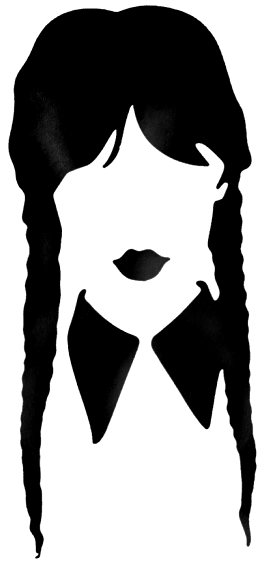
\includegraphics[height=1.35em]{figures/icons/mira-silhouette.png}}{}}}\enspace{\scshape\color{black}Scene}\enspace\textperiodcentered\enspace{\bfseries #1}\pdblockheadingend{\itshape #2}}%
    \end{tcolorbox}\par\addvspace{8pt plus 2pt}%
  }%
  \long\def\xrefbox#1{\par\pd@settle\addvspace{4pt}\noindent\pd@marginhead{See also}{\small #1}\par\addvspace{4pt}}%
  % A generic "Thesis" margin label does not identify which claim matters.
  % Keep the prose; use an authored keyidea head only when it adds meaning.
  \long\def\pdthesis#1{\par\pd@settle\addvspace{6pt plus 1pt}\noindent#1\par\addvspace{6pt plus 1pt}}%
  \long\def\pullquote#1{\pdthesis{#1}}%
}
\makeatother

% Shared visual language for the Book's figures -- version 2.
% Twin: book/figures/pd-figure-language.tex (byte-identical; edit both).
% The standard behind it, the migration from v1 and the QA loop live in
% skills/tikz-diagram-craft/ (SKILL.md, references/figure-standard.md).
%
% This file defines voices, hues, weights and marks -- not layouts.  Every
% figure still chooses a grammar from its reader question.
%
% ===========================================================================
% 1.  THE TYPE LADDER.  Three voices, one size, each tied to a role.
%       pd title   bold      panel titles, row and actor heads, column heads
%       pd label   upright   node text, state names, axis titles, tick words,
%                            relation words on an edge, badge numerals
%       pd note    italic    the one annotation a figure is allowed
%     `pd tag` is the label voice knocked out of the page, for a word that
%     must sit near a rule.  `pd kind` (small caps) is a one- or two-word kind
%     tag, never a title.  Every piece of figure text is mixed case; \texttt
%     only for identifiers that are literally code; math mode for symbols.
%
% 2.  THE COLOUR SYSTEM.  Hue is meaning, and the meanings cross chapters.
%     The figure's own subject is drawn in the CHAPTER hue (`pd focus ...`),
%     resolved from \pdcurrentchaptercolor, which the Book sets per chapter;
%     a fragment declares its standalone fallback with \pdfigurehue{...}.
%     Anything else the figure names takes its concept hue:
%       pd truth       pdcobalt   kernel, truth, the thing being specified
%       pd legible     pdteal     legibility, digest, inspection
%       pd ready       pdhealth   ready, coordinated, admitted, passing
%       pd protocol    pdindigo   protocol, federation, the wire
%       pd identity    pdviolet   identity, continuity, a card, an ID
%       pd reputation  pdrust     reputation, trust earned over time
%       pd value       pdgold     economy, value, settlement, payment
%       pd breach      pderror    breach, refusal, revocation, correction
%       pd warn        pdamber    warning; rules and stripes only, never text
%     Each concept X yields X, X rule, X arrow, X state, X fill, X datum and
%     X label.  Two to four hues a figure; colour is always doubled by shape,
%     dash, weight or a word (breach and warn are dashed as well as coloured).
%
% 3.  THE WEIGHT LADDER.  Exactly three weights, .5 / .9 / 1.6 pt
%     (1 : 1.8 : 3.2).  .5: hairline, guide, tick, artifact edge, fill edge,
%     mark outline, badge.  .9: rule, arrow, state edge, concept arrow.
%     1.6: spine, focus rule, focus and concept state edges, concept rule.
%     A reader sees which line is the subject.  Tips scale with the stroke.
%
% 4.  THE SURFACE LADDER.  pd state (page ground, ink edge) < pd artifact
%     (page ground, grey edge, subordinate) < pd focus state and the concept
%     states (24 % tint, edged in the same hue).  Text is always ink.  A
%     terminal state has a double boundary; an automaton's states are circles
%     (`pd automaton state/focus/terminal`); a ledger's pools are buckets
%     joined by pipes (`pd bucket`, `pd pipe`); a trust boundary is a dashed
%     rectangle (`pd trust boundary`).
%
% 5.  THE GROUND.  Body pages print on white, so every knockout and every
%     neutral surface is `pdpage` (white), never cream: a cream backing on a
%     white page reads as a sticker, which is what v1's figures were covered
%     in.  Neutral regions (Gantt bands, wells) are a warm grey tint.
%
% 6.  EDITIONS.  The Book sets \pdedition (maritime | swiss | technical) and
%     figures/pd-figure-language-<edition>.tex restyles the same names, so one
%     drawing renders in each edition's character.  A fragment that names a
%     raw colour (hhteal, pdcobalt!40, blue) bypasses this; name a role.
% ===========================================================================
% Libraries every v2 mark needs (diamonds, braces, markings), and
% pgfplots for computed plots. This file is \input in every preamble (the
% Book's and each standalone chapter's), so a plot works in all of them.
\usetikzlibrary{arrows.meta,matrix,patterns.meta,positioning,calc,fit,
  backgrounds,shapes.geometric,shapes.multipart,shapes.misc,decorations.pathreplacing,
  decorations.markings,quotes,intersections}
\RequirePackage{pgfplots}
\pgfplotsset{compat=1.18}
\usepgfplotslibrary{fillbetween,groupplots}

\colorlet{pdpage}{white}

% --- the chapter hue, resolved late --------------------------------------
% \pdfigurehue{pdindigo} on the line before a tikzpicture names the hue the
% figure is drawn in when it is compiled outside the Book (a standalone
% chapter, or the skill's renderer).  Inside the Book the preamble has already
% defined \pdcurrentchaptercolor and the chapter opener sets it, so there the
% opener wins and \providecommand does nothing.  Local to the figure's group.
\newcommand{\pdfigfraghue}{pdcobalt}
\newcommand{\pdfigurehue}[1]{%
  \renewcommand{\pdfigfraghue}{#1}%
  \providecommand{\pdcurrentchaptercolor}{#1}}
\newcommand{\pdsetfocushue}{%
  \ifdefined\pdcurrentchaptercolor
    \colorlet{pdfocus}{\pdcurrentchaptercolor}%
  \else
    \colorlet{pdfocus}{\pdfigfraghue}%
  \fi}
\colorlet{pdfocus}{pdcobalt}

% ===========================================================================
% THE TYPOGRAPHIC LAW
% ===========================================================================
% Companion to the line-weight law in figures/pd-palette.tex (1px texture,
% 1.5px linework, 2px enclosure). Same shape of rule: name the roles, fix the
% values, one place.
%
% ONE SIZE. Every named text role in a figure is \pdfiglabelsize
% (= \footnotesize). Roles separate by WEIGHT, SLOPE, FAMILY and INK -- never
% by size. A fragment never writes a size command of its own; if a distinction
% needs making, it takes the role that makes it.
%
% Where the size comes from. Measured, not chosen:
%   \tiny  \scriptsize  \footnotesize  \small  \normalsize
%   5.23    6.97          8.72           9.55    10.46  pt   Book (10.5pt
%                                                            Pagella, 4.5in
%                                                            column, 7x10in)
%   5.98    7.97          8.97           9.96    10.91  pt   standalone chapter
%                                                            (11pt Latin Modern)
% \scriptsize renders at 6.97pt in the Book -- under figcheck's 7pt T1 floor
% before a single width promotion, so it is illegal by measurement, not taste.
% \footnotesize holds 8.72pt and still clears the floor at the 0.85 \resizebox
% limit craft-rules sets (7.41pt). It is also what the corpus already voted
% for: 78 of the 91 local font= declarations this law replaces were already
% \footnotesize, \footnotesize\bfseries or \footnotesize\itshape.
%
% \pdfigbasesize (= \small) is the tikzpicture's ambient size only, so an
% unstyled node is never SMALLER than a styled one; every named role steps
% down exactly one notch from it and none steps down twice.
%
% ONE FACE, AND IT IS THE DOCUMENT'S. \pdfiglabelfamily is empty by default,
% which means figure type inherits whatever face the document is setting --
% Palatino in the Book, Computer Modern in a standalone chapter. Figures
% agreeing with EACH OTHER is not the goal; figures agreeing with the
% paragraph beside them is. A fragment therefore never names a family. Not
% \sffamily (which resolves to Latin Modern Sans against a Computer Modern
% page and reads as a foreign object on it), not \rmfamily, not
% \fontfamily{...}. P18 in tikz_precheck.py is an error for exactly that.
% An edition MAY substitute a face -- the Swiss and technical editions set
% \pdfiglabelfamily to \pdgrotesk, because grotesk display is their declared
% character -- and it does so in ONE command in ONE file, so the substitution
% is a decision on the record rather than an accident in a fragment. The
% only family a fragment may ask for is the identifier one, and it asks for
% it by role (pd mono label / \pdfiglabelmono), never by \ttfamily.
%
% What the roles are, and what each one is for:
%   pd panel title        bold        the name of a panel
%   pd row label          bold        an actor/row name east of its lane
%   pd reverse row label  bold, cream a row name sitting on a dark band
%   pd axis label         regular     an axis title or a tick numeral
%   pd direct label       regular     a value or name riding its own mark
%   pd reverse label      regular, cream  a direct label on a dark band
%   pd mono label         mono        an identifier, path, or literal
%   pd verdict            bold        a terminal outcome stamp (CLEAR, REJECT)
%   pd note               italic      one aside per figure
%   pd legend             regular     a pgfplots legend entry
%   pd state / terminal / actor / artifact / decision   node text
%   pd axis               the whole pgfplots typographic block, one key
%   \pdfigsub             a gloss line under a heading INSIDE a node
%   \pdfigmath            math carrying a sub/superscript, inside a label
%
% A fragment that needs a compound style of its own composes it from a role
% above (`gate/.style={pd decision,minimum width=2cm}`), or, where no role
% fits, from the \pdfiglabel* handles here. It never writes a raw size
% command: P16 in skills/harbor-chartwork/scripts/tikz_precheck.py is an
% error for exactly that, and P10/P11 have been errors for \tiny and
% \scriptsize since before this law.
%
% What does NOT transfer from the screen rules these roles otherwise follow.
% The dataviz method those rules come from assumes an interactive chart: a
% tooltip carries any value a label could not fit, a filter row rescopes the
% view, hover lifts the hovered mark. A printed page has none of that, and the
% absence is not a defect to design around. The INTENT of the tooltip rule --
% "every value is reachable without gating" -- does transfer, and on this page
% it is discharged somewhere else: the value is in the caption, in the margin
% apparatus, or in the chapter's own worked example. So a label that will not
% fit inside its mark moves outside the mark or is dropped to the caption; it
% is never shrunk to fit, because there is no size below \footnotesize to shrink
% to, and never clipped. Do not add a hover affordance, a legend toggle, or a
% filter to a figure in this book.
%
% IDENTIFIERS GET ONE SPELLING. A key, a cell id, a file name or any other
% literal a reader could type is set in `pd mono label` (or \pdfiglabelmono
% inside a compound style), spelled exactly as the code spells it: sk_A, not
% skA and not sk with a subscript A; card0, not card-nought and not a Unicode
% subscript zero. A figure that shows the same identifier two ways has told
% the reader they are two things. The subscripted form belongs to MATHEMATICS
% ($\kappa_7$, an index into a sequence) and the literal form to CODE -- one
% figure may use both, for different objects, but never both for the same
% one. (A precheck for two spellings of one identifier inside a fragment is
% being added on another branch; this is the convention it will enforce.)
%
% SHAPE IS A CHANNEL, AND IT HAS TO SURVIVE THE PRINT SIZE. pd datum, pd
% focus datum and pd caution datum carry three different forms, because the
% house palette is three low-chroma print inks and every distinction it makes
% has to be doubled by something that is not colour. That only counts if the
% form is still legible at 2.1-2.7 pt: an edition that flattens all three to
% one form has removed the second channel and left the figure separating its
% classes by hue alone, which fails in greyscale and for a colour-blind
% reader. Any edition override that restyles a datum must keep three
% distinguishable forms, and must be checked on a render at 1.0x, not
% reasoned about from the point sizes.
%
% One screen rule that does NOT bind here, and why. "Text never wears the data
% colour" exists because a light categorical hue is illegible as text on a
% light surface. The house figure hues are print inks, not screen hues --
% hhink #1B1712, hhteal #00564C, hhamber #6B4500 -- and all three clear text
% contrast on cream, so a label MAY wear its series' ink to bind itself to a
% curve, which is direct labelling and saves a legend. The rule that survives
% is the reason behind it: text wears one of those three inks at full
% strength, or hhink!80!hhgray for recessive furniture, and nothing else. A
% tint of an ink (text=hhgray, text=hhteal!60) is not a role; it is a fade.
% ===========================================================================

\providecommand{\pdfiglabelfamily}{}            % an edition may set \pdgrotesk
\providecommand{\pdfiglabelsize}{\footnotesize} % every named text role
\providecommand{\pdfigbasesize}{\small}         % the picture's ambient size
\providecommand{\pdfiglabel}{\pdfiglabelfamily\pdfiglabelsize}
\providecommand{\pdfiglabelbold}{\pdfiglabel\bfseries}
\providecommand{\pdfiglabelitalic}{\pdfiglabel\itshape}
\providecommand{\pdfiglabelmono}{\pdfiglabelsize\ttfamily}
% The one role that is not a node style, because it lives INSIDE a node's text:
% the second line under a heading that glosses it ("reviewer role / obligation +
% capability + authority"). Every fragment that needed it reached for \tiny or
% \scriptsize, which is how seven \tiny and twelve \scriptsize survived P10/P11
% as hard errors in the corpus. It steps down by SLOPE and WEIGHT, not size, so
% it stays legible and stays legal, and it touches neither family nor ink --
% which is what lets it sit on a reversed node without vanishing.
\providecommand{\pdfigsub}{\mdseries\itshape}
% The one place the law's own size is not the right size.
%
% Measured, both preambles, on a subscripted label inside `pd direct label`:
%
%              base glyph   subscript   subscript as % of base
%   chapter      8.97pt       5.98pt            66.7%
%   Book         8.72pt       6.36pt            72.9%
%   promoted    10.91/10.46   7.97/7.64
%
% An earlier version of this comment said those subscripts are "under figcheck's
% 7pt T1 floor". They are not, and the correction is worth more than the claim
% was. T1 has TWO bands: running text is held to 7.0pt, and a span of three
% glyphs or fewer -- a sub/superscript, a tick numeral -- is held to 5.9pt
% (T1_SHORT_SPAN_PT). That second band is not a loophole. A subscript is set at
% roughly 70% of its base by every typesetter that has ever existed; holding one
% to the running-text floor would mean either no subscripts in figures at all,
% or a figure whose base type is 10pt against 8.72pt body text.
%
% So \pdfigmath is NOT a T1 remedy, and using it as one is how a rule gets
% applied where it does not belong. It exists because 5.98pt clears the
% short-span band by 0.08pt, and 0.08pt is not a margin: a font substitution, an
% edition that nudges \pdfigbasesize, or a chapter that loads a different math
% font puts that subscript under the band with nobody having decided anything.
% Promotion puts it at 7.97/7.64pt -- over even the running-text floor -- while
% the base glyph stays close enough to its neighbours that the label still reads
% as one label.
%
% Use it ONLY for a math group that carries a sub- or superscript. Plain math
% takes the label's own size like any other text, and P22 in tikz_precheck.py is
% an error if it does not.
\providecommand{\pdfigmath}{\normalsize}

% ---------------------------------------------------------------------------
% THE GUIDE DASH, IN ABSOLUTE POINTS, IN ONE PLACE.
%
% `pd guide` used to read `line width=.45pt,densely dotted`. `densely dotted`
% expands to `dash pattern=on \pgflinewidth off 1pt`, and \pgflinewidth is read
% when the KEY is processed, not when the path is stroked. So the Swiss
% edition's `pd guide/.append style={draw=hhink!40,line width=.5pt}` widened the
% stroke and left the dash at the .45pt already baked into it. The canonical
% Book therefore shipped a 0.448pt dot on a 0.498pt stroke.
%
% MEASURED IN THE SHIPPED ARTIFACT, not in a probe: 50 guide strokes sampled
% pixel by pixel in the committed coordination-papers-mega-volume.pdf, at 150
% dpi / 1.0x.
%
%   on 0.448pt = 0.93 device px -- UNDER ONE PIXEL; off 0.996pt = 2.08 px
%   the dash DECLARES 69% of each line's length as gap
%   only 34% of each line's pixels actually reach paper
%   35.4% of three-period windows contain NO pixel that reaches paper at all
%
% That last number is the defect. The gap (2.08 px) is narrower than the
% antialias spread of a 0.93 px stroke, so as the pattern's phase drifts along a
% line the gaps fill in: over a third of every guide's length there is no gap
% left and it is a continuous grey stroke, while the rest of the same line still
% reads as dots. The ink arrives. The DOTTEDNESS does not. A reader sees one
% line that is dotted here and solid there, and no author chose that.
%
% Twenty-five of the corpus's thirty-six guide draws use dottedness to mean
% "this line is not a drawn edge", so twenty-five of them were making a
% distinction the page does not carry.
%
% After, same measurement, same probe geometry, Book preamble:
%   on 1.2pt = 2.50 px, off 2.0pt = 4.17 px, stroke .7pt = 1.45 px
%   0.0% of three-period windows are without paper -- every gap survives,
%     at every phase
%   50% of pixels reach paper against 62.5% declared, the shortfall now being
%     the stroke's antialias skirt rather than the whole signal
%
% ON THE INK, because the obvious reading of this change is wrong. The BASE pair
% was never the problem: hhgray!62 against the hairline's hhgray!78 is 0.411
% against 0.517 of nominal ink, well apart. The problem is that the Book renders
% the SWISS edition (\pdedition defaults to swiss; the committed Book PDF is
% full of hhink!40 guides), where the pair was hhink!40 against hhink!45 -- 4.6%
% of the grey scale. Deleting the Swiss override, which is the right fix for the
% geometry, makes the base ink govern the Book too -- and hhgray!62 is 0.411
% against the Book hairline's 0.410. The same grey, to a thousandth. So the base
% ink has to move, or the dash would go back to carrying the whole distinction
% by itself, which is how this started.
%
% hhink!70 measured against the hairline, mean ink on the page at 150 dpi:
%   chapter  guide 0.0502  hairline 0.0790   guide is 64% of the hairline
%   Book     guide 0.0545  hairline 0.0671   guide is 81% of the hairline
% Per DOT it is 0.638 against 0.410 -- unmistakably a different mark. In MEAN it
% is still lighter than the hairline -- so it still recedes. Two channels, both
% working, instead of one that does not.
%
% The replacement is stated absolutely and measures phase-STABLE: every dot
% renders at the same weight wherever it falls on the grid (peak column ink
% 0.808, invariant across twelve sub-pixel offsets). It is a macro rather than
% three numbers because an edition that restates one of them and not the others
% is how this defect happened. The geometry is a LEGIBILITY FLOOR, not an
% edition's character: an edition may move the guide's ink, and states the
% geometry through these two macros so it cannot half-restate it.
%
% Any dash in this corpus is stated in absolute points. The `dotted` family
% (`dotted`, `densely dotted`, `loosely dotted`) derives its on-length from the
% line width and is therefore banned -- P23 in tikz_precheck.py. `dashed` and
% its relatives are absolute (on 3pt off 3pt) and are fine.
\providecommand{\pdguidewidth}{.7pt}
% Three lengths, not one macro holding the whole key: pgfkeys splits a key list
% on `,` and `=` before expanding anything (so a macro carrying `dash
% pattern=...` is read as one key NAME), and TikZ's dash-pattern scanner reads
% the literal words `on`/`off` without expanding a macro that hides them. A
% dimension after each word does expand, which is the seam that works.
\providecommand{\pdguideon}{1.2pt}
\providecommand{\pdguideoff}{2.0pt}

\tikzset{
  % --- picture level: one size, one default tip, the chapter hue -----------
  % A figure label is a name, not prose: it never hyphenates.
  pd figure/.style={font=\pdfiglabelfamily\pdfigbasesize,text=pdink,line cap=round,line join=round,
    >={Stealth[length=2.6pt 3.2,width=2.0pt 2.4]},/utils/exec=\pdsetfocushue,
    every node/.append style={execute at begin node={%
      \hyphenpenalty=10000\exhyphenpenalty=10000\relax}}},
%
  % --- 1. the voices ---------------------------------------------------------
  pd title/.style={font=\pdfiglabelbold,text=pdink,align=center},
  pd label/.style={font=\pdfiglabel,text=pdink,align=center},
  pd note/.style={font=\pdfiglabelitalic,text=pdinkmuted,align=left},
  pd kind/.style={font=\pdfiglabel\scshape,text=pdinkmuted,align=center},
  pd tag/.style={pd label,fill=pdpage,inner sep=1.7pt},
%
  % --- 4. surfaces -----------------------------------------------------------
  pd state/.style={pd label,draw=pdink,line width=.9pt,fill=pdpage,
    rounded corners=1pt,inner xsep=6pt,inner ysep=4.5pt,minimum height=7.4mm},
  % a terminal state carries a double boundary, as every automaton text draws it
  pd terminal/.style={pd state,double=pdpage,double distance=1.1pt,line width=.5pt},
  pd artifact/.style={pd label,draw=pdinkmuted!60,line width=.5pt,fill=pdpage,
    rounded corners=1pt,inner xsep=5pt,inner ysep=3.5pt,minimum height=6.2mm},
  pd panel/.style={draw=pdinkmuted!55,line width=.5pt,
    dash pattern=on 2.4pt off 2pt,rounded corners=2.5pt,inner sep=7pt,align=center},
  pd hatch/.style={pattern={Lines[angle=45,distance=4pt,line width=.3pt]},
    pattern color=pdinkmuted!70},
  pd neutral fill/.style={fill=pdinkmuted!12,draw=pdinkmuted!55,line width=.5pt},
%
  % --- 3. strokes ------------------------------------------------------------
  pd hairline/.style={draw=pdinkmuted!45,line width=.5pt},
  % Absolute dash, from the typographic law's three macros above: a guide is a
  % definite dotted construction line, darker per dot than the hairline and
  % lighter in mean ink. A lattice is the quiet continuous grid a figure stands on.
  pd guide/.style={draw=pdink!70,line width=\pdguidewidth,dash pattern=on \pdguideon off \pdguideoff},
  pd lattice/.style={draw=pdinkmuted!40,line width=.4pt},
  pd tick/.style={draw=pdinkmuted!75,line width=.5pt},
  pd rule/.style={draw=pdink,line width=.9pt},
  pd spine/.style={draw=pdink,line width=1.6pt},
  pd thin arrow/.style={draw=pdinkmuted!75,line width=.5pt,->},
  pd arrow/.style={pd rule,->},
  pd spine arrow/.style={pd spine,->},
%
  % --- the chapter hue, as the figure's focus --------------------------------
  pd focus rule/.style={draw=pdfocus,line width=1.6pt},
  pd focus arrow/.style={pd focus rule,->},
  pd focus state/.style={pd state,draw=pdfocus,line width=1.6pt,fill=pdfocus!24},
  % The single solid chapter-colour surface in a figure: use only for the
  % culmination or object the reader should name after five seconds. Editions
  % may render ordinary focus with a pale field while keeping this one solid.
  pd climax state/.style={pd focus state},
  % a member of the subject's set when the set, not one node, is the subject:
  % edged in the chapter hue, never filled, so the one solid node stays unique
  pd focus outline/.style={pd state,draw=pdfocus,line width=1.2pt,fill=pdpage},
  pd focus fill/.style={fill=pdfocus!24,draw=pdfocus,line width=.5pt},
  pd focus datum/.style={circle,fill=pdfocus,draw=pdpage,line width=.5pt,inner sep=2.6pt},
  pd focus label/.style={pd label,text=pdfocus!85!pdink},
%
  % --- marks -----------------------------------------------------------------
  pd datum/.style={circle,fill=pdink,draw=pdpage,line width=.5pt,inner sep=2.3pt},
  pd badge/.style={pd label,circle,draw=pdink,line width=.5pt,fill=pdpage,
    inner sep=.5pt,minimum size=5.0mm},
  pd focus badge/.style={pd badge,draw=pdfocus,line width=.9pt,fill=pdfocus!24},
  % --- conventions shared by every chapter (Critical Analysis, 2026-09-08) ---
  % Automata: states are circles, terminal (accepting) states double circles;
  % edge words are short action names; guards go in an aligned legend table.
  pd automaton state/.style={pd label,circle,draw=pdink,line width=.9pt,fill=pdpage,
    minimum size=11mm,inner sep=1pt},
  pd automaton focus/.style={pd automaton state,draw=pdfocus,line width=1.6pt,fill=pdfocus!24},
  pd automaton terminal/.style={pd automaton state,double=pdpage,double distance=1.1pt,
    line width=.5pt},
  pd initial/.style={draw=pdink,line width=.9pt,->},
  % Ledgers: asset pools are rectangular buckets (open at the top) joined by
  % directed pipes; the conserved sum is set as an equation under the rails.
  pd bucket/.style={pd label,draw=none,minimum width=2.2cm,minimum height=1.3cm,
    append after command={\pgfextra{\draw[draw=pdink,line width=.9pt]
      (\tikzlastnode.north west) -- (\tikzlastnode.south west)
      -- (\tikzlastnode.south east) -- (\tikzlastnode.north east);}}},
  pd pipe/.style={draw=pdink,line width=.9pt,double=pdpage,double distance=2.2pt,
    -{Stealth[length=3.4pt 2,width=5.2pt]}},
  pd focus pipe/.style={pd pipe,draw=pdfocus},
  % Trust boundaries: a dashed rectangle is the Dolev-Yao interface; a vector
  % that escapes it is drawn in pd breach and named.
  pd trust boundary/.style={draw=pdink,line width=.9pt,dash pattern=on 4pt off 2.4pt,
    rounded corners=0pt,inner sep=8pt},
  % a stroke that ends at a badge is shortened, so no rule touches the numeral
  pd to badge/.style={shorten >=2pt},
  pd from badge/.style={shorten <=2pt},
}

% ===========================================================================
% 7.  PLOTS.  A plot is computed by a committed script, never sketched.  `pd
%     axis` is the one axis grammar: two spines (left, bottom), ticks out, no
%     box, no grid unless asked (`pd grid`), tick words in the label voice,
%     numbers with a thin-space thousands separator, room outside the plot for
%     direct labels (clip=false).  Series are named at their ends, not in a
%     legend: `pd series` (ink), `pd focus series` (chapter hue), and
%     `pd X series` for a concept; breach and warn series are dashed.  A
%     region between curves is `pd focus fill`/`X fill` with fillbetween.
%     Width: `width=` is the plot box (scale only axis); leave about 1.6 cm
%     of the 11.4 cm column for the y tick words and title.
% ===========================================================================
\pgfplotsset{
  pd axis/.style={
    scale only axis,width=8.8cm,height=4.6cm,
    axis lines*=left,axis line style={draw=pdink,line width=.5pt,-},
    tick align=outside,major tick length=3pt,minor tick length=0pt,
    tick style={draw=pdink,line width=.5pt},
    tick label style={pd label,text=pdinkmuted},
    label style={pd label},title style={pd title},
    every axis title/.append style={yshift=-2pt},
    enlargelimits=false,clip=false,
    grid=none,
    legend style={draw=none,fill=none,font=\pdfiglabel},
    /pgf/number format/1000 sep={\,},
    every axis plot/.append style={line width=.9pt,line join=round,mark size=1.7pt},
  },
  pd grid/.style={ymajorgrids,major grid style={draw=pdinkmuted!30,line width=.4pt}},
  pd series/.style={draw=pdink,mark=*,mark options={fill=pdink,draw=pdpage,line width=.5pt,solid}},
  pd focus series/.style={draw=pdfocus,line width=1.6pt,mark=*,
    mark options={fill=pdfocus,draw=pdpage,line width=.5pt,solid}},
  pd muted series/.style={draw=pdinkmuted!70,line width=.9pt,mark=none},
}
\newcommand{\pdplotconcept}[2]{%
  \pgfplotsset{#1 series/.style={draw=#2,mark=*,
    mark options={fill=#2,draw=pdpage,line width=.5pt,solid}}}}
\pdplotconcept{pd truth}{pdcobalt}
\pdplotconcept{pd legible}{pdteal}
\pdplotconcept{pd ready}{pdhealth}
\pdplotconcept{pd protocol}{pdindigo}
\pdplotconcept{pd identity}{pdviolet}
\pdplotconcept{pd reputation}{pdrust}
\pdplotconcept{pd value}{pdgold}
\pgfplotsset{
  pd breach series/.style={draw=pderror,dash pattern=on 3.2pt off 2.2pt,mark=diamond*,
    mark options={fill=pderror,draw=pdpage,line width=.5pt,solid}},
  pd warn series/.style={draw=pdamber,dash pattern=on 3.2pt off 2.2pt,mark=none},
}

% ===========================================================================
% Supplied visual-guide primitives: native Book type, deliberate strokes,
% readable Stealth heads, open markers, and a quiet quantitative grid.
% These are opt-in: old diagrams need spacing review before thicker arrows.
\tikzset{
  pd guide step/.style={pd artifact,draw=pdink,fill=pdpage,line width=1pt,
    align=center,minimum height=40pt,inner xsep=5pt,inner ysep=6pt},
  pd guide arrow/.style={draw=pdcobalt,line width=1.15pt,
    -{Stealth[length=7pt,width=4.4pt]},shorten <=2pt,shorten >=2pt},
}
\newcommand{\pdflowstep}[4]{%
  \node[pd guide step,text width=#4] (#1) at #2 {#3};}
\newcommand{\pdflowlink}[2]{%
  \draw[pd guide arrow] (#1.east)--(#2.west);}
\pgfplotsset{
  pd evidence axis/.style={pd axis,
    axis line style={draw=pdink,line width=1pt,-},
    tick style={draw=pdink,line width=.8pt},
    grid=major,major grid style={draw=pdinkmuted!20,line width=.35pt},
    axis background/.style={fill=pdpage}},
  pd evidence measured/.style={draw=pdcobalt,line width=1.35pt,mark=*,
    mark size=2.6pt,mark options={fill=pdpage,draw=pdcobalt,line width=1.1pt}},
  pd evidence comparison/.style={draw=pdink,line width=1.1pt,
    dash pattern=on 4pt off 2.5pt,mark=square*,mark size=2.2pt,
    mark options={fill=pdink,draw=pdink,solid}},
}
% Analytic curves, not sampled observations. Integer samples preserve the
% meaning of reviewer count; callers set axes and name their assumptions.
\newcommand{\pdindependentmisses}[2]{%
  \addplot[pd evidence measured,domain=1:#2,samples=#2] {100*(1-#1)^x};}
\newcommand{\pdreviewcost}[1]{%
  \addplot[pd evidence measured,domain=1:#1,samples=#1] {x};}
% 8.  UML.  The Book's engineering diagrams use UML 2.5 notation, so a reader
%     who knows UML reads them without a key.  Four kinds:
%     STATE MACHINE  `pd uml state` (rounded), `pd uml focus state`, a
%       composite drawn with `pd uml composite` around its substates plus a
%       compartment of internal transitions; `pd uml initial` (filled dot),
%       `pd uml final` (bullseye), `pd uml choice` (diamond); transitions are
%       `pd uml transition` (open arrowhead) labelled  event [guard] / effect.
%     SEQUENCE  `pd uml head` (lifeline head), `pd uml lifeline` (dashed),
%       `pd uml activation` (thin bar), messages `pd uml sync` (filled head),
%       `pd uml async` (open head), `pd uml reply` (dashed, open head),
%       `pd uml fragment` + `pd uml fragment tag` for alt / opt / loop.
%     COMPONENT  `pd uml component` with \pdumlicon{node} (the component
%       glyph) and a <<component>> keyword; `pd uml port`; provided interface
%       \pdumlprovided{from}{to}{name} (lollipop), required \pdumlrequired (socket).
%     ERD (crow's foot)  `pd er entity` (rectangle split: name, then rows;
%       mark keys PK / FK in the row text), relationship lines `pd er rel`
%       with tips `er one`, `er many`, `er zero or one`, `er one or many`,
%       `er zero or many` at either end.
% ===========================================================================
\pgfdeclarearrow{
  name = pd crow,
  parameters = {\the\pgfarrowlength,\the\pgfarrowwidth},
  setup code = {%
    \pgfarrowssettipend{0pt}%
    \pgfarrowssetlineend{0pt}%
    \pgfarrowssetbackend{-\pgfarrowlength}%
    \pgfarrowsupperhullpoint{0pt}{.5\pgfarrowwidth}%
    \pgfarrowsupperhullpoint{-\pgfarrowlength}{0pt}%
    \pgfarrowssavethe\pgfarrowlength
    \pgfarrowssavethe\pgfarrowwidth},
  drawing code = {%
    \pgfsetdash{}{0pt}%
    \pgfpathmoveto{\pgfqpoint{-\pgfarrowlength}{0pt}}%
    \pgfpathlineto{\pgfqpoint{0pt}{.5\pgfarrowwidth}}%
    \pgfpathmoveto{\pgfqpoint{-\pgfarrowlength}{0pt}}%
    \pgfpathlineto{\pgfqpoint{0pt}{-.5\pgfarrowwidth}}%
    \pgfusepathqstroke},
  defaults = {length=2.4mm, width=3.0mm}
}
\tikzset{
  % state machine
  pd uml state/.style={pd state,rounded corners=4.5pt},
  pd uml focus state/.style={pd focus state,rounded corners=4.5pt},
  pd uml terminal/.style={pd terminal,rounded corners=4.5pt},
  pd uml composite/.style={draw=pdink,line width=.9pt,rounded corners=7pt,fill=none,inner sep=0pt},
  pd uml initial/.style={circle,fill=pdink,draw=none,minimum size=2.4mm,inner sep=0pt},
  pd uml final/.style={circle,draw=pdink,line width=.9pt,fill=pdpage,minimum size=3.6mm,inner sep=0pt,
    path picture={\fill[pdink] (path picture bounding box.center) circle (1.1mm);}},
  pd uml choice/.style={diamond,draw=pdink,line width=.9pt,fill=pdpage,minimum size=4.2mm,inner sep=0pt},
  pd uml transition/.style={pd rule,-{Straight Barb[length=2.2pt 2.2,width=4.4pt 2.2]}},
  pd uml focus transition/.style={pd focus rule,-{Straight Barb[length=2.2pt 2.2,width=4.4pt 2.2]}},
  pd uml breach transition/.style={pd rule,draw=pderror,dash pattern=on 3.2pt off 2.2pt,
    -{Straight Barb[length=2.2pt 2.2,width=4.4pt 2.2]}},
  % sequence
  pd uml head/.style={pd state,rounded corners=0pt,minimum height=6.8mm},
  pd uml lifeline/.style={draw=pdinkmuted!75,line width=.5pt,dash pattern=on 3pt off 2pt},
  pd uml activation/.style={draw=pdink,line width=.5pt,fill=pdpage,minimum width=2.2mm,inner sep=0pt},
  pd uml sync/.style={pd rule,-{Triangle[length=3.2pt 1.6,width=3.2pt 1.6]}},
  pd uml async/.style={pd rule,-{Straight Barb[length=2.4pt 2,width=4.4pt 2]}},
  pd uml reply/.style={pd rule,dash pattern=on 3pt off 2pt,-{Straight Barb[length=2.4pt 2,width=4.4pt 2]}},
  pd uml fragment/.style={draw=pdink,line width=.5pt,fill=none,inner sep=6pt},
  pd uml fragment tag/.style={pd label,font=\footnotesize\bfseries,draw=pdink,line width=.5pt,fill=pdpage,
    inner xsep=3pt,inner ysep=2pt,chamfered rectangle,chamfered rectangle corners=south east,
    chamfered rectangle xsep=2pt},
  % component
  pd uml component/.style={pd state,rounded corners=0pt,align=center,inner xsep=8pt,inner ysep=6pt,minimum height=11mm},
  pd uml port/.style={rectangle,draw=pdink,line width=.5pt,fill=pdpage,minimum size=2mm,inner sep=0pt},
  % ERD
  pd er entity/.style={pd label,rectangle split,rectangle split parts=2,rectangle split part align={center,left},
    draw=pdink,line width=.9pt,fill=pdpage,inner xsep=5pt,inner ysep=3pt,align=left,
    rectangle split part fill={pdinkmuted!12,pdpage}},
  pd er rel/.style={pd rule},
  er one/.tip={Bar[width=3.0mm,sep=1.2pt]Bar[width=3.0mm]},
  er many/.tip={Bar[width=3.0mm,sep=1.4pt]pd crow},
  er zero or one/.tip={Circle[open,length=1.8mm,width=1.8mm,sep=1.2pt,fill=pdpage]Bar[width=3.0mm]},
  er one or many/.tip={Bar[width=3.0mm,sep=1.4pt]pd crow},
  er zero or many/.tip={Circle[open,length=1.8mm,width=1.8mm,sep=1.2pt,fill=pdpage]pd crow},
}
% the component glyph, drawn in the top-right corner of a component node
\newcommand{\pdumlicon}[1]{%
  \begin{scope}[shift={($(#1.north east)+(-4.2mm,-2.6mm)$)},x=1mm,y=1mm]
    \draw[pdink,line width=.5pt,fill=pdpage] (0,-1.1) rectangle (2.6,1.1);
    \draw[pdink,line width=.5pt,fill=pdpage] (-.6,.25) rectangle (.6,.65);
    \draw[pdink,line width=.5pt,fill=pdpage] (-.6,-.65) rectangle (.6,-.25);
  \end{scope}}
% a provided interface (lollipop) from a node side to a point, with its name
\newcommand{\pdumlprovided}[3]{%
  \draw[pd rule] (#1) -- (#2);
  \draw[pd rule,fill=pdpage] (#2) circle (1.3mm);
  \node[pd label,anchor=south] at ($(#2)+(0,1.6mm)$) {#3};}
% a required interface (socket): a half-circle open toward the provider
\newcommand{\pdumlrequired}[4]{% from, to, name, facing angle of the socket's opening
  \draw[pd rule] (#1) -- (#2);
  \draw[pd rule] ($(#2)+(#4+90:1.9mm)$) arc[start angle=#4+90,end angle=#4+270,radius=1.9mm];
  \node[pd label,anchor=north] at ($(#2)+(0,-2.4mm)$) {#3};}

% --- 2. the concept map, as styles, so a drawing never chooses a hue --------
% An edition file may \renewcommand\pdconcept before the map below expands.
\newcommand{\pdconcept}[2]{%
  \tikzset{%
    #1/.style={draw=#2,text=pdink},
    #1 rule/.style={draw=#2,line width=1.6pt},
    #1 arrow/.style={draw=#2,line width=.9pt,->},
    #1 state/.style={pd state,draw=#2,line width=1.6pt,fill=#2!24},
    #1 fill/.style={fill=#2!24,draw=#2,line width=.5pt},
    #1 datum/.style={circle,fill=#2,draw=pdpage,line width=.5pt,inner sep=2.6pt},
    #1 label/.style={pd label,text=#2!85!pdink},
  }}

% --- 6. the edition layer, loaded before the concept map expands ----------
\ifdefined\pdedition\IfFileExists{figures/pd-figure-language-\pdedition.tex}{\input{figures/pd-figure-language-\pdedition}}{}\fi

\pdconcept{pd truth}{pdcobalt}
\pdconcept{pd legible}{pdteal}
\pdconcept{pd ready}{pdhealth}
\pdconcept{pd protocol}{pdindigo}
\pdconcept{pd identity}{pdviolet}
\pdconcept{pd reputation}{pdrust}
\pdconcept{pd value}{pdgold}
\pdconcept{pd breach}{pderror}
\pdconcept{pd warn}{pdamber}
% Breach and warning read as refusals, so they are dashed as well as
% coloured, and a breach mark is a diamond where every other mark is a circle.
% Amber is never text (3.71:1 on white); a warn label is set in ink.
\tikzset{
  pd breach rule/.append style={dash pattern=on 3.2pt off 2.2pt},
  pd breach arrow/.append style={dash pattern=on 3.2pt off 2.2pt},
  pd warn rule/.append style={dash pattern=on 3.2pt off 2.2pt},
  pd warn arrow/.append style={dash pattern=on 3.2pt off 2.2pt},
  pd breach datum/.append style={diamond},
  pd warn label/.style={pd label},
}

% ===========================================================================
% v1 NAMES.  Kept so every existing fragment still compiles; they resolve to
% the v2 roles, so an untouched figure inherits the ladder.  New work uses the
% v2 names (skills/tikz-diagram-craft/references/migration-v1-to-v2.md).
% ===========================================================================
\tikzset{
  pd row label/.style={pd title,anchor=east},
  pd panel title/.style={pd title,align=left},
  pd axis label/.style={pd label},
  % Direct labels sit beside their mark; they do not erase a line or box
  % underneath themselves. A label that needs a paper knockout is misplaced
  % and must be moved, not given an invisible patch.
  pd direct label/.style={pd tag,fill=none,align=left},
  pd actor/.style={pd state},
  pd boundary/.style={pd panel},
  pd caution rule/.style={pd breach rule},
  pd caution arrow/.style={pd breach arrow},
  pd caution fill/.style={pd breach fill},
  pd caution datum/.style={pd breach datum},
}

% ===========================================================================
% Roles named on main by the typographic law (#10191), expressed on the v2
% roles so an edition's .append style on the parent reaches them. `pd danger`
% is main's name for what v2 calls `pd breach` (red, dashed, diamond marks);
% both names resolve to one family. Main's hairline-boxed fact badge is
% `pd fact badge`: v2's `pd badge` is the numbered guard/step marker.
% ===========================================================================
\tikzset{
  pd danger rule/.style={pd breach rule},
  pd danger arrow/.style={pd breach arrow},
  pd danger fill/.style={pd breach fill,text=pdink},
  pd danger datum/.style={pd breach datum},
  pd ink fill/.style={fill=pdink,draw=pdink,line width=.4pt,text=pdpage},
  pd decision/.style={pd state,diamond,aspect=1.55,font=\pdfiglabelbold,
    minimum height=0pt,inner xsep=3pt,inner ysep=3pt},
  pd mono label/.style={pd direct label,font=\pdfiglabelmono,inner xsep=2.5pt,inner ysep=2.5pt},
  pd verdict/.style={pd direct label,font=\pdfiglabelbold},
  pd reverse label/.style={pd direct label,text=pdpage,fill=none},
  pd reverse row label/.style={pd row label,text=pdpage},
  pd legend/.style={font=\pdfiglabel,text=pdink,draw=none,fill=none},
  pd kind tag/.style={pd kind,align=right},
  pd fact badge/.style={pd hairline,font=\pdfiglabel,text=pdink,align=center,
    inner sep=2.4pt,fill=none},
}

% Small reusable marks.  They deliberately avoid prose-bearing boxes.
\newcommand{\pdfigaxis}[4]{%
  \draw[pd rule,->] (#1,#2) -- (#3,#2);
  \node[pd label,anchor=west] at (#3,#2) {#4};
}
\newcommand{\pdfigvaxis}[4]{%
  \draw[pd rule,->] (#1,#2) -- (#1,#3);
  \node[pd label,anchor=south] at (#1,#3) {#4};
}

% Native-size, object-based evidence figures; shared by Book and chapters.
% Shared approved Swiss evidence drawing primitives. Keep both chapter roots identical.
\ifdefined\pdSwissEvidenceLoaded\else
\def\pdSwissEvidenceLoaded{1}
% Real ink-box gate; no declared coordinate envelope can substitute for this.
\newsavebox{\sgEvidenceBox}
\newcommand{\SGMeasuredFigure}[2]{%
  \sbox{\sgEvidenceBox}{#2}%
  \typeout{SG-GEOMETRY: #1,width=\the\wd\sgEvidenceBox,height=\the\dimexpr\ht\sgEvidenceBox+\dp\sgEvidenceBox\relax}%
  \ifdim\wd\sgEvidenceBox>325.215pt
    \PackageError{swiss-evidence}{Figure #1 exceeds the Book column}{Recompose at native text size; do not scale.}%
  \fi
  \usebox{\sgEvidenceBox}}
% Parent redraws after rejection of lab specimens 01,04,06.
% All coordinates are physical TeX points; no resizebox or transformed fonts.
\usetikzlibrary{arrows.meta,calc}
% Aliased onto the house palette (figures/pd-palette.tex), not \definecolor'd
% as independent HTML values: an edition that restyles pdcobalt/pdteal/...
% now restyles every SG figure with it. The six values were already
% bit-identical matches for pdcobalt/pdteal/pdviolet/pdamber/pderror/pdink;
% the alias turns that into a guarantee instead of a coincidence.
\colorlet{sgBlue}{pdcobalt}
\colorlet{sgTeal}{pdteal}
\colorlet{sgViolet}{pdviolet}
\colorlet{sgAmber}{pdamber}
\colorlet{sgRed}{pderror}
\colorlet{sgInk}{pdink}
\definecolor{sgGrid}{HTML}{D8C7A6}
% The one house size, inheriting the document's own face (the typographic
% law in pd-figure-language.tex): no \sffamily leak, no local \fontsize.
\newcommand{\SGType}{\pdfiglabel}
\tikzset{sg/base/.style={x=1pt,y=1pt,line cap=butt,line join=miter,
  every node/.style={font=\SGType,inner sep=0pt,text=sgInk}},
  sg/arrow/.style={-{Stealth[length=4.5pt,width=3.6pt]},draw=sgInk,line width=.85pt},
  sg/grid/.style={draw=sgGrid,line width=.3pt},
  sg/hash/.style={draw=sgBlue,fill=sgBlue!7,line width=1pt,minimum width=53pt,
    minimum height=27pt,inner sep=4pt,align=center},
  sg/sibling/.style={draw=sgAmber,fill=sgAmber!10,line width=1pt,minimum width=51pt,
    minimum height=27pt,inner sep=4pt,align=center},
  sg/check/.style={draw=sgInk,fill=white,line width=1pt,minimum width=92pt,
    minimum height=30pt,inner sep=5pt,align=center}}

% A folded record, not an undifferentiated rounded node. Width/height are pt.
\newcommand{\SGDocument}[6]{%
  \begin{scope}[shift={#2}]
    \path[draw=sgInk,fill=#5,line width=.85pt]
      (0,0)--({#3-7},0)--(#3,7)--(#3,#4)--(0,#4)--cycle;
    \draw[sgInk,line width=.65pt] ({#3-7},0)--({#3-7},7)--(#3,7);
    \node[minimum width=#3pt,minimum height=#4pt,text width=\dimexpr#3pt-12pt\relax,
      align=center] (#1) at ({#3/2},{#4/2}) {#6};
  \end{scope}}

\newcommand{\SGSurvival}{%
\begin{tikzpicture}[sg/base]
  % Three complete probability decades, percentages rather than tiny exponents.
  \foreach \x in {0,1,...,6}{\draw[sg/grid] ({35+30*\x},20)--({35+30*\x},140);}
  \foreach \y/\lab in {20/{0.1\%},60/{1\%},100/{10\%},140/{100\%}}{%
    \draw[sg/grid] (35,\y)--(215,\y);
    \draw[sgInk,line width=.65pt] (32,\y)--(35,\y);
    \node[anchor=east] at (28,\y) {\lab};}
  \draw[sgInk,line width=.85pt] (35,140)--(35,20)--(215,20);
  \foreach \x in {0,2,4,6}{%
    \draw[sgInk,line width=.65pt] ({35+30*\x},20)--({35+30*\x},17);
    \node[anchor=north] at ({35+30*\x},12) {$\x$};}
  \node[rotate=90] at (-9,80) {jobs still running (log scale)};
  \node[anchor=north] at (125,-5) {duration / mean duration};
  \draw[sgBlue,line width=1.5pt,domain=0:6,samples=100]
    plot ({35+30*\x},{140-120*ln(1+\x/2)/ln(10)});
  \draw[sgViolet,line width=1.2pt,dash pattern=on 4pt off 2.5pt,domain=0:6,samples=100]
    plot ({35+30*\x},{140-40*\x/ln(10)});
  % Endpoint leaders have allocated space; text does not lie on a curve.
  \draw[sgBlue,line width=.8pt] (215,67.75)--(224,67.75);
  \node[anchor=west,text=sgBlue,font=\SGType\bfseries] at (230,73) {Lomax};
  \node[anchor=west,text=sgBlue] at (230,60) {1.56\%};
  \draw[sgViolet,line width=.8pt,dashed] (215,35.77)--(224,35.77);
  \node[anchor=west,text=sgViolet,font=\SGType\bfseries] at (230,40) {exponential};
  \node[anchor=west,text=sgViolet] at (230,27) {0.248\%};
\end{tikzpicture}}

\newcommand{\SGTiming}{%
\begin{tikzpicture}[sg/base,y=-1pt]
  % This bracket spans COMMIT TO SYNC. It is not a range of hypothetical syncs.
  \path[draw=sgAmber!35,fill=sgAmber!9,line width=.5pt] (39,19) rectangle (253,49);
  \draw[sgAmber,line width=1pt] (39,18)--(39,9)--(253,9)--(253,18);
  \node[anchor=south,text=sgAmber,font=\SGType\bfseries] at (146,5) {?};
  \draw[sgInk,line width=.9pt] (39,27)--(39,45) (253,27)--(253,45);
  \draw[{Stealth[length=4.5pt,width=3.6pt]}-{Stealth[length=4.5pt,width=3.6pt]},
    sgAmber,line width=1.3pt] (40,36)--(252,36);
  \node[anchor=north,font=\SGType\bfseries] at (39,52) {commit};
  \node[anchor=north,font=\SGType\bfseries] at (253,52) {WAL sync};
  \node[anchor=west] at (0,86) {heartbeats received};
  \foreach \x/\label in {57/{s_1},117/{s_2},194/{s_3},278/{s_4}}{%
    \draw[sgViolet!70,dashed,line width=.55pt] (\x,104)--(\x,145);
    \node[anchor=south,text=sgViolet] at (\x,101) {$\label$};}
  \path[draw=sgAmber!35,fill=sgAmber!9,line width=.5pt] (158,108) rectangle (243,142);
  \draw[sg/grid] (0,139)--(306,139);
  \draw[sgTeal,line width=1.4pt]
    (0,132)--(25,132)--(25,116)--(33,116)--(33,132)
    --(85,132)--(85,116)--(93,116)--(93,132)
    --(145,132)--(145,116)--(153,116)--(153,132)--(306,132);
  \draw[sgRed,line width=1pt] (243,106)--(243,145);
  \node[anchor=north,text=sgRed] at (243,149) {deadline};
  \draw[sg/arrow] (0,174)--(306,174);
  \node[anchor=north east] at (306,179) {time};
\end{tikzpicture}}

\newcommand{\SGInclusion}{%
\begin{tikzpicture}[sg/base,y=-1pt]
  % Two independent inputs: a supplied proof and an issuer-authenticated root.
  \node[anchor=north west,font=\SGType\bfseries,text width=158pt,align=left] at (0,0)
    {Recompute from the receipt};
  \node[anchor=north west,font=\SGType\bfseries,text width=118pt,align=left] at (193,0)
    {Authenticate\\the checkpoint};
  \draw[sg/grid,step=15pt] (0,29) grid (175,194);
  \SGDocument{receipt}{(4,35)}{49}{34}{sgViolet!9}{receipt $P$}
  \node[sg/hash] (leaf) at (29,103) {$a=H_L(P)$};
  \node[sg/sibling] (sibone) at (108,103) {sibling $b$};
  \node[sg/hash] (inner) at (68,146) {$u=H_N(a,b)$};
  \node[sg/sibling] (sibtwo) at (146,146) {subtree $c$};
  \node[sg/hash,fill=sgBlue,text=white,minimum width=100pt] (computed) at (107,190)
    {$R'=H_N(u,c)$};
  \draw[sg/arrow,draw=sgViolet] (receipt.south)--(leaf.north);
  \draw[sg/arrow,draw=sgBlue] (leaf.south)--(inner.north west);
  \draw[sg/arrow,draw=sgAmber] (sibone.south)--(inner.north east);
  \draw[sg/arrow,draw=sgBlue] (inner.south)--(computed.north west);
  \draw[sg/arrow,draw=sgAmber] (sibtwo.south)--(computed.north east);
  \SGDocument{checkpoint}{(211,37)}{85}{48}{sgTeal!8}{signed root $R^*$\\size $n=4$\\signature $\sigma$}
  % The trusted key is an external input, not something the prover supplies.
  \draw[sgInk,line width=1pt] (218,113) circle (3.5pt);
  \draw[sgInk,line width=1pt] (221.5,113)--(233,113) (230,113)--(230,117) (233,113)--(233,117);
  \node[anchor=west] at (239,113) {trusted $pk_I$};
  \node[sg/check,minimum width=84pt] (verify) at (260,158) {verify $\sigma$\\result $A$};
  \draw[sg/arrow,draw=sgTeal] (checkpoint.east)--(311,61)--(311,158)--(verify.east);
  \draw[sg/arrow] (247,123)--(247,138)--(verify.north);
  \node[sg/check,minimum width=112pt,minimum height=34pt] (compare) at (164,245)
    {$A\ \land\ (R'=R^*)$};
  \draw[sg/arrow,draw=sgBlue] (computed.south)--(107,220)--(compare.north west);
  \draw[sg/arrow,draw=sgTeal] (verify.south)--(260,214)--(compare.north east);
  \node[anchor=east,text=sgTeal] at (250,204) {$R^*,A$};
  \node[draw=sgTeal,fill=sgTeal,text=white,minimum width=90pt,
    minimum height=27pt,font=\SGType\bfseries] (accept) at (76,299) {accept inclusion};
  \node[draw=sgRed,fill=white,text=sgRed,line width=1.2pt,minimum width=90pt,
    minimum height=27pt,font=\SGType\bfseries] (reject) at (256,299) {reject proof};
  \draw[sg/arrow,draw=sgTeal] (compare.south west)--(108,279)--(76,279)--(accept.north);
  \draw[sg/arrow,draw=sgRed] (compare.south east)--(220,279)--(256,279)--(reject.north);
  \node[anchor=south,text=sgTeal] at (82,275) {true};
  \node[anchor=south,text=sgRed] at (248,275) {false};
\end{tikzpicture}}

% Reusable geometry; load after swiss-redraws.tex. Real points, no scaling.
\newcommand{\SGDatabase}[4]{%
  \begin{scope}[shift={#2}]
    \path[draw=#3,fill=#3!7,line width=.9pt]
      (0,4)--(0,32) arc[start angle=180,end angle=360,x radius=24pt,y radius=5pt]
      --(48,4) arc[start angle=0,end angle=-180,x radius=24pt,y radius=5pt];
    \draw[draw=#3,fill=#3!7,line width=.9pt] (24,4) ellipse[x radius=24pt,y radius=5pt];
    \node[minimum width=48pt,minimum height=37pt,align=center] (#1) at (24,18) {#4};
  \end{scope}}

% Reader question: How do overlapping requests become ordered records?
% Evidence: schematic two-client history, not a runtime observation.
% Each request precedes commit 1; each reply follows its own committed record.
\newcommand{\SGWriterSequence}{%
\begin{tikzpicture}[sg/base,y=-1pt]
  % Recomposed at native size: a 22-character mono request label no longer
  % fits a 118pt lane gap at \pdfiglabelmono, so the HTTP verb is shortened
  % to the identifier it names and the resource it names ("auth.ts") moves
  % to the lane header, where it reads once instead of twice.
  \foreach \x/\lanelabel in {35/{{\pdfigmath$\alpha_{\text{auth}}$} (claude)},153/{Kernel (single writer)},275/{{\pdfigmath$\alpha_{\text{bill}}$} (codex)}}{
    \node[anchor=south,font=\pdfiglabelbold,align=center] at (\x,0) {\lanelabel};
    \draw[sg/grid] (\x,9)--(\x,237);}
  % Both invocations precede the first commit: overlapping client requests.
  \draw[sg/arrow,draw=sgViolet] (35,29)--(153,29);
  \node[anchor=south,text=sgViolet,font=\pdfiglabelmono] at (94,24) {POST /claims};
  \draw[sg/arrow,draw=sgAmber] (275,57)--(153,57);
  \node[anchor=south,text=sgAmber,font=\pdfiglabelmono] at (214,52) {POST /claims};
  % commit 1 succeeds: drawn in the kernel's own hue. commit 2 is the
  % kernel's WAL record of a REFUSAL, not a second grant -- it is drawn in
  % the breach hue so the outcome is doubled by colour, not stated in prose
  % alone (the typographic law's "colour is always doubled" rule). The
  % "lock held" highlight band is gone: at native size it ran directly
  % behind this text, which figcheck reads as a drawn line through the
  % words, and the sequencing arrows already carry the serialization claim.
  \SGDocument{commitA}{(93,71)}{120}{46}{sgBlue!8}{{\pdfiglabelbold commit 1 \textperiodcentered{} WAL 4102}\\[2pt]{\pdfigsub {\pdfigmath$\alpha_{\text{auth}}$} \textperiodcentered{} epoch 104}}
  \draw[sg/arrow,draw=sgViolet,dash pattern=on 3pt off 2pt] (153,130)--(35,130);
  \node[anchor=south,text=sgViolet,font=\pdfiglabel] at (94,128) {201 Created};
  \SGDocument{commitB}{(93,152)}{120}{46}{sgRed!8}{{\pdfiglabelbold commit 2 \textperiodcentered{} WAL 4103}\\[2pt]{\pdfigsub {\pdfigmath$\alpha_{\text{bill}}$} refused}}
  \draw[sg/arrow,draw=sgAmber,dash pattern=on 3pt off 2pt] (153,213)--(275,213);
  \node[anchor=south,text=sgAmber,font=\pdfiglabel] at (214,211) {409 Conflict};
  \draw[sg/arrow] (3,20)--(3,232);
  \node[anchor=west,font=\pdfiglabel] at (9,236) {time};
\end{tikzpicture}}

% Reader question: What is checked before the service admits requests?
% Source: SQLite WAL documentation, sections 2--2.2, cited in the chapter.
% Checkpointing copies committed pages; it does not apply uncommitted work.
% The dashed group denotes separate mechanisms, not a proved composition.
\newcommand{\SGRecoveryAdmission}{%
\begin{tikzpicture}[sg/base,y=-1pt]
  % Recomposed at native size: a 25-character mono command (sqlite3_wal_
  % checkpoint_v2) no longer fits a 103pt-wide column once the label grows
  % from 5.0pt to \pdfiglabelmono, so the three mechanisms read top to
  % bottom, full measure, instead of left to right in three narrow lanes.
  \draw[sgInk!55,dash pattern=on 3pt off 2pt,line width=.7pt]
    (0,0) rectangle (300,318);

  % 1. Checkpoint WAL
  \node[anchor=north west,align=left,text width=228pt] at (10,8)
    {{\pdfiglabelbold 1. Checkpoint WAL}\\[2pt]
     {\pdfiglabelmono\color{sgBlue} sqlite3\_wal\_checkpoint\_v2}\\[2pt]
     {\pdfigsub Copies committed WAL pages into the main database; uncommitted frames are not applied.}};
  \SGDocument{walback}{(247,4)}{34}{26}{sgViolet!7}{}
  \SGDocument{walfront}{(253,9)}{34}{26}{sgViolet!7}{WAL}
  \draw[sg/arrow] (18,101)--(18,118);

  % 2. Check Pages
  \node[anchor=north west,align=left,text width=228pt] at (10,122)
    {{\pdfiglabelbold 2. Check Pages}\\[2pt]
     {\pdfiglabelmono\color{sgTeal} PRAGMA integrity\_check}\\[2pt]
     {\pdfigsub Verifies B-tree pointers and freelist allocation across every page.}};
  \SGDatabase{db}{(251,118)}{sgBlue}{SQLite}
  \draw[sg/arrow] (18,215)--(18,232);

  % 3. Verify Links
  \node[anchor=north west,align=left,text width=228pt] at (10,236)
    {{\pdfiglabelbold 3. Verify Links}\\[2pt]
     {\pdfiglabelmono\color{sgAmber} Merkle chain verify}\\[2pt]
     {\pdfigsub Validates cryptographic audit-log continuity link by link.}};
  \foreach \x in {249,267,285}{
    \draw[sgAmber,line width=1pt,rounded corners=2pt] (\x,240) rectangle ({\x+14},256);}
  \draw[sgAmber,line width=1pt] (259,248)--(267,248) (281,248)--(289,248);

  % Decision Gate
  \node[sg/check,minimum width=165pt,minimum height=28pt,font=\pdfiglabelbold] (admit) at (150,350)
    {all critical checks pass?};
  \draw[sg/arrow] (150,318)--(admit.north);

  \node[draw=sgTeal,fill=sgTeal,text=white,minimum width=125pt,minimum height=32pt,
    align=center] (serve) at (65,420) {{\pdfiglabelbold admit requests}\\[1.5pt]{\pdfigsub HTTP 200 Ready (:9876)}};
  \node[draw=sgRed,fill=white,text=sgRed,line width=1pt,minimum width=125pt,
    minimum height=32pt,align=center] (refuse) at (235,420) {{\pdfiglabelbold refuse service}\\[1.5pt]{\pdfigsub HTTP 503 Unavailable}};

  \draw[sg/arrow,draw=sgTeal] (admit.south west)--(90,384)--(65,384)--(serve.north);
  \draw[sg/arrow,draw=sgRed] (admit.south east)--(210,384)--(235,384)--(refuse.north);
  % Each tag sits clear of its own diagonal leg, on the side the diagonal
  % does NOT occupy -- PASS left of its bend, FAIL right of its bend --
  % rather than centred on the bend where the stroke crosses the glyphs.
  \node[anchor=south east,text=sgTeal,font=\pdfiglabelbold] at (63,382) {PASS};
  \node[anchor=south west,text=sgRed,font=\pdfiglabelbold] at (237,382) {FAIL (HALT)};
\end{tikzpicture}}

% Named bands and their audiences; the dashed floor is NOT a fifth layer.
\newcommand{\SGStackLayers}{%
\begin{tikzpicture}[sg/base,y=-1pt]
  \foreach \y/\level/\name/\audience/\evidence/\hue in {
    0/3/Economy/{Between operators}/{settlement and reputation}/sgAmber,
    51/2/Legibility/{For the operator}/{summaries linked to evidence}/sgTeal,
    102/1/Coordination/{Between agents}/{permissions and commitments}/sgViolet,
    153/0/Substrate/{On one machine}/{ordered writes and records}/sgBlue}{
    \path[draw=\hue,fill=\hue!8,line width=1pt] (17,\y) rectangle (142,{\y+38});
    \node[anchor=west,font=\SGType\bfseries,text=\hue] at (26,{\y+13}) {L\level};
    \node[anchor=west,font=\SGType\bfseries] at (26,{\y+27}) {\name};
    \node[anchor=north west,font=\SGType\bfseries] at (158,{\y+2}) {\audience};
    \node[anchor=north west,text width=149pt,align=left] at (158,{\y+17}) {\evidence};}
  \foreach \y in {153,102,51}{\draw[sg/arrow] (79,\y)--(79,{\y-13});}
  \draw[sgBlue,line width=2.4pt] (7,154)--(7,190);
  \draw[sgInk!60,dashed,line width=.7pt] (17,204) rectangle (307,243);
  \node[anchor=west,font=\SGType\bfseries] at (26,216) {Machine floor};
  \node[anchor=west] at (26,231) {file lock, clock, socket, supervisor};
  \draw[sg/arrow] (79,204)--(79,192);
\end{tikzpicture}}

% Compact counterpart for future chapter-by-chapter marginal navigation.
% A named current-layer argument changes emphasis, never the layer order.
\newcommand{\SGMarginLadder}[1]{%
\begin{tikzpicture}[sg/base,y=-1pt]
  \foreach \y/\n/\name/\hue in {0/3/Economy/sgAmber,37/2/Legibility/sgTeal,74/1/Coordination/sgViolet,111/0/Substrate/sgBlue}{
    \draw[\hue,line width=.7pt] (0,\y)--(91,\y);
    \node[anchor=north west,text=\hue,font=\SGType\bfseries] at (4,{\y+3}) {L\n};
    \node[anchor=north west] at (4,{\y+16}) {\name};
    \ifnum\n=#1\relax\draw[\hue,line width=2pt] (0,{\y+3})--(0,{\y+29});\fi}
\end{tikzpicture}}

\fi



% The proof-obligation markers (\Closed/\Partial/\Open), shared with the
% Anchor and Bonded chapters, are defined once for this paper and for the
% Book in figures/pd-pedagogy.tex (\input above).

% ─── Listings Setup ──────────────────────────────────────────────────────────
\lstdefinestyle{proverif}{
  language=C,
  backgroundcolor=\color{codebg},
  frame=single,
  rulecolor=\color{codeframe},
  basicstyle=\ttfamily\small,
  keywordstyle=\color{darkblue}\bfseries,
  commentstyle=\color{darkgreen}\itshape,
  stringstyle=\color{accent},
  numbers=left,
  numberstyle=\tiny\color{gray},
  numbersep=8pt,
  breaklines=true,
  showstringspaces=false,
  tabsize=2,
  xleftmargin=15pt,
  xrightmargin=5pt,
  framexleftmargin=15pt,
  captionpos=b
}
\lstdefinestyle{tlaplus}{
  backgroundcolor=\color{codebg},
  frame=single,
  rulecolor=\color{codeframe},
  basicstyle=\ttfamily\small,
  keywordstyle=\color{darkblue}\bfseries,
  commentstyle=\color{darkgreen}\itshape,
  stringstyle=\color{accent},
  numbers=left,
  numberstyle=\tiny\color{gray},
  numbersep=8pt,
  breaklines=true,
  showstringspaces=false,
  tabsize=2,
  xleftmargin=15pt,
  xrightmargin=5pt,
  framexleftmargin=15pt,
  captionpos=b,
  morekeywords={MODULE,EXTENDS,CONSTANTS,VARIABLES,VARIABLE,Init,Next,Spec,
    TypeOK,IF,THEN,ELSE,LET,IN,CHOOSE,SUBSET,UNION,DOMAIN,EXCEPT,
    UNCHANGED,TRUE,FALSE,BOOLEAN,Nat,Int,STRING,Seq,Append,Len,Head,Tail,
    ENABLED,WF_,SF_,THEOREM,ASSUME,INSTANCE,WITH,LOCAL}
}
\lstset{style=proverif}

% ─── Theorem Environments ────────────────────────────────────────────────────
\theoremstyle{definition}
\newtheorem{definition}{Definition}[section]
\newtheorem{theorem}{Theorem}[section]
\newtheorem{lemma}{Lemma}[section]
\newtheorem{property}{Property}[section]
\newtheorem{corollary}{Corollary}[section]

\theoremstyle{remark}
\newtheorem*{remark}{Remark}

% ─── Header/Footer ───────────────────────────────────────────────────────────
\pagestyle{fancy}
\fancyhf{}
\fancyhead[L]{\small\textit{The Federated Harbor}}
\fancyhead[R]{\small\thepage}
\fancyfoot[C]{\footnotesize\color{hhgray} Port Daddy Coordination Papers \textperiodcentered\ Chapter~\pdchapternumber\ of \pdchaptercount}
\renewcommand{\headrulewidth}{0.4pt}
\renewcommand{\footrulewidth}{0pt}

% ─── Title ───────────────────────────────────────────────────────────────────
\title{
  \vspace{-1cm}
  {\Large\textsc{Port Daddy Coordination Papers \textperiodcentered\ Chapter~\pdchapternumber\ of \pdchaptercount}}\\[
0.5cm]
  \rule{\textwidth}{0.5pt}\\[0.3cm]
  {\LARGE\textbf{The Federated Harbor:}}\\[0.2cm]
  {\Large Identity, Coordination, and Settlement\\Across Administrative Domains}\\[0.3cm]
  \rule{\textwidth}{0.5pt}
}
\author{
  \textbf{Erich Owens}\\[0.2cm]
  Curiositech LLC\\[0.2cm]
  \texttt{engineering@portdaddy.dev}
}
\date{\pdeditiondate\\Version 1.1 (textbook edition)}
% ─── Document ────────────────────────────────────────────────────────────────
% Hyperlink and cross-reference discipline (must stay last in the preamble).
% Shared hyperlink and cross-reference discipline for the Book and its chapters.
% Load this LAST in every preamble: cleveref must follow hyperref and amsthm.
% hyperref itself is loaded earlier with [backref=page] (a load-time option).
% Twin copy under book/figures/ (byte-identical; checked by
% scripts/generate-mega-whitepaper.test.mjs).
%
% What a reader gets: live links on chapter titles, section numbers, theorems,
% figures, tables, equations, page numbers, and citations; PDF bookmarks three
% levels deep; and, at the end of every bibliography entry, the pages that cite it.
% Links are quiet: a warm dark ink one step lighter than body text, so the
% four part hues keep their meaning and an inline chapter title never competes
% with the part it sits in. Chrome pages (the front-matter map, part openers)
% recolor their own links locally.
\hypersetup{
  colorlinks=true,
  linkcolor=pdinkmuted,
  citecolor=pdinkmuted,
  urlcolor=pdinkmuted,
  filecolor=pdinkmuted,
  anchorcolor=pdink,
  bookmarksnumbered=true,
  bookmarksdepth=3,
  bookmarksopen=true,
  bookmarksopenlevel=1,
  breaklinks=true,
  linktoc=all,
  pdfauthor={Erich Owens},
  pdftitle={\pdchaptertitle},
  pdfsubject={\pdeditiontitle: \pdeditionsubtitle},
}

% Title-based chapter references. \pdchaplink{prefix}{text} is a live link to
% the chapter inside the Book (the Book's preamble defines it before loading this
% file); in a standalone chapter it is plain text. Prose uses \pdchapref, which
% sets the title in italics; the locator map uses \pdchaplink directly.
\providecommand{\pdchaplink}[2]{#2}
\DeclareRobustCommand{\pdchapref}[2]{\pdchaplink{#1}{\emph{#2}}}

% \ifpdbook -- true in the assembled Book, false otherwise.
%
% WHY THIS EXISTED. A drawing that two chapters both \input prints twice in the
% Book, under two figure numbers. The fix is for the chapter that develops the
% idea to keep the figure and the other to point at it -- but the standalone
% edition of a chapter had nowhere to point, and rewriting the prose outright
% removed five figures from harbor-economy-whitepaper.pdf and left it telling a
% conference reader that a ceremony is "drawn in The Federated Harbor", a
% document that reader did not have.
%
% WHERE IT STANDS NOW. The per-chapter PDFs are retired: the Book is the one
% document, so \ifpdbook is true in every build that renders, and the \else
% branches are source with no output. They are still here, and still read by
% check_duplicate_figures.py (which must not count an \else \input as a Book
% input) -- but nothing prints them, and nothing new should be put in one.
% Whether to delete them is an open question; see the retirement PR.
%
% The divergence was per-build. A CONDITIONAL and not a two-argument macro:
% the generator inlines each \input, so a figure branch is a whole table or
% tikzpicture, and as a macro argument that is scanned as one token list --
% which is how \pdinbook produced "runaway argument" on the first attempt.
% \ifpdbook skips the untaken branch at the TeX level instead.
%
% Declared unconditionally and defaulting FALSE, which is the standalone
% answer. The Book's preamble sets \pdbooktrue immediately after loading
% this file. A guard here would have to mention \ifpdbook or \newif inside a
% branch TeX may skip, and a conditional token in skipped text is counted as
% a nested \if -- which is how two attempts at a guard both produced
% "Incomplete \ifdefined". Ordering is cheaper than cleverness.
\newif\ifpdbook

% cleveref: "Theorem 3.1", "Figure 2.4", "Section 1.3", capitalised, never
% abbreviated, with the whole phrase clickable. Names are declared explicitly
% because the theorem environments are created before this file is loaded.
\usepackage[nameinlink,capitalise,noabbrev]{cleveref}
\crefname{pdchapter}{Chapter}{Chapters}
\crefname{part}{Part}{Parts}
\crefname{appendix}{Appendix}{Appendices}
\crefname{definition}{Definition}{Definitions}
\crefname{theorem}{Theorem}{Theorems}
\crefname{lemma}{Lemma}{Lemmas}
\crefname{proposition}{Proposition}{Propositions}
\crefname{corollary}{Corollary}{Corollaries}
\crefname{conjecture}{Conjecture}{Conjectures}
\crefname{property}{Property}{Properties}
\crefname{protocol}{Protocol}{Protocols}
\crefname{lsprotocol}{Protocol}{Protocols}
\crefname{stpprotocol}{Protocol}{Protocols}
\crefname{heprotocol}{Protocol}{Protocols}
\crefname{remark}{Remark}{Remarks}
\crefname{lstlisting}{Listing}{Listings}
\crefname{exercise}{Exercise}{Exercises}
\crefname{solution}{Solution}{Solutions}
\Crefname{pdchapter}{Chapter}{Chapters}
\Crefname{lstlisting}{Listing}{Listings}
\Crefname{exercise}{Exercise}{Exercises}
\Crefname{solution}{Solution}{Solutions}

% Back-references: "^ Cited on pages 12, 40, and 87." after every bibliography
% entry, each page number a live link back to the page that cited the work.
% Distinct pages only (#3/#4).
%
% The page numbers used to be wrapped in \color{hhgray} along with the words,
% which painted over the link colour hyperref had just given them: the links
% were there -- 29 annotations on a typical bibliography page -- and looked
% exactly like the grey prose around them, so nobody knew they could click.
% Restoring the quiet link colour would not have fixed it either; pdinkmuted
% against hhgray is 1.53:1, which is no signal at footnote size.
%
% So the numbers take pdcobalt (7.55:1 on the cream, and a hue a reader cannot
% mistake for grey), and the line opens with the return arrow this book already
% uses to send a solution back to its exercise. This is a deliberate exception
% to the quiet-link discipline above, and the reason is that back-matter
% navigation is the one place where the link IS the content: in prose the
% surrounding sentence tells you a phrase is a destination, and in a
% bibliography nothing does.
\renewcommand*{\backref}[1]{}
\renewcommand*{\backrefalt}[4]{%
  \ifcase #3\relax
  \or {\footnotesize{\color{hhgray}$\uparrow$~Cited on page}~{\hypersetup{linkcolor=pdcobalt}#4}{\color{hhgray}.}}%
  \else {\footnotesize{\color{hhgray}$\uparrow$~Cited on pages}~{\hypersetup{linkcolor=pdcobalt}#4}{\color{hhgray}.}}%
  \fi}
\renewcommand*{\backrefsep}{, }
\renewcommand*{\backreftwosep}{ and }
\renewcommand*{\backreflastsep}{, and }

\begin{document}
\pdopensolutions
\setlength{\emergencystretch}{2em}
\maketitle
\thispagestyle{empty}
\vspace{1cm}
\vspace{0.5cm}
\noindent\textbf{Keywords:} federated identity, capability delegation, cross-realm authorization, mechanism design, distributed trust, certificate transparency, atomic settlement, mutual suspicion.
\vspace{0.4cm}
\noindent\textit{Reading time: approximately 45 minutes end-to-end. \pdchapref{anchor}{The Anchor Protocol} and \pdchapref{bonded}{The Bonded Commons} supply the cryptographic and economic primitives this chapter extends. Either of those can be read first or in parallel; this chapter is the federation half.}
\vspace{0.6cm}
% ─── Series locator box ───────────────────────────────────────────────────────
% Page furniture, not a conceptual figure: no chapter hue, the house neutral
% ground (pd neutral fill) instead of the old cream hhsand card.
\begin{center}
\begin{tikzpicture}[pd figure]
\node[pd neutral fill,rounded corners=5pt,line width=0.8pt,
      inner xsep=11pt,inner ysep=11pt,text width=15.1cm,align=left,font=\small] {%
  {\sffamily\bfseries\footnotesize\textcolor{pdink}{PORT DADDY COORDINATION PAPERS\hfill CHAPTER~\pdchapternumber~OF~\pdchaptercount}}\\[5pt]
  {\color{pdinkmuted}\rule{\linewidth}{0.4pt}}\\[6pt]
  \pdtextbookmap\\[6pt]
  {\color{pdinkmuted}\rule{\linewidth}{0.4pt}}\\[5pt]
  {\footnotesize \pdbooktitle{} reads in this order: each chapter stands on the ones before it, and each proof chapter follows the chapter whose promises it keeps. Every chapter is independently readable.}
};
\end{tikzpicture}
\end{center}
\vspace{0.4cm}
\vspace{0.5cm}
\noindent\textbf{Volume Context.} \pdchapref{anchor}{The Anchor Protocol} formalizes process identity on a single machine. \pdchapref{bonded}{The Bonded Commons} establishes pre-transactional commons authority and collateralized incentive alignment. This chapter extends both into the cross-machine, cross-organization regime. Specific primitives are cited directly (e.g., Anchor \S2.4, Bonded \S2) rather than re-derived.
\newpage
\tableofcontents
\newpage
% ═════════════════════════════════════════════════════════════════════════════
\section{Introduction: Two Machines, Two Owners}\label{sec:fh-intro}
% ═════════════════════════════════════════════════════════════════════════════
Alice's team has a candidate repair for Bob's checkout. Before acceptance,
it must pass a test in a separately administered staging environment.
Alice's local test-database card grants no authority over that environment.
The staging operator must decide which repair to accept, which evidence to
trust and what to do if a parent credential is revoked while the test runs.
Bob's contract must also say where any funded remedy can be collected.

Three failures show where the boundary lies. A credential with a valid
signature from another owner may come from an issuer the destination has never
accepted, or name no resource the destination has granted. A grant the
destination accepted earlier may depend on a revocation that has not reached it
yet. A funded bond may be held at the source while the evidence needed to decide
a claim against it sits at the destination. Getting each machine right on its
own fixes none of these.

This is the \pdterm{two-machine problem}: permission, knowledge of revocations
and collectible funds do not cross from one owner's machine to another's on
their own, and they do not cross together. We first set up a robotics case that
names the resources and owners. Then we develop local acceptance, revocation,
evidence comparison and settlement, and return to that case to check the whole
protocol. The scenarios are constructed; none describes a deployment.

\subsection{What this chapter is and is not}\label{sec:fh-scope}
This chapter closes the book. Each owner's machine runs a harbor, the governed environment in which that owner's daemon decides what agents may do there. A federation is a group of harbors with different owners that exchange cards, revocations and payments while none of them rules the others. \pdchapref{anchor}{The Anchor Protocol} supplies the signed capability cards; \pdchapref{bonded}{The Bonded Commons} supplies the economic and governance model; this chapter specifies what happens where two harbors meet. Section~\ref{sec:fh-xfer} extends Anchor's authorization chain from one owner to another, \S\ref{sec:fh-revocation} extends its revocation gossip, and \S\ref{sec:fh-settlement} extends Bonded's Conservation invariant.
The design needs no global agreement on the order of work events, unlike
ledger-backed constructions such as ETHDKG~\pdcite{schindler2019ethdkg}.
Without a shared chain we cannot rely on one for ordering, for settlement, or for catching equivocation: one party signing two different versions of the same record and showing each version to a different audience. We build each of those from peer gossip plus a witness log, the append-only log to which every harbor posts signed summaries of its records, in which two signed versions for the same epoch prove that the harbor equivocated. In return, the design fits the local-first architecture of \pdchapref{he}{The Harbor Economy} and \pdchapref{bonded}{The Bonded Commons}, in which one operator runs each machine.
\subsection{Which obligation each protocol carries}\label{sec:fh-contributions}
Transfer determines what the destination may authorize, and revocation what
it currently knows about dependencies. Evidence comparison says which received
claims can coexist. Settlement decides who may release funds after an agreed
decision, and the joining rules decide which owners may take part in those
protocols at all. A proof for one of these obligations
does not discharge the others. Appendix~\ref{app:fh-mech} records what each
has been checked against.

\section{A staging task with three owners}\label{sec:fh-ex-setup}

For this constructed case, take two organizations: Acme Robotics (Alice's employer) and Beta Vision (Bob's employer). The shared project is a perception-and-control stack. Acme owns the controller, Beta owns the vision system, and both run against a shared staging environment on a third machine that neither maintains.

Three machines, three harbors: Alice's laptop (harbor $A$, controller code, controller test database), Bob's laptop (harbor $B$, vision code, vision test database), and the staging server (harbor $S$, shared staging database, no agents resident).

Each harbor joined the federation through the sponsored ceremony of \S\ref{sec:fh-admission}, in which an existing member, the sponsor, posts a bond that is lost if the newcomer misbehaves. A partner harbor at the open-source consortium that hosts the staging server sponsored Acme; Acme in turn sponsored Beta through a six-month probation and reviewed the
evidence Beta kept. In this constructed policy, Beta then met the graduation
criteria and funded its own coverage before Acme's sponsorship ended. The consortium sponsored the staging server's harbor directly, and this example treats that harbor as an honest verifier.

\subsection{The agent task}\label{sec:fh-ex-task}

Acme's agent, Controller-7, needs to run a schema migration on the staging database to add a column for a new sensor type. The migration is destructive (it drops and recreates the column); if it goes wrong, the staging database is unusable for the joint demo three hours later.

Controller-7's local card $C_A$ authorizes \texttt{db:migrate} against the controller test database, narrowed by Acme's risk policy ($\mathrm{att}_A$ = ``only against tables in the \texttt{controller} schema; only between 9am and 5pm; only if a human operator has approved within the last 30 minutes''). The card is valid at $A$, but the database it needs to migrate is at $S$.
These are different resources. The test-database card shows that Controller-7
may ask; it gives no authority over staging. Before the task, $S$ must publish a
local policy that maps this kind of $A$-issued request to a separately
authorized staging grant, and the policy's identifier and version go into the
offer and into the grant that results.


\section{The Federated Authority}\label{sec:fh-authority}
% ═════════════════════════════════════════════════════════════════════════════
In \pdchapref{bonded}{The Bonded Commons}, one daemon on one machine ran the shared bond pool. It could suggest who should act when, but a suggestion only sticks if every agent, knowing only what it was told, does no better by ignoring it, and the daemon's local rules cannot guarantee that. Federation makes this harder: there are several owners, each learns of events late, and their interests may conflict, so any model of the federation must include all three.
The federation has four parts: two independently governed harbors; the witness log, where each harbor posts once per epoch (a numbered reporting period) a signed fingerprint of its card records, called its epoch root; and an escrow that holds bond money. Each harbor numbers its own epochs. We write $e_A$ for harbor $A$'s epoch and $R_A^{(e_A)}$ for its root, and we never compare one harbor's epoch number with another's. Table~\ref{tab:fh-topology} shows the four channels that run between them. The escrow can take no more than its agreed fee only if its payment system can pay no one but the two parties and the capped fee, settles each bond once, and cannot be bypassed by its operator (\S\ref{sec:fh-escrow}). Every protocol in the rest of the chapter belongs to one of these parts.
% Reader question: which artifact moves on each federation rail, in which direction, and what authority does it withhold?
% Claim: four independent rails connect two sovereign roots; none makes one harbor authoritative for the other.
% Evidence: epoch roots, the signed attestation (never the bearer card), revocation delta, and conditional settlement bond from the chapter protocols.
% Must distinguish: correlation from authorization, attenuation from widening, eventual gossip from a deadline, and conditional from unconditional custody.
% Grammar chosen: three-column contrast table with direction attached to the carried artifact; rejected: four narrow columns at book measure.
% Five-second test: the reader can name the revocation rail's direction and its no-finite-deadline limit.
\begin{table}[H]
\centering
\begin{minipage}{.96\linewidth}
\caption{Four message channels connect sovereign harbors without a shared signing root. Witnessing authorizes nothing; settlement's custody bound depends on its gate being non-bypassable. [internal]}
\label{tab:fh-topology}
\small
\renewcommand{\arraystretch}{1.15}
\begin{tabularx}{\linewidth}{@{}>{\bfseries\raggedright\arraybackslash}p{2cm} >{\raggedright\arraybackslash}X >{\raggedright\arraybackslash}X@{}}
\toprule
Channel & \textbf{What crosses / direction} & \textbf{What it does not do} \\
\midrule
witness & each harbor's own signed epoch roots plus equivocation evidence; both ways & authorize work: correlation is not authorization \\
capability & $A$'s signed attestation of $C_A$, naming recipient $B$ and a holder key; $B$ then issues its own card $C^{\prime}$, with $C^{\prime}\subseteq C_A$ on a shared resource; A to B & carry the bearer card $C_A$, or widen scope or lifetime at any hop \\
revocation & anti-entropy delta of revoked ids; A to B (and back, as reconciliation) & promise a finite deadline under partition \\
settlement & bond at A against damage measured at B; both ways & bound custody unconditionally: the bound needs the settlement gate \\
\bottomrule
\end{tabularx}
\end{minipage}
\end{table}

\subsection{Sovereignty as a property \mbox{characterization}}\label{sec:fh-sovereignty}
\pdchapref{bonded}{The Bonded Commons} described its key-management service by a list of required properties rather than by one construction (a per-machine signing key, a per-machine SQLite database), so that its argument holds for any construction with those properties. We describe sovereignty the same way. A daemon has \pdterm{harbor sovereignty} when it alone issues and revokes its own harbor's cards, sets the rule for narrowing them, decides which cards from other harbors to accept, and signs that harbor's epoch roots.
\begin{pdexample}{Sovereignty over the Card Is Not Sovereignty over What It Touches}
\setlength{\parskip}{4pt plus 1pt}
\pdmarginanalogy{fh-local-admission-turnstile}{}{ch08-local-admission-turnstile}{Like a visitor pass presented at a locally controlled turnstile, a valid foreign credential does not compel the receiving harbor to accept it.}%
Consider this case: Alice's \texttt{db:write} card is well-formed under the Anchor Protocol, and Bob's daemon refuses it anyway, because Bob's daemon has never accepted Alice's harbor key as an issuer. Check this one case against the five items of the design invariant below before reading them formally.
Alice's daemon $D_A$ signs its own issuing and revoking decisions. It may
hand on a bounded right to narrow cards under its policy, but that right
does not let anyone issue new root authority. Bob's refusal does not depend
on whether Alice has revoked the card.
The case also illustrates item~4: acceptance is the decision of Bob's daemon $D_B$ alone, and no amount of well-formedness at $A$ can compel it.
The \pdterm{transfer ceremony} of \S\ref{sec:fh-xfer} is a four-message exchange in which $B$ checks $A$'s signed description of a card and then issues its own. The card itself never leaves $A$. Even after it lets $D_B$ mint a derived card, what that card does to $B$'s database is $D_B$'s to govern, never $D_A$'s. The design invariant below draws exactly that boundary.
\end{pdexample}
\Needspace{12\baselineskip}
\begin{pdclaim}{Design invariant}{Harbor Sovereignty}
\setlength{\parskip}{4pt plus 1pt}
\label{def:fh-sovereignty}
A daemon $D_A$ is sovereign over harbor $A$, the property we call harbor sovereignty, if it has exclusive authority over five things:
\begin{enumerate}[nosep]
\item \textbf{Issuance.} Only $D_A$ can mint a Harbor Card using $A$'s private signing key $\mathit{sk}_A$; its root signature verifies under the corresponding public key $\mathit{pk}_A$.
\item \textbf{Attenuation.} $D_A$ controls the local narrowing rule $\mathrm{att}_A$. A holder may
narrow a delegated grant where the protocol permits, but cannot relax
$A$'s policy.
\item \textbf{Revocation.} Only $D_A$ can decide that a card it issued is revoked. The gossip protocol of \S\ref{sec:fh-revocation} propagates the \mbox{decision}
under its delivery assumptions; $D_A$ does not control when other harbors learn of it, but it controls whether the revocation event exists.
\item \textbf{Acceptance.} $D_A$ alone decides which inbound cards from other harbors to accept and under what local policy. No external party can compel acceptance.
\item \textbf{Evidence binding.} The epoch root $R_A^{(e_A)}$ that $D_A$ publishes to the witness log is signed under $\mathit{sk}_A$ and binds the entire $A$-side state of issued, attenuated, and revoked cards up to $A$'s epoch $e_A$. No other harbor can publish a root that purports to be $A$'s.
\end{enumerate}
Sovereignty covers the issuing and revoking of $A$'s own cards, not what those cards later touch. An $A$-side agent may be working against a database hosted at $B$; then $B$'s policy applies and $D_A$ has no say.
\end{pdclaim}
Every later protocol is checked against Design Invariant~\ref{def:fh-sovereignty}. The transfer ceremony ends with a card valid at $B$ and issued by $B$. $B$ decides
on its own whether $A$'s signed offer satisfies $B$'s policy, and checking
$A$'s signature gives $A$ no authority at $B$. The new card has a local issuer
but still depends on $A$'s original card staying valid.
Table~\ref{tab:fh-authorities} makes the same check for all four protocols.
Each cell says which authority the protocol reads or exercises, and whose; no
cell lets one harbor exercise another's, which is what it means for a protocol
not to transfer sovereignty.

\begin{table}[H]
\centering
\caption{The four protocols against the five authorities of Design
Invariant~\ref{def:fh-sovereignty}. Each harbor exercises only its own
authority; another harbor's is read, never written. [internal]}
\label{tab:fh-authorities}
\footnotesize
\renewcommand{\arraystretch}{1.15}
\begin{tabularx}{\linewidth}{@{}>{\bfseries\raggedright\arraybackslash}p{1.95cm} *{5}{>{\raggedright\arraybackslash}X}@{}}
\toprule
 & \textbf{Issuance} & \textbf{Attenuation} & \textbf{Revocation} & \textbf{Acceptance} & \textbf{Evidence binding} \\
\midrule
Transfer & $B$ issues its own card; $C_A$ stays at $A$ & each narrows; neither widens the other & $B$ records $A$'s, never writes it & $B$ alone decides & $B$ reads $A$'s root, signs only its own \\
Revocation & untouched & untouched & issuer writes; others read & each receiver enforces when it learns & recorded in the issuer's next root \\
Settlement & untouched & untouched & untouched & bond terms apply, not a harbor's policy & custodian reads roots, signs only its receipt \\
Joining & newcomer issues its own & receivers may narrow during probation & untouched & each member still decides & sponsor co-signs the enrollment record \\
\bottomrule
\end{tabularx}
\end{table}
\subsection{Operations that cross harbors}\label{sec:fh-scope-property}
The second notion concerns where an operation's effects land. An operation has \pdterm{inter-harbor scope} when its effects cross from one owner's harbor into another's.
\begin{pdclaim}{Design invariant}{Inter-Harbor Scope}
\setlength{\parskip}{4pt plus 1pt}
\label{def:fh-interscope}
An operation $o$ has \emph{inter-harbor scope $(A, B)$} if its execution causes a state change observable to $B$ under authority that originated at $A$.
Examples: an $A$-issued card used to write to a $B$-hosted database; a settlement clearing a bond posted at $A$ against damage measured at $B$; a revocation issued by $A$ becoming visible to a $B$-side verifier.
Every later claim about what a protocol closes or defers (\S\ref{sec:fh-threat-model} onward) is checked against this line. The line is a choice of scope that the protocols respect; no model derives it.
\end{pdclaim}
Most operations are \emph{intra-harbor}: minting, verifying, narrowing and revoking cards under one harbor's authority, observed by agents under that same harbor. \pdchapref{anchor}{The Anchor Protocol} develops those checks under its stated model. This chapter covers the operations with inter-harbor scope, because every protocol that sets the federation's guarantees acts at that boundary.
\subsection{The witness log}\label{sec:fh-witness}
The witness log lets anyone audit the federation without making any harbor sovereign over the others. It does for harbors what the Merkle Forest does for daemon evidence in \pdchapref{bonded}{The Bonded Commons} (\ifpdbook\S\ref{bonded:sec:merkle-forest}\else the subsection \emph{Cross-Daemon Proofs of Inclusion}\fi). Each harbor hashes its records into a tree and signs the root, and anyone holding that signed root can cheaply check that a given record is in the tree (an inclusion proof) and that a later root extends an earlier one without rewriting it (a consistency proof).
\pdscope{These checks do not show that the harbor recorded every relevant event, or that what it recorded is true.}
\begin{pdclaim}{Design invariant}{Witness-Log Requirements}
\setlength{\parskip}{4pt plus 1pt}
\label{prop:fh-witness}
A witness log $W$ meets the Federated Harbor's requirements if it provides:
\begin{enumerate}[nosep]
\item \textbf{Append-only.} Once $W$ records an entry, $W$ cannot retract or reorder it.
\item \textbf{One root per epoch in each log; no silent merge across logs.} Each instance of $W$ records at most one root $R_X^{(e)}$ signed under $\mathit{sk}_X$ for each harbor $X$ and epoch $e$, and refuses a second. Several instances cannot promise to hold the same root without agreeing among themselves, which is consensus. They promise \pdterm{fork consistency} instead: once two auditors have been shown histories that differ, neither can later be shown a history that contains the other's entries unless the split becomes provable~\pdcite{mazieres2002byzantine,li2004sundr}. Witnesses that exchange signed log heads, as PeerReview's witnesses exchange signed log authenticators~\pdcite{haeberlen2007peerreview}, turn such a split into the evidence of item~4.
\item \textbf{Auditable consistency.} Any third party can verify, given $R_X^{(e_1)}$ and $R_X^{(e_2)}$ with $e_1 \le e_2$, that $R_X^{(e_2)}$ is a Merkle-consistent extension of $R_X^{(e_1)}$.
\item \textbf{Equivocation evidence.} If an auditor obtains two differently signed roots for the same harbor and epoch, it can verify the contradiction immediately. Getting both versions to one auditor depends on the delivery and partition model (Theorem~\ref{thm:fh-conv}).
\item \textbf{Threshold publishability.} The act of publishing $R_X^{(e)}$ to $W$ does not require $D_X$ to trust any other party; cross-signatures collected from other daemons help auditors but authorize nothing.
\end{enumerate}
\end{pdclaim}
\begin{pdexample}{An Epoch Root, Its Proofs, and an Equivocation}
\setlength{\parskip}{4pt plus 1pt}
This is a constructed example. In epoch~7 Acme's harbor $A$ records four card events: $\ell_1$ issues $C_A$ to Controller-7; $\ell_2$ narrows $C_A$ to the \texttt{controller} schema; $\ell_3$ issues a second card $T$; $\ell_4$ revokes $T$. Hash each event, $h_i=H(\ell_i)$, then hash pairs upward:
\[
R_A^{(7)}=H\bigl(H(h_1,h_2),\,H(h_3,h_4)\bigr).
\]
Acme signs that one value and posts it to the witness log.

\emph{Inclusion.} To show that $\ell_4$ (revoke $T$) is recorded, Acme hands an auditor two hashes, $h_3$ and $H(h_1,h_2)$. The auditor computes $H(h_3,h_4)$, then $H\bigl(H(h_1,h_2),H(h_3,h_4)\bigr)$, and compares the result with the signed $R_A^{(7)}$.

\emph{Consistency.} In epoch~8 Acme appends $\ell_5$, which revokes $C_A$, and posts $R_A^{(8)}=H(R_A^{(7)},h_5)$. The consistency proof is the single hash $h_5$. An auditor who kept $R_A^{(7)}$ checks that $H(R_A^{(7)},h_5)$ equals the signed $R_A^{(8)}$, which shows that the four epoch-7 events are still there, unchanged and in order.

\emph{Equivocation.} Suppose Acme shows Beta's auditor one signed $R_A^{(8)}$ and the staging server's auditor a different signed $R_A^{(8)}$. Each signature verifies on its own, and any auditor who holds both holds proof that Acme signed two histories for one epoch.
\end{pdexample}
The five witness-log requirements above have the same shape as the five required properties of the key-management service in \pdchapref{bonded}{The Bonded Commons}. As there, the requirements are stated apart from any construction that might meet them. Section~\ref{sec:fh-formal} sketches one construction, built on Certificate Transparency-style append-only logs~\pdcite{laurie2013ct} that witness one another in the Sigstore/Rekor pattern~\pdcite{newman2022sigstore}; other constructions could meet the same list.
\subsection{What the federation is not}\label{sec:fh-not}
Three things the federation is not, stated once so that the rest of the chapter need not keep refuting them.
The federation is \emph{not} a consensus protocol. No one agrees on a global order of events. Each harbor's epoch roots only ever extend its own history, each root is published to the shared log, and equivocation can be detected. None of this needs harbors to agree on an order, and the earlier chapters' designs avoid that overhead on purpose.
The federation is \emph{not} a hub-and-spoke network built around a privileged central coordinator. The witness log can be copied: a few log instances that witness one another are enough, and any harbor can read from any of them. The risk is that one well-funded operator captures the federation by becoming everyone's only witness. \S\ref{sec:fh-failure-modes} discusses it; the design's answer is to keep several independent witnesses, compared by gossip. Settlement is the one deliberate hub: each bond has a single custodian (\S\ref{sec:fh-escrow}).
The federation is \emph{not} a market in identities that anyone may enter. A new harbor enters through the joining ceremony of \S\ref{sec:fh-admission}, which needs a bond of its own or a sponsor among the existing harbors. Entry is therefore by invitation, and in exchange a Sybil attack (one attacker running many identities)~\pdcite{douceur2002sybil} costs the attacker as much per identity as honest entry costs.
Figure~\ref{fig:fh-sovereignty-fence} returns to Alice's refused database
request: a card can be valid at its source and still be unacceptable at its
destination. Bob decides what may touch Bob's database.
% Reader question: must Bob accept a well-formed card issued by Alice?
% Source: the preceding sovereignty example, before any transfer ceremony.
% One request and refusal; the five powers remain in the definition.
% A refused request is not a completed cross-harbor capability transfer.
\begin{figure}[htbp]
\centering
\caption{Alice can issue a valid card; she cannot make Bob accept it. This refusal precedes the transfer ceremony. [illustrative]}
\label{fig:fh-sovereignty-fence}
\begin{tikzpicture}[pd figure,x=1cm,y=1cm]
  \node[pd label,align=center] at (1.7,5.2) {Alice's agent\\Harbor A};
  \node[pd label,align=center] at (9.25,5.2) {Bob's daemon\\Harbor B};
  \draw[pd guide] (1.7,.6) -- (1.7,4.65);
  \draw[pd guide] (9.25,.6) -- (9.25,4.65);
  \node[pd label,anchor=south] at (5.475,3.8) {Present Alice's \texttt{db:write} card};
  \draw[pd arrow] (1.7,3.55) -- (9.25,3.55);
  \node[pd label,anchor=south] at (5.475,1.6) {Refused: Alice's key is not trusted here};
  \draw[pd arrow,dash pattern=on 4pt off 3pt] (9.25,1.35) -- (1.7,1.35);
\end{tikzpicture}
\end{figure}

With the boundary in view, the recall prompts separate sovereign powers from downstream consequences.
% These multi-part questions need the body measure; the narrow margin must
% keep the sovereignty caption beside its drawing rather than lift it away.
\begin{pdrecitationbody}
\item Without looking: name the five things Design Invariant~\ref{def:fh-sovereignty} says a sovereign daemon $D_A$ has exclusive authority over.
\item Why does Design Invariant~\ref{def:fh-sovereignty} say sovereignty is \emph{not} violated when an $A$-side agent operates against a $B$-hosted database under $B$'s policy?
\item Name the three things this chapter says the federation explicitly is \emph{not} (\S\ref{sec:fh-not}), and the one mechanism each rests its pushback on.
\end{pdrecitationbody}
% ═════════════════════════════════════════════════════════════════════════════
\section{Threat Model}\label{sec:fh-threat-model}
% ═════════════════════════════════════════════════════════════════════════════
We state the threat model before the protocols so that each design choice can be checked against a named attacker power. We follow the Dolev--Yao convention~\pdcite{dolev1983security}, extended to the federation: an attacker controls every wire between harbors, can intercept and replay any cross-machine message, and may collude with any bounded number of harbor operators. The attacker cannot break the underlying cryptographic primitives (Ed25519 signatures, SHA-256 hashes); these assumptions are inherited from Anchor.
\begin{pdexample}{A Four-Step Breach, Traced}
\setlength{\parskip}{4pt plus 1pt}
Before naming attacker classes in general, trace one all the way through. \path{proofs/relay/CardRevocation.tla} models a single relay with a \texttt{revoked} set and an \texttt{everRevoked} ground-truth set, and TLC, the model checker for the TLA+ specification language, checks the invariant \texttt{RevocationFinal == badAccept = FALSE} against three configurations.
\textbf{Baseline} (no adversary action available): 13 reachable states, invariant holds.
\textbf{Rollback} (a \texttt{RollbackRestore} action can restore the relay's database, including \texttt{revoked}, from a backup taken before a revocation): the search now contains the four-transition trace
\[
\mathsf{Issue}(c) \;\to\; \mathsf{Revoke}(c) \;\to\; \mathsf{RollbackRestore}(c) \;\to\; \mathsf{Accept}(c),
\]
and \texttt{badAccept} is true at the end. The restored \texttt{revoked} set no longer contains $c$, so \texttt{Accept} (which consults only \texttt{revoked}) accepts a card the relay had already promised to refuse. Restoring an older database has erased the revocation.

\textbf{Epoch} (the committed fix: each \texttt{Revoke} advances an epoch counter kept outside the database, which \texttt{RollbackRestore} cannot roll back, and \texttt{Accept} additionally requires \texttt{cardEpoch[c] = epoch}): the four-step trace no longer breaches, and TLC reports the invariant holding over 76 states. The fix is too strong. A card is accepted only in the epoch in which it was minted, so after any revocation the relay refuses every outstanding card, revoked or not. TLC does not notice, because the configuration checks only \texttt{badAccept}.

The repair keeps the external counter and moves the comparison from the card to the database. Each revocation closes the harbor's current epoch, so the next root records it before the relay acts on it. The relay's database stores \texttt{dbEpoch}, the newest epoch whose revocations it has applied, and the relay accepts a card only while \texttt{dbEpoch} equals the newest epoch in the witness log. A database restored from a backup has an older \texttt{dbEpoch}, so the relay refuses until it has replayed the missing revocations from the log. Cards carry no epoch for this purpose. Finality holds as before, and the rule adds an availability property: whenever the database is current, every unexpired card that was never revoked is accepted, and one replay makes a stale database current. The committed model checks only the stricter rule. Until it gains a \texttt{dbEpoch} configuration that checks both properties, the repair is a design requirement.

Both rules rest on an epoch count that a restore cannot roll back. That is why revocation by the issuer alone survives a backup restored by mistake, and why this chapter keeps each harbor's per-epoch roots $R_X^{(e)}$ (\S\ref{sec:fh-witness}) outside the relay's own database, as an external anchor that a restore cannot quietly move.
\end{pdexample}

\subsection{In-scope attacks}\label{sec:fh-attacks-in}

The protocols in this chapter are designed against the following attackers.

\paragraph{Cross-realm identity spoofing.} A realm is one harbor's domain of authority, so a cross-realm attack crosses from one harbor to another. An attacker presents an offer at $B$ claiming issuance by $A$, using a forged signature under $\mathit{sk}_A$. \emph{Closed by} signature verification against $A$'s public key as recorded in the witness log (\S\ref{sec:fh-xfer}). This reduces to Ed25519's standard unforgeability guarantee (EUF-CMA: no one without the key can forge a signature, even after seeing many)~\pdcite{bernstein2012high}.

\paragraph{Replay across the boundary.}
A signed epoch binding lets $B$ reject an offer older than the state $B$
has already accepted. The offer names its recipient and a transfer
identifier inside $A$'s signature. The recipient field stops the offer being
replayed at a third harbor, the identifier, consumed atomically at $B$,
stops a second card being minted from one offer, and expiry plus a declared
freshness rule govern use while $B$'s view may be stale.
\pdscope{An isolated $B$ cannot learn from the binding that a newer root exists, and none of these requirements has been verified for the cross-harbor protocol.}

\paragraph{Capability inflation across transfer.} An attacker presents at $B$ a card $C_B'$ that claims authority beyond the attenuation predicate applied at $A$. \emph{Closed by} the requirement that the verifier at $B$ recompute the composed attenuation $\mathrm{att}_B \circ \mathrm{att}_A$ from the envelope, through $B$'s published resource mapping when the resource is $B$'s own, rather than trust an intermediate claim (\S\ref{sec:fh-xfer}); reduces to Anchor's intra-harbor attenuation invariant.

\paragraph{Stale-revocation acceptance.} An attacker at $B$ presents a card revoked at $A$ but not yet observed at $B$. With $m$ harbors gossiping in reliable rounds of length $\Delta$ over a complete network with uniformly random peer choice, the window is expected to grow like $\Theta(\Delta\log m)$; during a partition it is unbounded. A bond sized to an agreed service-level window can compensate losses inside that window and cannot remove the risk beyond it.

\paragraph{Cross-witness equivocation.} A malicious daemon $D_A$ publishes contradictory roots to isolated witnesses. The contradiction is cryptographically verifiable once a common auditor receives both views, but how long that takes depends on the network and on partitions. A witness bond pays out once equivocation is confirmed; it does not make the proof arrive by any deadline.
Table~\ref{tab:fh-witness-log} pairs each of the five witness-log properties with the failure it prevents. Fork consistency, for instance, does not stop a harbor showing two log instances two roots for one epoch; it stops the two histories later merging without the split being provable.

% Table for ch8-06 -- the Witness-Log Requirements (S2.3,
% prop:fh-witness), a classification (property x what it prevents) per the
% whitepaper figure system's own rule: a classification is a table, not a
% figure, mirroring Bonded's own KMS-requirements treatment.
%
% Reader question: what must the shared log guarantee for no harbor to
%   become sovereign over the others?
% Claim: five independent properties, each closing one specific failure;
%   dropping any one reopens a distinct way a harbor (or the log itself)
%   could become sovereign over the others.
% Evidence: prop:fh-witness's own five-item enumeration.
% Grammar rejected: a figure of the log as a chain of boxes would show
%   append-only alone; the other four properties are not structural, they
%   are guarantees about what the log lets an auditor conclude, which a
%   table's "prevents" column states directly.
% Five-second test: which property is the one that makes equivocation
%   provable, not just detectable?
\begin{table}[H]
\centering
\caption{Five witness-log properties, each closing a distinct federation
failure. [internal]}
\label{tab:fh-witness-log}
\small
\renewcommand{\arraystretch}{1.2}
\begin{tabularx}{\linewidth}{@{}l >{\raggedright\arraybackslash}X@{}}
\toprule
\textbf{property} & \textbf{what it prevents} \\
\midrule
append-only & retracting or reordering a published root after the fact \\
per-harbor latest-root binding & a harbor silently publishing two roots for one epoch \\
auditable consistency & an inconsistent history between two epochs going unverifiable \\
equivocation evidence & a proven contradiction requiring anything beyond the two signed roots \\
threshold publishability & publication itself requiring another daemon's permission \\
\bottomrule
\end{tabularx}
\end{table}



\paragraph{Settlement redirection or equivocation.} A signed escrow promise makes misconduct attributable. Prevention requires a custody ledger whose transition API cannot name an arbitrary recipient or fee. Design Invariant~\ref{thm:fh-escrow-bound} states the bound conditionally on that mechanism; without it, the full bond remains at risk.

\paragraph{Harbor membership forgery at the federation boundary.} An attacker presents a card from a harbor that claims federation membership but has no enrollment record. \emph{Closed by} the joining ceremony (\S\ref{sec:fh-admission}), which writes a permanent enrollment record to the witness log, co-signed by the existing harbor that posted the sponsor bond. A claimed harbor with no enrollment record is treated as outside the federation regardless of how well-formed its cards appear.

\subsection{Out-of-scope attacks}\label{sec:fh-attacks-out}

The protocols do not close the following.

\paragraph{Compromise of a harbor's signing key.} If $\mathit{sk}_A$ leaks, the attacker can issue arbitrary $A$-side cards until $A$ rotates the key and publishes the rotation to the witness log. Anchor's key-rotation procedure applies unchanged. Each receiver limits the
damage with its own local grants, and any card a receiver derived from the
compromised issuer stays exposed until the receiver invalidates it.

\paragraph{Sybil at the federation layer.} An attacker who can pay the joining cost several times can run that many federated harbors. What decides the matter is the ratio of the attacker's joining cost to an honest harbor's; \S\ref{sec:fh-admission} discusses it and gives no tight bound.

\paragraph{Cartel formation across harbors.} Bonded's folk-theorem cartel-resistance argument relied on the daemon as a correlation device inside one machine. Across harbors, cartels can form offline and present a unified front to the witness log; the witness log records that all harbors agreed, which is consistent with both honest agreement and cartel collusion. \S\ref{sec:fh-limitations} states what remains to be done.

\paragraph{Concentration of control.} Control over which roots are accepted can end up in a few hands even when many endpoints exist; the
trust topologies compared by Maler and Reed~\pdcite{maler2008venn} illustrate
the risk, though they give no law or timetable for it. The design's response, copyable witness logs and no central coordinator, is a design choice and not a theorem. \S\ref{sec:fh-failure-modes} returns to it.

\paragraph{Side channels.} Constant-time signature verification, cache-side-channel resistance, and timing-attack resistance are inherited from the underlying libraries; we do not re-prove them and we note where we trust them.

\subsection{Threat-band visualization}\label{sec:fh-threat-band-viz}

Figure~\ref{fig:fh-threat-bands} places each threat in one of three bands: \textbf{Open} questions, \textbf{Conditional} arguments, and \textbf{Mechanized} evidence. The bands are qualitative; they are not measured security scores. The cross-harbor identity and replay claim sits in the conditional band, because the single-harbor capability models do not cover the transfer protocol. The limitations section returns to these bands.

% Figure IV.10 --- assurance position, not a prose matrix; position is the
% one channel a reader reads accurately (Cleveland-McGill).
%
% Reader question: which threats are mechanized, which are only bounded
%   under a stated model, and which remain open?
% Claim: assurance advances only when a threat acquires a concrete artifact
%   or theorem; most rows are conditional on a named hypothesis, and three
%   remain open.
% Evidence: the seven threat rows and their own evidence phrase (signed
%   card, the Theta(log m) bound, the settlement gate, ...) from S:fh-limitations.
% Must distinguish: OPEN (acknowledged gap) from CONDITIONAL (bound holds
%   under a named hypothesis) from MECHANIZED (artifact exists).
% Grammar chosen: position on one shared axis, seven rows (a banded ledger).
%   Grammar rejected: a checklist table loses the ORDERING claim (rows are
%   not equally mechanized); a decorative shield/lock icon per row asserts
%   security the paper does not claim.
% Five-second test: which rows depend on stated assumptions, and which
%   three rows remain OPEN? No cross-realm row is mechanized here.
\pdfigurehue{pdgold}%
\begin{figure*}[t]
\centering
\begin{tikzpicture}[pd figure,x=.85cm,y=1cm]
  \def\lx{1.65}   \def\x0{2.05}   \def\pw{8.35}
  \node[pd title,anchor=north west,text width=9.5cm,align=left] at (0,5.15)
    {assurance advances only when a threat acquires an artifact or theorem};

  \foreach \y/\lab in {3.30/{identity + replay},1.90/{revocation},0.50/{equivocation},
    -0.90/{settlement},-2.30/{cold-start admission},-3.70/{cartel monitoring},
    -5.40/{centralization}}
    {\node[pd label,anchor=east,text width=2.7cm,align=right] at (\lx,\y) {\lab};
     \draw[pd hairline] (\x0,\y) -- (\x0+\pw,\y);}

  % Cross-realm identity + replay -- conditional; protocol model absent.
  \draw[pd focus rule,line width=1.2pt] (\x0,3.30) -- (6.15,3.30);
  \node[pd focus datum] at (6.15,3.30) {};
  \node[pd focus label,anchor=south east,text width=3.4cm,align=right] at (6.15,3.48)
    {signatures $+$ fresh roots assumed};

  % revocation -- literally the concept; breach hue
  \draw[pd breach rule,line width=1.2pt] (\x0,1.90) -- (7.27,1.90);
  \node[pd breach datum] at (7.27,1.90) {};
  \node[pd breach label,anchor=south east,text width=3.6cm,align=right] at (7.27,2.08)
    {$\Theta(\log m)$ only under reliable rounds};

  % equivocation -- conditional, neutral ink
  \draw[pd rule,line width=1.2pt] (\x0,0.50) -- (6.92,0.50);
  \node[pd datum] at (6.92,0.50) {};
  \node[pd label,anchor=south east,text width=3.4cm,align=right] at (6.92,0.68)
    {proof after roots co-locate};

  % settlement -- wide uncertainty interval, neutral ink (thick = range)
  \draw[pd rule,line width=1.2pt] (\x0,-0.90) -- (6.75,-0.90);
  \draw[pd rule,line width=2.2pt] (5.09,-0.90) -- (7.35,-0.90);
  \node[pd datum] at (6.75,-0.90) {};
  \node[pd label,anchor=south east,text width=3.6cm,align=right] at (6.75,-0.72)
    {bypassable to gated: gate-dependent};

  % cold-start admission -- open, neutral ink
  \draw[pd rule,line width=1.2pt] (\x0,-2.30) -- (4.96,-2.30);
  \node[pd datum] at (4.96,-2.30) {};
  \node[pd label,anchor=south west,text width=4.0cm,align=left] at (2.45,-2.12)
    {thin reputation cannot price a bond};

  % cartel monitoring -- open, neutral ink
  \draw[pd rule,line width=1.2pt] (\x0,-3.70) -- (4.66,-3.70);
  \node[pd datum] at (4.66,-3.70) {};
  \node[pd label,anchor=south west,text width=4.0cm,align=left] at (2.45,-3.52)
    {monitoring game incomplete};

  % centralization -- open, neutral ink; the pushback point (S:fh-limitations)
  \draw[pd rule,line width=1.2pt] (\x0,-5.40) -- (4.22,-5.40);
  \node[pd datum] at (4.22,-5.40) {};
  \node[pd label,anchor=south west,text width=4.0cm,align=left] at (2.45,-5.22)
    {pushback is design discipline, not a bound};

  % ---- assurance-position axis --------------------------------------------
  \draw[pd rule,-{Stealth[length=1.8mm,width=1.1mm]}] (\x0,-6.40) -- (\x0+\pw+0.05,-6.40);
  \foreach \x/\lab in {2.05/Open,6.15/Conditional,10.25/Mechanized}
    {\draw[pd tick] (\x,-6.40) -- (\x,-6.55);
    \node[pd label,anchor=north,text width=2.0cm,align=center] at (\x,-6.60) {\lab};}
  \node[pd note,anchor=north west,text width=9.5cm] at (0,-7.05)
    {position, not colour, carries the claim: each row advances only when the
    missing artifact or theorem exists};
\end{tikzpicture}
\caption{Cross-realm identity and replay remain conditional on signature
checks and fresh roots; their protocol proof is pending. The available
capability models concern a single harbor. Revocation and settlement depend
on connectivity and custody assumptions. Admission, cartel monitoring, and
centralization remain open. Positions indicate qualitative assurance. [internal]}
\label{fig:fh-threat-bands}
\end{figure*}


% ═════════════════════════════════════════════════════════════════════════════
\ifdefined\pdreflectionplate\pdreflectionplate{the-paper-crossing}\fi
\section{Cross-Harbor Capability Transfer}\label{sec:fh-xfer}
% ═════════════════════════════════════════════════════════════════════════════

The first protocol is the transfer ceremony. An agent on harbor $A$ holds a Harbor Card $C_A$ minted by $D_A$ under Anchor Phase 2 or Phase 3, and asks for authority derived from it at $B$. Two cases must stay separate. If $A$ and $B$ name the
same resources, $B$ may accept a narrower version of the offered grant. If the
resource belongs to $B$ alone, as a separately run staging database does, $B$
must instead issue a new local grant under a mapping it has published. The same
four messages carry either exchange, but the subset theorem below covers only the first.

% Stable atlas ID: IV/fig:fh-xfer.
% Question: which messages cross the boundary, and when can B verify alone?
% Claim: only offer/ack cross, and neither carries the bearer card C_A; the offer is a
%   D_A-signed attestation naming holder, recipient and transfer id; subset
%   attenuation requires a shared resource universe.
% Relation: four-party sequence, time downward, realms side by side.
% Evidence: sec:fh-xfer-ceremony's four messages, the attestation fields and signed epoch roots.
% Counter-reading: local verification does not eliminate asynchronous revocation.
\begin{figure}[t]
\centering
\pdfigurehue{pdgold}
\begin{tikzpicture}[pd figure,x=1cm,y=1cm]
  \tikzset{xfer head/.style={pd artifact,minimum width=1.9cm,
    minimum height=.7cm,align=center}}
  % Realm headers group the actors without borders through message fields.
  \node[pd title,anchor=west] at (-.85,1.15) {Harbor $A$};
  \node[pd title,anchor=west] at (4.85,1.15) {Harbor $B$};
  \node[xfer head] (a) at (0,.3) {agent};
  \node[xfer head] (da) at (3,.3) {daemon $D_A$};
  \node[xfer head] (db) at (5.7,.3) {daemon $D_B$};
  \node[xfer head] (b) at (8.7,.3) {agent};
  % Leave explicit gaps for message fields; never draw through their letters.
  \foreach \x in {0,3,5.7,8.7}{
    \draw[pd uml lifeline] (\x,-.1) -- (\x,-1.5);
    \draw[pd uml lifeline] (\x,-3.0) -- (\x,-3.7);
    \draw[pd uml lifeline] (\x,-4.8) -- (\x,-5.2);
    \draw[pd uml lifeline] (\x,-6.3) -- (\x,-6.9);}
  % Local request; shafts remain visible between actor lifelines.
  \draw[pd arrow] (0,-1.25) -- (3,-1.25);
  \node[pd label,anchor=south,text width=2.9cm,align=center] at (1.5,-1.1)
    {request $C_A$};
  % Wire messages have their field lists above, never on the arrows.
  \draw[pd protocol arrow] (3,-3.05) -- (5.7,-3.05);
  \node[pd protocol label,anchor=south,text width=6.7cm,align=center] at (4.35,-2.9)
    {offer signed by $D_A$: attestation of $C_A$\\(id, scope, holder key, expiry, parent epoch),\\recipient $B$, transfer id; never $C_A$ itself};
  \draw[pd protocol arrow] (5.7,-4.85) -- (3,-4.85);
  \node[pd protocol label,anchor=south,text width=6.7cm,align=center] at (4.35,-4.7)
    {acknowledge: transfer id, id of $C'_B$, $B$'s root\\ same resource: $C'_B\subseteq\mathrm{att}_B(\mathrm{att}_A(C_A))$};
  \draw[pd focus arrow] (5.7,-6.35) -- (8.7,-6.35);
  \node[pd focus label,anchor=south,text width=3.8cm,align=center] at (7.2,-6.2)
    {deliver $C'_B$ to its holder\\verify: $\mathit{pk}_B$ + possession};
\end{tikzpicture}
\caption{Only the offer and acknowledgement cross the boundary, and neither
carries the bearer card $C_A$: the offer is $D_A$'s signed attestation of it,
naming the holder, the recipient and a transfer identifier. The
displayed subset relation assumes the same resource identifiers. A different
resource needs a new grant under $B$'s policy. Local verification uses $B$'s
public key and the holder's proof of possession, and must enforce the
parent-revocation dependency. [internal]}
\label{fig:fh-xfer}
\end{figure}


\subsection{The four-message ceremony}\label{sec:fh-xfer-ceremony}

Figure~\ref{fig:fh-xfer} follows the four messages. Each harbor keeps its
own root authority, and the receiving harbor sets the scope of the card it
issues. The four messages are:

\begin{enumerate}[nosep,leftmargin=*]
\item $\mathsf{xfer\_req}(C_A, B)$: Alice's agent presents $C_A$ to its local daemon $D_A$ and names $B$ as the target harbor. The request is intra-harbor; standard Anchor verification applies, and the agent signs the request with the key that step~2 will name as the card's holder.

\item $\mathsf{xfer\_offer}\langle \mathit{xid}, B, \bar{C}_A, \mathrm{map}_{A\to B}, R_A^{(e_A)} \rangle$: $D_A$ signs, under $\mathit{sk}_A$, an envelope that carries an attestation of the card, never the card. The attestation $\bar{C}_A = (\mathit{id}(C_A), \mathrm{att}_A(C_A), \mathit{pk}_{\mathrm{hold}}, t_{\mathrm{exp}}, e_A)$ gives the card's identifier, the capability set offered for cross-realm use after $A$'s narrowing $\mathrm{att}_A$, the holder's public key, the expiry, and the parent epoch $e_A$, the epoch whose root $R_A^{(e_A)}$ records the card as issued and not revoked. Inside the same signature the envelope names the recipient $B$, a fresh transfer identifier $\mathit{xid}$, and the identifier and version of $B$'s published resource mapping $\mathrm{map}_{A\to B}$ (the identity when both harbors name the same resource). The envelope goes to $D_B$.

\item $\mathsf{xfer\_ack}\langle \mathit{xid}, \mathit{id}(C_B'), R_B^{(e_B)} \rangle$: $D_B$ verifies the envelope's signature against $A$'s public key as recorded in the witness log, checks that the recipient is $B$, consumes $\mathit{xid}$ atomically, checks $R_A^{(e_A)}$ against the witness state it has accepted and applies its own acceptance policy. It then mints $C_B'$ within the bound of Design Invariant~\ref{inv:fh-transfer}, signed under $\mathit{sk}_B$, valid only at $B$, bound to $\mathit{pk}_{\mathrm{hold}}$, expiring no later than $t_{\mathrm{exp}}$, and recording $\mathit{id}(C_A)$ as its revocation dependency. The acknowledgment returns the new card's identifier, not the card, to $D_A$, with $B$'s current root.

\item $\mathsf{xfer\_deliver}\langle C_B' \rangle$: $D_B$ delivers $C_B'$ to the holder, the agent whose key the attestation named. Each later presentation verifies the card under $\mathit{pk}_B$ and a proof of possession: a fresh signature, over a challenge from the verifier, by the private key matching $\mathit{pk}_{\mathrm{hold}}$. The verifier also checks local expiry, scope and the recorded revocation dependency. No synchronous $A$-side lookup is required, subject to the freshness policy below.
\end{enumerate}

$C_A$ is a bearer credential: under the Anchor Protocol whoever presents its bytes holds its authority at $A$. An offer that carried $C_A$ would hand that full authority to $D_B$, a daemon $A$ has no reason to trust, and to anyone on the wire. The attestation describes the card without being one. It is useless without the holder's private key, and because it names $B$ and $\mathit{xid}$ it cannot be redirected to a third harbor or used twice at $B$.

Each derivative $C_B'$ carries the transfer identifier of the offer that produced it, and $D_B$ mints at most one derivative per identifier, so a replayed $\mathsf{xfer\_offer}$ cannot produce a second $C_B'$; $B$'s signature on the new card covers the identifier. After message (3) the agent can work at $B$ without waiting on $A$. The cost is that revoking $C_A$ at $A$ does not at once revoke $C_B'$ at $B$. Theorem~\ref{thm:fh-conv} gives only an expected delay, under its delivery model; during a partition $B$ must refuse cards it cannot check (fail closed) or rely on short card lifetimes (TTLs).

\subsection{How this composes with Anchor}\label{sec:fh-xfer-compose}

The Anchor Protocol's Phase-3 delegation already proves that a chain $C_{\text{daemon}} \to C_A \to C_A'$ of narrowed cards is verifiable under the issuing daemon's public key, and that an attacker cannot inflate a downstream cap to exceed an upstream one. The transfer ceremony is Phase-3 delegation across a trust boundary, with three changes:

\begin{enumerate}[nosep]
\item The second link in the chain is signed under a \emph{different} root key ($\mathit{sk}_B$ instead of $\mathit{sk}_A$), so the verifier at $B$ uses $B$'s public key $\mathit{pk}_B$, rather than $\mathit{pk}_A$.
\item The cross-realm link binds the issuing harbor's epoch root $R_A^{(e_A)}$, so the receiving verifier must retain the parent identifier, check its
revocation dependency against the locally accepted current state, and refuse
the derivative after learning that its parent is invalid. Observing a new
root without that enforcement step does not revoke anything.
\item The link carries an attestation of the parent, not the parent, and the derived card names a holder key. Presentation at $B$ therefore needs proof of possession, which the bearer cards of a single harbor do not have.
\end{enumerate}

The composition reuses Anchor's signature and narrowing operations.
Acceptance at $B$ also needs $B$'s local acceptance rule, the resource
mapping or subset check, an unexpired card, replay protection, the holder's
proof of possession, and the check that the parent card has not been revoked. Root checks use the witness state
$B$ has accepted, which may lag behind the newest roots.
\pdscope{Anchor's single-harbor signature proof covers none of these added checks, and no integration or performance measurement exists for them.}

\subsection{Attenuation across the boundary}\label{sec:fh-xfer-att}

Two attenuation predicates are applied in sequence. $\mathrm{att}_A$ is set by $D_A$ at issue time and reflects what authority $A$ is willing to project across the boundary. $\mathrm{att}_B$ is set by $D_B$ at acceptance time and reflects what authority $B$ is willing to grant on its own resources to a card whose root is $A$. Both attenuations are non-expanding; an identity restriction is permitted.
The subset claim below applies to one shared universe of resource identifiers.
Exchanging access to a different resource requires an additional local grant.

\begin{pdexample}{Composing Two Attenuations, on the Same Resource}
\setlength{\parskip}{4pt plus 1pt}
Take Alice's card $C_A$ authorizing \texttt{db:write} on $A$'s own test database, with $\mathrm{att}_A$ the identity narrowing (it removes nothing). $D_B$ accepts the transfer to that same database (suppose, for this example, that $A$'s test database is itself reachable at $B$) and applies $\mathrm{att}_B=$ ``only between 9am and 5pm.''

The composed card is \[
C_B'=\mathrm{att}_B(\mathrm{att}_A(C_A)):
\] \texttt{db:write}, time-windowed to business hours.

Every operation $C_B'$ authorizes (a write, during business hours, on $A$'s test database) is also one $C_A$ authorizes, since $C_A$ places no restriction that $C_B'$ does not already respect. A subset of a subset is a subset, which is what the Theorem below states in general.

Exercise~\ref{ex:fh-xfer-attenuation} asks what changes in this argument the moment $\mathrm{att}_B$ names a database $C_A$ never mentioned at all.
\end{pdexample}

\begin{pdclaim}{Theorem}{Attenuation Monotonicity across the Boundary}
\setlength{\parskip}{4pt plus 1pt}
\label{lem:fh-att}
For any cross-realm card $C_B' = \mathrm{att}_B(\mathrm{att}_A(C_A))$, the set of operations authorized by $C_B'$ is a subset of those authorized by $C_A$ under the federated authorization rule.
\end{pdclaim}

\begin{proof}[Sketch]
\setlength{\parskip}{4pt plus 1pt}
Each attenuation is a subset operation in the Anchor algebra; subset composition is a subset.

Cross-realm policy at $B$ adds the constraint ``and the operation must be permitted by $B$'s local policy,'' which can only further restrict. See the Anchor accompanying chapter's capability-attenuation section for the intra-harbor argument; the cross-realm case adds no new mathematics, only a new applicable attenuation step.
\end{proof}

The two kinds of transfer, narrowing on a shared resource and exchange for a resource of $B$'s own, obey one invariant once the mapping is written into it.

\begin{pdclaim}{Design invariant}{Transfer Bound}
\setlength{\parskip}{4pt plus 1pt}
\label{inv:fh-transfer}
Every card $C_B'$ that $D_B$ mints from an offer satisfies
\[
C_B' \subseteq \mathrm{att}_B\bigl(\mathrm{map}_{A\to B}(\mathrm{att}_A(C_A))\bigr),
\]
where $\mathrm{map}_{A\to B}$ is the resource mapping that $B$ signed and versioned and that the offer names. When both harbors name the same resource the mapping is the identity, and Theorem~\ref{lem:fh-att} is that case. A different mapping version, or an offer that names none for a resource of $B$'s own, gives $D_B$ nothing to mint.
\end{pdclaim}

\pdexercisepointer{\ref{ex:fh-xfer-offer}}{\ref{ex:fh-xfer-attenuation}}{\pageref{ex:fh-xfer-offer}}

\subsection{Threats foreclosed and threats deferred}\label{sec:fh-xfer-threats}

The ceremony closes only the threats its signatures and bindings address;
other protocols handle the rest:

\begin{itemize}[nosep]
\item \textbf{Foreclosed:} identity spoofing of $\mathit{sk}_A$ across the boundary; capability inflation across the transfer; replay at $B$ against a stale $R_A$; use of $C_A$'s authority by $D_B$, since the card never leaves $A$; redirection of an offer to a harbor it does not name.
\item \textbf{Deferred:} revocation latency (handled in \S\ref{sec:fh-revocation}); settlement disputes (handled in \S\ref{sec:fh-settlement}); new harbors joining without a bond (handled in \S\ref{sec:fh-admission}).
\end{itemize}

\pdmarginanalogy{fh-customs-seal}{}{ch08-transit-customs-seal}{Like a tamper-evident seal on cargo: any alteration of $A$'s signed offer shows when $B$ checks the signature, and the seal hides nothing. $B$ then issues its own card, and only that card works at $B$.}%
Revocation, the first deferred threat, is the subject of the next section.

\subsection{Mechanization status}\label{sec:fh-xfer-mech}
\pdstatus{\Designed}{ProVerif query sketch only; no executable model}

The ceremony has a ProVerif query sketch (Appendix~\ref{app:fh-proverif}) and no executable model or verification transcript, so no machine has checked its authenticity, its recipient binding, the holder's proof of possession, or the freshness of the roots it relies on. Theorem~\ref{lem:fh-att} is a set-inclusion argument within one shared resource universe and says nothing about any of them.

% Keep the full questions readable without occupying the following revocation
% diagram's caption rail. Only this recitation uses the body-column form.
\begin{pdrecitationbody}
\item Without looking: what does message (2) of the four-message ceremony bind, and why does that binding matter more than any single signature check?
\item What is the current mechanization status of the cross-realm authenticity query, and what specific assumption is it still conditional on?
\item Name one threat the ceremony forecloses and one it defers, and which later section closes the deferred one.
\end{pdrecitationbody}

% ═════════════════════════════════════════════════════════════════════════════
\section{Federated Revocation}\label{sec:fh-revocation}
% ═════════════════════════════════════════════════════════════════════════════

The second protocol spreads revocations between harbors. Inside one harbor, the Anchor Protocol gossips an append-only event log of revoked card identifiers. Pairs of daemons use vector clocks to find the entries one holds and the other lacks, and exchange them (anti-entropy reconciliation~\pdcite{demers1987epidemic}); the cuckoo filter $F$ is only a fast local index built from that log. This section extends the same scheme to harbors with different owners.

Two pieces are added on top of the Anchor mechanism: (a) per-epoch roots $R_X^{(e)}$ published to a shared witness log so a third party can audit any harbor's local view, and (b) cross-witness signatures so the auditor pattern generalizes Certificate Transparency~\pdcite{laurie2013ct}.

% Figure IV.9 --- staleness is a per-harbor window, not a global clock.
%
% Reader question: how long does a revoked capability stay spendable at each
%   harbor, and does that window ever end?
% Claim: the spendable window is the harbor-specific delay before local
%   synchronization; the issuer has none, and the illustrated execution shows
%   one harbor exposed until Delta and another until 2*Delta.
% Evidence: the worked execution from S:fh-revocation (Alice refuses at 0,
%   B until Delta, C until 2*Delta) under thm:fh-conv's epidemic model.
% Must distinguish: the still-spendable portion of each row (breach, red)
%   from the already-synchronized portion (focus, gold).
% Grammar chosen: swimlane over time, one row per harbor (tpl-swimlane-gantt
%   idiom). Grammar rejected: the v1 figure stacked an area chart, a
%   double-headed exposure arrow, and cream knockout label boxes into one
%   picture -- three devices and a sticker habit the standard forbids; a
%   single smooth curve would assert a continuous quantity the discrete
%   per-harbor bound does not give.
% Five-second test: at time Delta, which harbor can still accept the revoked
%   card, and which already refuses it locally?
\pdfigurehue{pdgold}%
\begin{figure}[H]
\centering
\begin{tikzpicture}[pd figure,x=1cm,y=1cm]
  \def\x0{1.55}   \def\dd{2.72}   \def\rh{0.42}
  \node[pd title,anchor=north west,text width=10.0cm,align=left] at (0,4.45)
    {local refusal begins when revocation is learned and enforced};

  % ---- epoch-root commit points (concrete, auditable) --------------------
  \node[pd focus datum] (e0) at (\x0,3.05) {};
  \node[pd focus datum] (e1) at (\x0+\dd,3.05) {};
  \node[pd focus datum] (e2) at (\x0+2*\dd,3.05) {};
  \draw[pd focus rule] (e0) -- (e2);
  \node[pd focus label,anchor=west,text width=2.8cm,align=left] at (\x0+2*\dd+0.55,3.05)
    {signed epoch roots};

  % ---- row A: Alice refuses immediately, no stale window ------------------
  \node[pd label,anchor=east,text width=1.4cm,align=right] at (\x0-0.20,2.20) {Harbor $A$};
  \draw[pd focus rule] (\x0,2.20-\rh) rectangle (\x0+3*\dd,2.20+\rh);
  \node[pd focus label] at (\x0+1.5*\dd,2.20) {refuses locally};

  % ---- row B: stale until Delta, synchronized after ------------------------
  \node[pd label,anchor=east,text width=1.4cm,align=right] at (\x0-0.20,1.00) {Harbor $B$};
  \draw[pd breach rule] (\x0,1.00-\rh) rectangle (\x0+\dd,1.00+\rh);
  \draw[pd focus rule] (\x0+\dd,1.00-\rh) rectangle (\x0+3*\dd,1.00+\rh);

  % ---- row C: stale until 2*Delta, synchronized after -----------------------
  \node[pd label,anchor=east,text width=1.4cm,align=right] at (\x0-0.20,-0.20) {Harbor $C$};
  \draw[pd breach rule] (\x0,-0.20-\rh) rectangle (\x0+2*\dd,-0.20+\rh);
  \node[pd breach label] at (\x0+0.5*\dd,-0.20) {still spendable};
  \draw[pd focus rule] (\x0+2*\dd,-0.20-\rh) rectangle (\x0+3*\dd,-0.20+\rh);

  % ---- time axis -------------------------------------------------------
  \draw[pd rule,-{Stealth[length=1.8mm,width=1.1mm]}]
    (\x0-0.20,-0.20-\rh-0.55) -- (\x0+3*\dd+0.35,-0.20-\rh-0.55);
  \foreach \k/\lab in {0/$0$,1/$\Delta$,2/$2\Delta$,3/$3\Delta$}
    {\draw[pd tick] (\x0+\k*\dd,-0.20-\rh-0.55) -- (\x0+\k*\dd,-0.20-\rh-0.70);
     \node[pd label,anchor=north] at (\x0+\k*\dd,-0.20-\rh-0.75) {\lab};}
  \node[pd label,anchor=west] at (\x0+3*\dd+0.30,-0.20-\rh-0.55) {time};

  \node[pd note,anchor=north west,text width=8.9cm] at (\x0-0.20,-2.35)
    {gold marks learned and enforced revocation; red marks stale acceptance
    in this constructed trace, with no earlier expiry or fail-closed gate};
\end{tikzpicture}
\caption{One illustrative delivery trace, not an expectation or bound: $A$ refuses
immediately, $B$ after $\Delta$, and $C$ after $2\Delta$. A partition can
extend staleness without bound. [internal]}
\label{fig:fh-revocation}
\end{figure}


\begin{pdexample}{Ideal Doubling Is Not Expected Completion}
In the stated push model, each informed harbor contacts one peer per round.
Starting from one informed harbor, even an ideal sequence with no duplicate
contacts at most doubles the informed count each round. Eight harbors thus
need at least three rounds; sixty-four need at least six. These are best-case
lower bounds; the expected number of rounds is larger.

Random contacts can hit already informed peers. With $m=3$, after the first
round two harbors are informed. In the next round both independently contact
one of their other two peers. The probability neither contacts the last
uninformed harbor is $(1/2)^2=1/4$. Each subsequent round succeeds with
probability $3/4$, so the expected total is $1+1/(3/4)=7/3$ rounds, rather
than $\log_2 3$. Anti-entropy is push--pull: every harbor, informed or not,
contacts one peer per round and the pair exchange what they hold. With $m=3$
the first round finishes the job with probability $1/2$ and the second always
does, so the expectation falls to $3/2$ rounds. Each calculation needs a stated
model of a finite network; the asymptotic $\Theta(\log m)$ gives neither these
expectations nor a deadline.
\end{pdexample}

\subsection{Convergence bound}\label{sec:fh-conv-bound}

Epidemic gossip spreads a message to all $m$ nodes in an expected $\Theta(\Delta \log m)$ time only in a specific model: every node can contact every other, each node picks the peers it contacts uniformly at random, and every round of length $\Delta$ is delivered reliably. Two variants of that model must be kept apart. In \emph{push}, only informed nodes make contact, and each sends what it knows. In \emph{push--pull}, every node makes contact and the two ends exchange what they hold, which is what anti-entropy reconciliation does~\pdcite{demers1987epidemic}. The theorem below applies both variants to the federation, treating each harbor as one node of a complete network however many daemons run inside it.

\begin{pdclaim}{Theorem}{Conditional Revocation Dissemination}
\setlength{\parskip}{4pt plus 1pt}
\label{thm:fh-conv}
Let $m$ harbors form a complete overlay with reliable synchronous rounds of duration $\Delta$. In the push model each harbor that holds revocation $c$ contacts one independently uniform peer per round and sends it $c$; in the push--pull model every harbor contacts one independently uniform peer per round and the two exchange revocation deltas. If harbor $X$ publishes revocation $c$ at $t_0$, then:
\begin{enumerate}[nosep]
\item \textbf{Revocation dissemination.} Under either model all harbors are informed within $\Theta(\log m)$ rounds, with high probability and in expectation.
\item \textbf{Equivocation verification.} Any auditor possessing two differently signed roots for the same $(X,e)$ detects equivocation in $O(1)$ signature and equality checks.
\item \textbf{No hard deadline.} If delivery can be lost indefinitely or the overlay can remain partitioned, no finite worst-case dissemination or common-auditor detection bound exists.
\end{enumerate}
\end{pdclaim}

The first item is the standard result for randomized rumor spreading on a complete graph. For push, Pittel showed that $\log_2 m+\ln m+O(1)$ rounds suffice~\pdcite{pittel1987rumor}; push--pull needs only $\log_3 m+O(\log\log m)$~\pdcite{karp2000rumor}. Demers et al.\ introduced anti-entropy and rumor mongering but do not prove these bounds. Neither bound fixes the constant hidden in its last term. The second follows from the signed-root format. The third is an indistinguishability result: an auditor isolated in one partition cannot distinguish equivocation from delay.

\begin{pdclaim}{Design invariant}{Service-Level Attacker Window}
\setlength{\parskip}{4pt plus 1pt}
\label{cor:fh-window}
If an operator additionally imposes a partition bound $T_p$ and a bound $T_g$ for dissemination and local enforcement after connectivity resumes, then stale-card exposure is bounded by $T_p+T_g$.

The bound follows from Theorem~\ref{thm:fh-conv} once the operator commits to $T_p$ and $T_g$. Those commitments, not the model, turn an expected delay into a maximum, just as the custody assumptions do for Design Invariant~\ref{thm:fh-escrow-bound}.
\end{pdclaim}

% Revocation exposure regime. Provenance: cor:fh-window and thm:fh-conv.
%
% Reader question: which bound stops a stale card first: the operational
%   partition-plus-delivery window, or the card's own time to live?
% Claim: exposure is min(T_p + T_g, TTL); the diagonal T_p + T_g = 8 separates
%   the operationally bounded region from the expiry-only region.
% Evidence: the chapter's two operational terms and an illustrative TTL of
%   eight rounds; the worked deployment point T_p=T_g=6.
% Must distinguish: a connected service-level bound from fail-closed expiry.
% Grammar chosen: an edged regime plane with one worked point. Rejected: a
%   timeline, because two independent operational bounds determine the regime.
% Five-second test: at (6,6), say which bound wins and what exposure remains.
\pdfigurehue{pdgold}%
\begin{figure}[H]
\centering
\begin{tikzpicture}[pd figure,x=1.04cm,y=.47cm]
  \node[pd title,anchor=west,text width=9.6cm,align=left] at (-1.55,10.55)
    {exposure is the smaller of the operational window and TTL};

  % Regions are edged and named; texture marks the categorical fail-closed case.
  \path[pd focus fill] (0,0) -- (8,0) -- (0,8) -- cycle;
  \path[pd neutral fill] (0,8) -- (8,0) -- (8,8) -- cycle;
  \draw[pd breach rule] (0,8) -- (8,8) -- (8,0);
  \draw[pd focus rule] (0,8) -- (8,0);

  \draw[pd arrow] (0,0) -- (8.55,0);
  \draw[pd arrow] (0,0) -- (0,8.55);
  \foreach \t in {2,4,6,8}
    {\draw[pd tick] (\t,0) -- (\t,-.18);
     \node[pd label,anchor=north] at (\t,-.34) {\t};
     \draw[pd tick] (0,\t) -- (-.09,\t);
     \node[pd label,anchor=east] at (-.16,\t) {\t};}
  \node[pd label,anchor=north,text width=6.6cm,align=center] at (4,-1.50)
    {partition bound, rounds};
  \node[pd label,anchor=south,rotate=90,text width=6.1cm,align=center] at (-1.55,4)
    {delivery bound, rounds};

  \node[pd focus label,anchor=center,text width=4.4cm,align=center] at (2.65,1.85)
    {operational window binds\\partition + delivery};
  \node[pd tag,anchor=center,text width=7.0cm,align=center] at (4,9.35)
    {card expiry binds at TTL $=8$ rounds};
  \node[pd tag,anchor=south west] at (3.92,4.18) {sum $=8$};

  \draw[pd guide] (6,0) -- (6,6);
  \draw[pd guide] (0,6) -- (6,6);
  \node[pd breach datum] at (6,6) {};
  \node[pd note,anchor=north,text width=7.4cm,align=center] at (4,-2.60)
    {worked point: partition 6 + delivery 6 = 12; the card expires after 8 rounds};
\end{tikzpicture}
\caption{Expiry closes the window when operational guarantees are weaker.
Without a partition bound, only expiry remains. The eight-round TTL is
illustrative, not a measured deployment setting.}
\label{fig:fh-revocation-regime}
\end{figure}


Revocation by the issuer alone depends on a revocation, once recorded, staying
recorded. That property is model-checked with a negative control. Under the
rollback configuration the relay's revocation set is restored from a backup taken
before the revocation, and TLC finds the four-step breach; the epoch
configuration closes it at the price of refusing every outstanding card, and
the \texttt{dbEpoch} rule of \S\ref{sec:fh-threat-model} keeps finality
without that price.

% RECORDED SESSION EXCERPT. Reproduce the complete output with
% scripts/harbor-research/record_sessions.sh; unchanged fields are omitted.
\begin{pdsession}[rollback clears the local deny set but not the witnessed history]
$ java -cp tla2tools.jar tlc2.TLC -config \
> CardRevocation_rollback.cfg CardRevocation.tla
Error: Invariant RevocationFinal is violated.

State 2: <Issue(c2)>
  issued = {c2}; epoch = 0; revoked = {}

State 3: <Revoke(c2)>
  epoch = 1; revoked = {c2}; everRevoked = {c2}

State 4: <RollbackRestore(c2)>
  epoch = 1; revoked = {}; everRevoked = {c2}; rbUsed = 1

State 5: <Accept(c2)>
  revoked = {}; everRevoked = {c2}; badAccept = TRUE

35 states generated, 23 distinct states found, 9 states left on queue.
The depth of the complete state graph search is 5.
[recorded excerpt; unchanged fields omitted]
\end{pdsession}


A bond can be sized to cover losses inside an operator-declared window, but an unbounded partition leaves unbounded exposure. A deployment must therefore combine bond sizing with card expiry, fail-closed acceptance, or an explicit partition limit.

\subsection{Conflict resolution across harbors}\label{sec:fh-revocation-conflict}

The interesting case is disagreement. Harbor $A$ has revoked card $c$; harbor $B$ has not yet seen the revocation; an agent presents $c$ at $B$ for an action that affects $A$'s database. Three candidate resolution rules, evaluated:

\begin{enumerate}[nosep]
\item \textbf{Pessimistic (anyone-revokes-is-revoked).} Treat a card as revoked if any harbor says it is revoked. This protects against an issuer that refuses to revoke its own bad card, but it is easy to abuse. An attacker who can slip fake revocation notices into the gossip between harbors can get valid cards refused everywhere, so honest work keeps getting blocked.
\item \textbf{Authoritative (only-issuer-revokes).} Only $A$ can revoke $A$'s cards. This is the rule we adopt. Under the service-level assumptions of Design Invariant~\ref{cor:fh-window}, the attacker's window is bounded by the operator's declared limits; without them, exposure has no finite maximum.
\item \textbf{Epoch-bounded (revocation propagates within a fixed number of epochs and inconsistency is a contract violation).} A refinement of (2) for the case where one harbor falls persistently behind. We treat this as a degraded mode of (2) rather than a separate rule.
\end{enumerate}

We adopt rule (2). The pessimistic rule lets anyone block honest work, and
the epoch-bounded rule is rule (2) with a watchdog.

Table~\ref{tab:fh-revocation-rules} sets the three rules side by side: the pessimistic rule defends against an issuer that refuses to revoke, the authoritative rule against spurious revocations from a non-issuer, and the epoch-bounded rule against a harbor that falls persistently behind.

% Table for ch8-19 -- Conflict Resolution Across Harbors (S5.2), a
% classification (rule x defends against x why rejected/adopted).
%
% Reader question: why is "only the issuer may revoke its own cards" the
%   right default, and what do the alternatives get wrong?
% Claim: of three candidate rules, only the authoritative rule avoids both
%   failure modes (an attacker forging revocations, and honest cards
%   rejected in equilibrium); the third rule is a degraded mode of the
%   second, not an independent option.
% Evidence: S:fh-revocation-conflict's own three-item enumeration.
% Grammar rejected: a decision-tree figure would suggest the three rules
%   are evaluated sequentially; they are evaluated in parallel against the
%   same attacker, which a table's independent rows states directly.
% Five-second test: which rule is adopted, and which one does it subsume
%   as a degraded mode?
\begin{table}[H]
\centering
\caption{Three candidate revocation-conflict rules, evaluated against the
same disagreement (harbor $A$ has revoked card $c$; harbor $B$ has not yet
seen it). The adopted rule is the only one with a bounded attacker window
under stated assumptions. [internal]}
\label{tab:fh-revocation-rules}
\small
\renewcommand{\arraystretch}{1.2}
\begin{tabularx}{\linewidth}{@{}>{\raggedright\arraybackslash}p{0.24\linewidth} >{\raggedright\arraybackslash}X >{\raggedright\arraybackslash}X@{}}
\toprule
\textbf{rule} & \textbf{what it defends against} & \textbf{why rejected / adopted} \\
\midrule
pessimistic (anyone revokes) & an issuer that refuses to revoke & rejects too many honest cards; an attacker injects spurious revocations into gossip \\
\textbf{authoritative (only issuer revokes)} & \textbf{spurious revocations from a non-issuer} & \textbf{adopted: an \mbox{operator-declared} attacker window under stated \mbox{service-level} terms} \\
epoch-bounded ($\Delta$-epoch deadline) & a harbor persistently falling behind & a degraded mode of authoritative with a watchdog, not a separate rule \\
\bottomrule
\end{tabularx}
\end{table}


\pdexercisepointerone{\ref{ex:fh-revocation-finality}}{\pageref{ex:fh-revocation-finality}}

\subsection{Event Log \& Ephemeral Cuckoo Discipline}\label{sec:fh-cuckoo}

Two Bloom filters over the same universe merge by a bitwise OR; two cuckoo filters cannot, because each stores a fingerprint in one of two hashed buckets that can overflow, so a union may have nowhere to place a fingerprint. The cuckoo filter is therefore only a local, disposable index for fast reads, built from the append-only event log, which is the authoritative record of revocations. The filter keeps Anchor's local safeguards (load capping, pollution resistance), and the cross-harbor check is strict: a filter at $B$ that holds $c \in F_B$ where $c$ was revoked at $A$ is correct only if there is a corresponding inclusion proof in a root of $A$, for the epoch of the revocation or a later one, in the witness log. A positive filter result is checked against the exact authenticated log.
Rebuilding with unchanged hash functions can reproduce the same false positive;
rebuilding repairs a stale or damaged cache, not every fingerprint collision. Fake revocations that an attacker slips into a peer's log fail the first check against the witness log. A local filter only speeds up reads; the event log and the witness log decide whether a card is revoked.

\subsection{Visible discrepancies and their certificates}\label{sec:fh-sheaf}

Harbors gossip summaries of their logs to each other. A dishonest harbor might
tell one neighbor that its log head is at entry 12 and another that it is at
15. If the auditor holds both signed statements, comparing them is the whole
test. Table~\ref{tab:fh-sheaf-harness} shows this on equal evidence: a checker
that compares each sender's signed claims caught every lie that the loop test
below caught, and $209$ more. The loop test earns its place only where links
exchange differences and the raw values are gone. There it shows which links
leave a lie invisible, and it turns a nonzero loop total into a
\pdterm{contradiction certificate}: a small set of received reports that anyone
can check and that cannot all be honest together.

Before any comparison or attribution, bind each signed report to its subject
(the harbor or record it describes), its proposition (the fact or coordinate it
states) and its epoch. Two reports contradict each other only when signer,
subject, proposition and epoch all match and the values differ. Reports about
different subjects, or for different epochs, can both be honest.

\pdmarginanalogy{fh-traverse-compass}{}{ch08-closed-traverse-compass}{Like a surveyor checking whether measured bearings close around a traverse, the residual tests consistency around visible loops. A discrepancy calls for investigation; it does not by itself identify dishonesty.}%
\begin{pdexample}{Reported Differences by Hand: One Ring, One Chain, One Dark Link}
\setlength{\parskip}{4pt plus 1pt}
A link is a \pdterm{compared link} when its two endpoints reconcile it
directly, a \pdterm{relayed link} when both endpoints' reports reach the
auditor although the endpoints never reconcile it, and a \pdterm{severed link}
when no report from it reaches the auditor. Compared and relayed links are
\emph{visible}. Take four relays $0,1,2,3$ in a ring, each reporting one
number, its log head. Relay $0$ equivocates: the head it shows across link
$3\!-\!0$ differs by $s=3$ from the one it shows relay $1$. The auditor's
\pdterm{cochain} is the list of reported differences, one per link:
\[
g=(g_{01},g_{12},g_{23},g_{30})=(0,0,0,3).
\]
Write $\delta x$, the coboundary of candidate vertex values $x$, for the
differences those values would produce, and $r$ for the smallest Euclidean
distance from $g$ to any $\delta x$. We call $r$ the \pdterm{completion
residual}: \emph{completion} because severed links are filled with whatever
values fit best. Around a loop every $\delta x$ sums to zero while $g$ sums to
$3$. The closest fit, $x=(0,0.75,1.5,2.25)$, misses by $0.75$ on every link,
so $r=\sqrt{4\times0.75^{2}}=1.5=3/\sqrt4$ [verified].

Break the loop and the same arithmetic goes silent. As a chain
$0\!-\!1\!-\!2\!-\!3$ with the lie on the end link, $x=(0,0,0,-3)$ reproduces
$g=(0,0,3)$ exactly, so $r=0$. Keep the ring but sever $1\!-\!2$: the three
visible links form a path, $x=(0,0,3,3)$ fits, and again $r=0$. The zero
residual on the chain is not an all-clear: the equivocator's two signed
reports, if the auditor holds them, still contradict each other directly.
\end{pdexample}

Figure~\ref{fig:fh-cochain-hand} draws all three variants side by side.

% Reader question: what does edge-difference fitting retain, and what does it discard?
% Scalar hand example, sec:fh-sheaf: ring r=3/sqrt4; two acyclic visible graphs r=0.
% Claim equality requires authenticated same sender, coordinate and snapshot/context.
\begin{figure}[H]
\centering
\pdfigurehue{pdgold}%
\begin{tikzpicture}[pd figure,x=1cm,y=1cm]
  \tikzset{pd automaton state/.append style={minimum size=6.2mm,inner sep=0pt}}
  \foreach \name/\x/\heading in {a/0/{A. full ring},b/3.7/{B. physical chain},c/7.4/{C. partly observed ring}}{
    \node[pd title,text width=3.4cm,align=center] at ({\x+1.45},4.1) {\heading};
    \node[pd automaton state] (\name0) at ({\x+.6},3.15) {0};
    \node[pd automaton state] (\name1) at ({\x+2.3},3.15) {1};
    \node[pd automaton state] (\name2) at ({\x+2.3},1.45) {2};
    \node[pd automaton state] (\name3) at ({\x+.6},1.45) {3};
    \draw[pd rule] (\name0)--(\name1);
    \node[pd tag,anchor=south] at ({\x+1.45},3.2) {$0$};}
  \draw[pd rule] (a1)--(a2) (a2)--(a3);
  \node[pd tag,anchor=west] at (2.35,2.3) {$0$};
  \node[pd tag,anchor=north] at (1.45,1.4) {$0$};
  \draw[pd breach arrow] (a3)--(a0);
  \node[pd breach label,anchor=east] at (.23,2.3) {$3$};
  \node[pd label] at (1.45,.55) {$r=1.5$};
  \draw[pd rule] (b1)--(b2);
  \node[pd tag,anchor=west] at (6.05,2.3) {$0$};
  \draw[pd breach arrow] (b2)--(b3);
  \node[pd breach label,anchor=north] at (5.15,1.35) {$3$};
  \node[pd label] at (5.15,.55) {$r=0$};
  \draw[pd guide] (c1)--(c2);
  \node[pd tag,anchor=west] at (9.8,2.3) {unseen};
  \draw[pd rule] (c2)--(c3);
  \node[pd tag,anchor=north] at (8.85,1.4) {$0$};
  \draw[pd breach arrow] (c3)--(c0);
  \node[pd breach label,anchor=east] at (7.63,2.3) {$3$};
  \node[pd label] at (8.85,.55) {$r=0$};
  \draw[pd hairline] (0,-.05)--(10.8,-.05);
  \node[pd title,anchor=west] at (0,-.65) {Direct comparison retains the sender's claims};
  \node[pd identity state,text width=4.2cm,align=center] at (2.2,-1.65)
    {signed report $q\to u$\\coordinate $c$, context $t$, value $0$};
  \node[pd identity state,text width=4.2cm,align=center] at (8.5,-1.65)
    {signed report $q\to v$\\coordinate $c$, context $t$, value $3$};
  \node[pd breach label] at (5.35,-1.65) {$\neq$};
  \node[pd note,anchor=north west,text width=10.7cm] at (0,-2.55)
    {If both reports remain visible, the same sender contradicts itself.
     No cycle is needed for that comparison.};
\end{tikzpicture}
\caption{The residual fits edge differences: a size-$3$ offset gives
$r=1.5$ on the ring and $r=0$ on each acyclic visible graph.
A zero residual does not certify the underlying reports. Direct equality
requires the same authenticated sender, coordinate and claim context;
different senders or epochs may legitimately differ. [verified, scalar closed form]}
\label{fig:fh-cochain-hand}
\end{figure}


In general each witness reports a short vector of numbers, its log state
coordinate by coordinate, and each link compares the first few coordinates
that both its ends report. This structure is a \pdterm{cellular sheaf} on the
gossip graph: numbers at every vertex and edge, plus maps saying which of a
vertex's numbers each edge compares. Here those maps keep a prefix of the
coordinates, so we call them \pdterm{prefix restrictions}. For each coordinate
$j$, write $K_j$ for the graph of visible links that compare $j$. The
\pdterm{cycle space} of $K_j$ is the set of edge vectors orthogonal to every
coboundary on $K_j$; on a ring it is spanned by the vector that goes once
around, and $r$ is the length of the reports' projection onto these cycle
spaces. Finally, give every visible link a resistance of one ohm. The
\pdterm{effective resistance} $R_{\mathrm{eff}}(f)$ of a link $f$ is the
voltage needed to push one ampere between its endpoints through the whole
network: $(n-1)/n$ on a ring of $n$, and $1$ on a bridge, a link whose removal
disconnects the network.

\begin{pdclaim}{Theorem}{A Loop Test Sees a Lie Only on a Visible Cycle}
\setlength{\parskip}{4pt plus 1pt}
\label{thm:sheaf-equivocation}
Assume noise-free reports, prefix restrictions and the three visibility tiers above.
\begin{enumerate}[nosep]
\item Honest reports give $r=0$. If $r>0$, no single assignment of values to the witnesses explains the visible reports.
\item A single offset $s\neq0$ on one link $f$ in coordinate $j$ gives
$r=|s|\sqrt{1-R_{\mathrm{eff}}(f)}$, with the effective resistance taken in
$K_j$. So $r>0$ exactly when $f$ lies on a cycle of $K_j$. A lie on a bridge
or on a severed link gives $r=0$; on a ring of $n$ the residual certifies the
fraction $1/\sqrt n$ of the lie, so a lie of $3$ on $C_6$ gives
$r=3/\sqrt6=1.2247$, the fraction $0.4082$.
\item Several offsets can cancel, even when one sender makes all of them. A
witness that shifts every report on its star by the same amount produces the
coboundary of a changed value at that witness, and $r=0$.
\end{enumerate}
\end{pdclaim}
\begin{proof}[Proof sketch]
\setlength{\parskip}{4pt plus 1pt}
$r$ is the distance from the visible cochain to the image of the coboundary,
the severed links being free, so it is the length of the cochain's projection
onto the visible cycle spaces. Honest reports are a coboundary. For a single
offset, the squared length of the projection of a link's indicator onto the
cycle space is $1-R_{\mathrm{eff}}(f)$, the standard identity for unit
resistances. A shift of $s$ on every link at witness $q$ is $\delta$ applied
to $s$ times the indicator of $q$; it lies in the image and projects to zero.
\end{proof}

% Cycle versus cut: the same pairwise disagreement is detectable on C6, where
% it closes a visible cycle, and invisible on P6, where no edge closes one.
% Radii from skills/harbor-results/scripts/sheaf_consistency_radius.py
% (seed 20260816): C6 r = 3 sqrt(1 - 5/6) = 1.2247, P6 r = 0. [verified]
%
% Reader question: why does the same disagreement get caught on one topology
%   and not another?
% Claim: detection is exactly the visible-cycle condition: the disagreeing
%   overlap closes a cycle on C6 (r>0) but no edge closes one on P6 (r=0).
% Evidence: the two computed radii from sheaf_consistency_radius.py, seed
%   20260816, on six harbors numbered 1-6.
% Must distinguish: a closed cycle through the disagreement (detectable)
%   from the same disagreement on a path (invisible, r=0 exactly).
% Grammar chosen: before/after pair, two instances of the same six-node
%   graph on one grid (tpl-before-after idiom, applied to two topologies
%   rather than two times). Grammar rejected: a single graph with both edge
%   sets overlaid would hide which edge is the one difference (the missing
%   closing edge on the path).
% Five-second test: which panel's disagreeing edge closes a cycle, and what
%   is that panel's radius?
\pdfigurehue{pdgold}%
\begin{figure}[H]
\centering
\begin{tikzpicture}[pd figure,x=1cm,y=1cm]
  \def\cax{1.50}   \def\pbx{7.10}   \def\rad{1.25}
  \node[pd title,anchor=north,text width=4.0cm,align=center] at (\cax,2.85)
    {6-cycle\\closes a visible loop};
  \foreach \i in {1,...,6}
    {\node[pd state,circle,minimum size=6.2mm,inner sep=0pt] (c\i)
       at ({\cax+\rad*cos(90-60*(\i-1))},{\rad*sin(90-60*(\i-1))}) {\i};}
  \foreach \i/\j in {1/2,2/3,3/4,4/5,5/6}
    {\draw[pd rule] (c\i) -- (c\j);}
  \draw[pd breach rule] (c6) -- (c1);
  \node[pd label,anchor=north,text width=3.6cm,align=center] at (\cax,-1.75)
    {$r=1.2247$};

  \node[pd title,anchor=north,text width=4.6cm,align=center] at (\pbx,2.85)
    {6-path\\has no visible loop};
  \foreach \i in {1,...,6}
    {\node[pd state,circle,minimum size=6.2mm,inner sep=0pt] (p\i)
       at ({\pbx-2.15+(\i-1)*0.86},0.30) {\i};}
  \foreach \i/\j in {1/2,2/3,4/5,5/6}
    {\draw[pd rule] (p\i) -- (p\j);}
  \draw[pd breach rule] (p3) -- (p4);
  \node[pd label,anchor=north,text width=3.6cm,align=center] at (\pbx,-1.75)
    {$r=0$};
  % One shared legend in its own lane; labels never enter the other panel.
  \draw[pd breach rule] (2.15,-2.75)--(3.15,-2.75);
  \node[pd label,anchor=west] at (3.4,-2.75) {edge perturbation of size $3$};
\end{tikzpicture}
\caption{One-edge perturbation of size 3: the cycle residual is $1.2247$; the path residual is zero. This is an edge-cochain diagnostic. Authenticated endpoint claims can be compared directly on either topology. Analytic construction.}
\label{fig:fh-cycle-vs-cut}
\end{figure}


\ifdefined\pdswisslandmarkplate
\begin{figure}[p]
  \centering
  \pdswisslandmarkplate{11}{\linewidth}
\end{figure}
\pdmarginpagebreak
\fi

\paragraph{What a loop test witnesses.}
Item~3 is the general rule: cycle checks witness inconsistency, not
dishonesty. A witness that tells every neighbor the same wrong value changes
its whole star, and those changes form a cut, the links between that witness
and the rest, whose syndrome (the part a cycle can see) is zero. The loop test
then reports a consistent world, though not the true one. A nonzero residual
likewise says that some report is wrong, not which endpoint lied: a $+o$ lie
by $q$ toward $w$ and a $-o$ lie by $w$ toward $q$ produce identical
observations. Naming a culprit needs the signed reports themselves, bound as
above, and forensics of the kind developed for consensus
protocols~\pdcite{sheng}.

Locating an error is harder than detecting it. For edge errors, which change
the report on a link rather than a witness's whole star, the rule depends on
the edge connectivity $\kappa'(K_j)$, the fewest links whose removal splits
$K_j$. Every nonzero error on at most $k$ links is detected exactly when
$\kappa'(K_j)\ge k+1$, and every such error can be located exactly when
$\kappa'(K_j)\ge 2k+1$ [verified]. The errors no cycle can see are the
coboundaries, and the fewest links a nonzero coboundary can occupy form a
minimum cut; two $k$-link errors look the same exactly when their difference
is a coboundary on at most $2k$ links. A ring of four has $\kappa'=2$: it
detects one bad link but cannot say which, since an error of $+1$ on link~1
and one on link~2 add the same amount to the loop total. The complete graph on
four harbors has $\kappa'=3$ and names one bad link: each link lies on exactly
two of the four triangles, no two links share the same pair, and the two
triangles whose totals turn nonzero identify it. Locating a lying witness,
whose errors fall on its whole star, is open.

The synthetic harness \path{skills/harbor-results/scripts/sheaf_harness_v2.py}
uses seed 20260816, five coordinates per witness, shared prefixes of $2$ to $4$, and
$200$ noise-free trials in each of nine scenario arms. The residual raised an
alarm in $1{,}101$ of the $1{,}800$ trials. The direct checker caught all of
those and $209$ more, so the residual detected nothing extra.
\pdscope{Both checks see only visible records, and the shared snapshot and authenticated senders are assumptions of the synthetic test; no deployment data is involved.}

% Matched evidence: the same visible endpoint reports and snapshot.
% Reproduce with skills/harbor-results/scripts/sheaf_harness_v2.py.
\begin{table}[H]
\centering
\caption{Equal-information detection on $1{,}800$ synthetic trials.
The direct checker groups sender claims; the residual receives edge
 differences derived from the same visible records. [verified,
\protect\path{sheaf_harness_v2.py}]}
\label{tab:fh-sheaf-harness}
\small
\renewcommand{\arraystretch}{1.15}
\begin{tabularx}{\linewidth}{@{}>{\raggedright\arraybackslash}X r@{}}
\toprule
\textbf{Outcome} & \textbf{Trials} \\
\midrule
Residual and direct checker both detect & $1{,}101$ \\
Residual only & $0$ \\
Direct checker only & $209$ \\
Neither detects & $490$ \\
\midrule
Total & $1{,}800$ \\
\bottomrule
\end{tabularx}\par
\vspace{6pt}
\noindent\footnotesize Noise-free synthetic model; seed 20260816.
No claim of a live gossip experiment or superiority over equal inputs.\par
\end{table}


On the same vector encoding, the Hansen--Ghrist sheaf
Laplacian~\pdcite{hansengrist2019} $\Delta_{\mathcal F}=\delta^*\delta$ drives
linear diffusion $\dot x=-\Delta_{\mathcal F}x$ at a rate set by its smallest
positive eigenvalue $\lambda^{+}_{\min}(\Delta_{\mathcal F})$. Diffusion
averages numbers, while gossip merges signed records, so neither convergence
story proves the other.
\pdscope{This chapter derives no relaxation-time bound for the federation; reconciling the two stories is open (Appendix~\ref{app:fh-mech}).}

\pdexercisepointer{\ref{ex:fh-consistency-radius-run}}{\ref{ex:fh-two-liar-boundary}}{\pageref{ex:fh-consistency-radius-run}}

\subsection{From observations to a checkable refusal}\label{sec:fh-evidence-decision}

An auditor deciding whether to accept a work receipt must tell missing evidence
from incompatible evidence. For Bob's checkout repair, take one yes/no fact,
bound as above: was the original regression test retained or deleted, at one
snapshot under one work item? A receipt between two witnesses says either that
they agree, without saying on what, or that one saw retained and the other
deleted. Write the values as \pdterm{one-hot} vectors, in which exactly one
entry is one: $\mathbf{1}_{\mathsf{ret}}=(1,0)$ and
$\mathbf{1}_{\mathsf{del}}=(0,1)$, with each edge recording head minus tail. An
agreement receipt is the zero difference. A disagreement receipt
$\mathbf{1}_{\mathsf{del}}-\mathbf{1}_{\mathsf{ret}}$ fixes its tail to
$\mathsf{ret}$ and its head to $\mathsf{del}$; each fixed endpoint value is a
\pdterm{forced value}, a pin for short. On the path $0\to1\to2$ with that
disagreement on both links, vertex $1$ is pinned both ways. Real-valued
potentials still fit the path exactly, so its loop residual is zero; only the
restriction to two allowed values exposes the contradiction.

\begin{pdclaim}{Theorem}{Exact categorical contradiction certificate}
\label{thm:categorical-certificate}
Fix a nonempty finite fact domain and accepted one-hot edge differences for
one fact and snapshot. A zero edge requires equal endpoint values. A nonzero
difference $\mathbf{1}_{y'}-\mathbf{1}_{y}$ pins its tail to $y$ and its head to $y'$. A categorical
assignment exists exactly when every component of the zero-edge graph has
pins of at most one value. Otherwise two incompatible pins, their source
edges, and a zero-edge path form a checkable contradiction certificate.
With nonnegative costs per distinct observation, the least-cost infeasible
subset is obtained by minimizing shortest zero-path cost plus the cost of the
set of its two pin-source edges over all conflicting pin pairs.
\end{pdclaim}
\begin{proof}
Equality makes a component constant, and every nonzero one-hot difference
uniquely fixes both endpoint values. Consistent pins therefore give a valid
assignment by choosing a value for each unpinned component. Inconsistent pins
give the stated witness. Every infeasible subset contains such a witness;
replacing its zero path by a shortest one cannot increase cost. Conversely
every candidate witness is an infeasible subset, so the minimum is attained.
Source edges are nonzero and do not overlap the zero path; when both pins
come from one source edge, charge that edge once.
\end{proof}

The categorical oracles in \texttt{test\_claim\_audit.py} and
\mbox{\texttt{test\_costed\_claim\_certificates.py}} check these decisions
independently of the production checker; neither authenticates the producer.
A certificate shows that the receipts held cannot all be right. It does not
show which agent caused harm, and choosing which new observation to request
needs a predictive or adversarial model of its own.


% ═════════════════════════════════════════════════════════════════════════════
\section{Cross-Harbor Settlement}\label{sec:fh-settlement}
% ═════════════════════════════════════════════════════════════════════════════

The third protocol settles bonds across harbors. A bond is posted at $A$ to
cover damage caused by an $A$-side agent working at $B$. When damage occurs,
the bond must pay the damaged party at $B$. The damaged party, the harbor that
hosts the damaged resource and the harbors that hold the evidence need not be
the same; the worked example of \S\ref{sec:fh-worked-example} involves three
harbors. Settlement is hub-and-spoke by design: every bond routes through one
custodian, and that custodian's single terminal transition is what makes the
outcome atomic. Witnessing and revocation need no such hub. Neither harbor gains authority over
the other, but the protocol uses a third-party custody service, and that
service must be unable to make any payment outside a fixed set of allowed
moves. The property below states that assumption; it does not make the
service trustless.

% Figure IV.8 --- the custody bound is the absence of an extra transition;
% the theorem is tested against its own bypass counterfactual.
%
% Reader question: what exactly does "non-bypassable custody" buy, and what
%   breaks the bound?
% Claim: the bound holds only because the custody ledger exposes exactly one
%   terminal transition; a single extra operator-controlled edge changes the
%   worst case from the agreed fee to the full balance.
% Evidence: Design Invariant (thm:fh-escrow-bound)'s four hypotheses; the two
%   terminal outcomes CLEAR/REFUSE; the extra redirect/second-close edge.
% Must distinguish: the one-edge difference between the two panels from
%   everything else, which is held identical.
% Grammar chosen: two panels on one grid (tpl-before-after.tex idiom), applied
%   to a hypothesis-present/hypothesis-absent counterfactual rather than a
%   time change -- the point is topological (one extra edge), so identical
%   geometry carries it. Grammar rejected: a single diagram with a dashed
%   "optional" edge would blur which panel obeys the theorem's hypothesis; a
%   table would lose the shape of the extra edge.
% Five-second test: which single edge is present in B but not A, and what
%   does it change the worst case to?
\pdfigurehue{pdgold}%
\begin{figure}[H]
\centering
\begin{tikzpicture}[pd figure,x=1cm,y=1cm]
  \def\ax{0.00}   \def\bx{4.95}
  \node[pd title,anchor=west,text width=4.6cm,align=left] at (\ax,2.75) {A. non-bypassable custody};
  \node[pd label,text=pdinkmuted,anchor=north west,text width=5.3cm,align=left] at (\ax,2.20) {one terminal transition};
  \node[pd title,anchor=west,text width=4.6cm,align=left] at (\bx,2.75) {B. operator bypass exists};
  \node[pd label,text=pdinkmuted,anchor=north west,text width=3.9cm,align=left] at (\bx,2.20) {same ceremony, weaker boundary};

  % ---- panel A: funded -> criteria -> Clear / Refuse ---------------------
  \node[pd datum] (fundeda) at (\ax+0.30,0) {};
  \node[pd label,anchor=north] at (\ax+0.30,-0.28) {funded};
  \node[draw=pdinkmuted!70,line width=.9pt,fill=pdpage,diamond,
    minimum width=1.55cm,minimum height=0.95cm,inner sep=0pt,pd label]
    (gatea) at (\ax+1.55,0) {criteria};
  \node[pd focus datum] (cleara) at (\ax+2.85,0.95) {};
  \node[pd datum] (refusea) at (\ax+2.85,-0.95) {};
  \draw[pd arrow] (fundeda) -- (gatea);
  \draw[pd focus arrow] (gatea) -- (cleara);
  \draw[pd arrow] (gatea) -- (refusea);
  \node[pd focus label,anchor=west] at (\ax+3.10,0.95) {\textbf{Clear}};
  \node[pd label,anchor=west] at (\ax+3.10,-0.95) {\textbf{Refuse}};
  \draw[pd focus rule] (\ax+0.05,-1.65) -- (\ax+4.55,-1.65);
  \node[pd focus label,anchor=north west,text width=4.5cm,align=left] at (\ax+0.05,-1.85)
    {operator extraction $\leq\varphi$};

  % ---- panel B: identical graph, plus one operator-controlled edge -------
  \node[pd datum] (fundedb) at (\bx+0.30,0) {};
  \node[pd label,anchor=north] at (\bx+0.30,-0.28) {funded};
  \node[draw=pdinkmuted!70,line width=.9pt,fill=pdpage,diamond,
    minimum width=1.55cm,minimum height=0.95cm,inner sep=0pt,pd label]
    (gateb) at (\bx+1.55,0) {criteria};
  \node[pd focus datum] (clearb) at (\bx+2.85,0.95) {};
  \node[pd datum] (refuseb) at (\bx+2.85,-0.95) {};
  \node[pd breach datum] (lossb) at (\bx+2.85,-2.55) {};
  \draw[pd arrow] (fundedb) -- (gateb);
  \draw[pd focus arrow] (gateb) -- (clearb);
  \draw[pd arrow] (gateb) -- (refuseb);
  \draw[pd breach arrow,line width=1.25pt] (fundedb) to[out=-75,in=150] (lossb);
  \node[pd focus label,anchor=west] at (\bx+3.10,0.95) {\textbf{Clear}};
  \node[pd label,anchor=west] at (\bx+3.10,-0.95) {\textbf{Refuse}};
  \node[pd breach label,anchor=north,text width=4.2cm,align=center] at (\bx+2.85,-2.95)
    {redirect / second close: full balance exposed};
  \draw[pd breach rule] (\bx+0.05,-4.35) -- (\bx+4.55,-4.35);
  \node[pd breach label,anchor=north west,text width=3.9cm,align=left] at (\bx+0.05,-4.55)
    {operator extraction: full custody balance};

  \node[pd note,anchor=north west,text width=10.6cm] at (\ax,-6.10)
    {the custody assumption: whitelist, fee cap, one terminal transition are
    the theorem's hypothesis, not decoration};
\end{tikzpicture}
\caption{With a non-bypassable gate, recipient whitelist, and fee cap, custody closes only by payment or refund. Adding an operator-controlled escape exposes the entire balance, not merely the fee. [internal]}
\label{fig:fh-settlement}
\end{figure}


\subsection{The bounded escrow}\label{sec:fh-escrow}
\pdstatus{\Designed}{design sketch; no deployed custody mechanism or executed model}

The escrow is that third party. Its \emph{custody ledger}, the record that actually moves the bond money, must offer exactly two final moves: \emph{clear} (pay the beneficiaries listed in the bond's signed terms and the fee recipient up to its cap, and refund the rest to $A$) or \emph{refuse} (return the bond to $A$). A signed policy alone is only evidence. The escrow must be unable to do any of the following, and it is unable
only if it cannot bypass the ledger's interface or change its code and keys:

\begin{itemize}[nosep]
\item Redirect funds to anyone other than $A$, the listed beneficiaries, or the agreed fee recipient within its cap.
\item Equivocate about its clearing decision (publish ``cleared'' to one party and ``refused'' to another).
\item Leave a bond unresolved beyond the agreed expiry policy.
\item Extract more than a pre-agreed fee $\phi$ which is capped at issuance.
\end{itemize}

These restrictions define the allowed moves. Enforcing the expiry deadline
also needs something that executes timeouts and an assumption that it
eventually runs; a list of allowed recipients supplies neither.

% SUBMISSION-SKILL: naming conflict (soft) -- "extractable value" / "extraction bound" sit
% one keyword-search away from Maximal Extractable Value (MEV), an established term of art
% in the blockchain/DeFi literature (value a block proposer captures by reordering,
% inserting, or censoring transactions; see e.g. Flashbots' MEV work and the cross-domain
% MEV literature, arXiv:2112.01472, arXiv:2308.04159). This paper's usage is not that
% mechanism -- it is value an escrow *operator* can steal by bypassing custody
% restrictions, not value a block proposer extracts by reordering -- and the paper
% elsewhere explicitly rejects the consensus/ledger substrate MEV presupposes
% (\S\ref{sec:fh-scope}). Not a genuine collision, since no ordering authority exists
% here to extract MEV from, but a reader arriving from the crypto/DeFi literature may
% momentarily expect that mechanism. Gloss, don't rename: the term is plain English here,
% not a claimed coinage; consider one clause distinguishing it from MEV on first use if a
% security/crypto-adjacent venue is the target.
\begin{pdclaim}{Design invariant}{Conditional Escrow Extraction Bound}
\setlength{\parskip}{4pt plus 1pt}
\label{thm:fh-escrow-bound}
Assume the custody ledger (i) allows payment only to $A$, the beneficiaries listed in the bond's signed terms and the specified fee recipient, (ii) caps the fee output at $\phi$, (iii) executes exactly one terminal transition atomically, and (iv) keeps signing and transfer authority outside the escrow operator's bypassable control.

Then no allowed transition pays the escrow more than $\phi$.
\end{pdclaim}

The bound follows by case analysis over the two allowed terminal transitions. Witness logging makes delay or equivocation detectable, and an escrow bond can compensate some misconduct, but neither fact prevents theft if the operator can bypass custody restrictions. Without assumptions (i)--(iv), the worst-case extractable value is the full custodial balance.

The escrow is a trusted third party whose possible moves are limited. It is not trustless in the sense of a hash time-locked contract (HTLC)~\pdcite{herlihy2018atomic}, which releases a payment only if a secret appears before a deadline. Whether trustless settlement is possible for bonds like these, which are not interchangeable and whose size depends on reputation, is open (\S\ref{sec:fh-limitations}).

\paragraph{Three trusted roles.} Settlement trusts three roles, and the protocol keeps them apart even when one organization fills two of them. The \emph{custodian}, here the escrow, holds the bond and can make only the two terminal moves. The \emph{adjudicator}, named in the bond's signed terms, decides whether a claim is proved under the contract and how much it entitles each listed beneficiary to. The \emph{arbiter} exists only in the 2-of-3 arrangement below. It decides nothing about the claim; it co-signs a release only when the release matches the adjudicator's signed ruling and the bond's terms.

\paragraph{A candidate instantiation of assumption (iv).} One concrete way to remove the escrow operator's \emph{unilateral} control over transfer authority is a 2-of-3 threshold-signature scheme: harbor $A$, harbor $B$, and a federation arbiter each hold one key, and no transfer executes without two of the three signatures. In the ordinary case $A$ and $B$ agree on the outcome, co-sign the release themselves, and the arbiter never touches custody. The arbiter's key exists only to break a deadlock between them. It does not weigh the evidence again; it co-signs whichever proposed release matches the adjudicator's signed ruling. This is a plausible way to meet assumption (iv). It leaves Design Invariant~\ref{thm:fh-escrow-bound} conditional, because the arbiter is still a trusted third party: we have not analyzed an arbiter colluding with one principal or specified how arbiter selection resists capture, and the underlying payment mechanism (an on-chain threshold contract, a custodial payment hold, or anything else) brings assumptions this chapter does not model. We list 2-of-3 multisig as a candidate design, not a closed result (\S\ref{sec:fh-lim-trustless}, Appendix~\ref{app:fh-mech}).

\subsection{Cross-harbor conservation}\label{sec:fh-cross-conservation}

The Bonded Commons chapter gives a single-machine conservation identity:
posting reserves funds and clearing moves them to recipients; neither operation
mints or destroys value within the accounted system. Here the same obligation
extends to funds in transit between harbors.

\begin{pdexample}{One Bond across Two Harbors}
\setlength{\parskip}{4pt plus 1pt}
\pdbondrecipientexample
A \$100 bond posted at $A$ has buckets (posted, in escrow, cleared, refunded) $=(100,0,0,0)$. The transfer
locks it in escrow, $(0,100,0,0)$.

Clearance at $B$ pays \$90 to the
counterparty and \$10 in fees, recorded as two cleared recipients, so the row
is $(0,0,100,0)$ with recipient total $90+10$.

A partial clearance paying \$80
and returning \$20 to $A$ has the same status row, with recipient total $80+20$;
it does not record \$80 as cleared and \$20 as refunded.

Refusal of the whole bond instead gives
$(0,0,0,100)$.

The status partition and the recipient sum each need checking
[internal]; neither stands in for the other.
\end{pdexample}

\begin{pdclaim}{Design invariant}{Cross-Harbor Bucket Partition}
\setlength{\parskip}{4pt plus 1pt}
\label{prop:fh-cross-cons}
For each funded bond $b$ of amount $\beta_b>0$, let $\mathsf{post}_b,\mathsf{esc}_b,\mathsf{clr}_b,\mathsf{ref}_b\in\{0,\beta_b\}$
be whole-bond \pdterm[lifecycle account]{lifecycle accounts}: posted, in escrow, resolved by clearance,
and resolved by refusal/full refund.

They record the status of the entire bond,
not the balances of individual recipients. Valid transitions preserve
\[
\begin{gathered}
\mathsf{post}_b+\mathsf{esc}_b+\mathsf{clr}_b+\mathsf{ref}_b=\beta_b
\quad\text{and}\\
\bigl|\{Z\in\{\mathsf{post}_b,\mathsf{esc}_b,\mathsf{clr}_b,\mathsf{ref}_b\}:Z=\beta_b\}\bigr|=1.
\end{gathered}
\]
Summing over bonds gives $\sum_b(\mathsf{post}_b+\mathsf{esc}_b+\mathsf{clr}_b+\mathsf{ref}_b)=\sum_b \beta_b$.


A separate recipient subledger must record nonnegative beneficiary payment,
source remainder, and fee summing to $\beta_b$ on clearance. In particular a source
remainder inside a clearance is not a second lifecycle entry in $\mathsf{ref}_b$.
External top-ups create separately funded bonds; the one-hot status model alone
does not prove that actual recipient transfers conserve money.
\end{pdclaim}

This is the federation's version of Conservation in Bonded. Within each harbor, Bonded's Conservation invariants still hold (Bonded gives the proofs). The cross-harbor property adds one rule: a bond in transit, posted at $A$ and locked in escrow while it waits for a decision about damage at $B$, counts as in escrow, neither still posted at $A$ nor already paid to $B$. Because the escrow holds every bond in transit, this accounting has one place to look.

Figure~\ref{fig:fh-conservation-ledger} draws the four buckets and the pipes between them, one pipe for each allowed move.

% Figure IV.12 --- the Cross-Harbor Bucket Partition (S6.2, prop:fh-cross-cons),
% drawn as a typed stock-flow ledger: four buckets, directed pipes, the
% conservation equation aligned beneath, using the chapter's own $100 worked
% instance.
%
% Reader question: where does a bond's value sit at every step of a
%   cross-harbor settlement, and can it ever go missing or double-count?
% Claim: a funded bond occupies exactly one of four buckets at any time, and
%   every valid transition moves the whole amount from one bucket to
%   another -- never splitting it, never losing it.
% Evidence: prop:fh-cross-cons's own notation (post_b, esc_b, clr_b, ref_b) and the
%   chapter's $100 worked instance: (100,0,0,0) -> (0,100,0,0) ->
%   (0,0,100,0) with clr_b=90+10, or -> (0,0,0,100) on the refuse branch.
% Must distinguish: the two terminal outcomes (cleared vs refunded) share
%   the same escrow bucket as their common predecessor, and the fee is an
%   explicit cleared recipient, not a silent subtraction.
% Grammar chosen: typed stock-flow ledger (pd bucket, pd pipe, S12's own
%   ledger convention), conserved-sum equation under the rails. Grammar
%   rejected: a state machine would suggest the bond itself has behaviour;
%   it is inert value moved by the protocol, which a ledger of buckets and
%   pipes says directly and a state machine would only imply.
% Five-second test: how many buckets are nonzero at once, and what happens
%   to the fee?
\pdfigurehue{pdgold}%
\begin{figure}[H]
\centering
\begin{tikzpicture}[pd figure,x=1cm,y=1cm]
  \def\xP{0.55}  \def\xE{3.60}  \def\xC{6.65}
  \def\by{0}      \def\ry{-2.85}  \def\bw{2.4cm} \def\bh{1.55cm}
  \node[pd bucket,minimum width=2.4cm,minimum height=1.55cm] (P) at (\xP,\by) {posted\\[1pt]$\mathsf{post}_b$};
  \node[pd bucket,minimum width=2.4cm,minimum height=1.55cm] (E) at (\xE,\by) {escrow\\[1pt]$\mathsf{esc}_b$};
  \node[pd bucket,minimum width=2.4cm,minimum height=1.55cm] (C) at (\xC,\by) {cleared\\[1pt]$\mathsf{clr}_b$};
  \node[pd bucket,minimum width=2.4cm,minimum height=1.55cm] (R) at (\xC,\ry) {refunded\\[1pt]$\mathsf{ref}_b$};

  \draw[pd focus pipe] (P) -- (E);
  \draw[pd focus pipe] (E) -- (C);
  \draw[pd pipe,dash pattern=on 4pt off 2.4pt] (E) -- (R);
  \node[pd focus label,anchor=south,text width=3.0cm,align=center] at ({(\xP+\xE)/2},0.95)
    {transfer: locks \$100};
  \node[pd focus label,anchor=south,text width=3.0cm,align=center] at ({(\xE+\xC)/2},0.95)
    {\textbf{clear}: \$90 $+$ \$10 fee};
  \node[pd label,anchor=west,text width=2.6cm,align=left] at (\xC+1.25,{(\by+\ry)/2})
    {\textbf{refuse}: returns \$100};

  \draw[pd rule] (0.00,-3.75) -- (9.35,-3.75);
  \node[pd label,anchor=north west,text width=9.3cm,align=left] at (0.00,-3.95)
    {$\mathsf{post}_b+\mathsf{esc}_b+\mathsf{clr}_b+\mathsf{ref}_b=100$, and exactly one term is nonzero at any time};
  \node[pd note,anchor=north west,text width=9.3cm,align=left] at (0.00,-4.95)
    {worked instance: $(100,0,0,0)\to(0,100,0,0)\to(0,0,100,0)$ with $\mathsf{clr}_b{=}90{+}10$,
    or the refuse branch $\to(0,0,0,100)$};
\end{tikzpicture}
\caption{Whole-bond status, not recipient balances. Clearance may divide
funds among payment, remainder, and fee. This cross-harbor partition is a
conditional design invariant. The recorded TLC result concerns the separate
single-machine Conservation model; cross-harbor custody and recipient
conservation need their own verification. [internal]}
\label{fig:fh-conservation-ledger}
\end{figure}




\subsection{Settlement protocol}\label{sec:fh-settle-proto}

Figure~\ref{fig:fh-settle-protocol} shows the three-step protocol:

% Figure IV.10 --- the three-step settlement protocol S:fh-settle-proto
% describes (bond post, damage claim, verify-and-clearance), drawn as a
% three-lifeline sequence with escrow as its own lifeline -- distinct from
% fig:fh-settlement, which draws the custody-bound counterfactual
% (S:fh-escrow), not this protocol. Fixes the corpus defect where
% fig-fh-settlement.tex was pressed into service for two different claims
% under one label; this fragment gives the settlement-protocol prose its own
% figure and its own label.
%
% Reader question: which of the three settlement steps can a signed
%   inclusion proof alone not settle by itself, and why?
% Claim: the protocol is exactly three steps in strict order -- bond post,
%   damage claim, verify-and-clearance -- and only the third step is a
%   decision the escrow makes; the first two are one-sided announcements.
% Evidence: the chapter's own three-step enumeration in S:fh-settle-proto:
%   the bond B_alpha locked at post time, the claim
%   cl_B=(R_B^(e),evidence), and the two terminal outcomes clear/refuse from
%   Design Invariant thm:fh-escrow-bound.
% Must distinguish: the two one-sided announcements (post, claim) from the
%   one step where the escrow actually decides (verify), and that the
%   decision has exactly two terminal outcomes, not a spectrum.
% Grammar chosen: three-lifeline sequence (A, escrow, B), reusing
%   fig-fh-settlement's own Clear/Refuse fan for the terminal step so the
%   two figures read as one family without redrawing the same schema.
%   Grammar rejected: a three-row table would lose the fact that step 3
%   branches into two outcomes while 1--2 do not; a state machine would
%   overstate this as a machine with memory beyond three announcements plus
%   one decision.
% Five-second test: which step is the only one with two possible outcomes?
\pdfigurehue{pdgold}%
\begin{figure}[H]
\centering
\begin{tikzpicture}[pd figure,x=1cm,y=1cm]
  \def\xA{0.90}  \def\xG{5.20}  \def\xB{9.50}
  \node[pd title,anchor=west,text width=9.0cm] at (0.00,1.00)
    {two announcements, then one decision};
  \node[pd state,minimum width=2.6cm] (hA) at (\xA,0) {Harbor $A$};
  \node[draw=pdinkmuted!70,line width=.9pt,fill=pdpage,diamond,
    minimum width=1.5cm,minimum height=0.85cm,inner sep=0pt,pd label]
    (hG) at (\xG,0) {escrow};
  \node[pd state,minimum width=2.6cm] (hB) at (\xB,0) {Harbor $B$};
  \draw[pd guide] (\xA,-0.60) -- (\xA,-4.55);
  \draw[pd guide] (\xG,-0.60) -- (\xG,-4.15);
  \draw[pd guide] (\xB,-0.60) -- (\xB,-4.55);

  \node[pd tag,anchor=south,text width=4.4cm,align=center] at ({(\xA+\xG)/2},-1.16)
    {bond post: $b_\alpha$ locked, signed into $R_A{}^{(e)}$};
  \node[pd badge] (m1) at ({(\xA+\xG)/2},-1.40) {1};
  \draw[pd arrow,pd to badge] (\xA,-1.20) -- (m1);
  \draw[pd arrow,pd from badge] (m1) -- (\xG,-1.60);

  \node[pd tag,anchor=south,text width=4.4cm,align=center] at ({(\xG+\xB)/2},-2.36)
    {damage claim: $\mathsf{cl}_B=(R_B{}^{(e)},\mathrm{evidence})$};
  \node[pd badge] (m2) at ({(\xG+\xB)/2},-2.60) {2};
  \draw[pd arrow,pd to badge] (\xB,-2.40) -- (m2);
  \draw[pd arrow,pd from badge] (m2) -- (\xG,-2.80);

  \node[draw=pdinkmuted!70,line width=.9pt,fill=pdpage,diamond,
    minimum width=1.6cm,minimum height=0.90cm,inner sep=0pt,pd label]
    (verify) at (\xG,-3.70) {verify};
  \node[pd badge] at (\xG-1.35,-3.70) {3};
  \node[pd focus datum] (clear) at (\xB-0.60,-4.90) {};
  \draw[pd focus arrow] (verify) -- (clear);
  \node[pd focus label,anchor=north,text width=4.0cm,align=left] at (\xB-1.55,-5.12)
    {\textbf{clear}: pay $B$, refund remainder to $A$};
  \node[pd datum] (refuse) at (\xA+0.60,-4.90) {};
  \draw[pd arrow] (verify) -- (refuse);
  \node[pd label,anchor=north,text width=3.6cm,align=right] at (\xA+1.55,-5.12)
    {\textbf{refuse}: return bond to $A$};
\end{tikzpicture}

\vspace{4pt}
\footnotesize
\renewcommand{\arraystretch}{1.12}
\begin{tabular}{@{}c l p{6.3cm}@{}}
\toprule
\# & step & binds / value \\
\midrule
1 & bond post & $A\to$ escrow: $b_\alpha$ locked, TTL signed into $R_A{}^{(e)}$ and $R_B{}^{(e)}$ \\
2 & damage claim & $B\to$ escrow: $\mathsf{cl}_B=(R_B{}^{(e)},\mathrm{evidence})$, a Merkle inclusion proof \\
3 & verify \& clear & escrow checks the proof against step 1's terms; clear or refuse \\
\bottomrule
\end{tabular}
\normalsize
\caption{Posting a bond and announcing damage do not settle it. Escrow checks the proof against the signed conditions, then makes one terminal decision: clear or refuse. [internal]}
\label{fig:fh-settle-protocol}
\end{figure}


\begin{enumerate}[nosep]
\item \textbf{Bond post.} Alice's harbor $A$ mints a work card for agent $\alpha$, which then works at $B$. A bond of $b_\alpha$ dollars is posted at $A$ and locked in the escrow. The bond's signed terms give its amount and TTL, the beneficiaries, the adjudicator and the harbors expected to hold evidence. They are recorded under $A$'s root and under the root of each harbor they name, so the federation knows the bond exists.
\item \textbf{Damage claim.} Damage detected at $B$ (acceptance criteria fail, or invariant violation). Bob's harbor signs claim $\mathsf{cl}_B = (R_B^{(e_B)}, \mathrm{evidence})$ where the evidence is a Merkle inclusion proof against $R_B^{(e_B)}$. When the evidence lies in several harbors, the claim carries each one's root and an inclusion proof against it. The claim is sent to the escrow.
\item \textbf{Verification and clearance.} The escrow, as custodian, verifies inclusion of the submitted records in each named root, then
checks the ruling of the adjudicator named at step 1 against the
acceptance preconditions signed there. Inclusion alone supplies neither
causation nor a verdict. The custody transition produces one of two outcomes: \emph{clear} (pay the listed beneficiaries out of the bond, refund the remainder to $A$) or \emph{refuse} (return bond to $A$, log reason). Both outcomes are recorded in the witness log.
\end{enumerate}

The designed transition is atomic in the bucket-partition sense: a bond moves once from in-escrow to either cleared or refunded. This property depends on the custody-ledger assumptions of Design Invariant~\ref{thm:fh-escrow-bound}; witness records alone cannot make two external transfers atomic.

\pdexercisepointerone*{\ref{ex:fh-three-party-settlement}}{\pageref{ex:fh-three-party-settlement}}

\begin{pdrecitation}
\item Name the ledger's two exits and the four assumptions in Invariant~\ref{thm:fh-escrow-bound}.
\item Why can't an inclusion proof authorize clearance?
\item What does 2-of-3 signing constrain, and what can it not prevent?
\end{pdrecitation}

\subsection{Fee structure and economic discipline}\label{sec:fh-econ}
\pdstatus{\Vision}{conjecture; no market analysis}

The escrow's fee $\phi$ is capped and above zero. In the competitive-insurance market of \pdchapref{bonded}{The Bonded Commons} (the pricing mechanism contributed by Thomas Youle), $\phi$ would be the market-clearing price for holding the bond and checking the inclusion proof. We conjecture that Bonded's mechanism carries over to the cross-harbor case when enough escrows compete, and we do not analyze that market here.

For small federations of two or three harbors, $\phi$ is more likely a posted price than an auctioned one. The mechanism has the same shape as Bonded's, applied between harbors.

% ═════════════════════════════════════════════════════════════════════════════
\section{Joining the Federation}\label{sec:fh-admission}
\ifpdmargincolumn\pdlifetimeintersection\fi
% ═════════════════════════════════════════════════════════════════════════════

Not anyone can join the federation. A new harbor enters through a joining ceremony. Agents inside a member harbor are named by certificates that harbor issues, each binding a principal identifier, an agent key, the issuer, an epoch, a policy and an expiry; the federation never sees a bare key, and no certificate outlives its epoch or its policy. Entry is by invitation on purpose, so that a Sybil attack~\pdcite{douceur2002sybil} costs one real joining event per fake identity.

\subsection{The bonded-sponsor pattern}\label{sec:fh-sponsor}

\pdstatus{\Designed}{market efficiency unproved}
A newcomer has little track record. A sponsor is an existing member that takes
contractual responsibility for a bounded initial exposure, putting up a bond
and so gaining a reason to investigate the entrant. Sponsorship moves the risk
onto the sponsor; it neither sets a fair price nor shows the newcomer is safe.

\begin{pdexample}{Beta's Six Months, Traced through the Ceremony}
\setlength{\parskip}{4pt plus 1pt}
The robotics case in \S\ref{sec:fh-ex-setup} supplies a concrete example. Beta Vision had no reputation in the consortium, so Acme, an existing member, posted the sponsor bond on Beta's behalf.

Beta then operated under probation for six months: its cards were accepted and its evidence trail was witness-logged, but it was Acme's bond, not Beta's own standing, that would have been forfeit had Beta forged a signature, equivocated on a root, or refused a settled bond during that window.

Acme's risk officer spent the same six months watching Beta's evidence trail closely, per \S\ref{sec:fh-ex-setup}, before the joint work traced in \S\ref{sec:fh-worked-example} takes place.

In this constructed run, the consortium's declared graduation test accepts
the six-month record and Beta posts its own funded bond before Acme's is
released. Six quiet months alone do not statistically establish low risk.

That is all four items of the ceremony below, in order, under a declared illustrative probation policy.
\end{pdexample}

\pdmarginanalogy{fh-quarantine-lantern}{}{ch08-quarantine-inspection-lantern}{Like a port's quarantine lantern, probation marks a newcomer as watched, not detained: its cards count and its evidence is logged from day one. Only its sponsor's bond waits for the graduation review.}%
\begin{enumerate}[nosep]
\item An existing harbor, the sponsor, posts a bond on the newcomer $N$'s behalf, sized to the declared limit on what $N$ may put at risk during probation. If no
such limit exists, no finite sponsor bond guarantees full coverage.
\item $N$ joins the federation under probation; its cards are accepted, its evidence trail is witness-logged, but its sponsor bond is at risk.
\item If $N$ misbehaves during probation (forges signatures, equivocates on roots, refuses to honor settled bonds), the sponsor bond is forfeit. The sponsor has a financial reason to vet $N$ when the collectible loss and
detection probability outweigh any benefit from letting a bad actor in.
\item At the end of probation, evaluate the declared graduation criteria. Release
the sponsor bond only when the replacement coverage is funded and the contract
permits release; insufficient evidence can require extended probation or exit.
\end{enumerate}

This is the federation's version of competitive insurance from \pdchapref{bonded}{The Bonded Commons} (Youle's pricing mechanism). No authority picks who joins; willing sponsors decide. A sponsor risks losing its bond during probation and gains from having $N$ in the federation. We expect, without proof, that a federation with many candidate sponsors who judge risk well reaches a reasonably efficient outcome.

Figure~\ref{fig:fh-sponsor-lifecycle} draws the four-state lifecycle end to end.

% Figure IV.11 --- the bonded-sponsor joining lifecycle (S7.1), a state
% machine using the chapter's own vocabulary (newcomer N, sponsor S).
%
% Reader question: what states does a new harbor pass through before it can
%   price its own risk?
% Claim: a newcomer with no reputation passes through exactly one
%   intermediate state (probationary, under a sponsor's at-risk bond) before
%   reaching one of two terminal states, and only one of the two guards is
%   the newcomer's own doing.
% Evidence: the chapter's own four-step enumeration in S:fh-sponsor: the
%   sponsor S posts a bond sized to the federation's worst-case loss; N
%   joins under probation with its evidence trail witness-logged; misbehavior
%   forfeits the sponsor bond; graduation requires declared criteria and
%   funded replacement coverage before the permitted sponsor-bond release.
% Must distinguish: the one state a newcomer can get stuck in
%   (unsponsored, no path forward without a sponsor) from the two ways
%   probation ends, and that expulsion cost falls on the sponsor, not N.
% Grammar chosen: state machine (tpl-state-machine.tex): spine of states,
%   guarded transitions as numbered badges keyed to a ruled legend.
%   Grammar rejected: a swimlane sequence would suggest a fixed cast of two
%   named parties exchanging messages, but this is a lifecycle a harbor
%   passes through over an epoch, not a protocol exchange -- the register's
%   own state vocabulary (unsponsored, probationary, graduated, expelled)
%   is the reader's actual question.
% Five-second test: which of the two terminal states costs the sponsor its
%   bond, and which one is the newcomer's own success?
\pdfigurehue{pdgold}%
\begin{figure}[H]
\centering
\begin{tikzpicture}[pd figure,x=1cm,y=1cm]
  \def\dy{1.35}   \def\sx{4.60}   \def\gx{2.85}   \def\R{10.90}
  \node[pd focus state,minimum width=3.3cm] (S0) at (\sx,{2*\dy}) {unsponsored $N$};
  \node[pd focus state,minimum width=3.3cm] (S1) at (\sx,{1*\dy}) {probationary};
  \node[pd terminal,minimum width=3.3cm]    (S2) at (\sx,0)       {graduated};
  \draw[pd focus arrow] (S0) -- (S1);
  \draw[pd focus arrow] (S1) -- (S2);
  \foreach \i/\t in {1.5/{sponsor posts bond}, 0.5/{criteria met; bond funded}}{
    \node[pd label,anchor=east,text width=2.3cm,align=right] at ({\gx-.55},{\i*\dy}) {\t};}
  \foreach \i/\n in {1.5/1, 0.5/2}{\node[pd badge] at ({\gx-.22},{\i*\dy}) {\n};}
  % the one branch off the honest path: misbehavior forfeits the sponsor bond
  \node[pd breach state,minimum width=2.8cm] (X) at (9.40,0.60) {expelled};
  \draw[pd breach arrow,rounded corners=3pt]
    (S1.east) -- (6.85,{1*\dy}) -- (6.85,0.60) -- (X.west);
  \node[pd breach label,anchor=south,text width=2.0cm,align=center] at (9.05,{1*\dy+0.48}) {misbehaves};
  \node[pd badge,draw=pderror,line width=.9pt] at (6.85,{1*\dy-0.32}) {3};
  \def\ly{-1.35}
  \draw[pd rule] (0,\ly) -- (\R,\ly);
  \node[pd title,anchor=north west] at (.05,{\ly-.16}) {guard};
  \node[pd title,anchor=north west] at (5.90,{\ly-.16}) {what it costs};
  \draw[pd hairline] (0,{\ly-.80}) -- (\R,{\ly-.80});
  \foreach \i/\n/\g/\c in {0/1/{sponsor posts bond, sized to worst-case loss}/{sponsor's capital at risk},
                           1/2/{criteria met, $N$'s bond funded; sponsor release permitted}/{$N$'s replacement bond},
                           2/3/{$N$ forges, equivocates, or refuses a settled bond}/{sponsor bond forfeit, not $N$'s}}{
    \node[pd badge] at (.28,{\ly-1.60-\i*1.10}) {\n};
    \node[pd label,anchor=west,align=left,text width=4.5cm] at (.62,{\ly-1.60-\i*1.10}) {\g};
    \node[pd label,anchor=west,align=left,text width=4.6cm] at (5.90,{\ly-1.60-\i*1.10}) {\c};}
\end{tikzpicture}

\caption{Shown paths from probation: graduation after funded replacement, or expulsion for misconduct. Misconduct forfeits the sponsor's bond, giving a reason to vet the newcomer. [internal]}
\label{fig:fh-sponsor-lifecycle}
\end{figure}


\subsection{Cold-start failure modes}\label{sec:fh-cold-start}

A new harbor that cannot find a sponsor cannot join. Entry can remain restricted to parties the existing sponsors already know. The design offers three ways to reduce that barrier, but none guarantees an available sponsor:

\begin{itemize}[nosep]
\item \emph{Many sponsors.} A new harbor needs only one willing sponsor. Fees can compensate a sponsor for risk, but payment alone does not establish that anyone will accept that risk.
\item \emph{Small probationary scope.} New harbors during probation are restricted from large-stake operations; the sponsor's risk is bounded.
\item \emph{Witness-log permanence.} The enrollment record is permanent; once a harbor has graduated from probation, it does not need a sponsor again.
\end{itemize}

Return to
Bob's staging job: accepting Alice's harbor must not quietly allow an unlimited
migration scope, or let one sponsor's funded bond cover an unlimited number
of concurrent jobs. Several witness logs give independent inspection only if their operators and accepted roots really are independent.
\pdscope{None of these choices shows that sponsors will be available, that switching is cheap, or that control stays spread out; a deployment must measure those (\S\ref{sec:fh-centralization}).}

% ═════════════════════════════════════════════════════════════════════════════
\section{Worked Example}\label{sec:fh-worked-example}
% ═════════════════════════════════════════════════════════════════════════════

The four protocols are easier to follow in a concrete case. We work the robotics example end to end: two organizations, three machines, one shared project. The example is deliberately ordinary; only the way the protocols combine is new.

Figure~\ref{fig:fh-worked-example} shows the joining precondition and the
whole incident end to end across the three harbors, escrow, and witness log,
with six marked events grouped into transfer, damage, settlement and revocation
in the subsections below.

% Reader question: who has authority at each point of the delayed incident?
% Constructed example sec:fh-worked-example; symbolic bond B_alpha,24hTTL,2hdelay.
% Five distinct authorities; numbered arrows match concise event key below.
% No hard gossip deadline; inclusion authenticates a record, not causation.
\begin{figure}[H]
\centering
\pdfigurehue{pdgold}%
\begin{tikzpicture}[pd figure,x=1cm,y=1cm]
  \node[pd note,anchor=north west,text width=10.6cm] at (0,7.3)
    {Admission precedes the task. Acme posts $B_\alpha$ to independent
     escrow before the staging grant; collateral remains available for $24$ hours.};
  \foreach \name/\x/\heading in {a/.7/{Acme $A$},s/3/{Staging $S$},b/5.3/{Beta $B$},e/7.6/{Escrow},w/9.9/{Witness log}}{
    \node[pd title] at (\x,5.8) {\heading};
    \draw[pd uml lifeline] (\x,5.4)--(\x,1.6);
    \draw[pd uml lifeline] (\x,.8)--(\x,-4.9);}
  %1: offer crossing an authority boundary, not automatic inherited access.
  \draw[pd protocol arrow] (.7,4.8)--(3,4.8);
  \node[pd badge] at (1.85,4.8) {1};
  \node[pd tag,anchor=south] at (1.85,4.98) {offer};
  %2: local staging action; its marker stays on that lifeline.
  \node[pd focus badge] at (3,3.45) {2};
  \node[pd tag,anchor=west] at (3.35,3.45) {local grant; backup; migration};
  \draw[pd hairline] (0,1.55)--(10.6,1.55);
  \node[pd note,anchor=west] at (0,1.15) {$+2$ hours: the downstream test runs};
  %3: Beta detects the concrete type mismatch.
  \node[pd breach datum] at (5.3,.35) {};
  \node[pd badge] at (5.3,.35) {3};
  \node[pd tag,anchor=east] at (4.95,.35) {\texttt{float32} $\ne$ \texttt{float64}};
  %4: proof-bound claim to a separate adjudicator.
  \draw[pd protocol arrow] (5.3,-.85)--(7.6,-.85);
  \node[pd badge] at (6.45,-.85) {4};
  \node[pd tag,anchor=south] at (6.45,-.65) {claim + proof};
  %5: one adjudicated decision; two monetary recipients and a log receipt.
  \node[pd focus badge] at (7.6,-2.0) {5};
  \node[pd tag,anchor=west] at (7.95,-2.0) {clear};
  \draw[pd value arrow] (7.6,-2.65)--(5.3,-2.65);
  \node[pd tag,anchor=south] at (6.45,-2.47) {cleanup cost};
  \draw[pd value arrow] (7.6,-3.4)--(.7,-3.4);
  \node[pd tag,anchor=south] at (4.15,-3.22) {remaining bond refunded};
  \draw[pd protocol arrow] (7.6,-4.15)--(9.9,-4.15);
  \node[pd tag,anchor=south] at (8.75,-3.97) {receipt};
  %6: later root publication; subsequent gossip has no deadline in this example.
  \draw[pd protocol arrow] (.7,-5.4)--(9.9,-5.4);
  \node[pd badge] at (1.85,-5.4) {6};
  \node[pd tag,anchor=south] at (5.3,-5.2) {publish revocation root};
\end{tikzpicture}
\caption{One constructed incident across five authorities.
(1) Acme offers a transfer. (2) Staging authorizes its own resource mapping
and executes. (3--4) Beta detects the mismatch and submits evidence.
(5) Escrow adjudicates under the signed acceptance policy, pays cleanup
cost and refunds the remainder. (6) Acme publishes revocation; later gossip
has no guaranteed delivery deadline. Inclusion proves record membership,
not causation. [internal; constructed example]}
\label{fig:fh-worked-example}
\end{figure}


\subsection{Step 1: Cross-harbor transfer}\label{sec:fh-ex-xfer}

Controller-7 invokes $\mathsf{xfer\_req}(C_A, S)$ on $D_A$. $D_A$ constructs the envelope:

\[
\mathsf{xfer\_offer}\langle \mathit{xid}, S, \bar{C}_A, \mathrm{map}_{A\to S}, R_A^{(e_A)} \rangle \;\;\text{signed under}\;\; \mathit{sk}_A,
\]

and sends it to $D_S$ (the staging-server harbor). The attestation $\bar{C}_A$ names Controller-7's key as holder; $C_A$ itself stays on Alice's laptop. $D_S$ verifies the signature against $A$'s public key as recorded in the witness log, checks that the envelope names $S$ and an unused $\mathit{xid}$, checks $R_A^{(e_A)}$ against the latest root for $A$ that it has accepted, and applies its own narrowing $\mathrm{att}_S$ (``only the \texttt{controller} schema; only after a backup snapshot has been taken; only if no other migration is in flight''). Here the destination is a different database, so $D_S$ performs a token
exchange: it accepts $A$'s card as evidence and issues a new local grant under
the pre-agreed resource mapping. The grant keeps the restrictions from $A$ and
adds $S$'s, without claiming that staging operations are a subset of
test-database operations. It records the parent card's identifier, the mapping version, an
expiry, and its dependency on the parent's revocation status.
Design Invariant~\ref{inv:fh-transfer} bounds the grant through $\mathrm{map}_{A\to S}$; Theorem~\ref{lem:fh-att} does not apply, because the two cards name different resources.

$D_S$ delivers $C_S'$, bound to Controller-7's key, to Controller-7, which proves possession of that key each time it presents the grant. Controller-7 takes the snapshot, then runs the migration against $S$. The migration's actions are recorded in $S$'s Merkle forest and roll up into $R_S^{(e_S)}$.

\subsection{Step 2: Damage detection}\label{sec:fh-ex-damage}

The migration runs cleanly. Two hours later, well after the agent has moved on, Beta's vision system runs an integration test against the staging database and observes that the new column has the wrong type (Acme assumed \texttt{float32}; Beta needs \texttt{float64} for the sensor data they will produce). The integration test fails.

$D_B$ (Beta's harbor) verifies the failure against its local invariants and produces a damage claim:

\[
\mathsf{cl}_B = (R_S^{(e_S)}, R_B^{(e_B)}, \mathrm{evidence}),
\]

where the evidence binds the migration records and the base and result
snapshots, which sit under the staging root $R_S^{(e_S)}$, and the failed test
receipt, exact work item and acceptance policy, which sit under Beta's root
$R_B^{(e_B)}$. Merkle inclusion authenticates those records; causation and whether \texttt{float64} was promised remain
questions for the agreed adjudication rule. The claim is sent to the escrow.

\subsection{Step 3: Settlement}\label{sec:fh-ex-settle}

Acme posted a bond when Controller-7 was authorized to run the migration. The bond is held in the federation escrow with a lifetime (TTL) of 24 hours, long enough for downstream consequences to surface and short enough not to lock collateral indefinitely. Its signed terms list Beta as the beneficiary, name an adjudicator, and name the staging and Beta harbors as holders of evidence; they are recorded under the roots of all three harbors. Three parties now meet in one settlement: Acme posted, the staging harbor holds the migration records, and Beta claims.

The escrow, as custodian, verifies $\mathsf{cl}_B$: it checks the two inclusion proofs against $R_S^{(e_S)}$ and $R_B^{(e_B)}$ in the witness log, matches the claim against the acceptance preconditions signed at bond-post time (which named the staging schema as a covered surface), and checks the ruling of the adjudicator those terms named. For this branch assume the
contract explicitly required \texttt{float64} and the bound evidence
establishes the unauthorized type change. The ruling authorizes \emph{clear}.
Had that requirement been absent, a failed integration test alone would not
justify the same ruling. Acme's bond is debited; Beta receives the cleanup-cost portion; the remainder is refunded to Acme. The settlement record is written to the witness log. Had the claim asked for payment to a party the terms did not list, the custodian would have had no move that makes it.

\subsection{Step 4: Revocation propagation}\label{sec:fh-ex-revocation}

At this point, Acme's risk officer revokes Controller-7's \texttt{db:migrate}
card and publishes its next root $R_A^{(e_A+1)}$. Staging refuses the derivative after receiving
and enforcing that parent revocation. The three-harbor calculation in
\S\ref{sec:fh-revocation} illustrates dissemination under reliable rounds;
it supplies no deadline for this incident during a partition.



\subsection{What this example shows}\label{sec:fh-ex-shows}

\pdmarginanalogy{fh-interlocking-lever}{}{ch08-interlocking-railway-lever}{A local railway interlock permits a signal only after its own checks pass. Similarly, each receiving harbor checks its grant and revocation policy. Relayed evidence alone does not lock remote resources.}%
The scenario is constructed; it shows what each protocol must do and measures nothing. Each of the four protocols (transfer, revocation, settlement and joining) does its job at exactly one step, and the four combine without conflict when each states plainly what it covers.

Notice in particular what \emph{did not} happen:

\begin{itemize}[nosep]
\item Neither $D_A$ nor $D_S$ treated the other's signing key as its own root. The transfer worked through the witness-logged public keys, not through a chain of trust.
\item Neither harbor held the bond. The escrow held it, and the escrow's role is bounded only if its custody ledger can pay the listed recipients alone.
\item The settlement was not negotiated peer-to-peer; it followed a fixed protocol whose two outcomes were named in advance.
\item Under the example's assumptions (a complete network, uniform peer choice, reliable rounds), the revocation propagated through gossip with expected logarithmic completion; no consensus protocol was invoked.
\end{itemize}

The useful test of the composition is whether each receiving authority has
the evidence, current policy, and funded remedy required for its own decision.

% ═════════════════════════════════════════════════════════════════════════════
\section{Formal Model}\label{sec:fh-formal}
% ═════════════════════════════════════════════════════════════════════════════

\pdstatus{\Designed}{cross-harbor listings are sketches; no executable cross-harbor model}

The formal program has two layers: ProVerif~\pdcite{blanchet2016modeling} proof obligations for the cryptographic protocols and TLA+ proof obligations for cross-harbor accounting. The executable artifacts that exist cover narrower single-harbor accounting and a vault-secrecy query whose encoding flaw is stated below.

\subsection{ProVerif extensions to Anchor}\label{sec:fh-proverif-ext}

A proposed extension of Anchor's models introduces a second signing key and an epoch-root binding. Its intended cross-realm authenticity condition has the following shape:

\begin{lstlisting}[caption={Cross-realm authenticity query (sketch)},style=proverif]
query b: id, ha: id, hb: id, cap: capability, e: epoch;
  event(AcceptedAtB(b, hb, cap, e))
  ==> (event(IssuedAtA(b, ha, cap)) &&
       event(EnvelopeAtoB(ha, hb, cap, e)) &&
       event(RootCurrent(ha, e))).
\end{lstlisting}

The condition asks that every acceptance at $B$ be preceded by matching issuance, envelope and root events. It is a specification target. A past \texttt{RootCurrent} event does not show that the root was still current at acceptance, so a complete model must also express epoch order and stale-root rejection, key compromise, the resource mapping, the recipient binding, the holder's proof of possession, and a compromised receiving daemon.

No executable cross-harbor model or run transcript exists; Appendix~\ref{app:fh-mech} records the gap.

The separate artifact \path{proofs/bonded/federated/federated.pv} has a committed successful ProVerif transcript with daemon, KMS, and email shares exposed. Its query, however, concerns a fresh private constant \texttt{account\_root} that is never bound to \texttt{combine4} of those shares or published. The success establishes secrecy of that unused constant; it does not establish the intended four-principal reconstruction claim. The query is vacuous: it would still report true if all four shares were published, because nothing connects them to the queried name. The recorded result is:
\begin{lstlisting}[caption={\texttt{proofs/bonded/federated/federated.pv}, actual ProVerif output},style=proverif]
Starting query not attacker(account_root[])
RESULT not attacker(account_root[]) is true.
--------------------------------------------------------------
Verification summary:

Query not attacker(account_root[]) is true.
\end{lstlisting}
Exercise~\ref{ex:fh-proverif-federation} diagnoses this vacuous query and specifies the missing positive and negative controls.

\pdexercisepointerone{\ref{ex:fh-proverif-federation}}{\pageref{ex:fh-proverif-federation}}

\subsection{TLA+ extension for cross-harbor conservation}\label{sec:fh-tla-ext}

The executable Bonded Commons Conservation specification models an abstract single-machine bond pool. A cross-harbor extension would need per-harbor pools, escrow custody, and in-transit transfers. This sketch names only lifecycle buckets and a witness log:

\begin{lstlisting}[caption={Cross-Harbor Conservation specification (sketch; it checks nothing)},style=tlaplus]
CONSTANTS Harbors, MaxBonds, Capabilities
VARIABLES Bucket, WitnessLog

TypeOK ==
  /\ Bucket \in [1..MaxBonds -> {"posted", "escrow", "cleared", "refunded"}]
  /\ WitnessLog \in Seq([harbor: Harbors, epoch: Nat, root: STRING])

BucketPartition ==
  \A b \in 1..MaxBonds:
    \E! s \in {"posted", "escrow", "cleared", "refunded"}:
      Bucket[b] = s

Spec == Init /\ [][Next]_<<Bucket, WitnessLog>>
\end{lstlisting}

The listing verifies nothing. \texttt{BucketPartition} holds for every function into the four labels, so it is a typing fact that no transition could break. The sketch defines neither \texttt{Init} nor \texttt{Next}, and a one-hot bucket label says nothing about recipient balances. A useful model needs both transitions out of escrow and an invariant that a bad transition can break: the payments of a cleared bond sum to its amount, and each bond closes once. It also needs a negative control, an operator bypass that pays an unlisted party, which the model checker must catch. No executable cross-harbor specification, configuration or Apalache run exists, so the cross-harbor partition remains a conditional design invariant. Appendix~\ref{app:fh-tla} identifies the narrower executable Conservation model and its recorded TLC result.

\subsection{What is checked by machine and what is argued}\label{sec:fh-mech-summary}

Each claim sits in one band of Figure~\ref{fig:fh-threat-bands}.

\paragraph{Available model evidence.} Single-harbor capability models are inherited from Anchor. The committed TLC transcript concerns Bonded's single-machine Conservation model. Cross-realm protocol sketches and the cross-harbor bucket partition have no executable verification evidence here. The separate vault model's successful query is vacuous: it does not encode the intended reconstructed root.

\paragraph{Conditional (assumption scope).} Revocation dissemination is expected $\Theta(\Delta\log m)$ only under the stated reliable complete-overlay model with uniform peer choice (Theorem~\ref{thm:fh-conv}). The escrow extraction bound is conditional on a non-bypassable recipient-whitelisted custody ledger (Design Invariant~\ref{thm:fh-escrow-bound}).

\paragraph{Open.} Multi-principal correlated-equilibrium extension of Bonded; trustless settlement for bonds that are not interchangeable and are sized by reputation; folk-theorem cartel-resistance bound at the federation layer.

% ═════════════════════════════════════════════════════════════════════════════
\section{Failure Modes}\label{sec:fh-failure-modes}
% ═════════════════════════════════════════════════════════════════════════════

The design must account for three operational risks: concentration of accepted authority, equivocation by a witness, and network partitions. Protocol support for multiple participants does not by itself resolve any of them. The following subsections distinguish architectural choices from guarantees and deployment evidence.

\subsection{Concentration of control}\label{sec:fh-centralization}

Distinct endpoints need not mean independent administrative control. Maler and Reed describe both SAML circles organized around an identity-provider hub and InCommon with multiple institutional identity providers~\pdcite{maler2008venn}. These are alternative trust topologies; neither gives a law for how quickly control concentrates. A Harbor deployment can run separate witness instances and compare their authenticated roots. Receivers still decide which roots to accept; replication alone establishes neither administrative diversity nor a cost disadvantage for a dominant hub.

The control-plane distinction is concrete: Tailscale describes centralized coordination with a mesh data plane~\pdcite{tailscale2020}, while Headscale supplies a self-hostable control-server implementation~\pdcite{headscale}. Implementation choice and the distribution of actual administrative control are separate questions. Harbor's deployment obligation is to measure who controls accepted roots, how much work depends on each authority, and the cost of switching while preserving record continuity. Figure~\ref{fig:fh-threat-bands} therefore leaves resistance to concentrated control open.

% The preceding topology comparison uses the citation rail. Start the
% witness subsection on a fresh page so its sketch has its own margin band.
\pagebreak[4]
\subsection{Equivocation by a malicious witness}\label{sec:fh-equiv}

\ifpdmargincolumn\pdequivocationsketch\fi
A malicious witness log can serve different views to partitioned auditors. Fork consistency (\S\ref{sec:fh-witness}) keeps those views from merging later without the split becoming provable. A contradictory signed pair is immediately verifiable once co-located, but the protocol has no topology-independent time bound for bringing the pair together. Witness bonding applies after confirmation.

For high-stakes settlements, harbors can require multiple witness signatures before treating a root as authoritative, in the Certificate Transparency pattern of requiring signed timestamps from two independent logs~\pdcite{laurie2013ct}. This trades latency for assurance; the design space is well-explored in the CT literature and we adopt the same techniques.

\subsection{Partition tolerance}\label{sec:fh-partition}

Partition behavior is per protocol. A new transfer pauses when its required
parties or fresh evidence are unreachable. Already issued grants follow the
destination's expiry and freshness rules. Gossip can continue within a
connected component under its local delivery assumptions, while remote
revocations remain unknown. Settlement follows its agreed hold, timeout and
refund rules; an indefinite hold is not a guaranteed resolution policy.

For the checkout job, independently authorized local testing may continue
while staging acceptance waits. Continuing local work is not permission to
use a stale staging grant. These decisions trade availability against the
specific safety condition; there is no universal graceful-degradation theorem.

Table~\ref{tab:fh-partition} lays out all three protocols side by side.

% Table for ch8-45 -- Partition Tolerance (S10.3), a classification
% (protocol x behavior x what resumes it).
%
% Reader question: when the network partitions, which protocol keeps
%   working, which stalls, and which waits?
% Claim: partition tolerance is per-protocol, not a global property; each
%   of the three governing protocols degrades differently and resumes by a
%   different mechanism.
% Evidence: S:fh-partition's own three one-sentence claims.
% Grammar rejected: a figure would draw one partition event and three
%   reactions as if simultaneous; the claim is that each protocol answers
%   independently, which a table's per-row independence states directly.
% Five-second test: which protocol keeps making progress inside a
%   partition, and which one just waits?
\begin{table}[H]
\centering
\caption{Partition behavior is protocol-specific. Transfer needs current evidence;
revocation spreads within reachable components. Settlement follows agreed
hold, timeout and refund rules; recovery has no automatic deadline. [internal]}
\label{tab:fh-partition}
\small
\renewcommand{\arraystretch}{1.2}
\begin{tabularx}{\linewidth}{@{}l >{\raggedright\arraybackslash}X >{\raggedright\arraybackslash}X@{}}
\toprule
\textbf{protocol} & \textbf{behavior under partition} & \textbf{what resumes it} \\
\midrule
transfer & cannot proceed: cross-realm authentication needs both daemons to reach the witness log & the partition heals and both sides reach the log \\
revocation & continues inside each partition; convergence bounded by that partition's own size & the two partitions merge their informed sets on reconnection \\
settlement & follows agreed hold, timeout and refund rules & reconnection, or an enabled timeout/refund with an available, fair executor \\
\bottomrule
\end{tabularx}
\end{table}


% ═════════════════════════════════════════════════════════════════════════════
\section{Related Work}\label{sec:fh-related}
% ═════════════════════════════════════════════════════════════════════════════

Five bodies of work bear on the Federated Harbor. For each, we name what this design borrows and where it departs.

\paragraph{Federated identity.} OpenID Federation 1.0 defines entity
statements, trust chains and policies for establishing federation trust,
including applications to OpenID Connect and OAuth~\pdcite{hedberg2024openidfed}.
Harbor must still specify its own
resource grants, revocation dependencies and settlement terms. A relay mirror
for intermittently reachable daemons is a proposed transport choice, not a
proof that standard federation could not be used.

\paragraph{Capability-based federation.}
Macaroons~\pdcite{birgisson2014macaroons} supply a capability-attenuation
construction. UCAN~\pdcite{ucan2024} specifies public-key-verifiable delegation
and invocation using certificate chains and decentralized identifiers. These
are relevant authorization mechanisms; they do not by themselves determine
this chapter's work-acceptance or collateral policy. Our proposed ceremony
combines bounded local grants with explicit settlement obligations. The
object-capability lineage~\pdcite{miller2006robust,dennis1966programming}
provides the relevant mutual-suspicion problem: each resource owner must
preserve its invariants while granting limited access to another principal.

\paragraph{Production federation protocols.}
ActivityPub specifies federated delivery of activities and content, while
Matrix's server-server API specifies authenticated exchange, authorization
checks and room-state resolution~\pdcite{activitypub2018,matrixspec}. They make
federated communication a relevant baseline, rather than a novelty claim for
this chapter. SPKI/SDSI supplies a decentralized authorization
lineage~\pdcite{spkisdsi1999}. Harbor's proposed contribution concerns the
composition of local work grants, evidence and funded remedies; comparing
that composition requires matching the other system's actual application and
trust model, not assuming all federation has the same objective.

% The open-font proof sets this section's thirteen first-use sources on one
% page and overflows the margin; give the remaining paragraphs a fresh margin.
\ifdefined\pdbookfontprofile
  \ifdefstring{\pdbookfontprofile}{open-proof}{\pdmarginpagebreak}{}%
\fi
\paragraph{Transparency logs.} Certificate Transparency~\pdcite{laurie2013ct} is the model; the federated witness log of \S\ref{sec:fh-witness} is CT applied to capability tokens. Sigstore~\pdcite{newman2022sigstore} and Rekor are the production systems we follow most closely; in-toto~\pdcite{torres2019intoto} and SLSA~\pdcite{slsa2023} are the supply-chain analogues that compose with the Federated Harbor for the ``poisoned plugin under a bonded principal'' case but do not close it. The Crosby--Wallach history-tree~\pdcite{crosby2009tamper} is a relevant construction for tamper-evident histories and the consistency checks this design requires.

\paragraph{Cross-domain settlement.} Herlihy's atomic cross-chain swap~\pdcite{herlihy2018atomic} is a comparison point; the cross-harbor settlement protocol of \S\ref{sec:fh-settlement} instead handles non-fungible reputation-priced bonds through conditionally restricted custody. It is not trustless in Herlihy's sense. Whether trustless settlement is achievable in our setting is open (\S\ref{sec:fh-limitations}). The IBC protocol~\pdcite{goes2020ibc}, built on connections and channels between chains, supplies another comparison; unlike IBC, this design does not assume a consensus-backed state machine underneath.

\paragraph{Agentic-commerce discovery and mandates.}
UCP specifies capability discovery, negotiation and a payment architecture;
AP2 supplies signed payment-authorization mandates~\pdcite{ucp2026,ap2mandates2026}.
These are candidate interoperability inputs. A Harbor adapter must separately
bind a work item, destination grant, adjudication policy and funded remedy.
A relay-published profile mirror additionally needs an authenticated owner,
version and freshness policy. No interoperability or market-demand result is
established by sharing a credential format.

Table~\ref{tab:fh-related-borrow-depart} lays out all five lineages against what this chapter borrows, departs from, and why.

% Related Work comparison, ch8-46. Five reference points and the specific
% choices made by this proposed service contract; not a feature ranking.
% Mechanism claims follow the primary references cited in sec:fh-related.
% OpenID: https://openid.net/specs/openid-federation-1_0.html
% Macaroons: https://doi.org/10.14722/ndss.2014.23212
% UCAN: https://ucan.xyz/specification/
% Rekor: https://docs.sigstore.dev/logging/overview/
% Herlihy: https://arxiv.org/abs/1801.09515
% IBC: https://arxiv.org/abs/2006.15918
% UCP: https://ucp.dev/specification/overview/
% AP2: https://ap2-protocol.org/ap2/checkout_mandate/
% Sources read 2026-11-04; body bibliography retains the formal citations.
% Distinguish payment authority, work acceptance and custody assumptions.
% No row asserts that all delegation needs bonds or that a lineage lacks
% trust, settlement, or support for non-certificate records.
\begin{table*}[t]
\centering\footnotesize
\caption{Five reference points for the proposed service contract.
Mechanisms are distinguished from this design's choices; the comparison
establishes neither interoperability nor a general limitation of the cited
systems. [internal]}
\label{tab:fh-related-borrow-depart}
\setlength{\tabcolsep}{3pt}
\renewcommand{\arraystretch}{1.12}
\begin{tabularx}{\textwidth}{@{}>{\raggedright\arraybackslash}p{0.17\textwidth} >{\raggedright\arraybackslash}X >{\raggedright\arraybackslash}X >{\raggedright\arraybackslash}X@{}}
\toprule
\textbf{Body of work} & \textbf{Mechanism} & \textbf{This design} & \textbf{Reason} \\
\midrule
Federated identity (OpenID Federation) & signed statements, trust chains and policies & proposed relay mirror for discovery & intermittent reachability; trust and freshness still checked \\
Capability federation (Macaroons, UCAN) & Macaroons: caveats; UCAN: signed delegation & local grants plus agreed service obligations & scope and promised work are separate contract terms \\
Transparency logs (CT, Sigstore / Rekor) & append-only logs; inclusion and consistency checks & commit capability roots and revocations & make competing signed histories inspectable \\
Cross-domain settlement (Herlihy, IBC) & comparisons: HTLC swaps; authenticated channels & adjudicated custody under explicit restrictions & work acceptance differs from hash-preimage release \\
Agentic commerce (UCP, AP2) & UCP: discovery and payments; AP2: signed mandates & bind work, local grant, adjudication and remedy & payment authority does not itself decide work acceptance \\
\bottomrule
\end{tabularx}
\end{table*}


% ═════════════════════════════════════════════════════════════════════════════
\section{Limitations and Open Questions}\label{sec:fh-limitations}
% ═════════════════════════════════════════════════════════════════════════════

The following questions remain open. Figure~\ref{fig:fh-threat-bands} separates the threat classes; each question requires its own model, evidence, or proof.

\subsection{The multi-principal correlated-equilibrium extension}\label{sec:fh-lim-correlated}
\pdstatus{\Vision}{open problem}

A correlated equilibrium works like a traffic light: a mediator privately tells each player what to do, and each obeys because, given only its own instruction, obeying pays at least as well as anything else. \pdchapref{bonded}{The Bonded Commons} reads its daemon as such a mediator under stated conditions, without claiming that every local interaction is an equilibrium. Across harbors, two models must be kept apart:

\begin{itemize}[nosep]
\item A joint mediator uses witnessed state to recommend cross-harbor actions. Its distribution, each participant's observations, and the gains from deviation must be specified and checked.
\item Each harbor makes local recommendations while cross-harbor actions depend on a shared signal. Obeying local recommendations does not make harbors obey cross-harbor ones, and a shared signal alone gives neither a Nash equilibrium (each player's choice already a best reply to the others') nor a correlated one.
\end{itemize}

A signed root proves what was committed, not who has received it or what each participant knows about the others' observations. Even two current roots do not by themselves give common knowledge (each side knowing that the other knows, and so on without end)~\pdcite{halpernmoses1990}. A solution must state a delivery model and an incentive condition for the information actually available at each decision; neither model above has been proved for this protocol.

\begin{pdexample}{A Traffic Light That Arrives Late}
\setlength{\parskip}{4pt plus 1pt}
This is a constructed example. Acme and Beta each want to migrate the shared staging database this hour. Running alone pays $+3$ to the runner and $0$ to the one who waits; if both run, each gets $-5$; if neither runs, each gets $0$. A mediator flips a fair coin and posts ``Acme goes'' or ``Beta goes''. Told to go, a harbor earns $+3$ by obeying and $0$ by waiting; told to wait, it earns $0$ by obeying and $-5$ by running. Both obey.

Now let Beta see the posted root one epoch late, while the mediator posts a fresh recommendation every epoch. Beta was told to go last epoch. If $p$ is Beta's belief that a newer ``Acme goes'' has been posted, running is worth $3(1-p)-5p=3-8p$ to Beta and waiting is worth $0$, so Beta runs only if $p<3/8$. With a fresh fair coin $p=1/2$ whatever Beta was told, so Beta always waits. Acme, told to wait, then earns $+3$ by running instead of $0$, so the late signal stops binding Acme as well.
\end{pdexample}

\subsection{Trustless settlement for non-fungible bonds}\label{sec:fh-lim-trustless}

HTLC-style atomic swaps~\pdcite{herlihy2018atomic} achieve trustless settlement for fungible assets with a shared hash preimage. The Federated Harbor's bonds are non-fungible and adjudication-dependent, so that construction does not transfer directly. We adopt conditionally restricted custody (\S\ref{sec:fh-settlement}) and leave both a trustless construction and an impossibility result open. Either would require a separate threat model and proof.

\subsection{Cartel formation across federations}\label{sec:fh-lim-cartel}

Bonded's folk-theorem cartel-resistance argument applies inside a single machine. Between machines the observation and communication model changes: colluders can coordinate offline and present a unified front to the witness log, which records that all harbors agreed, a record consistent with both honest agreement and collusion. We owe either a strengthening of the bonded mechanism that resists cross-harbor cartels, or a precise statement of the weakening. We have neither.

\subsection{Cold-start joining and the invitation-only failure mode}\label{sec:fh-lim-cold-start}

The bonded-sponsor pattern of \S\ref{sec:fh-admission} requires a new harbor to find a sponsor willing to underwrite its probationary risk. In practice this market may be thin, and the chapter supplies no measurement of sponsor availability or
of open entry for this design. We treat its three remedies (many sponsors, small probationary scope, witness-log permanence) as engineering practice, not as a theorem.

\subsection{Equivocation propagation speed}\label{sec:fh-lim-equiv}
\pdstatus{\Vision}{no deployment-specific tail bound}

Theorem~\ref{thm:fh-conv} separates checking a contradiction from delivering it.
Checking is local once the conflicting roots are present; delivery depends on
topology, loss and partitions.

\pdtreecounterexample
Mixing speed and detectability are different questions. A connected tree has a
positive graph-Laplacian spectral gap but no cycle-space residual: the three-node
path has eigenvalues $0,1,3$, yet this detector cannot expose a relayed lie on it.
Thus an inverse-gap formula for time-to-alarm cannot hold on arbitrary topologies.
Even a visible cycle gives no finite alarm time if the lie lies in the detector's
kernel or stays below the noise threshold.

The open problem is to specify a packet scheduler and loss model, a visible
nonzero residual with a stated signal-to-noise margin, and a stopping rule;
then derive a delivery-and-detection bound. Only after those choices can one ask
whether the smallest positive eigenvalue $\lambda_{\min}^{+}
(\Delta_{\mathcal F})$ controls any term. Linear real-valued diffusion and
signed, discrete append-only gossip are not interchangeable processes.
A topology sweep could test a proposed bound, but cannot establish it by
regression alone. No such bound or completed sweep is claimed here.

\subsection{Cost of per-write durability}\label{sec:fh-lim-overhead}

The cryptographic assertions and per-write durability checkpoints this layer inherits from Anchor carry a measurable I/O cost. They are designed for high-stakes coordination, where an audit trail is worth more than throughput, and not for bulk data movement or latency-critical paths. This chapter does not measure that overhead at the federation layer and does not establish where the crossover sits.

\subsection{What the design permits a reader to do}\label{sec:fh-lim-reader}
For a proposed cross-harbor job, identify the destination's grant, the
freshness policy for its dependencies, the observations available to an
auditor and the funded settlement path. Each missing item names a concrete
reason to defer that part of the job. The numerical residual can audit a
chosen observation topology, and a contradiction certificate can justify
refusing incompatible evidence. Neither substitutes for an authorized
decision or proves the complete federation deployed.

\pdexercisepointer{\ref{ex:fh-correlated-equilibrium}}{\ref{ex:fh-synthesis}}{\pageref{ex:fh-correlated-equilibrium}}

% ═══════════════════════════════════════════════════════════════════════════════
\section*{Review of the key ideas}
\addcontentsline{toc}{section}{Review of the key ideas}

What to carry away from this chapter:

\begin{enumerate}[leftmargin=1.6em,itemsep=2pt]
\item \textbf{Two machines, no shared daemon.} A harbor accepts another harbor's card only under its own local policy. To check the card it consults the shared witness log for the issuer's public key and latest signed root, but the log itself authorizes nothing. The log can be relied on because of properties of the log (append-only, one signed root per harbor and epoch in each instance, fork consistency across instances, checkable consistency, provable equivocation), not because the other harbor is trusted.
\item \textbf{The card stays home; a signed attestation crosses.} $A$ describes the card, naming its holder, the recipient and a transfer identifier, and $B$ issues its own holder-bound card within $\mathrm{att}_B(\mathrm{map}_{A\to B}(\mathrm{att}_A(C_A)))$. On a shared resource the mapping is the identity and inclusion follows by composing the narrowings. Authenticity and freshness require the stated assumptions; the transfer protocol remains unmechanized.
\item \textbf{Revocation propagation has a conditional expectation.} Reliable rounds on a complete network with uniform peer choice give expected logarithmic dissemination. It supplies neither a deterministic delivery deadline nor a finite deadline during a partition.
\item \textbf{A one-edge perturbation alarms exactly on a visible coordinate cycle.} For a perturbation of size $3$, the residual is $1.2247$ on $C_6$ and zero on $P_6$. This concerns the edge encoding; authenticated endpoint claims can be compared directly on either graph.
\item \textbf{A loop test witnesses inconsistency, not dishonesty.} A witness that shifts its whole star leaves a zero residual. Errors on at most $k$ links can be located only when the visible graph's edge connectivity is at least $2k+1$. Bind each report to its subject, proposition and epoch before comparing it; with both signed reports in hand, direct comparison catches every lie the residual catches.
\item \textbf{Cross-harbor settlement has separate accounting obligations and three separate roles.} A custodian holds each bond, an adjudicator named in its terms rules on claims, and an arbiter, where there is one, only checks that a release matches the ruling. One funded bond occupies one lifecycle account; recipient transfers require their own conservation rule and non-bypassable custody. The partition alone shows neither that an implementation conforms nor that a harbor failure stays contained.
\item \textbf{Joining is a sponsored ceremony with a record.} A new harbor joins when an existing harbor posts a bond on its behalf; it works under probation while that bond is at risk and graduates only after its own coverage is funded. The witness-logged enrollment record is what a later dispute reads.
\item \textbf{The rollback configuration fails by design.} Restoring a revocation database can resurrect a revoked card. The committed mitigation makes each card match an external epoch, which keeps finality but refuses every outstanding card after any revocation. The repair compares the database's \texttt{dbEpoch} with the newest published epoch instead and adds an availability property; it is a design requirement, and the finite TLC check covers only the stricter rule.
\end{enumerate}

\section{Exercises}
\label{sec:fh-exercises}
% ═══════════════════════════════════════════════════════════════════════════════

\pdexercisesfor{\S\ref{sec:fh-xfer}}{Cross-Harbor Capability Transfer}

\begin{pdexercise}[kind=Check,rating=1]{ex:fh-xfer-offer}
List the fields of message~(2) of the transfer ceremony (\S\ref{sec:fh-xfer-ceremony}), and say which object the message must never carry and why. Then name the attack that the recipient field stops and the one that the transfer identifier stops.
\end{pdexercise}
\begin{pdsolution}{ex:fh-xfer-offer}
The offer, signed under $\mathit{sk}_A$, carries the transfer identifier $\mathit{xid}$, the recipient $B$, the attestation $\bar{C}_A=(\mathit{id}(C_A),\mathrm{att}_A(C_A),\mathit{pk}_{\mathrm{hold}},t_{\mathrm{exp}},e_A)$, the identifier and version of $\mathrm{map}_{A\to B}$, and the root $R_A^{(e_A)}$. It must never carry $C_A$. The card is a bearer credential, so its bytes would give $D_B$, or anyone on the wire, the card's full authority at $A$. The recipient field stops misbinding: an offer made to $B$ cannot be replayed at a third harbor as if it had been made there. The transfer identifier, consumed atomically at $B$, stops a replayed offer from minting a second card at $B$.
\end{pdsolution}

\begin{pdexercise}[kind=Trace,rating=2]{ex:fh-xfer-attenuation}
Alice's card $C_A$ authorizes \texttt{db:write} on $A$'s \emph{test} database. $D_B$ accepts it and mints $C_B' = \mathrm{att}_B(\mathrm{att}_A(C_A))$ authorizing \texttt{db:write} on $B$'s \emph{staging} database. Trace Theorem~\ref{lem:fh-att}'s proof sketch against this concrete case: at which step, if any, does ``subset composition is a subset'' stop being a statement about the \emph{same} resource space? State precisely what kind of act minting $C_B'$ actually is here, and what two things a correct $D_B$ must additionally establish before minting it.
\end{pdexercise}
\begin{pdsolution}{ex:fh-xfer-attenuation}
The proof sketch's step, ``each attenuation is a subset operation in the Anchor algebra; subset composition is a subset'', is exactly right when $\mathrm{att}_A$ and $\mathrm{att}_B$ both narrow authority \emph{within one shared capability/resource universe}. It stops being a statement about the same resource space at the second attenuation: $\mathrm{att}_B$ does not narrow a set of operations on $A$'s test database, because $D_B$ has no test database to narrow into. It grants a \emph{new} authority, over a resource $D_A$ never named, that $D_B$ alone controls. Calling $C_B'$ a ``subset of $C_A$'' silently assumes a mapping between the two harbors' resource namespaces. The four-message ceremony (\S\ref{sec:fh-xfer-ceremony}) must therefore name that mapping, $\mathrm{map}_{A\to B}$, inside the signed offer, and Design Invariant~\ref{inv:fh-transfer} bounds the new card through it.

In this case minting $C_B'$ is \textbf{token exchange and new authorization at $B$}, not attenuation of $C_A$. A correct $D_B$ must additionally establish: (a) \emph{$A$-side input eligibility}: a signed semantic/resource mapping saying that $C_A$'s authority over $A$'s test database is the kind of thing that may be exchanged at all, recorded with its dependency on $A$'s issuing epoch root $R_A^{(e_A)}$ so a later revocation of $C_A$ is traceable to $C_B'$; and (b) \emph{$B$-side local authorization}: $D_B$'s own policy minting a new child grant over its staging database, under $D_B$'s sovereignty (Design Invariant~\ref{def:fh-sovereignty}, items 1 and 4), rather than treating $\mathrm{att}_B$ as if it were narrowing $A$'s grant.

A second gap comes with this one and should be named rather than assumed solved. Bob's harbor observing a failed acceptance check, or an inclusion proof against $R_B^{(e_B)}$, does not by itself establish that Alice's agent \emph{caused} the failure (\S\ref{sec:fh-settle-proto}'s damage-claim step). Settlement evidence must bind the exact work-unit, the base and result trees, the mediated effects, the acceptance policy in force, and the verifier that checked it; semantic causation (``$\alpha$'s write is why the check failed'') remains a claim for the adjudicator named in the bond's terms (\S\ref{sec:fh-escrow}) to weigh, not something the inclusion proof settles on its own. Theorem~\ref{lem:fh-att} still holds in the case its proof sketch covers; this exercise marks where that case ends.
\end{pdsolution}

\pdexercisesfor{\S\ref{sec:fh-revocation}}{Federated Revocation}

\begin{pdexercise}[kind=Trace,rating=2]{ex:fh-revocation-finality}
The ``only-issuer-revokes'' rule above is trustworthy only if a harbor's own local revocation record is \emph{final} (once revoked, always revoked, even across an operational mishap at the relay). \path{proofs/relay/CardRevocation.tla} model-checks exactly this property (\texttt{RevocationFinal == badAccept = FALSE}) under three configurations. Read \path{proofs/relay/CardRevocation.md} and state, for each of the baseline, rollback, and epoch configurations, what changes in the model and what TLC found.
\end{pdexercise}
\begin{pdsolution}{ex:fh-revocation-finality}
All three configurations share one module; only the \texttt{Rollback} and \texttt{Epoched} constants change. The committed results (\path{proofs/relay/CardRevocation.md}, ``Results (TLC v1.8.0, Homebrew OpenJDK)''), quoted exactly:
\begin{lstlisting}
baseline:  Model checking completed. No error has been found.   (13 distinct states)
rollback:  Invariant RevocationFinal is violated.               (backup-restore re-accepts a revoked card)
epoch:     Model checking completed. No error has been found.   (76 distinct states)
\end{lstlisting}
\textbf{Baseline} (\texttt{Rollback=FALSE, Epoched=FALSE}, \path{CardRevocation_baseline.cfg}): no adversary action is available, so a card in \texttt{revoked} stays revoked and \texttt{RevocationFinal} holds trivially over 13 reachable states. \textbf{Rollback} (\texttt{Rollback=TRUE, Epoched=FALSE}, \path{CardRevocation_rollback.cfg}): \texttt{RollbackRestore} can drop a card from the DB's \texttt{revoked} set while \texttt{everRevoked} (ground truth) stays set; \texttt{Accept} then only checks \texttt{revoked}, so the restored card is accepted again and \texttt{badAccept} fires. The invariant is violated \emph{by design}, as the negative control for the attack. \textbf{Epoch} (\texttt{Rollback=TRUE, Epoched=TRUE}, \path{CardRevocation_epoch.cfg}): the mitigation adds an external epoch that \texttt{Revoke} bumps and that a restore does \emph{not} roll back; \texttt{Accept} now additionally requires \texttt{cardEpoch[c] = epoch}, so a restored card's stale epoch disables acceptance even though \texttt{revoked} was rolled back, and the invariant holds again over the larger 76-state space (the mitigation adds reachable states without reintroducing the breach). The same rule disables every other card minted before the latest revocation. With $c_1$ and $c_2$ issued and only $c_1$ revoked, $c_2$ is refused, and TLC is silent because it checks \texttt{badAccept} alone. An availability property (every unexpired, never-revoked card is accepted while the database is current) would catch this, and the \texttt{dbEpoch} rule of \S\ref{sec:fh-threat-model} is designed to keep both.

The rollback configuration tests whether a restored database can resurrect a revoked capability. A relay revokes card $c$ (an agent's leaked capability); the relay's database is later restored from a backup taken before the revocation; the restored \texttt{revoked} set no longer contains $c$; the relay's own \texttt{Accept} check, consulting only that set, accepts a presentation of $c$ it had already promised to refuse. TLC's counterexample trace is exactly \texttt{Issue(c)} $\to$ \texttt{Revoke(c)} $\to$ \texttt{RollbackRestore(c)} $\to$ \texttt{Accept(c)}, four transitions, \texttt{badAccept} true at the end. The failure is intended: a baseline or an untested mitigation would give false comfort, and this negative control is what gives the epoch configuration's clean pass its meaning. This chapter's own per-epoch roots $R_X^{(e)}$ (\S\ref{sec:fh-witness}) are the same design move at the federation layer: an external, monotonic anchor that a local rollback cannot touch lets a cross-harbor verifier rely on ``only-issuer-revokes'' instead of taking the issuer's word for it.
\end{pdsolution}

\begin{pdexercise}[kind=Trace,rating=2]{ex:fh-consistency-radius-run}
Read \path{skills/harbor-results/scripts/sheaf_consistency_radius.py}, section \texttt{[0]} (function \texttt{section0}). By hand, using $r=|s|\sqrt{1-R_{\mathrm{eff}}(f)}$ and $R_{\mathrm{eff}}=(n-1)/n$ on $C_n$, confirm the two numbers the script's closed-form check pins for $C_6$ and $P_6$ at lie magnitude $3.0$. Then state what the script's \texttt{check(\ldots)} call actually asserts for each case, and to what tolerance.
\end{pdexercise}
\begin{pdsolution}{ex:fh-consistency-radius-run}
By hand: $C_6$ has $R_{\mathrm{eff}}=5/6$, so $r=3\sqrt{1-5/6}=3/\sqrt6=1.224745$ [verified]. $P_6$'s relayed edge is a bridge (a path has no route between an edge's endpoints other than the edge itself), so $R_{\mathrm{eff}}=1$ and $r=3\sqrt{1-1}=0$ exactly [verified].

The script's own printed lines (\path{skills/harbor-results/scripts/sheaf_consistency_radius.py}, \texttt{section0}) [internal, \texttt{sheaf\_consistency\_radius.py}]: the $C_6$ line's two computed quantities (the least-squares solve's $r$ and the closed form's \texttt{pred}) are asserted equal to within $10^{-9}$ of each other and within $10^{-6}$ of $1.224745$ (\texttt{check(abs(r - pred) < 1e-9 and abs(r - 1.224745) < 1e-6, \ldots)}). The numerical solve and the hand formula are checked against each other, not merely printed side by side. The $P_6$ line's assertion is different in kind: \texttt{check(rP < TOL\_SILENT and abs(ReffP - 1.0) < 1e-9, \ldots)} with \texttt{TOL\_SILENT}$=10^{-9}$, i.e.\ it asserts the residual is \emph{below a silence threshold}, not equal to a specific float. That is the honest way to assert ``zero'' about a least-squares solve that carries ordinary floating-point roundoff rather than landing on the exact bit pattern for $0.0$.
\end{pdsolution}

\begin{pdexercise}[kind=Open,rating=3]{ex:fh-two-liar-boundary}
Theorem~\ref{thm:sheaf-equivocation}, item~3, warns that several offsets can cancel. Two colluding reporters sit on the same visible cycle $K_j$ and each reports an offset; either offset alone would be detected. Using only the definition of the completion residual $r$ as a minimum over assignments of values to the witnesses and free severed blocks, explain why a coalition can drive $r$ to (numerically) zero even though neither liar's offset is small, and say what kind of evidence, if any, could still catch the coalition.
\end{pdexercise}
\begin{pdsolution}{ex:fh-two-liar-boundary}
$r$ is defined as the \emph{best-fit} residual: the smallest disagreement left over after choosing the global section $x$ (one assignment of values to every witness) and the free severed blocks $g_{\mathrm{sev}}$ that explain as much of the observed data as any choice can. It is not a per-liar quantity; it is a property of the whole observed cochain $g_K$. If two equivocators on a common cycle choose offsets $o_1$ and $o_2$ such that $o_1+o_2$ happens to be a coboundary (the \emph{sum} of their two lies looks exactly like one consistent change of state), then the best-fit global section can absorb $o_1+o_2$ entirely, leaving a near-zero residual, exactly the way a lone liar's offset is absorbed when it lies off a visible cycle (the bridge case of Theorem~\ref{thm:sheaf-equivocation}, item~2). Nothing in the definition of $r$ requires the offsets to be individually small for their \emph{sum} to be small or zero; it requires only that the sum land in the image of $\delta$, the space the completion can always explain away. This is why a one-edge example cannot establish completeness for arbitrary multiple offsets: the one-edge detection guarantee cannot be applied separately and then
added. Soundness remains: $r>0$ still certifies incompatibility of the encoded
data. Completeness for arbitrary coordinated errors was never supplied; even
one sender can choose several offsets that cancel in projection.

The script's own sweep shows this: a solo equivocator on an 8-cycle is bounded below at $r\ge|s|/\sqrt8$, while a coordinating coalition of two on the same cycle drives the same statistic to $r\approx6\times10^{-15}$, numerically the silence of a true coboundary rather than a small but detectable residual [internal, \texttt{sheaf\_consistency\_radius.py}]. Catching the coalition needs per-report attribution, which a single scalar such as $r$ cannot supply. Signature-level forensics can ask whether the \emph{same} reporter's two prefixes are individually self-consistent (an equivocator still signs two incompatible things even if the aggregate looks clean); cross-checking against a third, independent visible cycle through only one of the two colluders can isolate that one's contribution if such a cycle exists; and widening $K$ (comparing more edges directly rather than relying on relayed reports) shrinks the coalition's room to choose a cancelling pair in the first place. None of this proves that coalitions are caught in general. \S\ref{sec:fh-lim-cartel} leaves the cross-harbor cartel question open for this reason; this exercise meets the same boundary at the level of one theorem.
\end{pdsolution}

\begin{pdexercise}[kind=Trace,rating=2]{ex:fh-categorical-versus-linear}
A path $0\to1\to2$ reports $\mathbf{1}_{\mathsf{del}}-\mathbf{1}_{\mathsf{ret}}$ on both edges, with receipt costs two
and three. State the value forced at vertex $1$ by each receipt. Find a
least-cost contradiction certificate. Then explain why a real-valued
least-squares fit on this path has zero residual, and why an observed zero
edge would not reveal its endpoints' shared categorical value.
\end{pdexercise}
\begin{pdsolution}{ex:fh-categorical-versus-linear}
The first receipt pins vertex $1$ to $\mathsf{del}$ and the second to $\mathsf{ret}$. Their cost-five
pair is infeasible; either receipt alone is feasible, so no cheaper subset
certifies the contradiction. Real potentials can fit arbitrary differences
on a path because there is no cycle constraint. One-hot vertex potentials
cannot satisfy these incompatible pins. A zero edge only enforces equality,
so both-$\mathsf{ret}$ and both-$\mathsf{del}$ remain possible without other pins or raw claims.
\end{pdsolution}

\pdexercisesfor{\S\ref{sec:fh-settlement}}{Cross-Harbor Settlement}

\begin{pdexercise}[kind=Check,rating=1]{ex:fh-three-party-settlement}
In the worked example (\S\ref{sec:fh-ex-settle}), take $b_\alpha=\$100$, an adjudicated cleanup cost of \$30, and an escrow fee of \$4 under a cap $\phi=\$5$. Name the custodian, the adjudicator and the beneficiary, and say whose root holds the migration records and whose holds the failed test. Give the payments on clearance and the bond's lifecycle row. What does the custodian do if Beta's claim asks for \$10 of the payment to go to Beta's contractor, whom the bond's terms do not list?
\end{pdexercise}
\begin{pdsolution}{ex:fh-three-party-settlement}
The federation escrow is the custodian, the adjudicator is the one the bond's signed terms name, and Beta is the listed beneficiary. The migration records sit under the staging root $R_S^{(e_S)}$ and the failed test under Beta's root $R_B^{(e_B)}$, so the claim carries an inclusion proof against each. Clearance pays Beta \$30 and the fee recipient \$4 and refunds \$66 to Acme; the payments sum to \$100. The lifecycle row is $(0,0,100,0)$: the whole bond is cleared, and the \$66 refund belongs to the clearance, not to a second lifecycle entry. The custodian has no move that pays an unlisted party, so it cannot pay the contractor. It can clear to the listed recipients, and Beta then pays its contractor itself.
\end{pdsolution}

\pdexercisesfor{\S\ref{sec:fh-formal}}{Formal Model}

\begin{pdexercise}[kind=Trace,rating=2]{ex:fh-proverif-federation}
Read \path{proofs/bonded/federated/federated.pv} and its committed run log. Identify the four shares, the queried term, and the relation between that term and the honest reconstruction. Does the successful query prove that any one uncompromised principal preserves the vault's secrecy? Specify a negative control that a repaired model must fail.
\end{pdexercise}
\begin{pdsolution}{ex:fh-proverif-federation}
The four shares belong to the daemon, KMS, email provider, and passphrase holder. The process exposes the first three and computes a term using the public constructor \texttt{combine4}. A public constructor is also available to the attacker: anyone who learns all four arguments can construct their combination. Absence of a destructor prevents extracting shares from the result; it does not prevent forward computation.

The query instead names \texttt{account\_root}, declared as a separate fresh private constant. No equation binds it to \texttt{combine4} of the shares. The conditional \texttt{if r = account\_root then 0} makes no such binding and publishes nothing. Consequently the recorded
\begin{lstlisting}
RESULT not attacker(account_root[]) is true.
\end{lstlisting}
is compatible with a model that would keep answering true even if all four shares were exposed. It proves secrecy of an unused constant, not the intended reconstruction boundary.

A meaningful model must query the reconstructed term, encode each claimed compromise scenario, and demonstrate an all-four-compromised negative control that reveals it. Exposing daemon, email, and KMS shares covers subsets of that particular exposure set; it does not alone test the other three-principal sets that include passphrase compromise. The Shamir recovery path requires its own encoding. The four-principal security claim remains unproved by this artifact.
\end{pdsolution}

\pdexercisesfor{\S\ref{sec:fh-limitations}}{Limitations and Open Questions}

\begin{pdexercise}[kind=Open,rating=3]{ex:fh-correlated-equilibrium}
\S\ref{sec:fh-lim-correlated} distinguishes joint and local mediation across two harbors. Specify the players, actions, payoffs, and observations for one model. State the incentive condition for a coarse correlated equilibrium and explain how correlated equilibrium strengthens it. What does a fresh pair of witnessed roots fail to establish? Give a conservative policy for decisions that depend on missing or stale cross-harbor evidence.
\end{pdexercise}
\begin{pdsolution}{ex:fh-correlated-equilibrium}
One model treats the two harbor principals as players, with their daemons executing the chosen policies. Actions include accept, defer, and reject a transfer; payoffs include completed-work value, execution cost, delay, and enforceable losses. Each principal observes its local history and the signed remote evidence actually delivered to it. The model must specify a prior over hidden state and a delivery process; roots merely present in a log are not observations by both players.

For a complete-information stage-game simplification, let $\mu$ be the proposed joint distribution of actions. Coarse correlated equilibrium requires, for every player $i$ and fixed alternative action $a_i'$,
\[
  \mathbb{E}_{a\sim\mu}[u_i(a)]
  \ge
  \mathbb{E}_{a\sim\mu}[u_i(a_i',a_{-i})].
\]
Here the alternative is chosen before seeing the recommendation. Correlated equilibrium also excludes profitable deviations conditioned on the player's recommendation~\pdcite{farina2024correlated}. With private types or additional public signals, the relevant information and conditional deviations must be modeled explicitly; the stage-game condition above is not a proof for the richer protocol.

Fresh roots do not establish mutual receipt, common knowledge, or obedience. A proposed common-view event needs an explicit delivery and acknowledgement model, and its resulting information structure still needs an incentive check. If required evidence is missing or stale, defer the dependent cross-harbor effect; continue only independently authorized local work and preserve pending obligations under the settlement rules. This is a conservative authorization policy, not a proved equilibrium fallback. The federation result remains open.
\end{pdsolution}

\begin{pdexercise}[kind=Open,rating=3]{ex:fh-trustless-settlement}
\S\ref{sec:fh-lim-trustless} leaves open whether trustless settlement is possible for the Federated Harbor's non-fungible, adjudication-dependent bonds. HTLCs solve the fungible case using a shared hash preimage. Explain, from the definition of an HTLC's atomicity condition, why that construction does not transfer to a bond whose ``did the damage occur'' predicate is subjective, and sketch what an impossibility argument for the general case would need to assume.
\end{pdexercise}
\begin{pdsolution}{ex:fh-trustless-settlement}
An HTLC's atomicity rests on a single objective, third-party-checkable bit: does a preimage of a fixed hash appear on-chain before a deadline. Both parties' payoffs are a deterministic function of that one bit, so the same contract executes identically for anyone who can read the chain. The Federated Harbor's damage predicate (\S\ref{sec:fh-settle-proto}'s claim step) is not a single objective bit revealed by one party: whether $\alpha$'s action at $B$ actually caused the acceptance-criteria failure is a semantic, evidence-weighing judgment over a work-unit's base and result trees, exactly the causation gap Exercise~\ref{ex:fh-xfer-attenuation}'s solution names. A deterministic trustless contract must settle identically whenever its on-ledger inputs are identical; if two possible worlds produce the same signed evidence trail but differ in whether $\alpha$ was actually at fault, no deterministic on-ledger rule can be correct in both worlds at once. An impossibility argument would take this shape: it would assume two worlds with identical observable transcripts and provably different ground truth, and show that every candidate deterministic settlement rule is wrong in at least one of them. Progress, as \S\ref{sec:fh-lim-trustless} and \S\ref{sec:fh-escrow}'s 2-of-3 candidate both note, means adding something outside pure on-ledger determinism (an oracle, a trusted execution environment, an optimistic dispute window, or a bonded human adjudicator), each of which brings back a trust assumption. This chapter gives neither the construction nor the impossibility proof; it gives the escrow's conditional bound (Design Invariant~\ref{thm:fh-escrow-bound}) as the honest fallback while the question stays open.
\end{pdsolution}

\begin{pdexercise}[kind=Open,rating=3]{ex:fh-cartel-formation}
\S\ref{sec:fh-lim-cartel} observes that the witness log cannot distinguish unanimous honest agreement from unanimous collusion. Using the one-shot deterrence inequality $p_{\mathrm{aud}}\cdot p_{\mathrm{det}}\cdot L>\Gamma$ (audit probability, detection probability, loss on detection, collusive gain), state what would have to be true of a federation-layer audit mechanism for that inequality to be satisfiable against a cartel that controls a majority, but not all, of the witnesses in scope, and say plainly why no structural mechanism closes the case where the cartel controls \emph{every} oracle and witness.
\end{pdexercise}
\begin{pdsolution}{ex:fh-cartel-formation}
For $p_{\mathrm{aud}}\cdot p_{\mathrm{det}}\cdot L>\Gamma$ to be satisfiable against a majority-but-not-total cartel, the audit mechanism needs an independent source of $p_{\mathrm{aud}}$ and $p_{\mathrm{det}}$ that the cartel does not itself control: cross-harbor adversarial audits sampled from outside the colluding set, witness diversification so that a majority of witnesses being compromised still leaves an honest witness able to observe and attest to the true state, and principal-wide collateral so that $L$ scales with what the colluding \emph{principals} (not just their harbor identities) have at stake, per \S\ref{sec:fh-lim-cartel}'s list. Any lost continuation value belongs on the loss side $L$, while $\Gamma$ is the
gain from the deviation. Concavity alone supplies neither a quantitative loss
nor a cap on that gain; both require an explicit payoff and re-entry model. All of this requires that at least one witness and one audit path lie outside the cartel's control.

For the same reason, no structural mechanism closes the all-witnesses case: if the cartel controls every oracle and witness in scope, there is no outside observer left to supply $p_{\mathrm{aud}}$ or $p_{\mathrm{det}}$ at all, and the inequality has no independent terms to be satisfied with. Every audit-based mechanism in the literature meets the same limit. The discussion of concentrated control in \S\ref{sec:fh-failure-modes} is the operational form of the same fact: the fewer independent witnesses a federation has, the closer it sits to the all-controlled boundary where no deterrence inequality can help.
\end{pdsolution}

\begin{pdexercise}[kind=Open,rating=3]{ex:fh-cold-start-admission}
\S\ref{sec:fh-lim-cold-start} lists engineering discipline (many sponsors, small probationary scope, witness-log permanence) against the bonded-sponsor pattern's cold-start risk, but explicitly declines to call it a theorem. Propose measurements over time that would help an operator investigate whether the sponsorship market is thin but open or whether incumbent sponsors restrict entry. State which records each measurement requires, what the enrollment log alone reveals, and why the measurements cannot by themselves identify a cartel.
\end{pdexercise}
\begin{pdsolution}{ex:fh-cold-start-admission}
Start with what is observed. In a complete enrollment log for a stated time
window, let $n_X$ count successful enrollments sponsored by harbor $X$, with one
recorded sponsor per enrollment, and let $n_{\mathrm{all}}=\sum_X n_X$. For $n_{\mathrm{all}}>0$, the
sponsor shares $n_X/n_{\mathrm{all}}$ measure concentration among
\emph{successful} sponsorships, and so does their Herfindahl index
$\sum_X(n_X/n_{\mathrm{all}})^2$, the sum of the squared shares. It is $1$ when
one sponsor accounts for every enrollment and one over the number of sponsors
when they share enrollments equally. For $n_{\mathrm{all}}=0$, these quantities
are undefined. They do not measure how many applicants were turned away.
For example, the same log of ten enrollments is consistent with ten requests
and no refusals, or with a thousand requests and 990 refusals. The enrollment
log of \S\ref{sec:fh-admission} does not distinguish those histories.

Acceptance and waiting-time measurements need additional records: stable
request identifiers, first-request and decision timestamps, sponsor identifiers,
and outcomes distinguishing accepted, refused, withdrawn, and still-pending
requests. Define a request cohort and an observation cutoff before computing
its enrollment and pending fractions; a pending request is not a refusal.
Waiting time among accepted applicants describes a selected group and omits
unfinished waits. Report that limitation and the pending fraction alongside it.
A later enrollment through an independent sponsor, followed by no observed incident,
can flag an earlier refusal for examination only if reapplications are linked
and the follow-up window, terms, and observed risks are stated. It is not a
measured false-rejection rate: changed terms or incomplete incident observation
may explain the outcome.

Rising concentration or persistent entry disparities can motivate an audit,
but neither those patterns nor their conjunction identifies an invitation
cartel. Sponsor capacity, applicant risk, and entry-policy changes can
produce similar records. Compare like cohorts, disclose missing requests and
outcomes, and investigate the decisions behind an apparent disparity. The
measurements support the engineering discipline of
\S\ref{sec:fh-lim-cold-start}; they certify neither openness nor collusion.
\end{pdsolution}

\begin{pdexercise}[kind=Open,rating=3]{ex:fh-equivocation-speed}
\S\ref{sec:fh-lim-equiv} distinguishes a deployment-specific propagation-tail question from the relationship between epidemic dissemination (Theorem~\ref{thm:fh-conv}) and sheaf-Laplacian diffusion (\S\ref{sec:fh-sheaf}'s closing paragraph). State what must be specified to compare the two processes mathematically, and give one measurement needed to assess propagation risk in a particular deployment. Which parts can be resolved without deployment traces?
\end{pdexercise}
\begin{pdsolution}{ex:fh-equivocation-speed}
The mathematical task needs specified processes and comparable observables.
Gossip tracks the delivery of signed records; linear diffusion tracks the
change of a real-valued state. Specify the packet scheduler, loss and adversary
model, a proposed correspondence between those states, and the quantity to
compare. A time-to-alarm claim also needs a visible signal, noise assumptions,
a detection threshold and a stopping rule. A proof may establish a conditional
relation, or a counterexample may refute a proposed one. Neither requires
deployment traces as a logical prerequisite.

For a particular deployment, record timestamped sends, receipts and alarms
alongside topology, fan-out, losses and partitions. State the observation
window and retain runs with no delivery or alarm by its end. Such traces can
estimate delay distributions and test whether the chosen model describes
operation. An observed tail quantile is not by itself a guaranteed tail bound
or a hard deadline; pricing propagation risk also requires justified
assumptions and an account of estimation uncertainty.

Theorem~\ref{thm:fh-conv}'s expected $\Theta(\log m)$ round count belongs to
its complete-overlay, reliable synchronous model with independently uniform
peer contacts. It supplies neither the proposed diffusion correspondence nor
a deployment-specific tail guarantee. A model-based bound can be proved
without field data, while using it operationally requires evidence that its
hypotheses and parameters apply. The chapter establishes no transfer of the
sheaf spectral-gap rate to signed append-only gossip.
\end{pdsolution}

\begin{pdexercise}[kind=Open,rating=3]{ex:fh-synthesis}
This chapter describes federation as ``not a consensus protocol'' (\S\ref{sec:fh-not}) while specifying a cross-harbor bucket-partition invariant (\S\ref{sec:fh-cross-conservation}). What does not require a global total order, and what atomicity and custody assumptions does the accounting design still need? Distinguish that design from the available single-machine model-checking evidence. Then explain what makes the proposed federation a project institution rather than merely two machines sharing a repository.
\end{pdexercise}
\begin{pdsolution}{ex:fh-synthesis}
The federation is not a consensus protocol (\S\ref{sec:fh-not}): each harbor extends its own epoch roots, the witness log records and cross-checks those roots and the enrollment records, and an equivocation is detected rather than voted away, while the work artifacts stay with their owners. Accounting nevertheless needs an authoritative custody record and atomic, amount-preserving terminal transitions for each bond. The Cross-Harbor Bucket Partition (Design Invariant~\ref{prop:fh-cross-cons}) states that obligation; its prose sketch is not an executable model-checking result. The available TLC transcript verifies the separate single-machine Conservation model at its finite configuration. Neither that transcript nor the cross-harbor partition proves deployment-level agreement or custody enforcement. An eventual cross-harbor model must specify the communication, failure, and atomicity assumptions under which those transitions can actually be implemented.

What two machines need beyond a shared repository is a solution to the two-machine problem posed at the opening of this chapter, because permission, knowledge of revocations and collectible money do not cross between owners on their own. The transfer ceremony, revocation gossip and settlement escrow are three pieces of that institution; the others are each owner's policy, local checks on every effect, signed evidence, roles, and a named decider for disputes.
\end{pdsolution}

% ═════════════════════════════════════════════════════════════════════════════
\ifpdbook
  % Reserve the heading and four short paragraphs; avoid a three-line tail
  % before the chapter appendices without forcing a break when they fit.
  \Needspace{26\baselineskip}
\fi
\section{Conclusion}\label{sec:fh-conclusion}
% ═════════════════════════════════════════════════════════════════════════════

The proposed federation keeps local authority with each daemon. A shared
witness log supports revocation records and conditionally restricted custody;
bonded sponsorship controls who joins.

Figure~\ref{fig:fh-threat-bands} distinguishes the verified claims, conditional bounds, and open questions.

This chapter supplies a federation design that could sit on top of the local harbor: a transfer ceremony, witnessed revocation records, a conditional custody design, and sponsored joining. The protocols and models state the implementation and service-level assumptions they still need; they do not show that arbitrary harbors can already work together safely.

The remaining work is substantial: runtime custody enforcement, deployment conformance, a multi-principal equilibrium model, and a cartel-resistance bound. The single-harbor system is implemented; the federation described here is a design, partly checked by machine.

% ═════════════════════════════════════════════════════════════════════════════
\bibliographystyle{plain}
\pdprintsolutions
\begin{thebibliography}{99}

\bibitem{birgisson2014macaroons}
Arnar Birgisson, Joe Gibbs Politz, Úlfar Erlingsson, Ankur Taly, Michael Vrable, and Mark Lentczner.
\newblock Macaroons: Cookies with Contextual Caveats for Decentralized Authorization in the Cloud.
\newblock In \textit{Network and Distributed System Security Symposium (NDSS)}, 2014.
\newblock \url{https://doi.org/10.14722/ndss.2014.23212}

\bibitem{dennis1966programming}
Jack B. Dennis and Earl C. Van Horn.
\newblock Programming Semantics for Multiprogrammed Computations.
\newblock \textit{Communications of the ACM}, 9(3):143--155, 1966.

\bibitem{miller2006robust}
Mark S. Miller.
\newblock Robust Composition: Towards a Unified Approach to Access Control and Concurrency Control.
\newblock PhD thesis, Johns Hopkins University, 2006.

\bibitem{dolev1983security}
Danny Dolev and Andrew Yao.
\newblock On the Security of Public Key Protocols.
\newblock \textit{IEEE Transactions on Information Theory}, 29(2):198--208, 1983.

\bibitem{bernstein2012high}
Daniel J. Bernstein, Niels Duif, Tanja Lange, Peter Schwabe, and Bo-Yin Yang.
\newblock High-Speed High-Security Signatures.
\newblock \textit{Journal of Cryptographic Engineering}, 2(2):77--89, 2012.

\bibitem{laurie2013ct}
Ben Laurie, Adam Langley, and Emilia Kasper.
\newblock Certificate Transparency.
\newblock IETF RFC 6962, June 2013.

\bibitem{newman2022sigstore}
Zachary Newman, John Speed Meyers, and Santiago Torres-Arias.
\newblock Sigstore: Software Signing for Everybody.
\newblock In \textit{ACM Conference on Computer and Communications Security (CCS)}, 2022.

\bibitem{torres2019intoto}
Santiago Torres-Arias, Hammad Afzali, Trishank Karthik Kuppusamy, Reza Curtmola, and Justin Cappos.
\newblock in-toto: Providing farm-to-table guarantees for bits and bytes.
\newblock In \textit{USENIX Security Symposium}, 2019.

\bibitem{slsa2023}
Linux Foundation / OpenSSF.
\newblock SLSA Specification v1.0: Supply-chain Levels for Software Artifacts, 2023.

\bibitem{crosby2009tamper}
Scott A. Crosby and Dan S. Wallach.
\newblock Efficient Data Structures for Tamper-Evident Logging.
\newblock In \textit{USENIX Security Symposium}, 2009.

\bibitem{mazieres2002byzantine}
David Mazi\`eres and Dennis Shasha.
\newblock Building Secure File Systems out of Byzantine Storage.
\newblock In \textit{ACM Symposium on Principles of Distributed Computing (PODC)}, pp.~108--117, 2002.

\bibitem{li2004sundr}
Jinyuan Li, Maxwell Krohn, David Mazi\`eres, and Dennis Shasha.
\newblock Secure Untrusted Data Repository (SUNDR).
\newblock In \textit{6th USENIX Symposium on Operating Systems Design and Implementation (OSDI)}, 2004.

\bibitem{haeberlen2007peerreview}
Andreas Haeberlen, Petr Kouznetsov, and Peter Druschel.
\newblock PeerReview: Practical Accountability for Distributed Systems.
\newblock In \textit{21st ACM Symposium on Operating Systems Principles (SOSP)}, pp.~175--188, 2007.

\bibitem{demers1987epidemic}
Alan Demers, Dan Greene, Carl Hauser, Wes Irish, John Larson, Scott Shenker, Howard Sturgis, Dan Swinehart, and Doug Terry.
\newblock Epidemic Algorithms for Replicated Database Maintenance.
\newblock In \textit{ACM Symposium on Principles of Distributed Computing (PODC)}, 1987.

\bibitem{pittel1987rumor}
Boris Pittel.
\newblock On Spreading a Rumor.
\newblock \textit{SIAM Journal on Applied Mathematics}, 47(1):213--223, 1987.

\bibitem{karp2000rumor}
Richard Karp, Christian Schindelhauer, Scott Shenker, and Berthold V\"ocking.
\newblock Randomized Rumor Spreading.
\newblock In \textit{41st IEEE Symposium on Foundations of Computer Science (FOCS)}, pp.~565--574, 2000.

\bibitem{herlihy2018atomic}
Maurice Herlihy.
\newblock Atomic Cross-Chain Swaps.
\newblock In \textit{ACM Symposium on Principles of Distributed Computing (PODC)}, 2018.

\bibitem{douceur2002sybil}
John R. Douceur.
\newblock The Sybil Attack.
\newblock In \textit{International Workshop on Peer-to-Peer Systems (IPTPS)}, 2002.

\bibitem{maler2008venn}
Eve Maler and Drummond Reed.
\newblock The Venn of Identity: Options and Issues in Federated Identity Management.
\newblock \textit{IEEE Security \& Privacy}, 6(2):16--23, 2008.

\bibitem{activitypub2018}
Christine Lemmer-Webber, Jessica Tallon, Erin Shepherd, Amy Guy, and Evan Prodromou (eds.).
\newblock ActivityPub.
\newblock W3C Recommendation, 2018.\newblock \url{https://www.w3.org/TR/activitypub/}.

\bibitem{matrixspec}
The Matrix.org Foundation.
\newblock The Matrix Specification.
\newblock \url{https://spec.matrix.org/latest/server-server-api/}.

\bibitem{spkisdsi1999}
Carl M. Ellison, Bill Frantz, Butler Lampson, Ron Rivest, Brian M. Thomas, and Tatu Ylonen.
\newblock SPKI Certificate Theory.
\newblock IETF RFC 2693, 1999.

\bibitem{ucan2024}
UCAN Working Group.
\newblock User Controlled Authorization Network Specification.
\newblock \url{https://ucan.xyz/specification/}.

\bibitem{hedberg2024openidfed}
Roland Hedberg (ed.), Michael B. Jones, Andreas Åkre Solberg, John Bradley, Giuseppe De Marco, and Vladimir Dzhuvinov.
\newblock OpenID Federation 1.0.
\newblock OpenID Foundation, final specification, 17 February 2026.
\newblock \url{https://openid.net/specs/openid-federation-1_0.html}.

\bibitem{goes2020ibc}
Christopher Goes.
\newblock The Interblockchain Communication Protocol: An Overview.
\newblock arXiv:2006.15918, 2020.

\bibitem{schindler2019ethdkg}
Philipp Schindler, Aljosha Judmayer, Nicholas Stifter, and Edgar Weippl.
\newblock ETHDKG: Distributed Key Generation with Ethereum Smart Contracts.
\newblock IACR ePrint 2019/985.

\bibitem{tailscale2020}
Avery Pennarun et al.
\newblock How Tailscale Works.
\newblock Tailscale Engineering Blog, March 2020.

\bibitem{headscale}
Juan Brackeva et al.
\newblock Headscale: Open-Source Tailscale Coordination Server.
\newblock GitHub project, 2020--present.

\bibitem{blanchet2016modeling}
Bruno Blanchet.
\newblock Modeling and Verifying Security Protocols with the Applied Pi Calculus and ProVerif.
\newblock \textit{Foundations and Trends in Privacy and Security}, 1(1-2):1--135, 2016.

\bibitem{ucp2026}
Universal Commerce Protocol.
\newblock Specification and reference implementation (Apache-2.0), Google, Shopify, et al., 2026.
\newblock \url{https://ucp.dev/specification/overview/}.

\bibitem{ap2mandates2026}
Agent Payments Protocol (AP2): Mandates.
\newblock Verifiable-credential authorization chain: SD-JWT+kb checkout mandate, JWS detached-content merchant authorization, JCS canonicalization, 2026.
\newblock \url{https://github.com/google-agentic-commerce/AP2}.

\bibitem{hansengrist2019}
Jakob Hansen and Robert Ghrist.
\newblock Toward a spectral theory of cellular sheaves.
\newblock \textit{Journal of Applied and Computational Topology}, 3(4):315--358, 2019.

\bibitem{sheng}
Peiyao Sheng, Gerui Wang, Kartik Nayak, Sreeram Kannan, and Pramod Viswanath.
\newblock BFT Protocol Forensics.
\newblock In \textit{Proc.\ ACM Conference on Computer and Communications Security (CCS)}, pp.~1722--1743, 2021.

\bibitem{halpernmoses1990}
Joseph Y. Halpern and Yoram Moses.
\newblock Knowledge and Common Knowledge in a Distributed Environment.
\newblock \emph{Journal of the ACM}, 37(3):549--587, 1990.
\newblock \url{https://groups.csail.mit.edu/tds/papers/Halpern/JACM90.pdf}.

\bibitem{farina2024correlated}
Gabriele Farina.
\newblock Setting and Equilibria: The Correlated Equilibrium.
\newblock Lecture 3, \emph{Topics in Multiagent Learning}, MIT, 2024.
\newblock \url{https://www.mit.edu/~gfarina/2024/6S890f24_L03_nfg_corr/}.

\end{thebibliography}

% ═════════════════════════════════════════════════════════════════════════════
\appendix
% ═════════════════════════════════════════════════════════════════════════════

\section{Verification Status}\label{app:fh-mech}

\paragraph{Artifact registry.} The shared verification-status table in \pdchapref{bonded}{The Bonded Commons} carries the items that are shared across the series; this appendix lists only the items specific to the Federated Harbor.

\renewcommand{\arraystretch}{1.15}
{\small
\begin{xltabular}{\textwidth}{@{}>{\raggedright\arraybackslash}p{0.30\textwidth} >{\raggedright\arraybackslash}p{0.19\textwidth} >{\raggedright\arraybackslash}X >{\raggedright\arraybackslash}p{0.19\textwidth}@{}}
\caption{Federated Harbor verification status. \Closed: model verified and runtime conformance test passes. \Partial: a conditional design, empirical result, or incomplete mechanization; the row states the limitation. \Open: known unmechanized; threat band visible in Figure~\ref{fig:fh-threat-bands} (cobalt).}\label{tab:fh-status}\\
\toprule
\textbf{Claim} & \textbf{Method} & \textbf{Result} & \textbf{Artifact} \\
\midrule
\endfirsthead
\multicolumn{4}{@{}l}{\small\itshape (continued)}\\
\toprule
\textbf{Claim} & \textbf{Method} & \textbf{Result} & \textbf{Artifact} \\
\midrule
\endhead
\bottomrule
\endlastfoot
Single-harbor capability authenticity (inherited) & ProVerif 2.05 & \Closed & Anchor \path{harbor_card_v*.pv} \\
Cross-realm authenticity (\S\ref{sec:fh-xfer}) & ProVerif query sketch & \Partial\ no executable model or verification run & \S\ref{sec:fh-proverif-ext} \\
Attenuation monotonicity across boundary (Lem.~\ref{lem:fh-att}) & Set-inclusion argument & \Partial\ requires shared resource universe; protocol unmechanized & \S\ref{sec:fh-xfer-att} \\
Federated revocation dissemination (Theorem~\ref{thm:fh-conv}) & Conditional push or push--pull model~\pdcite{pittel1987rumor,karp2000rumor} & \Partial\ expected asymptotic result; no partition deadline & \S\ref{sec:fh-revocation} (argument) \\
Cross-witness equivocation evidence & Signed-root comparison; dissemination model & \Partial\ verification immediate once views meet; no hard delivery bound & --- \\
Escrow extraction bound (Design invariant~\ref{thm:fh-escrow-bound}) & Transition-system case analysis & \Partial\ conditional on non-bypassable custody; no runtime conformance & \S\ref{sec:fh-settlement} \\
Cross-harbor Conservation (\S\ref{sec:fh-tla-ext}) & Lifecycle-accounting sketch & \Partial\ no executable specification or verification run & \S\ref{sec:fh-cross-conservation} \\
Sheaf detection of equivocation (Thm.~\ref{thm:sheaf-equivocation}) & Pre-registered statistical harness, 200 trials/arm & \Partial\ gates pass at the stated scope (one offset, real-valued encoding, prefix restrictions); the direct checker dominates on equal evidence; not mechanized & \path{sheaf_harness_v2.py} \\
\midrule
Sheaf-Laplacian relaxation-time bound (\S\ref{sec:fh-sheaf}) & --- & \Open\ no derivation and no citation; the gossip and linear-diffusion models are not reconciled & --- \\
Trustless settlement for non-fungible bonds & --- & \Open\ no construction or impossibility proof & --- \\
Multi-principal correlated-equilibrium extension & --- & \Open & --- \\
Cross-federation cartel-resistance bound & --- & \Open & --- \\
\end{xltabular}}

\paragraph{What this table means.} A \Partial\ row reports a conditional argument, an empirical check, or an incomplete artifact; the limitation remains part of the claim. An \Open\ row names a result or construction not established here. The remaining obligation depends on the row: a mathematical proof or counterexample, an executable model and verification run, deployment measurements, or runtime conformance evidence. Completion must be assessed against that obligation.

\section{ProVerif Artifacts and Proof Obligations}\label{app:fh-proverif}

The repository contains Anchor's executable capability models under \path{analyses/}, including \path{analyses/harbor_card_v3_delegation.pv}. It does not supply executable cross-realm transfer, attenuation, or escrow models. The correspondence in \S\ref{sec:fh-proverif-ext} is a query sketch; root freshness at acceptance and cross-realm resource mapping remain proof obligations.

The separate \path{proofs/bonded/federated/federated.pv} and its committed transcript are available for inspection. Its queried private constant is unrelated to the computed vault term, so its successful result is vacuous and does not prove the intended four-principal security claim. Exercise~\ref{ex:fh-proverif-federation} identifies the missing term binding and compromise controls.

\section{TLA+ Artifact and Cross-Harbor Scope}\label{app:fh-tla}

The executable model is \path{Conservation.tla}, in \path{proofs/bonded/conservation/}. Its \path{Conservation.cfg} configuration uses three agents, \texttt{MaxBalance=3} (the per-action amount bound), and \texttt{MaxMint=6}. Its committed TLC transcript records 26,818 generated states, 1,716 distinct states, search depth 9, and no invariant violation. The invariant is total free plus escrowed plus burned value equals lifetime minted value.

This is an abstract single-machine accounting model. No \texttt{CrossHarborConservation.tla}, cross-harbor configuration, or four-harbor Apalache transcript is supplied. The cross-harbor lifecycle sketch therefore carries no claimed model-checking bound. Proving it requires an executable transition relation for custody, transfers, and recipient accounting; deployment conformance is a separate obligation.

\end{document}
